% Pricing Vanilla and Exotic Options with Black, Heston and SABR (the qpricer project).
% Build: tectonic qpricer_en.tex   (or pdflatex/xelatex twice)
\documentclass[11pt,a4paper,openany]{book}

\usepackage[utf8]{inputenc}
\usepackage[T1]{fontenc}
\usepackage[english]{babel}
\usepackage{lmodern}
\usepackage{microtype}
\usepackage[a4paper,margin=2.6cm,headheight=14pt]{geometry}
\usepackage{amsmath,amssymb,amsthm,mathtools}
\usepackage{booktabs,array,tabularx,longtable}
\usepackage{enumitem}
\usepackage{xcolor}
\usepackage[most]{tcolorbox}
\usepackage{fancyhdr}
\usepackage{tikz}
\usetikzlibrary{arrows.meta,positioning,calc,decorations.pathreplacing}
\usepackage[hidelinks]{hyperref}
\usepackage{bookmark}
\usepackage{url}
\usepackage{graphicx}
\graphicspath{{../../report/figures/}}

% ---------- colors and teaching boxes ----------
\definecolor{bluidea}{RGB}{30,80,160}
\definecolor{verdeperche}{RGB}{20,120,60}
\definecolor{rossoatt}{RGB}{170,30,30}
\definecolor{grigioes}{RGB}{90,90,90}
\definecolor{arancioprog}{RGB}{190,100,0}
\definecolor{violadom}{RGB}{100,40,140}

\newtcolorbox{idea}[1][]{enhanced,breakable,colback=bluidea!5,colframe=bluidea,fonttitle=\bfseries,
  title={Key idea},#1}
\newtcolorbox{perche}[1][]{enhanced,breakable,colback=verdeperche!5,colframe=verdeperche,fonttitle=\bfseries,
  title={Why?},#1}
\newtcolorbox{attenzione}[1][]{enhanced,breakable,colback=rossoatt!4,colframe=rossoatt,fonttitle=\bfseries,
  title={Watch out},#1}
\newtcolorbox{esempio}[1][]{enhanced,breakable,colback=grigioes!5,colframe=grigioes,fonttitle=\bfseries,
  title={Example},#1}
\newtcolorbox{progetto}[1][]{enhanced,breakable,colback=arancioprog!5,colframe=arancioprog,fonttitle=\bfseries,
  title={In the qpricer project},#1}
\newtcolorbox{domande}[1][]{enhanced,breakable,colback=violadom!4,colframe=violadom,fonttitle=\bfseries,
  title={Self-check questions},#1}
\newtcolorbox{riassunto}[1][]{enhanced,breakable,colback=white,colframe=black!60,fonttitle=\bfseries,
  title={Chapter summary},#1}

% ---------- theorems ----------
\theoremstyle{definition}
\newtheorem{definizione}{Definition}[chapter]
\theoremstyle{plain}
\newtheorem{proposizione}[definizione]{Proposition}
\newtheorem{teorema}[definizione]{Theorem}

% ---------- macro ----------
\newcommand{\E}{\mathbb{E}}
\newcommand{\Q}{\mathbb{Q}}
\newcommand{\PP}{\mathbb{P}}
\newcommand{\R}{\mathbb{R}}
\newcommand{\N}{\mathcal{N}}
\newcommand{\dd}{\,\mathrm{d}}
\newcommand{\ind}{\mathbf{1}}
\newcommand{\DF}{\mathit{DF}}
\newcommand{\SE}{\mathrm{SE}}
\newcommand{\Var}{\operatorname{Var}}
\newcommand{\Cov}{\operatorname{Cov}}
\newcommand{\Corr}{\operatorname{Corr}}
\newcommand{\vega}{\mathcal{V}}
\newcommand{\code}[1]{\texttt{#1}}

\setlist{itemsep=2pt,topsep=4pt}
\setlength{\parskip}{3pt}
\renewcommand{\arraystretch}{1.25}
\numberwithin{equation}{chapter}

\pagestyle{fancy}
\fancyhf{}
\fancyhead[LE,RO]{\thepage}
\fancyhead[RE]{\small\leftmark}
\fancyhead[LO]{\small\rightmark}

\hypersetup{pdftitle={Pricing Vanilla and Exotic Options with Black, Heston and SABR},
  pdfsubject={Theory, numerical methods, S\&P 500 calibration and independent validation: the qpricer project},
  pdfauthor={Emanuele Renzoni},
  pdflang={en},
  pdfkeywords={Black-76, Heston, SABR, COS, Monte Carlo, exotic options, calibration, SPX}}

% ---------- layout ----------
\usepackage{needspace}
\usepackage[tableposition=top]{caption}
\captionsetup{font=small,labelfont=bf}
\captionsetup[table]{skip=6pt}
% ragged bottom throughout the book: no vertical space stretched to even out page bottoms
\raggedbottom
% no widow or club lines. babel-english does not touch these penalties (unlike babel-italian), but the
% LaTeX kernel restores \clubpenalty from \@clubpenalty after lists, so both are set.
\makeatletter
\widowpenalty=10000
\clubpenalty=10000
\@clubpenalty=\clubpenalty
\makeatother
\displaywidowpenalty=10000
% no hyphenated word split across two pages
\brokenpenalty=10000
\tcbset{beforeafter skip balanced=0.8\baselineskip plus 2pt minus 1pt,
  before upper={\setlength{\parskip}{0.5\baselineskip}}}
\renewcommand{\dd}{\mathop{}\!\mathrm{d}}
\makeatletter
% \paragraph headings slightly closer to the preceding text
\renewcommand\paragraph{\@startsection{paragraph}{4}{\z@}{2ex \@plus .6ex \@minus .2ex}{-1em}%
  {\normalfont\normalsize\bfseries}}
% table of contents: room for two-digit numbers (10.10, 11.10, 12.2.6)
\renewcommand*\l@section{\@dottedtocline{1}{1.5em}{2.8em}}
\renewcommand*\l@subsection{\@dottedtocline{2}{4.3em}{3.4em}}
% pages left blank by \cleardoublepage stay truly blank (no running head)
\renewcommand\cleardoublepage{\clearpage\if@twoside\ifodd\c@page\else
  \hbox{}\thispagestyle{empty}\newpage\fi\fi}
\makeatother

\begin{document}

\frontmatter
\begin{titlepage}
\centering
\vspace*{0.18\textheight}
\rule{\textwidth}{0.8pt}\par
\vspace{0.9cm}
{\Huge\bfseries Pricing Vanilla and Exotic Options\par}
\vspace{0.35cm}
{\Huge\bfseries with Black, Heston and SABR\par}
\vspace{0.9cm}
\rule{\textwidth}{0.4pt}\par
\vspace{1.1cm}
{\Large Theory, numerical methods, S\&P\,500 calibration\\[5pt]
and independent validation\par}
\vspace{0.7cm}
{\large\itshape the \textup{\textsc{qpricer}} project\par}
\vfill
{\LARGE Emanuele Renzoni\par}
\vspace{0.5cm}
{\large November 2026\par}
\vspace*{0.06\textheight}
\end{titlepage}

\cleardoublepage
\chapter*{Abstract}
\addcontentsline{toc}{chapter}{Abstract}
\markboth{Abstract}{Abstract}

This work presents \textsc{qpricer}, a compact Python library for pricing European and exotic options under three
models: Black-76, Heston and SABR with $\beta=1$. All the pricing kernels take a forward, a discount factor and an
expiry, never rates or dividends.

European options are priced in closed form (Black, Hagan) or, under Heston, with two independent Fourier methods, COS
and Lewis. Exotics (barriers, arithmetic Asians, single-underlying autocallables) are priced by Monte Carlo:
Andersen's QE scheme for Heston, a Brownian bridge for barriers, and the geometric average as a control variate for
Asians.

On a snapshot of the SPX chain (39 expiries, 7625 OTM quotes) forwards and discount factors are extracted from
put--call parity. Heston is calibrated to the implied-volatility surface by bid/ask-weighted least squares with
multiple starts; SABR expiry by expiry.

Every result is checked by at least two independent methods, limiting cases and no-arbitrage identities; Monte Carlo
comparisons are stated in standard errors (SE). The main results are the following.
\begin{itemize}[leftmargin=1.5em,itemsep=1pt,topsep=3pt]
\item COS and Lewis agree within $1.8\times10^{-10}$.
\item The 16 starts of the calibration find the same minimum, with an RMSE of 0.328 vol points on the 21 in-sample
expiries and of 1.379 on the 18 excluded short ones.
\item Monte Carlo barrier prices stay within 1.99 SE of Reiner--Rubinstein.
\item The geometric control reduces the variance of the Asians by a factor between 612 and 2202.
\item The twelve measured convergence slopes fall in $[-0.554,\,-0.487]$, around the theoretical value $-1/2$.
\item On the quarterly autocallable, the price under calibrated Heston is 0.0187 per unit notional (SE 0.0002) below
the Black price with the same Heston's ATM volatility.
\end{itemize}

\vspace{1.5\baselineskip}
\noindent\textbf{Keywords.} Black-76; Heston model; SABR; COS method; Lewis formula; Monte Carlo; QE scheme; variance
reduction; barrier options; Asian options; autocallables; calibration; implied-volatility surface; S\&P\,500.

\cleardoublepage
\tableofcontents

\cleardoublepage
\chapter*{Introduction}
\addcontentsline{toc}{chapter}{Introduction}
\markboth{Introduction}{Introduction}

\section*{Motivation}
An exotic option is not priced in a vacuum. A barrier, an Asian or an autocallable must carry a price that is
consistent with the European options the market quotes every day: those options fix the implied-volatility surface,
and a model that does not reproduce it prices the exotic in a market that does not exist.

The simplest model, Black's, uses a single volatility for all strikes and all expiries, so it does not see the smile.
Stochastic-volatility models such as Heston and SABR do see it, but at a cost:

\begin{itemize}
\item the pricing formulas are no longer in closed form, so numerical methods are needed (Fourier, Monte
Carlo, asymptotic expansions);
\item every numerical method has its own ways of going wrong, often silently;
\item the parameters must be estimated from data, and the estimate carries an error that one must be able to measure.
\end{itemize}

A price is worth only as much as the verification behind it. This work starts from a practical question: can one
build a small, readable pricer in which \emph{every} number is reproducible and checked by at least one independent
method? The answer is the \textsc{qpricer} library, and this document is both its study guide and its technical
report.

\section*{What the library does}
\textsc{qpricer} is written in Python and uses only NumPy, SciPy, pandas and matplotlib (plus yfinance to download the
data). It covers four blocks.

\begin{enumerate}
\item \textbf{Market data.} It downloads a snapshot of the option chain on the S\&P\,500 index (SPX), cleans it and,
for each expiry, extracts the forward $F$ and the discount factor $\DF$ from put--call parity, without assuming any
rates or dividends (Chapter~\ref{cap:dati}).
\item \textbf{Models and European options.} Black-76 with Greeks and implied volatility (Chapter~\ref{cap:black});
Heston with its characteristic function, the COS method, the Lewis formula and Monte Carlo with Andersen's QE scheme
(Chapters~\ref{cap:heston} and~\ref{cap:mc}); SABR with $\beta=1$, Hagan's formula and Monte Carlo
(Chapter~\ref{cap:sabr}).
\item \textbf{Exotic options.} Barriers with continuous and discrete monitoring (Chapter~\ref{cap:barriere}),
arithmetic Asians with a geometric control variate (Chapter~\ref{cap:asiatiche}) and single-underlying
autocallables (Chapter~\ref{cap:autocallable}), under Black and under Heston.
\item \textbf{Calibration and benchmark.} Heston calibrated to the whole SPX surface by nonlinear least squares, SABR
expiry by expiry, no-arbitrage checks (Chapter~\ref{cap:calibrazione}); a systematic comparison between Monte Carlo
and closed forms, with convergence rates and variance reduction (Chapter~\ref{cap:benchmark}).
\end{enumerate}

\section*{Architecture}
The code lives in \code{src/qpricer/} and is split into a few modules, each with a single job.
Figure~\ref{fig:architettura} shows how they use one another; Table~\ref{tab:moduli} lists the files.

\begin{figure}[ht]
\centering
\begin{tikzpicture}[
  mod/.style={draw,rounded corners,align=center,text width=33mm,minimum height=13mm,font=\small},
  >=Stealth, every edge/.style={draw,->,thick,black!70}]
\node[mod,fill=bluidea!10]      (market) at (0,0)      {\code{market.py}\\[1pt]$F$, $\DF$ from parity};
\node[mod,fill=bluidea!10]      (data)   at (4.6,0)    {\code{data.py}\\[1pt]SPX chain, OTM surface};
\node[mod,fill=verdeperche!10]  (models) at (0,-2.4)   {\code{models/}\\[1pt]bsm, heston, sabr};
\node[mod,fill=verdeperche!10]  (iv)     at (4.6,-2.4) {\code{iv.py}\\[1pt]implied volatility};
\node[mod,fill=arancioprog!10]  (prod)   at (0,-4.8)   {\code{products.py}\\[1pt]payoffs, term sheets};
\node[mod,fill=arancioprog!10]  (eng)    at (4.6,-4.8) {\code{engines/}\\[1pt]analytic, fourier, mc, vr,
  exotic\_mc};
\node[mod,fill=violadom!10]     (cal)    at (9.4,-2.4) {\code{calibration.py}\\[1pt]objectives, fit, diagnostics};
\path (market) edge (data)
      (data)   edge (cal)
      (models) edge (iv)
      (iv)     edge (cal)
      (models) edge (eng)
      (prod)   edge (eng)
      (eng)    edge (cal);
\end{tikzpicture}
\caption{The modules of \code{src/qpricer/}. An arrow $A\to B$ means that $B$ uses $A$. The scripts in
\code{scripts/} and the tests in \code{tests/} sit on top of everything and produce every number in this document.}
\label{fig:architettura}
\end{figure}

\begin{table}[ht]
\centering
\small
\caption{The files of \code{src/qpricer/} (2644 lines in total, counted with \code{wc -l}).}
\label{tab:moduli}
\begin{tabularx}{\textwidth}{l r X l}
\toprule
File & Lines & Content & Ch.\\
\midrule
\code{market.py} & 233 & put--call parity regression, $F$ and $\DF$ per expiry, forward curve & \ref{cap:dati}\\
\code{data.py} & 270 & chain loading and cleaning, ACT/365F times, OTM surface, arbitrage filter
& \ref{cap:dati}\\
\code{iv.py} & 160 & Black inversion: Newton with Brent fallback & \ref{cap:black}\\
\code{models/bsm.py} & 127 & Black-76 price and Greeks & \ref{cap:black}\\
\code{models/heston.py} & 113 & parameters, characteristic function, cumulants & \ref{cap:heston}\\
\code{models/sabr.py} & 142 & Hagan's formula, ATM inversion, Monte Carlo & \ref{cap:sabr}\\
\code{products.py} & 80 & vanilla payoffs, autocallable term sheets and cash flows & \ref{cap:autocallable}\\
\code{engines/analytic.py} & 208 & barriers (Reiner--Rubinstein, BGK), geometric Asian, autocallable oracles
& \ref{cap:barriere}--\ref{cap:autocallable}\\
\code{engines/fourier.py} & 149 & self-verifying COS and the Lewis formula & \ref{cap:heston}\\
\code{engines/mc.py} & 187 & Heston simulation (Euler, QE, QE-M), estimator and SE & \ref{cap:mc}\\
\code{engines/vr.py} & 162 & antithetic variates, control variate, Sobol' & \ref{cap:benchmark}\\
\code{engines/exotic\_mc.py} & 230 & Monte Carlo for barriers, Asians and autocallables
& \ref{cap:barriere}--\ref{cap:autocallable}\\
\code{calibration.py} & 582 & objectives, residuals, Heston and SABR fits, error bars, arbitrage checks
& \ref{cap:calibrazione}\\
\bottomrule
\end{tabularx}
\end{table}

The split has a precise purpose. \code{products.py} describes \emph{what} a contract pays and knows nothing about
models; \code{models/} describes the dynamics and knows nothing about contracts; \code{engines/} combines the two.
This way the same payoff can be priced with several engines, and it is precisely the comparison between different
engines that makes verification possible.

\section*{Conventions}
\paragraph{Forward-based kernels.} Every pricing function takes $F$, $\DF$ and $T$, never the rate $r$ or the
dividend yield $q$. The reason is that put--call parity gives $F$ and $\DF$ directly for each expiry, and for SPX the
rates, dividends and stock-borrow cost cannot be observed separately. Everything that matters for a European option
is contained in the forward (Chapter~\ref{cap:opzioni}).

\paragraph{Time, rates, volatilities.} Time is measured in years with the ACT/365F convention, computed in seconds up
to the settlement instant. Rates are continuously compounded. Volatilities are annualized and in decimals: $0.20$
means 20\%, and ``one vol point'' is $0.01$.

\paragraph{Arithmetic.} All computations are in double precision (\code{float64}) and vectorized with NumPy, with no
Python loops over paths or strikes.

\paragraph{Reproducible randomness.} Random numbers come only from an explicit generator, created with
\code{np.random.default\_rng(seed)}. Every Monte Carlo estimate returns the quadruple (price, standard error, number
of paths, seed), so anyone can redo the computation and obtain the same digits.

\paragraph{Tests.} The \code{pytest} suite in \code{tests/} contains 599 tests. The frozen reference values stored in
\code{tests/golden/} come from methods independent of the implementation, and the source is stated in the file
itself.

\section*{Contributions and main results}
This work does not propose new models: Black, Heston and SABR are classics. The contribution is a compact and
\emph{verified} implementation of the whole chain, from raw data to the price of an exotic, with the errors of every
step measured and stated. In particular:

\begin{itemize}
\item a data pipeline that extracts $F$ and $\DF$ from parity with a robust regression, and corrects the discount
factors of the short expiries, which the data determine poorly (Chapter~\ref{cap:dati});
\item a \emph{self-verifying} COS method, which chooses its own numerical parameters and checks its own truncation
error, compared against the Lewis formula (Chapter~\ref{cap:heston});
\item at least one independent oracle for every exotic: closed forms, model-free identities, limiting cases in
which Heston reduces to Black (Chapters~\ref{cap:barriere}--\ref{cap:autocallable});
\item a Heston calibration to SPX validated first on synthetic data, with error bars and a sensitivity analysis that
separates estimation error from model error (Chapter~\ref{cap:calibrazione});
\item a Monte Carlo benchmark that measures convergence rates, variance reduction and work-normalized efficiency
(Chapter~\ref{cap:benchmark});
\item an independent validation of every phase, with its own reference computations rather than the
implementation's tests (Chapter~\ref{cap:validazione}).
\end{itemize}

Table~\ref{tab:risultati-intro} collects a few measured numbers; the full picture is in
Chapter~\ref{cap:validazione}.

\begin{table}[ht]
\centering
\small
\caption{Some measured results. ``$|z|$'' is the distance between the Monte Carlo estimate and the reference in
standard errors; the test passes if $|z|\le3$.}
\label{tab:risultati-intro}
\begin{tabularx}{\textwidth}{X l l}
\toprule
Check & Measure & Ch.\\
\midrule
put--call parity in Black-76, $K/F\in[0.25,4]$ & $1.1\times10^{-13}$ & \ref{cap:black}\\
implied-volatility round trip & $\le8.2\times10^{-13}$ & \ref{cap:black}\\
COS vs Lewis on a grid of strikes and expiries & $\le1.8\times10^{-10}$ & \ref{cap:heston}\\
QE and QE-M vs COS (4 parameter sets, 3 strikes) & 24 of 24 within 3 SE & \ref{cap:mc}\\
Hagan vs Monte Carlo for SABR, $\nu^2T\le0.16$ (21 comparisons) & $\max|z|=1.68$ & \ref{cap:sabr}\\
barriers: knock-in $+$ knock-out $=$ vanilla on the same paths & $3.6\times10^{-15}$ & \ref{cap:barriere}\\
barriers: Monte Carlo with Brownian bridge vs Reiner--Rubinstein & $\max|z|=1.99$ & \ref{cap:barriere}\\
geometric Asian: Monte Carlo vs Kemna--Vorst (39 cases) & $\max|z|=1.90$ & \ref{cap:asiatiche}\\
arithmetic Asian: variance reduction with the geometric control & 612--2202 & \ref{cap:asiatiche}\\
quarterly autocallable: calibrated Heston minus Black (Heston ATM vol) & $-0.0187$ (SE 0.0002)
& \ref{cap:autocallable}\\
Heston calibration: starts reaching the same minimum & 16 of 16 & \ref{cap:calibrazione}\\
Heston RMSE in sample / out of sample (vol points) & 0.328 / 1.379 & \ref{cap:calibrazione}\\
log-log slopes of the Monte Carlo error (12 estimates) & from $-0.554$ to $-0.487$ & \ref{cap:benchmark}\\
variance reduction at $2^{20}$ paths, ATM Black: antithetic / control / Sobol'
& 1.6 / 4.7 / $1.4\times10^5$ & \ref{cap:benchmark}\\
\bottomrule
\end{tabularx}
\end{table}

Equally important are the limitations found, which the document reports without softening them. Heston, with a
single time scale, cannot reproduce the skew of the weekly expiries and that of the long ones at the same time: out
of sample the error is about four times the in-sample error. Hagan's formula for SABR is accurate only for small
$\nu^2T$, while the 39 calibrated SPX expiries all lie beyond the verified threshold $\nu^2T\le0.16$. On real data
the uncertainty of the Heston parameters is about ten times what the curvature standard errors suggest.

\section*{How to read this document}
\paragraph{Who it is for.} Readers who know calculus (derivatives, integrals, Taylor series), some probability
(random variable, expected value, variance, normal distribution) and a little linear algebra. Everything else
(Brownian motion, Itô calculus, changes of measure, Fourier transforms, Monte Carlo, nonlinear least squares) is
introduced when needed, intuitively but correctly. Readers who already know the subject can read the Abstract,
Table~\ref{tab:risultati-intro} and Chapter~\ref{cap:validazione}, and dip into the chapters only where needed.

\paragraph{The structure.} The document has four parts.

\begin{itemize}
\item \textbf{Part I, Foundations} (Chapters~\ref{cap:opzioni}--\ref{cap:black}): options, forwards and absence of
arbitrage; the mathematical tools; the SPX data; the Black model.
\item \textbf{Part II, Stochastic volatility and Monte Carlo} (Chapters~\ref{cap:heston}--\ref{cap:sabr}): the
smile and Heston with Fourier methods; Monte Carlo and Heston simulation; SABR.
\item \textbf{Part III, Exotic options} (Chapters~\ref{cap:barriere}--\ref{cap:autocallable}): barriers, Asians,
autocallables.
\item \textbf{Part IV, Calibration, benchmark and validation}
(Chapters~\ref{cap:calibrazione}--\ref{cap:validazione}): calibration to SPX, the Monte Carlo benchmark, a summary of
the validation.
\end{itemize}

The appendices contain a glossary and the bibliography.

\paragraph{A path for readers starting from scratch.} Figure~\ref{fig:percorso} shows the dependencies between the
chapters.

\begin{enumerate}
\item Read Chapters~\ref{cap:opzioni}--\ref{cap:black} in full: they are the basis for everything else. On a first
pass, the first sections and the summary of Chapter~\ref{cap:dati} are enough.
\item Move on to Chapter~\ref{cap:heston} (Heston) and Chapter~\ref{cap:mc} (Monte Carlo). The latter is needed for
all the exotics.
\item Read the exotics in the order \ref{cap:barriere}, \ref{cap:asiatiche}, \ref{cap:autocallable}: each one uses
something from the previous one.
\item Chapter~\ref{cap:sabr} (SABR) can be postponed: it is needed mainly for the calibration.
\item Finish with calibration, benchmark and validation (Chapters~\ref{cap:calibrazione}--\ref{cap:validazione}),
which use almost everything.
\end{enumerate}

At the end of each chapter, the summary and the self-check questions tell you whether you are ready to move on.

\begin{figure}[ht]
\centering
\begin{tikzpicture}[node distance=6mm and 7mm,
  box/.style={draw,rounded corners,align=center,minimum width=27mm,minimum height=9mm,font=\small},
  >=Stealth]
\node[box,fill=bluidea!10] (c1) {Ch.\,\ref{cap:opzioni}--\ref{cap:strumenti}\\options, tools};
\node[box,fill=bluidea!10,right=of c1] (c3) {Ch.\,\ref{cap:dati}\\SPX data};
\node[box,fill=bluidea!10,right=of c3] (c4) {Ch.\,\ref{cap:black}\\Black-76};
\node[box,fill=verdeperche!10,below=of c4] (c5) {Ch.\,\ref{cap:heston}\\Heston (Fourier)};
\node[box,fill=verdeperche!10,left=of c5] (c6) {Ch.\,\ref{cap:mc}\\Monte Carlo};
\node[box,fill=verdeperche!10,left=of c6] (c7) {Ch.\,\ref{cap:sabr}\\SABR};
\node[box,fill=arancioprog!10,below=of c7] (c8) {Ch.\,\ref{cap:barriere}\\barriers};
\node[box,fill=arancioprog!10,right=of c8] (c9) {Ch.\,\ref{cap:asiatiche}\\Asians};
\node[box,fill=arancioprog!10,right=of c9] (c10) {Ch.\,\ref{cap:autocallable}\\autocallables};
\node[box,fill=violadom!10,below=of c8] (c11) {Ch.\,\ref{cap:calibrazione}\\calibration};
\node[box,fill=violadom!10,right=of c11] (c12) {Ch.\,\ref{cap:benchmark}\\MC benchmark};
\node[box,fill=violadom!10,right=of c12] (c13) {Ch.\,\ref{cap:validazione}\\validation};
\draw[->] (c1)--(c3); \draw[->] (c3)--(c4); \draw[->] (c4)--(c5);
\draw[->] (c5)--(c6); \draw[->] (c6)--(c7);
\draw[->] (c6)--(c8); \draw[->] (c6)--(c9); \draw[->] (c6)--(c10);
\draw[->] (c8)--(c9); \draw[->] (c9)--(c10);
\draw[->] (c7.west) -- ++(-5mm,0) |- (c11.west); \draw[->] (c11)--(c12); \draw[->] (c12)--(c13);
\draw[->] (c10)--(c12);
\end{tikzpicture}
\caption{Dependencies between the chapters. Blue: foundations; green: stochastic volatility and Monte Carlo; orange:
exotics; purple: calibration, benchmark and validation.}
\label{fig:percorso}
\end{figure}

\section*{The boxes}
The main text contains the definitions and the derivations. Seven kinds of box accompany it, each with a fixed role,
so that you can tell at a glance what you are reading.

\begin{idea}
The concept to remember even after the formulas have been forgotten.
\end{idea}
\begin{perche}
The reasoning that justifies a choice or a step: why it is done this way and not another.
\end{perche}
\begin{attenzione}
A common mistake, conceptual or numerical, and how to avoid it.
\end{attenzione}
\begin{esempio}
A concrete computation with numbers, often taken from the project.
\end{esempio}
\begin{progetto}
How the concept is implemented in the code (functions and files) and which results were measured. All the numbers
in these boxes come from scripts in the repository and can be regenerated.
\end{progetto}
\begin{riassunto}
The essential points of the chapter, at the end of each one.
\end{riassunto}
\begin{domande}
Questions to check your understanding, with a hint for the answer.
\end{domande}

\section*{Main notation}
\begin{center}
\small
\begin{tabularx}{\textwidth}{>{$}l<{$}X}
\toprule
\text{Symbol} & Meaning \\
\midrule
S_t & \emph{spot} price of the underlying at time $t$ (here the SPX index) \\
F,\ F_t=F(t,T) & \emph{forward} price for delivery at $T$, observed today ($F$) or at time $t$ ($F_t$) \\
\DF=P(0,T) & discount factor: today's value of 1 dollar paid at $T$ \\
K & strike (exercise price) \\
T & expiry in years (ACT/365F: calendar days divided by 365) \\
\sigma & annualized volatility, in decimals ($0.20 = 20\%$);\newline one vol point is $0.01$ \\
x=\ln(F/K),\ k=\ln(K/F) & log-moneyness (two opposite signs; both are used) \\
s=\sigma\sqrt T & total volatility (standard deviation of $\ln F_T$) \\
\theta=\pm1 & $+1$ call, $-1$ put (in the Heston chapter $\theta$ is also a parameter: the context makes it clear) \\
\Phi,\ \varphi & cumulative distribution function and density of the standard normal \\
\Q^T & $T$-forward measure (Chapter~\ref{cap:strumenti}) \\
\E^T[\cdot] & expected value under $\Q^T$ \\
\SE & standard error of a Monte Carlo estimate \\
\varepsilon=2^{-52} & machine epsilon in double precision ($\approx2.2\times10^{-16}$) \\
\bottomrule
\end{tabularx}
\end{center}


\mainmatter
\part{Foundations}
\chapter{Options, forwards and absence of arbitrage}
\label{cap:opzioni}

In this chapter we build the basic language: what an option is, what the discount factor and the forward price are,
and why the principle of \emph{absence of arbitrage} is enough on its own to derive exact relations between prices
(put--call parity) without any model. At the end we will see why the price of a derivative is written as an
\emph{expected value}, and under which probability.

\section{What an option is}

\begin{definizione}[European call and put]
A \textbf{European call} with strike $K$ and expiry $T$ gives the right, but not the obligation, to buy the
underlying at the price $K$ on date $T$. A \textbf{European put} gives the right to sell it at $K$ on $T$.
\end{definizione}

The holder of the call exercises it only if it pays to do so, that is, if $S_T>K$: she buys at $K$ something worth
$S_T$ and gains $S_T-K$. Otherwise she lets the option expire and receives zero. The \textbf{payoff} (the cash flow at
expiry) is therefore
\begin{equation}
\text{call: } (S_T-K)^+ ,\qquad \text{put: } (K-S_T)^+ ,\qquad\text{where } y^+:=\max(y,0).
\end{equation}
In compact form, with $\theta=+1$ for the call and $\theta=-1$ for the put: $(\theta(S_T-K))^+$.

\begin{center}
\begin{tikzpicture}[scale=0.9,>=Stealth]
\draw[->] (0,0)--(5,0) node[right]{$S_T$}; \draw[->] (0,0)--(0,3) node[above]{payoff};
\draw[very thick,bluidea] (0,0)--(2.2,0)--(4.8,2.6); \node[below] at (2.2,0){$K$};
\node[bluidea] at (3.2,2.3){call};
\begin{scope}[xshift=7cm]
\draw[->] (0,0)--(5,0) node[right]{$S_T$}; \draw[->] (0,0)--(0,3) node[above]{payoff};
\draw[very thick,rossoatt] (0,2.2)--(2.2,0)--(4.8,0); \node[below] at (2.2,0){$K$};
\node[rossoatt] at (1.6,2.0){put};
\end{scope}
\end{tikzpicture}
\end{center}

The SPX index options listed on Cboe are \textbf{European} (exercisable only at expiry) and \textbf{cash-settled}
(the index is not delivered: the difference is paid). This is a huge advantage for us: all the ``European''
relations we will see hold exactly. Options on the SPY ETF, by contrast, are \emph{American} (exercisable at any
time), and for them many equalities become mere inequalities.

\paragraph{Basic terminology.} A call is \emph{in the money} (ITM) if $S>K$, \emph{at the money} (ATM) if
$S\approx K$, \emph{out of the money} (OTM) if $S<K$; for the put it is the other way round. The \emph{intrinsic
value} is the payoff if the option were exercised immediately, $(\theta(S-K))^+$; the \emph{time value} is the price
minus the intrinsic value. An OTM option has zero intrinsic value: its price is all time value. This observation will
come back several times (Chapters~\ref{cap:dati} and~\ref{cap:black}).

\section{The time value of money: the discount factor}

A dollar today is worth more than a dollar a year from now, because it can be invested. The \textbf{discount factor}
\begin{equation}
\DF = P(0,T) = \text{today's price of a security that pays 1 at } T
\end{equation}
(a \emph{zero-coupon bond}) summarizes this effect. The continuously compounded \emph{zero} rate is defined by
$\DF=e^{-rT}$, that is
\begin{equation}\label{eq:tasso-da-DF}
r = -\frac{\ln \DF}{T}.
\end{equation}
With positive rates, $\DF\in(0,1]$. In the project the discount factor is not taken from an external curve: it is
\emph{inferred from the option prices} (Chapter~\ref{cap:dati}).

\section{The forward price}

A \textbf{forward contract} with delivery price $K$ obliges its holder to buy the underlying at $T$ paying $K$. Its
payoff is $S_T-K$ (it can be negative: it is an obligation). The \textbf{forward price} $F=F(0,T)$ is the value of
$K$ that makes today's value of the contract zero.

\paragraph{How it is derived (cash and carry).} Suppose the underlying pays no dividends. I can replicate the payoff
$S_T-K$ as follows: today I buy the underlying at $S_0$ and borrow $K\cdot\DF$ (that is, I sell $K$ zero-coupon
bonds). At $T$ I hold the underlying, worth $S_T$, and must repay $K$: in total $S_T-K$. Two strategies with the same
payoff must have the same price today (otherwise I buy the cheaper one, sell the dearer one and pocket a riskless
profit). Hence
\begin{equation}
\text{forward value} = S_0-K\,\DF \quad\Longrightarrow\quad F=\frac{S_0}{\DF}=S_0e^{rT}.
\end{equation}
If the underlying pays dividends (or earns something when lent out, the \emph{repo}), whoever holds the underlying
collects them and whoever holds the forward does not; the forward is lower:
\begin{equation}\label{eq:forward-dividendi}
F=\frac{S_0-\mathrm{PV}(\text{dividends})}{\DF},
\end{equation}
or, with a continuous yield $q$, $F=S_0e^{(r-q)T}$.

\begin{idea}
The forward $F$ already contains \emph{all} of the ``carry'': rates, dividends, stock-borrow cost. Today's value of a
forward with delivery price $K$ is
\begin{equation}\label{eq:valore-forward}
\text{value} = \DF\,(F-K).
\end{equation}
Indeed, at expiry the contract pays $S_T-K$; the forward with price $F$ is worth zero, so the contract with price $K$
is worth as much as receiving the certain difference $F-K$ at $T$, that is, $\DF\,(F-K)$.
\end{idea}

\section{Absence of arbitrage and put--call parity}

\begin{definizione}[Arbitrage]
An \textbf{arbitrage} is a strategy that costs zero (or less) today, never loses, and makes money in some scenario.
In a liquid market arbitrages are eliminated instantly; one therefore assumes that they \emph{do not exist}.
\end{definizione}

The most important consequence is the \emph{law of one price}: two portfolios with the same payoff in every scenario
have the same price today.

\begin{proposizione}[Put--call parity]\label{prop:parita}
For European calls and puts with the same strike $K$ and the same expiry $T$:
\begin{equation}\label{eq:parita}
C-P=\DF\,(F-K).
\end{equation}
\end{proposizione}

\begin{proof}[Step-by-step reasoning]\leavevmode
\begin{enumerate}
\item At expiry, for any value of $S_T$: $(S_T-K)^+-(K-S_T)^+=S_T-K$. (If $S_T>K$ the first term equals $S_T-K$ and
the second is zero; if $S_T<K$ the first is zero and the second is $K-S_T$, which with the minus sign again gives
$S_T-K$.)
\item Therefore the portfolio ``long one call, short one put'' has \emph{the same payoff} as a forward with delivery
price $K$.
\item By the law of one price the values today coincide; with \eqref{eq:valore-forward},
$C-P=\DF\,(F-K)$.\qedhere
\end{enumerate}
\end{proof}

\begin{perche}[title={Why is it so important?}]
Because it \textbf{uses no model}: there is no need to know how the price moves or how much volatility there is, nor
to know rates and dividends. It holds for any European option. The project uses it in three ways:
\begin{enumerate}
\item in reverse, to \emph{measure} $F$ and $\DF$ from the market prices of calls and puts
(Chapter~\ref{cap:dati});
\item as a correctness test for the code (if the pricer violates parity, there is a bug);
\item to obtain a call from a put already computed (useful when computing the put is numerically more stable, as in
Heston, Chapter~\ref{cap:heston}).
\end{enumerate}
\end{perche}

\subsection{Price bounds and static arbitrage in \texorpdfstring{$K$}{K}}
Other ``model-free'' constraints follow from the same principle. Denote by $c=C/\DF$ and $p=P/\DF$ the
\emph{undiscounted} prices.
\begin{itemize}
\item \textbf{Bounds:} $(F-K)^+\le c\le F$ and $(K-F)^+\le p\le K$. The call is worth at least as much as the forward
(I would never exercise it at a loss) and no more than the underlying itself.
\item \textbf{Monotonicity:} the call is decreasing in $K$ (a higher strike pays less in every scenario), the put
increasing.
\item \textbf{Vertical spread:} for $K_1<K_2$, $0\le C(K_1)-C(K_2)\le\DF\,(K_2-K_1)$: the portfolio ``long the $K_1$
call, short the $K_2$ call'' pays between $0$ and $K_2-K_1$.
\item \textbf{Butterfly (convexity):} $C$ is convex in $K$. The combination ``long $C(K-h)$, long $C(K+h)$, short
$2C(K)$'' pays a non-negative ``tent'', so it must cost $\ge0$.
\end{itemize}

\begin{idea}[title={Key idea: from prices to the density (Breeden--Litzenberger)}]
Differentiating the call price twice with respect to the strike gives the probability density of the underlying at
expiry (under the pricing measure we will meet shortly):
\begin{equation}\label{eq:breeden}
\frac{\partial^2 C}{\partial K^2}=\DF\cdot f_{S_T}(K).
\end{equation}
The reason: $\partial_K(S_T-K)^+=-\ind\{S_T>K\}$ and $\partial_K^2(S_T-K)^+=\delta(S_T-K)$ (a Dirac delta). Convexity
in $K$ therefore simply means ``non-negative density''. A set of prices that violates it implies negative
probabilities, that is, an arbitrage (``butterfly arbitrage'').
\end{idea}

\section{Why the price is an expected value}

\subsection{A one-step example}
Consider a world with two scenarios: today the underlying is worth $S_0=100$; one year from now it is worth $120$
(``up'') or $80$ (``down''). For simplicity, rates are zero. A call with strike $100$ pays $20$ or $0$.

\emph{Replication.} I look for $\Delta$ units of the underlying and $B$ dollars in cash such that the portfolio pays
like the call: $120\Delta+B=20$ and $80\Delta+B=0$. Subtracting: $40\Delta=20$, so $\Delta=0.5$ and $B=-40$. The
portfolio costs $0.5\cdot100-40=10$ today. Then the call must be worth $10$: otherwise there is an arbitrage.

\emph{Crucial observation.} We never used the ``real'' probability that the price goes up! Now I define $q$ as the
probability that makes the underlying a \emph{martingale} (expected future value equal to today's value):
$120q+80(1-q)=100\Rightarrow q=\tfrac12$. Then
\[
\E^q[\text{payoff}]=\tfrac12\cdot20+\tfrac12\cdot0=10 .
\]
The same number. This is no coincidence: the no-arbitrage price is always the (discounted) expected value of the
payoff under the probability that makes discounted prices martingales. This probability is called the
\textbf{risk-neutral measure} (or martingale measure). It is \emph{not} a forecast: it is a computational tool that
encodes the fact that the derivative can be replicated.

\subsection{Numéraire and forward measure}
The argument generalizes (the fundamental theorem of asset pricing). One chooses an always-positive reference
security, the \textbf{numéraire} $N_t$; there exists a measure $\Q^N$ under which \emph{every price divided by the
numéraire is a martingale}. Then, for a payoff $g$ paid at $T$:
\[
\frac{V_0}{N_0}=\E^N\!\left[\frac{g}{N_T}\right].
\]
The most convenient choice for options with a single expiry is $N_t=P(t,T)$, the zero-coupon bond maturing at $T$:
it is worth $P(0,T)=\DF$ today and $P(T,T)=1$ at expiry. The corresponding measure is called the \textbf{$T$-forward
measure} $\Q^T$, and the formula becomes
\begin{equation}\label{eq:prezzo-forward-misura}
\boxed{V_0=\DF\cdot\E^T[g]}
\end{equation}
Moreover, the forward price $F_t=F(t,T)$ is a \textbf{martingale} under $\Q^T$:
\begin{equation}
\E^T[F_T\mid\mathcal F_t]=F_t,\qquad F_T=S_T,\qquad \E^T[S_T]=F.
\end{equation}

\begin{perche}[title={Why is the forward a martingale under $\Q^T$?}]
Without dividends $F_t=S_t/P(t,T)$: it is the price of a security (the underlying) divided by the numéraire, hence a
martingale by the definition of $\Q^T$. With dividends the argument extends by using the portfolio that reinvests
the dividends. Intuitively: entering a forward costs nothing, so under the pricing measure its ``expected gain'' must
be zero.
\end{perche}

\begin{idea}[title={Key idea: working with the forward}]
Under $\Q^T$ the forward has no drift. Everything about rates, dividends and stock-borrow cost is packed into the two
numbers $F$ and $\DF$. This is why all the pricing ``kernels'' of the project take as input only $(F,\DF,T)$ and the
model parameters, and \emph{never} $r$ or $q$. The advantages:
\begin{itemize}
\item for SPX the dividends are discrete and uncertain, and the stock-borrow rate is not observable: assuming a wrong
yield $q$ would shift all the forward prices and distort the volatility surface;
\item $F$ and $\DF$ are obtained directly from the quotes via parity (Chapter~\ref{cap:dati}), so they are
consistent with the option prices;
\item the formulas become simpler (Chapter~\ref{cap:black}).
\end{itemize}
\end{idea}

\section{Implied volatility as the market's ``language''}
In Chapter~\ref{cap:black} we will see Black's formula: given $(F,K,T,\DF)$, the price depends on a single
unobservable parameter, the volatility $\sigma$, and is strictly increasing in it. So every price (that respects the
no-arbitrage bounds) corresponds to \emph{one and only one} $\sigma$: the \textbf{implied volatility}. Traders
exchange prices expressed in implied volatility because it is a number that can be compared across different strikes
and expiries. If the Black model were true, the implied volatility would be the same for every strike; in the data it
is not (\emph{smile} and \emph{skew}, Chapter~\ref{cap:heston}). Much of this document is about models able to
reproduce this fact.

\begin{riassunto}
\begin{itemize}
\item Payoffs: call $(S_T-K)^+$, put $(K-S_T)^+$. SPX options are European and cash-settled.
\item $\DF={}$today's price of 1 paid at $T$; $F$ = the delivery price that makes a forward worth zero; the forward
with price $K$ is worth $\DF\,(F-K)$.
\item Absence of arbitrage $\Rightarrow$ parity $C-P=\DF\,(F-K)$, bounds, monotonicity and convexity in $K$, with no
model.
\item Price $=\DF\cdot\E^T[\text{payoff}]$ under the $T$-forward measure, where $F_t$ is a martingale.
\item The project always reasons in terms of $(F,\DF,T)$ and never $r,q$: the pricing kernels never see a rate or a
dividend.
\end{itemize}
\end{riassunto}

\begin{domande}[unbreakable]
\begin{enumerate}
\item Prove put--call parity starting from the payoffs. \emph{Hint:} $(S-K)^+-(K-S)^+=S-K$.
\item Why does parity hold for SPX options and not for those on SPY? \emph{Hint:} SPY options are American; early
exercise breaks the equality of the payoffs, and only bounds remain.
\item In the binomial example, why does the real probability not matter? \emph{Hint:} the price is the cost of the
replication, which does not depend on how likely each scenario is.
\item What does it mean that $C$ must be convex in $K$? \emph{Hint:} \eqref{eq:breeden}: density $\ge0$.
\end{enumerate}
\end{domande}

\chapter{The minimal mathematical toolkit}
\label{cap:strumenti}

This chapter collects the tools used throughout the rest of the document: Brownian motion, Itô's lemma, geometric
Brownian motion, change of measure, the link between expected values and differential equations, the
characteristic function and a few notions of computer arithmetic. The goal is not maximum generality but being able
to \emph{use} these tools with confidence and to understand why they work.

\section{Brownian motion}

\begin{definizione}
A standard \textbf{Brownian motion} $W_t$ is a process with $W_0=0$, continuous paths, and independent Gaussian
increments: $W_t-W_s\sim\N(0,\,t-s)$ for $s<t$.
\end{definizione}

\paragraph{Intuition: a random walk.} Split $[0,t]$ into $n$ steps of length $\Delta=t/n$ and at each step make a
jump of $\pm\sqrt\Delta$ with probability $\tfrac12$. The sum has mean $0$ and variance $n\Delta=t$; by the central
limit theorem, as $n\to\infty$ it becomes $\N(0,t)$. Two facts to remember:
\begin{itemize}
\item the typical displacement over a time $\Delta$ is $\sqrt\Delta$, much larger than $\Delta$ when $\Delta$ is
small: the paths are continuous but ``jagged'' and nowhere differentiable;
\item the \emph{square} of an increment, $(\Delta W)^2$, has mean $\Delta$ and variance $2\Delta^2$: as
$\Delta\to0$ it is practically deterministic and equal to $\Delta$. In short one writes
$(\mathrm{d}W)^2=\mathrm{d}t$.
\end{itemize}
To simulate: $W_{t+\Delta}=W_t+\sqrt\Delta\,Z$ with $Z\sim\N(0,1)$.

\section{Stochastic differential equations and Itô's lemma}
A \textbf{stochastic differential equation} (SDE) describes how a quantity changes over a time $\mathrm{d}t$:
\[
\mathrm{d}X_t=\underbrace{\mu(t,X_t)\dd t}_{\text{drift}}+\underbrace{\sigma(t,X_t)\dd W_t}_{\text{noise}} .
\]
If $X$ has these dynamics, how does a smooth function $f(t,X_t)$ change? In ordinary calculus the first-order chain
rule would be enough. Here, instead, the \emph{second}-order Taylor expansion contains
$(\mathrm{d}X)^2=\sigma^2(\mathrm{d}W)^2+\dots=\sigma^2\dd t$, which is of the same order as $\mathrm{d}t$ and cannot
be neglected.

\begin{teorema}[Itô's lemma]
\begin{equation}\label{eq:ito}
\mathrm{d}f=\Big(f_t+\mu f_x+\tfrac12\sigma^2 f_{xx}\Big)\dd t+\sigma f_x\dd W_t .
\end{equation}
\end{teorema}
The term $\tfrac12\sigma^2f_{xx}$ is the ``Itô term'': it is the correction due to the convexity of $f$ and to the
size of the fluctuations.

\section{Geometric Brownian motion (the Black model)}
The simplest model for a forward price is
\begin{equation}\label{eq:gbm}
\mathrm{d}F_t=\sigma F_t\dd W_t ,
\end{equation}
that is, Gaussian instantaneous returns $\mathrm{d}F/F$ with variance $\sigma^2\dd t$ and \emph{no drift} (the
forward is a martingale under $\Q^T$).

\paragraph{Solution, step by step.} Apply Itô to $f(F)=\ln F$: $f_F=1/F$, $f_{FF}=-1/F^2$, $\mu=0$, noise
coefficient $\sigma F$. Then
\[
\mathrm{d}\ln F_t=\Big(0+0+\tfrac12\sigma^2F^2\cdot(-\tfrac1{F^2})\Big)\dd t+\sigma F\cdot\tfrac1F\dd W_t
=-\tfrac12\sigma^2\dd t+\sigma\dd W_t .
\]
The right-hand side no longer depends on $F$, so it integrates directly:
\begin{equation}\label{eq:gbm-sol}
\ln F_T=\ln F-\tfrac12\sigma^2T+\sigma W_T
\quad\Longrightarrow\quad
F_T=F\exp\!\big(sZ-\tfrac12s^2\big),
\end{equation}
with $s=\sigma\sqrt T$ and $Z\sim\N(0,1)$.
$F_T$ is therefore \textbf{lognormal}: its logarithm is Gaussian with mean $\ln F-s^2/2$ and variance $s^2$.

\begin{perche}[title={Why does $-\tfrac12 s^2$ appear?}]
To preserve the martingale property. For a standard Gaussian, $\E[e^{sZ}]=e^{s^2/2}$ (proved by completing the
square in the integral of the density). Hence $\E[F_T]=F\,e^{-s^2/2}\,e^{s^2/2}=F$. Without the correction, the mean
of $F_T$ would grow just because the exponential is convex (Jensen's inequality). This ``convexity'' correction comes
back in every Monte Carlo scheme: get it wrong and the simulated forward acquires a spurious drift.
\end{perche}

\paragraph{Exact simulation.} From \eqref{eq:gbm-sol}, on a grid $t_0<t_1<\dots$
\begin{equation}\label{eq:log-euler}
\ln F_{t_{i+1}}=\ln F_{t_i}-\tfrac12\sigma^2\Delta_i+\sigma\sqrt{\Delta_i}\,Z_i,\qquad Z_i\ \text{iid }\N(0,1),
\end{equation}
which is \emph{exact} for any step $\Delta_i$ (the ``log-Euler'' scheme introduces no error when $\sigma$ is
constant).

\section{Correlated Brownian motions}
In stochastic-volatility models there are two sources of noise, one for the price and one for the volatility, with
correlation $\rho$: $\mathrm{d}\langle W^F,W^v\rangle_t=\rho\dd t$. To simulate them one starts from two
\emph{independent} normals $Z_v,Z_\perp$ and sets
\begin{equation}\label{eq:cholesky}
Z_F=\rho Z_v+\sqrt{1-\rho^2}\,Z_\perp .
\end{equation}
Check: $\Var Z_F=\rho^2+(1-\rho^2)=1$ and $\Cov(Z_F,Z_v)=\rho$. This is the Cholesky decomposition of the $2\times2$
correlation matrix.

\section{Change of measure (Girsanov) in one line}
Many closed forms are obtained by ``shifting'' a Gaussian. The basic fact is the following.

\begin{proposizione}[Exponential tilting]\label{prop:tilt}
If $Z\sim\N(0,1)$, then for every function $f$:
\begin{equation}\label{eq:tilt}
\E\big[e^{sZ-s^2/2}f(Z)\big]=\E\big[f(Z+s)\big].
\end{equation}
\end{proposizione}

\begin{proof}
Completing the square in the exponent, $sz-\tfrac12s^2-\tfrac12z^2=-\tfrac12(z-s)^2$, so
\[
\int_{\R} e^{sz-s^2/2}f(z)\,\frac{e^{-z^2/2}}{\sqrt{2\pi}}\dd z
=\int_{\R} f(z)\,\frac{e^{-(z-s)^2/2}}{\sqrt{2\pi}}\dd z .
\]
With the change of variable $z=y+s$ the right-hand side becomes $\E f(Z+s)$.
\end{proof}
Interpretation: weighting the scenarios with the positive, mean-one variable $L=e^{sZ-s^2/2}$ is equivalent to
changing probability, and under the new probability $Z$ has mean $s$ instead of $0$. This is the static version of
\textbf{Girsanov's theorem}: under a change of measure, a Brownian motion acquires a drift.

\paragraph{The share measure.} A case we will use often: $L=F_T/F$, which by \eqref{eq:gbm-sol} is exactly
$e^{sZ-s^2/2}$. Weighting by $F_T/F$ means using the underlying itself as numéraire. It is used to compute terms such
as $\E[F_T\ind\{F_T>K\}]$ (Chapter~\ref{cap:black}), for the symmetries of Heston and SABR and for the reflection
principle of barriers.

\section{From the expected value to the partial differential equation}
Let $v(t,F)=\E[g(F_T)\mid F_t=F]$. By the tower property, $v(t,F_t)$ is a martingale; by Itô its $\mathrm{d}t$ part
must vanish:
\begin{equation}\label{eq:feynman-kac}
\partial_tv+\tfrac12\sigma^2F^2\,\partial_{FF}v=0,\qquad v(T,F)=g(F).
\end{equation}
This is the \textbf{Feynman--Kac} link: an expected value satisfies a partial differential equation (PDE), and vice
versa. In Chapter~\ref{cap:black} this equation becomes Black's equation and explains the link between gamma and
theta; in Chapter~\ref{cap:heston} we use it to derive the Heston characteristic function.

\section{The characteristic function}
\begin{definizione}
The \textbf{characteristic function} (CF) of a real random variable $X$ is $\varphi(u)=\E[e^{iuX}]$, $u\in\R$ (and,
when the expectation exists, also for complex $u$).
\end{definizione}

\noindent Useful properties:
\begin{itemize}
\item $\varphi(0)=1$, $|\varphi(u)|\le1$ for real $u$, $\varphi(-u)=\overline{\varphi(u)}$;
\item the CF determines the distribution: the density is recovered by the inverse Fourier transform
$f(x)=\frac1{2\pi}\int e^{-iux}\varphi(u)\dd u$;
\item Gaussian $\N(m,s^2)$: $\varphi(u)=e^{ium-u^2s^2/2}$;
\item the \textbf{cumulants} $c_n$ are the coefficients of the expansion $\ln\E[e^{wX}]=\sum_nc_nw^n/n!$: $c_1$ is
the mean, $c_2$ the variance, $c_4$ measures the tails (kurtosis).
\end{itemize}

\begin{idea}
In many models (Heston among them) the density of the price at expiry is \emph{not} known in closed form, but the
characteristic function is. Fourier methods (COS, Lewis, Chapter~\ref{cap:heston}) compute prices directly from the
CF.
\end{idea}

\section{A little computer arithmetic}
The project checks formulas to $10^{-12}$ or better, so how the computer represents numbers matters.
\begin{itemize}
\item In double precision every number has about 16 significant digits. The \textbf{machine epsilon}
$\varepsilon=2^{-52}\approx{2.2\times10^{-16}}$ is the relative distance between two adjacent representable numbers
near 1. The \emph{ulp} (unit in the last place) of a number $x$ is about $\varepsilon|x|$.
\item \textbf{Cancellation:} subtracting two nearly equal numbers cancels the common digits and leaves only the
rounding error. A fundamental example: $\Phi(-8)\approx{6\times10^{-16}}$, but computing it as $1-\Phi(8)$ gives a
result that is off by about 10\%, because $\Phi(8)$ differs from 1 by only 5 ulp; beyond $d\approx8.3$ it gives
exactly 0. Remedy: compute the small tail directly, $\Phi(-d)$.
\item \textbf{Underflow:} numbers below $\approx10^{-308}$ become 0 (or lose precision even earlier). Remedy: work with
logarithms.
\item \textbf{Overflow:} above $\approx{1.8\times10^{308}}$ one gets \code{inf}. An example from the project: the
product of 250 prices around 100 is $10^{500}$; one computes the sum of the logarithms instead.
\end{itemize}

\begin{attenzione}
An implementation can be \emph{mathematically} correct and \emph{numerically} wrong. For each model the project
keeps a list of numerical pitfalls, in the form ``symptom $\to$ remedy''; in this document you will find them in
boxes like this one.
\end{attenzione}

\begin{riassunto}
\begin{itemize}
\item Brownian motion: increments $\N(0,\Delta)$, $(\mathrm{d}W)^2=\mathrm{d}t$. Itô = second-order Taylor.
\item Black: $\ln F_T\sim\N(\ln F-s^2/2,\,s^2)$; the $-s^2/2$ guarantees $\E F_T=F$. Log-Euler simulation is exact.
\item Correlation: $Z_F=\rho Z_v+\sqrt{1-\rho^2}Z_\perp$.
\item Change of measure: $\E[e^{sZ-s^2/2}f(Z)]=\E f(Z+s)$.
\item Feynman--Kac: expected value $\Leftrightarrow$ PDE. Characteristic function: known even when the density is
not.
\item Beware of cancellation, underflow and overflow.
\end{itemize}
\end{riassunto}

\begin{domande}[unbreakable]
\begin{enumerate}
\item Derive $\mathrm{d}\ln F$ with Itô for $\mathrm{d}F=\sigma F\dd W$.
\item Show that $\E[e^{sZ}]=e^{s^2/2}$. \emph{Hint:} complete the square,
$sz-\tfrac12z^2=-\tfrac12(z-s)^2+\tfrac12s^2$.
\item Why is $1-\Phi(d)$ a bad idea for $d=8$?
\end{enumerate}
\end{domande}

\chapter{Market data: from the SPX chain to forwards and discount factors}
\chaptermark{Market data}
\label{cap:dati}

For each expiry, every model needs three numbers: the forward $F$, the discount factor $\DF$ and the time $T$. In
addition, the calibration (Chapter~\ref{cap:calibrazione}) needs a ``clean'' price surface.

This chapter explains how the project obtains all of this from a single \emph{snapshot} of the S\&P\,500 option
quotes, \emph{without assuming} any rate curve or dividend yield. The processing pipeline has six stages:
\begin{enumerate}
\item the raw snapshot, saved once and for all;
\item the choice of a single contract family per date and the computation of the time to expiry;
\item the quote-cleaning filters;
\item the put--call parity regression, which gives $F$ and $\DF$ for each expiry;
\item the correction of the short-dated discount factors with a smooth rate curve, and the recomputation of the
forwards;
\item the OTM surface, cleaned of static arbitrage, which is the input to the calibration.
\end{enumerate}

\section{What an option chain contains}
An \textbf{option chain} is the list of all the options quoted on an underlying. For each expiry and each strike it
contains calls and puts with:
\begin{itemize}
\item the \emph{bid} price, at which someone is willing to buy;
\item the \emph{ask} price, at which someone is willing to sell;
\item the \emph{open interest} (number of open contracts) and the date of the last trade.
\end{itemize}
The reference price is the \emph{mid} $=(\text{bid}+\text{ask})/2$. The half-spread $(\text{ask}-\text{bid})/2$
measures the uncertainty of the quote: any ``true'' price inside the bid/ask band is consistent with the market.

\begin{progetto}
The snapshot was downloaded from Yahoo Finance (\code{scripts/fetch\_spx.py}) on \mbox{2026-11-06} at 22:13:53 UTC,
after the US close: 15{,}843 rows, 40 expiries from 7 days to 2 years. The raw file is saved together with the spot
and the timestamp; everything else is recomputed by scripts (\code{scripts/build\_market.py}), and the intermediate
tables go to \code{data/processed/}.
\end{progetto}

\section{Two details that look like red tape and are not}
\subsection{AM and PM options}
Two families coexist in the Yahoo chain:
\begin{itemize}
\item \texttt{SPX}: standard monthlies and LEAPS, settled in the morning (\textbf{AM}) on the special opening quotation
(SOQ);
\item \texttt{SPXW}: weeklies, end-of-month and quarterlies, settled in the afternoon (\textbf{PM}) on the closing
price.
\end{itemize}
The same Friday can have both. But they are different contracts: they settle on different prices and at different
times (6.5 hours apart, about ${7.4\times10^{-4}}$ years). Mixing them in the same regression or in the same smile is
wrong.

The project keeps \emph{a single family per date} and prefers SPX, which is much more liquid on those dates: for
example, 139 against 44 clean call/put pairs. Keeping only SPXW, conversely, would have removed the 11 long expiries
that exist only as SPX, and with them the 2-year surface. On the five dates where the two families overlap, the
forwards agree within 0.27 index points: the choice does not move $F$.

\subsection{Time to expiry}
Time is measured in calendar years, with the ACT/365F convention:
\begin{equation}\label{eq:tempo-act365}
T=\frac{\text{seconds between the snapshot and the settlement instant}}{365\cdot86{,}400}.
\end{equation}
The settlement instant is 09:30 New York time for AM options and 16:00 for PM options. On early-close days, however,
the close (and therefore the PM settlement) is at 13:00.

This detail emerged from an independent check. For example, for the SPXW expiry of \mbox{2026-11-27} (the day after
Thanksgiving) the time goes from 0.0573937 to 0.0570512 years: three hours less. On the very short expiries a few
hours visibly change the implied rate, which on that expiry went from 5.643\% to 5.677\%. The early-close days for
2026--2028 are listed in \code{data.EARLY\_CLOSE}.

\section{Cleaning the quotes}
After the close Yahoo might show zero bids and asks; in the snapshot they are instead populated (only 471 rows out
of 14{,}707, 3.2\%, have a zero or missing bid). The filters are applied in the order of Table~\ref{tab:filtri}, and
every step is counted.

\begin{table}[htbp]
\centering
\small
\caption{Cleaning filters for the snapshot, in the order in which they are applied.}
\label{tab:filtri}
\begin{tabular}{@{}lr@{}}
\toprule
step & rows left\\
\midrule
raw & 15{,}843\\
one family per date & 14{,}707\\
bid $>0$ & 14{,}236\\
ask finite and $\ge$ bid & 14{,}228\\
(ask $-$ bid)/mid $\le0.5$ & 13{,}608\\
open interest $>0$ & 12{,}956\\
OTM cut (39 expiries) & 7650\\
static-arbitrage filter & 7625\\
\bottomrule
\end{tabular}
\end{table}

A missing value never passes a filter, and it is counted: no row disappears without a trace. The contract symbols
are also checked against the strike, type and expiry columns; a mismatch stops the program. The last two steps are
explained later (Sections~\ref{sec:superficie-otm} and~\ref{sec:filtro-arbitraggio}).

\section{Forward and discount factor from put--call parity}
\subsection{The idea}
Parity (Proposition~\ref{prop:parita}) says that, for every strike $K$ of a given expiry,
\begin{equation}\label{eq:parita-regressione}
y(K):=C(K)-P(K)=\DF\cdot F-\DF\cdot K .
\end{equation}
As a function of $K$ this is a \textbf{straight line} with intercept $a=\DF\cdot F$ and slope $b=-\DF$. If I measure
$C-P$ over many strikes and run a linear regression on $K$, I read off
\begin{equation}\label{eq:F-DF-da-retta}
\DF=-b,\qquad F=\frac{a}{\DF}=\bar K-\frac{\bar y}{b},\qquad r=-\frac{\ln\DF}{T}.
\end{equation}
No rate, no dividend, no spot, no model: only European option prices. Geometrically, $F$ is the point where the line
crosses zero (there call and put are worth the same), and $\DF$ is its slope with the sign flipped.

\begin{perche}[title={Why not simply use spot, rate and dividend?}]
\begin{itemize}
\item The index dividends are discrete and uncertain, and the stock-borrow cost is not observable. An assumed $q$
gets $F$ wrong, so it shifts all the moneyness values $k=\ln(K/F)$ and makes the implied volatilities of calls and
puts at the same strike diverge (a spurious skew).
\item The Yahoo spot is not synchronous with the options: the 7-day forward comes out 0.13\% above the spot 7376.86,
which would imply an annual carry of about 6.7\%, a meaningless value. The spot is therefore kept only for
information and does not enter any computation.
\item The forward extracted from parity is \emph{by construction} consistent with the option prices, and the quality
of the fit is also a check on the quality of the data.
\end{itemize}
What $F$ contains: $F=(S_0-\mathrm{PV}(\text{div}))/\DF$, that is, the \emph{net} carry (rates minus dividends minus
stock borrow). Parity returns the implied dividend, not a separate dividend curve.
\end{perche}

\subsection{A refresher: linear regression (OLS) and its errors}
Given $n$ points $(K_i,y_i)$, ordinary least squares chooses the $a,b$ that minimize $\sum_i(y_i-a-bK_i)^2$. Denote by
$\bar K,\bar y$ the means, by $K_i^c=K_i-\bar K$ the centered strikes and by $S_{xx}=\sum_i(K^c_i)^2$. The solutions
are
\begin{equation}\label{eq:ols}
b=\frac{\sum_iK^c_i(y_i-\bar y)}{S_{xx}},\qquad a=\bar y-b\bar K,\qquad
s^2=\frac{\sum_i\text{res}_i^2}{n-2},\qquad \SE(b)=\frac{s}{\sqrt{S_{xx}}}.
\end{equation}
The coefficient $R^2=1-\sum\text{res}^2/\sum(y-\bar y)^2$ measures the fraction of the variability explained by the
line.

\paragraph{The standard error of \texorpdfstring{$F$}{F}, step by step.} $F=\bar K-\bar y/b$ is a nonlinear function
of two estimators, $\bar y$ and $b$. One uses the \emph{delta method}: linearize $F$ around the estimated values and
propagate the variance.
\begin{enumerate}
\item \emph{The two sources of error.} $\bar y$ has variance $s^2/n$ (the mean of $n$ residuals of variance $s^2$);
$b$ has variance $s^2/S_{xx}$. With centered strikes, $\bar y$ and $b$ are \emph{uncorrelated}.
\item \emph{The derivatives.} $\partial F/\partial\bar y=-1/b$ and $\partial F/\partial b=\bar y/b^2$.
\item \emph{The sum of the variances.} Since the two estimators are uncorrelated, the variances add with no cross
term:
\begin{equation}\label{eq:se-F}
\SE(F)^2=\frac{1}{b^2}\cdot\frac{s^2}{n}+\frac{\bar y^2}{b^4}\cdot\frac{s^2}{S_{xx}}
=\frac{s^2}{n\,b^2}+\frac{\bar y^2\,s^2}{S_{xx}\,b^4}.
\end{equation}
\end{enumerate}
The code is \code{market.ols\_parity}. The implied rate is $r=-\ln\DF/T$, and its standard error is
$\SE(r)=\SE(b)/(\DF\,T)$.

\begin{attenzione}[title={Why center the strikes}]
SPX strikes are around 7400: the normal equations with raw $K$ are ill-conditioned (huge, nearly equal numbers are
subtracted). Working with $K-\bar K$ removes the problem, and in addition intercept and slope become uncorrelated
estimators, which is exactly what allowed us to write \eqref{eq:se-F} with no cross term.
\end{attenzione}

\section{Robust regression and stale quotes}
\subsection{The window near the forward}
A \emph{pair} is a strike with both a clean call and a clean put. Not all pairs are used, only the 20 closest to the
forward (at least 10 valid pairs are required): deep ITM legs have wide spreads and often \emph{stale} prices.

A first, approximate forward is taken where $C-P$ changes sign: at the strike $K^*$ with the smallest $|C-P|$ one sets
$F_0=K^*+(C-P)(K^*)$, which is \eqref{eq:parita-regressione} solved with $\DF\approx1$.

\subsection{Theil--Sen and MAD}
Some prices are simply wrong, because they have not been updated. A real example, on the \mbox{2027-03-31} expiry:
the 7455 put was quoted 212.9/214.9, while the 7450 and 7460 puts were quoted 317.8/319.3 and 321.3/322.9. The 7455
was stuck at a price from months earlier.

Least squares is very sensitive to such outliers: on three expiries OLS on the 20-pair window gave $R^2$ equal to
0.12, 0.39 and 0.93. The project uses two robust tools:
\begin{itemize}
\item \textbf{Theil--Sen}: the slope is the \emph{median} of the slopes between all pairs of points, and the
intercept is the median of $y_i-bK_i$. It tolerates up to $1-1/\sqrt2\approx29.3\%$ of outliers (its
\emph{breakdown point}).
\item \textbf{MAD}: the median absolute deviation of the residuals; $1.4826\cdot\mathrm{MAD}$ estimates the standard
deviation as $s$ would for Gaussian data, but without being influenced by the outliers.
\end{itemize}

\subsection{The ``inside the band'' rejection rule}
Each pair has its own quote uncertainty. The synthetic forward $C-P$ is bought at $C^a-P^b$ and sold at $C^b-P^a$,
so its half-spread is
\begin{equation}\label{eq:semiampiezza-cp}
h_i=\tfrac12\big[(C^a_i-P^b_i)-(C^b_i-P^a_i)\big]=\tfrac12(C^a_i-C^b_i)+\tfrac12(P^a_i-P^b_i).
\end{equation}
With $e_i$ the residual from the Theil--Sen line, pair $i$ is rejected if and only if
\begin{equation}\label{eq:regola-scarto}
|e_i|>\max\big(4\cdot1.4826\cdot\mathrm{MAD}(e),\;h_i\big).
\end{equation}
In words: a pair is excluded only if its residual exceeds 4 robust deviations \emph{and} the robust line falls
outside its bid/ask band. A pair whose band contains the line is never rejected, even if its residual is large
compared with the others.

Then OLS \eqref{eq:ols} is rerun on the remaining pairs. Both legs of a rejected strike are also removed from the
surface, because parity cannot tell which of the two is stale.

\begin{progetto}
The rule rejects 9 strikes in 3 expiries (4 + 4 + 1); on the other 36 retained expiries no pair is rejected. The three
expiries that had $R^2$ equal to 0.12, 0.39 and 0.93 with plain OLS reach about 0.99998.
\end{progetto}

\subsection{When an expiry is accepted}
An expiry is kept only if \emph{all} these conditions hold:
\begin{enumerate}
\item at least 10 pairs, before and after rejection;
\item rejected fraction $<0.293$ (below the Theil--Sen breakdown point);
\item $R^2>0.999$;
\item the final line passes inside the band of \emph{every} pair used: $\max_i|\text{res}_i|/h_i\le1$;
\item $\DF\in(0.8,1]$.
\end{enumerate}
Otherwise it is discarded, and the reason is recorded.

The function \code{market.implied\_forwards} applies these rules to all expiries.

\begin{perche}[title={Why is $R^2>0.999$ not enough?}]
\begin{enumerate}
\item $R^2$ grows with the width of the strike interval: it is not a uniform criterion across expiries. With strikes
spaced 5 points apart and 10 pairs, $R^2>0.999$ requires a root-mean-square residual below about 0.45 index points,
a threshold that changes with the window.
\item With 20 points the MAD is itself noisy, and rejecting points can ``rescue'' a chain of pure noise. An
independent check on synthetic pure-noise chains (noise of 2 points, half-spread 0.5) showed that, with the
rejection rule alone, 4 chains out of 500 passed $R^2>0.999$. With conditions 2 and 4 this drops to 0 out of 500.
\item ``The line passes inside the band of every quote'' has a clear economic content: the fit is consistent with
tradable prices.
\end{enumerate}
Iteratively rejecting the worst point until $R^2$ passes is, by contrast, forbidden: it is exactly how one ``eats''
the noise until the test is passed.
\end{perche}

\begin{attenzione}[title={The price of the ``inside the band'' rule}]
Condition 4 looks at the \emph{single} worst pair, so it can eliminate a valid but noisy expiry because of one
marginal quote. On valid synthetic chains (exact parity plus Gaussian noise) the fraction of expiries kept is 100\%,
99.9\%, 96.5\% and 55.6\% with noise equal to 0.2, 0.3, 0.35 and 0.5 times the half-spread. On the real snapshot the
ratio of noise to half-spread ranges from 0.044 to 0.372. The rule is conservative: an expiry can be lost, but a
wrong forward is never accepted. This is a deliberate choice.
\end{attenzione}

\begin{progetto}
Result: 39 expiries out of 40 kept. Only \mbox{2026-12-08} is discarded, which has 7 clean pairs out of the 10
required.
\begin{itemize}
\item Minimum $R^2$ 0.999941 (\mbox{2027-02-19}); $\DF\in[0.923895,\,0.998395]$; standard error of $F$ between 0.03
and 0.40 points.
\item Margin on the rules: $\max|\text{res}|/h=0.814$ against 1 (\mbox{2026-11-18}); maximum rejected fraction
$4/20=0.20$ against 0.293.
\item A second, independent method (L1 regression, with no rejection at all) agrees within 3 standard errors: at
most 1.87~SE on $F$ and 2.43~SE on $\DF$.
\item With windows of 10, 20 and 40 pairs, 34, 39 and 38 expiries are kept, and $F$ changes by at most
${2.09\times10^{-4}}$ in relative terms.
\end{itemize}
A single expiry, \mbox{2026-12-07}, has its forward outside the range of the strikes used (13 pairs with
$K\in[7425,7800]$, $F=7396.42$): it is kept with a warning, and its extrapolation shows up in the larger standard
error, 0.40 points.
\end{progetto}

\section{Why \texorpdfstring{$F$}{F} is well determined and (short-dated) \texorpdfstring{$\DF$}{DF} is not}
Look at \eqref{eq:se-F}: the second term, the only one containing the slope uncertainty, is multiplied by
$\bar y^2$. If the strike window is centered around the forward, $\bar y=\DF(F-\bar K)\approx0$ and \emph{the slope
uncertainty does not propagate to $F$}. $F$ is the point where the line crosses zero, and that point is robust.

The slope, on the other hand, is $-\DF$, and what distinguishes it from $-1$ is $1-\DF$. On a window of width
$\Delta K$, the useful signal is $(1-\DF)\Delta K$. For an expiry of one or two weeks this is about 0.05--0.1 index
points, that is, \emph{less than the resolution of the quotes}. The fit does not ``see'' the slope: it sees noise and
small asymmetries of the ITM quotes. The zero crossing, instead, remains much better determined: the standard error
of $F$ lies between 0.03 and 0.40 points on all expiries, even the shortest.

\begin{progetto}[title={In the qpricer project: the raw implied rates}]
\begin{itemize}
\item For $T<0.1$ the implied rates swing between 2.64\% and 16.89\% (standard error 0.4\%--4.3\%).
\item For $T>0.3$ they lie between 4.5\% and 5.1\% (standard error $\le0.36\%$).
\item The discount factor \emph{increases} with $T$, which is impossible with positive rates, 10 times out of 38
between consecutive expiries.
\item Going from 20 to 40 pairs moves the short-dated $\DF$s by up to 9.9 standard errors: the standard error
computed from the residuals underestimates the true uncertainty.
\end{itemize}
Widening the window raises the short rates: this is the sign of a systematic distortion of the ITM quotes, not of
pure noise. $F$, by contrast, is unaffected (standard error $\le0.4$ points).
\end{progetto}

\begin{idea}[title={What rate is the parity rate?}]
The difference between the parities at two strikes is $[C-P](K_1)-[C-P](K_2)=\DF\,(K_2-K_1)$: the price of a
\emph{box spread}, that is, a riskless loan of $K_2-K_1$. The parity rate is therefore the rate implied by box spreads
(a funding rate), not the risk-free OIS rate. The 4.5\%--5.1\% of the long expiries should be read this way; the
16.9\% over two weeks is not a rate, it is noise.
\end{idea}

\section[Correcting the short end: rate curve and recomputed forward]{Correcting the short end:\\
rate curve and recomputed forward}
\label{sec:breve-termine}
The short-dated discount factors are not identified. Before inverting prices into implied volatilities for the
calibration, the project replaces them with a smooth curve estimated on the long end, where the $\DF$s are reliable,
and then recomputes the forwards at fixed $\DF$. The code is \code{calibration.\allowbreak smooth\_short\_end}.

\subsection{How much an error on \texorpdfstring{$\DF$}{DF} or on \texorpdfstring{$F$}{F} matters}
Before correcting, it pays to understand what is being corrected.

\textbf{Step 1: what the inversion sees.} The implied volatility of an OTM option depends only on the undiscounted
price $v=V/\DF$ and on $F$ (Chapter~\ref{cap:black}). An error on $\DF$ rescales $v$: $\delta v/v=-\delta\DF/\DF$.

\textbf{Step 2: from price to volatility.} To first order $\delta\sigma=\delta v/\vega_u$, where
$\vega_u=\partial v/\partial\sigma=F\varphi(d_1)\sqrt T$ is the undiscounted vega. Hence
\begin{equation}\label{eq:dsigma-dDF}
\delta\sigma=-\frac{v}{\vega_u}\,\frac{\delta\DF}{\DF}=-\sigma\,E\,\frac{\delta\DF}{\DF},
\qquad E:=\frac{v}{\sigma\,\vega_u}.
\end{equation}
$E$ is the inverse of the elasticity of the price with respect to volatility. At the money $E=1+s^2/12+O(s^4)$, with
$s=\sigma\sqrt T$; in the wings it becomes small ($E\approx1/(|d_1||d_2|)$). The worst case is therefore at the
money, where a relative error on $\DF$ becomes the same relative error on $\sigma$.

\textbf{Step 3: an error on $F$ at fixed price.} If $v$ stays the same and $F$ changes, then
$0=\delta v=\theta\Phi(\theta d_1)\,\delta F+\vega_u\,\delta\sigma$, so
\begin{equation}\label{eq:dsigma-dF}
\delta\sigma=-\frac{\theta\,\Phi(\theta d_1)}{\varphi(d_1)\sqrt T}\cdot\frac{\delta F}{F}
\;\overset{\text{ATM}}{\approx}\;\mp1.2533\,\frac{\delta F}{F\sqrt T},
\end{equation}
because at the money $\Phi(d_1)\approx\tfrac12$ and $\varphi(0)=1/\sqrt{2\pi}$, and $\tfrac12\sqrt{2\pi}=1.2533$. The
sign depends on $\theta$: an overestimated forward ($\delta F>0$) lowers the volatility of the calls and raises that
of the puts. In other words, it creates a \emph{gap} between the call and put volatilities at the same strike, which
the model would then mistake for skew.

\begin{esempio}[title={Example: the worst expiry (estimate)}]
The most distorted parity $\DF$ is that of \mbox{2026-11-19}: $T=0.0355$, $r=16.89\%$, $\DF=0.994027$. The smooth curve
gives $\widetilde{\DF}=0.998391$. The relative error is about $0.43\%$, so by \eqref{eq:dsigma-dDF} the ATM
volatility is shifted by about $0.43\%$ of $\sigma$: $0.065$ vol points at $\sigma=15\%$. This is small, but it is
\emph{systematic}: it moves the whole smile of that expiry in the same direction.
\end{esempio}

\subsection{The zero-rate curve}
A straight line is fitted for the zero rate as a function of expiry,
\begin{equation}\label{eq:curva-zero}
\hat r(T)=a+b\,T,
\end{equation}
by \textbf{weighted least squares} (WLS) on the 21 expiries with $T\ge0.1$, where parity identifies $\DF$ well. One
minimizes
\begin{equation}\label{eq:wls}
\sum_{j:\,T_j\ge0.1}w_j\big(r_j-a-bT_j\big)^2,\qquad w_j=\frac{1}{r_{\mathrm{se},j}^2+s_0^2},\qquad s_0=10\text{ bp}.
\end{equation}
The weight gives more importance to the expiries with a more precise rate. The \emph{floor} $s_0$ is needed because
the standard error $r_{\mathrm{se}}$ computed from the residuals underestimates the true uncertainty (we have seen it:
the choice of window alone moves the $\DF$s well beyond their standard errors). Without a floor, an expiry with an
accidentally small $r_{\mathrm{se}}$ would dominate the curve.

Then:
\begin{equation}\label{eq:DF-curva}
\widetilde{\DF}_j=
\begin{cases}
\exp\big(-\hat r(T_j)\,T_j\big) & \text{if } T_j<0.1 \quad\text{(18 expiries)},\\
\DF_j\ \text{(parity)} & \text{if } T_j\ge0.1 .
\end{cases}
\end{equation}

\begin{perche}[title={Why a straight line, and why not an external OIS curve?}]
\begin{itemize}
\item An external (OIS) curve would break the principle of Chapter~\ref{cap:opzioni}: all the carry comes from the
options themselves, and the parity rate is a funding rate, not OIS.
\item The shape of the curve matters little. Any $\hat r$ within $\pm0.5\%$ of the true value moves the volatilities
at $T<0.1$ by at most 0.01 vol points (estimate from \eqref{eq:dsigma-dDF}: $\delta\DF/\DF=\delta r\cdot
T\le0.005\cdot0.1$).
\item Using the curve on \emph{all} expiries would not help: where parity identifies $\DF$, the direct data are
better than a model.
\end{itemize}
\end{perche}

\subsection{The forward at fixed \texorpdfstring{$\DF$}{DF}}
Changing $\DF$ also changes $F$, because the parity line must still pass through the data. With $\widetilde{\DF}$
fixed, \eqref{eq:parita-regressione} has a single unknown.

\textbf{Step 1: the one-parameter fit.} On the same pairs used before ($n_u$ pairs, means $\bar K_u$ and $\bar y_u$)
one minimizes $\sum_i\big(y_i-\widetilde{\DF}(F-K_i)\big)^2$ over $F$. Setting the derivative to zero:
\[
\sum_i\big(y_i-\widetilde{\DF}\,F+\widetilde{\DF}\,K_i\big)=0
\quad\Longrightarrow\quad
\tilde F=\bar K_u+\frac{\bar y_u}{\widetilde{\DF}},\qquad
\SE(\tilde F)=\frac{s_u}{\widetilde{\DF}\sqrt{n_u}},
\]
with $s_u$ the standard deviation of the residuals.

\textbf{Step 2: comparison with the parity forward.} The OLS line also passes through the centroid
$(\bar K_u,\bar y_u)$, with $\bar y_u=\DF(F-\bar K_u)$, so $F=\bar K_u+\bar y_u/\DF$. Subtracting:
\begin{equation}\label{eq:spostamento-F}
\tilde F-F=\bar y_u\Big(\frac1{\widetilde{\DF}}-\frac1{\DF}\Big)
=\frac{(F-\bar K_u)\,(\DF-\widetilde{\DF})}{\widetilde{\DF}} .
\end{equation}

\textbf{Step 3: interpretation.} The shift is the product of two small quantities: the distance between the center
of the window and the forward, and the correction to $\DF$ (of order $10^{-3}$). This is the same reason why $F$ was
well determined even when $\DF$ was not. For $T\ge0.1$ we have $\widetilde{\DF}=\DF$, and \eqref{eq:spostamento-F}
returns exactly the parity forward.

\textbf{Step 4: redo the OTM cut.} A strike falling between $F$ and $\tilde F$ would change type (from OTM put to
OTM call or vice versa). For this reason the OTM cut and the static-arbitrage filter are redone with $\tilde F$
(\code{calibration.\allowbreak recut\_surface}).

\subsection{Results on the snapshot}

\begin{progetto}[title={In the qpricer project: the short-end correction}]
\begin{itemize}
\item Fitted curve: $\hat r(T)=4.527\%+0.304\%\cdot T$.
\item The short rates go from 2.64\%--16.89\% to 4.533\%--4.556\%. The sequence of $\DF$s below $0.1$ years becomes
monotonic.
\item The number of $\DF$s that increase between consecutive expiries goes from 10 to 4. Three of these lie at
$T\ge0.1$, where the parity $\DF$s are kept by choice; the fourth is the step across $T=0.1$, from the curve $\DF$
0.99565 (\mbox{2026-12-11}) to the parity $\DF$ 0.99609 (\mbox{2026-12-18}).
\item Forwards: the largest shift is $|\tilde F-F|=3.56$ standard errors (\mbox{2026-12-03}, $+0.654$ points). Four
short expiries exceed 2 standard errors (2.21, 2.37, 2.82 and 3.56): more than estimated a priori (about 1.5),
because there the parity $\DF$s were too low by up to 0.4\%.
\item Every pair used stays inside its own bid/ask band also with $(\tilde F,\widetilde{\DF})$:
$\max|\text{res}|/h=0.834$, no pair above 1.
\item On the 347 strikes used with $T<0.1$, the median gap between the call and put volatilities at the same strike
falls from 0.0275 to 0.0260 vol points; the pairs whose gap exceeds the sum of the two half-spreads in volatility
remain 0.
\item The recut surface is identical to the original one: 7625 quotes, no strike changes type, because no quoted
strike falls between $F$ and $\tilde F$.
\end{itemize}
The automated checks (\code{scripts/phase5\_gates.py}) also verify that the correction leaves $F$ and $\DF$ unchanged
for $T\ge0.1$ (measured difference exactly 0), that WLS exactly recovers a known linear curve
(${6.9\times10^{-18}}$) and that the market implied volatilities, fed back into Black's formula, reproduce the 7625
prices with a maximum relative error of ${3.9\times10^{-13}}$.
\end{progetto}

Table~\ref{tab:breve-termine} shows a few expiries; Figure~\ref{fig:df-r} shows the whole term structure before and
after the correction. The file \code{report/calibration\_f5\_20261106\_2213.csv} reports the values for all expiries.

\begin{table}[htbp]
\centering
\small
\caption{Short-end correction on a few expiries. $r$: parity rate; $\tilde r$: rate after \eqref{eq:DF-curva};
$z_F=(\tilde F-F)/\SE(F)$; the last column is $\max|\text{res}|/h$ with $(\tilde F,\widetilde{\DF})$.}
\label{tab:breve-termine}
\begin{tabular}{@{}lrrrrrr@{}}
\toprule
expiry & $T$ & $r$ & $\tilde r$ & $\tilde F-F$ (points) & $z_F$ & $\max|\text{res}|/h$\\
\midrule
\mbox{2026-11-13} & 0.0190 & 8.44\% & 4.533\% & 0.01 & 0.30 & 0.491\\
\mbox{2026-11-18} & 0.0327 & 16.33\% & 4.537\% & 0.36 & 2.21 & 0.834\\
\mbox{2026-11-19} & 0.0355 & 16.89\% & 4.538\% & 0.46 & 2.37 & 0.582\\
\mbox{2026-12-03} & 0.0738 & 9.19\% & 4.550\% & 0.65 & 3.56 & 0.495\\
\mbox{2026-12-07} & 0.0848 & 8.33\% & 4.553\% & 0.79 & 1.96 & 0.437\\
\mbox{2026-12-18} & 0.1142 & 3.44\% & 3.44\% & 0 & 0 & 0.194\\
\bottomrule
\end{tabular}
\end{table}

\begin{figure}[htbp]
\centering
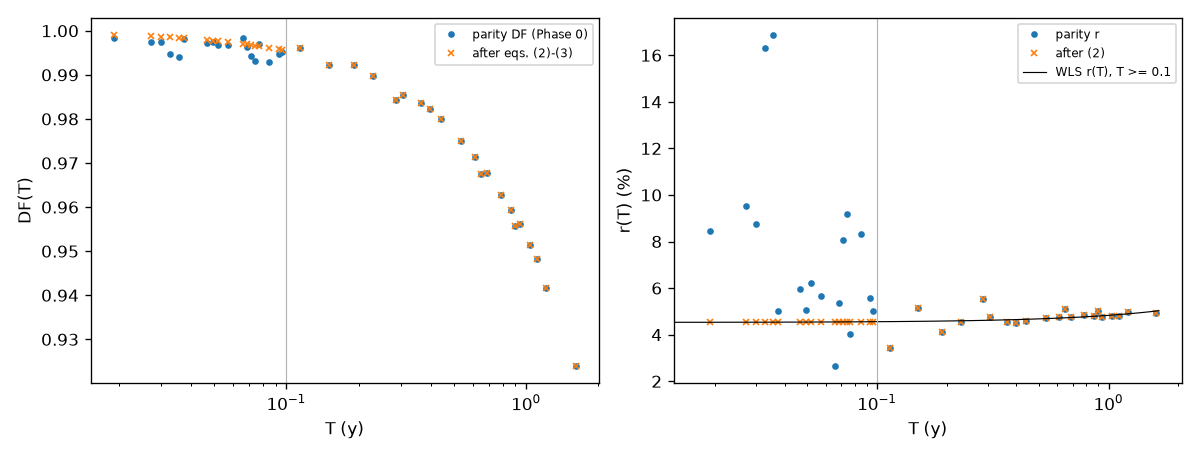
\includegraphics[width=\textwidth]{calibration_df_r_20261106_2213.png}
\caption{Term structure of the discount factors (left) and of the zero rates (right), on a logarithmic scale in $T$.
Dots: parity values; crosses: after the short-end correction; line: the WLS curve fitted for $T\ge0.1$ (vertical
line). Below $0.1$ years the parity rates swing between 2.6\% and 16.9\%; after the correction they lie on the
curve.}
\label{fig:df-r}
\end{figure}

\begin{idea}
The correction changes almost nothing in the calibration numbers (the call/put gap barely decreases), but it removes
meaningless rates and a systematic error on the whole smile of the weekly expiries. It is the kind of correction that
is made \emph{before} inverting the prices, because afterwards the error would be hidden inside the model
parameters.
\end{idea}

\section{The OTM surface}
\label{sec:superficie-otm}
For the calibration only \textbf{out-of-the-money} options are kept: puts for $K<F$, calls for $K\ge F$
(\code{data.select\_otm}).

\begin{perche}
The price of an ITM option is almost all intrinsic value. The bid/ask spread, which is in absolute terms, falls
entirely on the small time value and becomes a large error on the implied volatility (Chapter~\ref{cap:black}). OTM
options are more liquid and have tighter relative spreads.

And no information is lost: if $F$ and $\DF$ are consistent with parity, the call and the put at the same strike have
the same implied volatility.
\end{perche}

\section{The static-arbitrage filter}
\label{sec:filtro-arbitraggio}
Even after cleaning, some stale quotes remain that create obvious arbitrages. The parity rejection rule only sees the
20-pair window; the wings of the surface and the strikes without a twin leg escape it.

For two strikes $K_i<K_j$ of the same expiry and of call type, using \emph{tradable} prices (bid and ask, not the
mid):
\begin{itemize}
\item \emph{monotonicity:} if $\text{bid}_j>\text{ask}_i$, I buy the low-strike call and sell the high-strike one,
collecting a credit, with a future payoff $\ge0$: an arbitrage;
\item \emph{vertical spread:} if $\text{bid}_i-\text{ask}_j>K_j-K_i$, I sell a spread for more than its maximum
payoff.
\end{itemize}
For puts the conditions are mirrored: $\text{bid}_i>\text{ask}_j$ or $\text{bid}_j-\text{ask}_i>K_j-K_i$. Using
$\DF\le1$ makes the conditions independent of any model.

All pairs of strikes are checked, not only adjacent ones, because a stale quote can violate monotonicity with a
distant strike.

The function \code{data.remove\_static\_arbitrage} ``greedily'' removes the quote involved in the largest number of
violations (ties broken by the least recently traded, then by the lowest strike) and repeats until none are left. A
stale quote conflicts with every good quote it crosses, so it has far more violations than the others.

\begin{esempio}
On the \mbox{2027-03-31} expiry the 7615 call had a bid of 434.4 while the 7610 call was offered at 258.5: buying the
7610 and selling the 7615 would have yielded a credit of 175.9 points with a payoff that is never negative. Its
implied volatility was 26.7\%, against about 17\% for its neighbors.

In total 25 quotes were removed on 5 expiries. They were all stale (last trade between July and September 2026) and
14.4--179.9 points away from the level indicated by their neighbors. An independent check, with a different
algorithm, confirmed that the resulting surface has no violations and that each of the 25 removals is necessary:
putting any one of them back makes the arbitrage reappear.
\end{esempio}

\begin{attenzione}
The filter guarantees only monotonicity and vertical spreads. Convexity (butterfly) and calendar arbitrage are
checked, as diagnostics, in the calibration (Chapter~\ref{cap:calibrazione}). On the final surface there are no
violations executable at bid/ask, neither calendar (11{,}054 points) nor butterfly (7547 triples). On the mids,
however, 2126 triples violate convexity, all by less than half the spread of the butterfly (at most 0.427 times): the
mid is not a tradable price. Saying ``the surface is arbitrage-free'' without these qualifications would be wrong.
\end{attenzione}

\begin{riassunto}
\begin{itemize}
\item One family per date (AM/PM), ACT/365F time to the settlement instant (watch out for early closes).
\item $C-P=\DF F-\DF K$: a straight line in $K$; slope $=-\DF$, zero $=F$. $F$ is robust (because $\bar y\approx0$),
short-dated $\DF$ is not.
\item Robust regression (Theil--Sen, MAD) and rejection only outside the bid/ask band; the acceptance rules have an
economic content and do not stop at $R^2$. 39 expiries out of 40 remain.
\item At the short end the $\DF$s are replaced by a curve $\hat r(T)=4.527\%+0.304\%\,T$ fitted on $T\ge0.1$, and the
forwards are recomputed at fixed $\DF$: shifts below one index point, pairs always inside their bands.
\item OTM surface, static-arbitrage filter on bid/ask: 7625 quotes on 39 expiries.
\end{itemize}
\end{riassunto}

\begin{domande}
\begin{enumerate}
\item How do you obtain $F$ and $\DF$ from an option chain without knowing $r$ and $q$?
\item Why is the forward identified even at very short expiries while the discount factor is not? \emph{Hint:}
\eqref{eq:se-F} with $\bar y\approx0$.
\item Is the 16.9\% rate on a two-week expiry real? \emph{Hint:} no, the slope signal is below the resolution of the
quotes; the long rate is the box-spread rate.
\item Why does the rejection rule require the line to be outside the bid/ask band?
\item Derive the shift \eqref{eq:spostamento-F} of the forward when $\DF$ is changed. Why is it small?
\item How much does a 0.4\% error on $\DF$ move the ATM volatility? And an error on $F$? \emph{Hint:}
\eqref{eq:dsigma-dDF} and \eqref{eq:dsigma-dF}.
\item Why are bid and ask, and not the mid, used in the arbitrage filter? \emph{Hint:} only an arbitrage executable at
the quoted prices is a true arbitrage.
\end{enumerate}
\end{domande}

\chapter{The Black model (Black--Scholes on the forward)}
\label{cap:black}

The Black-76 model is the ``building block'' on which the whole project rests: every other model is compared with
it, implied volatilities are defined through it, and almost every exotic product uses it as an oracle in some limit.
In this chapter we derive the pricing formula, the Greeks, Black's equation, the gamma--theta link and the algorithm
that inverts the formula (implied volatility).

\section{Assumptions}
Under the $T$-forward measure the forward follows a driftless geometric Brownian motion, as in \eqref{eq:gbm}:
$\mathrm{d}F_t=\sigma F_t\dd W_t$, with $F_T=S_T$. The price of a European option is
\[
V_0=\DF\cdot\E^T\big[(\theta(F_T-K))^+\big].
\]
Inputs: $F,K>0$, $T>0$, $\DF$, $\sigma>0$. No $r$, no $q$.

Notation: $x=\ln(F/K)$ (the call is ITM if $x>0$), $s=\sigma\sqrt T$ (total volatility),
\begin{equation}
d_{1,2}=\frac{\ln(F/K)}{\sigma\sqrt T}\pm\frac{\sigma\sqrt T}{2}=\frac{x}{s}\pm\frac{s}{2},\qquad d_1-d_2=s.
\end{equation}

\section{The pricing formula, step by step}
\begin{proposizione}[Black-76 formula]
\begin{equation}\label{eq:black}
\boxed{V=\DF\,\theta\,\big[F\,\Phi(\theta d_1)-K\,\Phi(\theta d_2)\big]}
\end{equation}
\end{proposizione}

\begin{proof}[Derivation for the call ($\theta=+1$)]
\textbf{Step 1: split the payoff.} Write
\[
(F_T-K)^+=F_T\,\ind\{F_T>K\}-K\,\ind\{F_T>K\},
\]
so that
\[
\E^T[(F_T-K)^+]=\underbrace{\E^T[F_T\ind\{F_T>K\}]}_{(I)}-K\,\underbrace{\Q^T(F_T>K)}_{(II)} .
\]
\textbf{Step 2: the term (II).} From \eqref{eq:gbm-sol}, $F_T=F e^{sZ-s^2/2}$. Then
\[
F_T>K\iff sZ-\tfrac{s^2}{2}>\ln\tfrac KF\iff Z>\frac{-x+s^2/2}{s}=-d_2 .
\]
Hence $\Q^T(F_T>K)=\Q(Z>-d_2)=\Phi(d_2)$.

\textbf{Step 3: the term (I) via a change of measure.} Write $F_T=F\cdot e^{sZ-s^2/2}$ and apply \eqref{eq:tilt}
with $f(Z)=\ind\{Z>-d_2\}$:
\begin{align*}
\E\big[Fe^{sZ-s^2/2}\ind\{Z>-d_2\}\big]&=F\,\E\big[\ind\{Z+s>-d_2\}\big]\\
&=F\,\Q(Z>-d_2-s)=F\,\Phi(d_2+s)=F\,\Phi(d_1).
\end{align*}
\textbf{Step 4.} Multiply by $\DF$: $C=\DF[F\Phi(d_1)-K\Phi(d_2)]$. For the put, repeat the computation on the event
$\{F_T<K\}$, or use parity; this gives \eqref{eq:black} with $\theta=-1$.
\end{proof}

\begin{idea}[title={What $\Phi(d_1)$ and $\Phi(d_2)$ are}]
\begin{itemize}
\item $\Phi(d_2)=\Q^T(F_T>K)$ is the probability of exercise \emph{under the forward measure}, not a real-world
forecast. $\DF\,\Phi(d_2)=-\partial C/\partial K$ is the price of a \emph{digital} option (it pays 1 if $F_T>K$).
\item $\Phi(d_1)$ is the probability of the same event under the ``share measure'' (numéraire = underlying).
$\DF\,\Phi(d_1)$ is the delta with respect to the forward.
\end{itemize}
\end{idea}

\subsection{Normalized form and symmetries}
Dividing by $\DF\sqrt{FK}$ and using $\sqrt{F/K}=e^{x/2}$:
\begin{equation}\label{eq:black-norm}
V=\DF\sqrt{FK}\;b_\theta(x,s),\qquad b_\theta(x,s)=\theta\big[e^{x/2}\Phi(\theta d_1)-e^{-x/2}\Phi(\theta d_2)\big],
\end{equation}
with the symmetry $b_{-1}(x,s)=b_{+1}(-x,s)$.
The price therefore depends on only \emph{two} numbers: the moneyness $x$ and the total volatility $s$. Other
identities that are useful as tests: homogeneity $V(\lambda F,\lambda K)=\lambda V$; swap $C(F,K)=P(K,F)$; put--call symmetry
$C(F,K)=(K/F)\,P(F,F^2/K)$.

\subsection{Limits}
For $0<\sigma<\infty$: $(F-K)^+<c<F$ and $(K-F)^+<p<K$ (undiscounted prices). As $\sigma\to0$ the price tends to
$\DF$ times the intrinsic value; as $\sigma\to\infty$ the call tends to $\DF\,F$ and the put to $\DF\,K$. At the money
($x=0$) the price is exactly $C=\DF\,F\,\mathrm{erf}\big(s/(2\sqrt2)\big)$; to first order
\begin{equation}\label{eq:brenner}
C_{\text{ATM}}\approx\DF\,F\,\frac{s}{\sqrt{2\pi}}\approx0.4\,\DF\,F\,\sigma\sqrt T\qquad\text{(Brenner--Subrahmanyam)}.
\end{equation}

\section{The Greeks}
The \textbf{Greeks} are the derivatives of the price with respect to the inputs: they measure risk and tell us how
to hedge it. In the project they are derivatives with respect to the forward $F$ (with $K,T,\DF,\sigma$ fixed).

\subsection{An identity that simplifies everything}
\begin{equation}\label{eq:identita-phi}
F\,\varphi(d_1)=K\,\varphi(d_2).
\end{equation}
\emph{Proof.} Since $d_1-d_2=s$ and $d_1+d_2=2x/s$,
\[
\frac{\varphi(d_2)}{\varphi(d_1)}=e^{(d_1^2-d_2^2)/2}=e^{(d_1-d_2)(d_1+d_2)/2}=e^{s\cdot(2x/s)/2}=e^{x}=\frac FK .
\]

\emph{Consequence.} When \eqref{eq:black} is differentiated with respect to an input $y$, the terms arising from
$\partial_yd_1$ and $\partial_yd_2$ combine into $\DF\,F\varphi(d_1)\,\partial_y(d_1-d_2)=\DF\,F\varphi(d_1)\,\partial_ys$.
So \emph{only the change in $s$ matters}. If $y=F$, $s$ does not change and those terms vanish.

\subsection{The formulas}
\begin{align}
\Delta_F&=\frac{\partial V}{\partial F}=\theta\,\DF\,\Phi(\theta d_1),\label{eq:delta}\\
\Gamma_F&=\frac{\partial^2V}{\partial F^2}=\frac{\DF\,\varphi(d_1)}{F\,\sigma\sqrt T}\quad\text{(same for call and put)},\label{eq:gamma}\\
\vega&=\frac{\partial V}{\partial\sigma}=\DF\,F\,\varphi(d_1)\sqrt T\quad\text{(same for call and put)},\label{eq:vega}\\
\Theta&=\Theta_0+rV,\qquad\Theta_0=-\frac{\DF\,F\,\varphi(d_1)\,\sigma}{2\sqrt T},\qquad r=-\frac{\ln\DF}{T}.\label{eq:theta}
\end{align}
Derivations: for the delta, $y=F$ and the $\partial d$ terms vanish; for the gamma, $\partial_F\Phi(d_1)=\varphi(d_1)/(Fs)$;
for the vega, $\partial_\sigma s=\sqrt T$; for $\Theta_0$, $\partial_Ts=\sigma/(2\sqrt T)$ at fixed $\DF$. The vega is
``per unit of volatility'': per ``vol point'' divide by 100 (on Hull's Greeks example in the next section the vega is
12.1055, that is, 0.121 per vol point).

Check identities: $\vega=\sigma T F^2\Gamma_F$ (long gamma $\Leftrightarrow$ long vega for a single option);
$\Delta_C-\Delta_P=\DF$; $\partial C/\partial K=-\DF\,\Phi(d_2)$; $\partial^2C/\partial K^2=\DF\,\varphi(d_2)/(Ks)$ (the
lognormal density, consistent with Breeden--Litzenberger).

\subsection{Theta and its convention}
The project's theta is $\Theta=\partial V/\partial t$ in calendar time, per year (divide by 365 for a daily theta).
It holds fixed $F$ (the forward for the same expiry date), $K$, $\sigma$ and the zero rate $r=-\ln\DF/T$. So, as time
passes, the discount factor $\DF=e^{-r(T-t)}$ ``grows'' towards 1 and contributes $+rV$: this is the return on the
premium paid. The part at fixed $\DF$, $\Theta_0$, is pure time decay.

\begin{perche}[title={Why this convention?}]
It is exactly the $\mathrm{d}t$ term of Black's equation (next section): under $\Q^T$ the forward has no drift, so
this is the theta that enters the expected P\&L of a hedged option. The $rV$ term is offset by the cost of funding
the premium, and $\Theta_0$ remains.
\end{perche}

\begin{attenzione}[title={The project's theta is not Hull's}]
For a deep ITM call the theta can be \emph{positive}: $rV$ exceeds $|\Theta_0|$. In the project this happens at
50.6\% of the ITM points of the test grid. Only $\Theta_0$ is always negative; on the OTM options of the grid the
ratio $rV/|\Theta_0|$ reaches at most 0.688, so there $\Theta<0$ always.

Hull, by contrast, holds spot, $r$ and $q$ fixed. The link is derived step by step. With a continuous-yield model
$F=S\,e^{(r-q)(T-t)}$; at fixed $S$ the forward moves in time with $\partial F/\partial t=-(r-q)F$. By the chain
rule
\begin{equation}\label{eq:theta-spot}
\Theta_S=\Theta+\Delta_F\,\frac{\partial F}{\partial t}=\Theta-(r-q)\,F\,\Delta_F .
\end{equation}
Likewise $\Delta_S=\Delta_F\,\partial F/\partial S=e^{-qT}\Phi(d_1)$ for the call. On Hull's Greeks example
($S=49$, $K=50$, $r=5\%$, $q=0$, $\sigma=20\%$, $T=20/52$) the kernel theta is $-3.027$/year;
\eqref{eq:theta-spot} gives $-4.30533$/year, that is, $-0.0117954$ per day, which is Hull's value ($-4.31$/year).
\end{attenzione}

\section{Black's equation and the gamma--theta link}
By Feynman--Kac \eqref{eq:feynman-kac}, the undiscounted price $v=V/\DF$ satisfies
$\partial_tv+\frac12\sigma^2F^2v_{FF}=0$. Multiplying by $\DF$ (and recalling that $\partial_t\DF=r\DF$):
\begin{equation}\label{eq:pde-black}
\Theta+\tfrac12\sigma^2F^2\Gamma_F-rV=0 .
\end{equation}
\subsection{The P\&L of a delta-hedged option}
I buy an option and sell $\Delta_F$ forwards (or futures) to neutralize the risk to first order. Over an interval
$\Delta t$, by a Taylor expansion:
\[
\mathrm{d}\Pi\approx\underbrace{\Delta_F\,\Delta F-\Delta_F\,\Delta F}_{=0\ \text{(hedge)}}+\tfrac12\Gamma_F(\Delta F)^2+\Theta_0\,\Delta t .
\]
Using \eqref{eq:pde-black} ($\Theta_0=-\frac12\sigma^2F^2\Gamma_F$, once the cost of funding the premium $rV$ is
removed):
\begin{equation}\label{eq:pnl-gamma}
\boxed{\mathrm{d}\Pi=\tfrac12\Gamma_F F^2\Big[\Big(\frac{\Delta F}{F}\Big)^2-\sigma^2\Delta t\Big]}
\end{equation}
\begin{idea}[title={Key idea: ``gamma pays for theta''}]
Whoever is long a hedged option makes money if the \emph{realized} variance $(\Delta F/F)^2$ exceeds the
\emph{implied} one $\sigma^2\Delta t$, and loses otherwise. Theta is the ``rent'' paid for owning gamma. The gain is
weighted by gamma, so it is path-dependent: a large move far from the strike (where gamma is small) earns little.
For short-dated ATM options gamma and theta grow like $1/\sqrt T$ while vega decreases like $\sqrt T$: a portfolio
long the 1-year option and short the 1-month option is short gamma and long vega.
\end{idea}

\section{Implied volatility}
\subsection{The problem}
Given a market price $V^m$, find $\sigma$ such that $V_{\text{Black}}(\sigma)=V^m$. The problem is solved in
normalized form. The steps:
\begin{enumerate}
\item Undiscounted price $v=V/\DF$; if $v$ does not lie strictly between the intrinsic value $\iota$ and $F$ (call)
or $K$ (put), no volatility exists: \code{NaN} is returned with a status code.
\item Always switch to the \textbf{OTM} option (thanks to parity): $\beta=(v-\iota)/\sqrt{FK}$.
\item Solve $b(s):=b_{+1}(-|x|,s)=\beta$ for the unknown $s$, and finally $\sigma=s/\sqrt T$.
\end{enumerate}

\subsection{Existence and uniqueness}
Differentiating the normalized form and using \eqref{eq:identita-phi}:
\begin{equation}\label{eq:vega-norm}
b'(s)=\frac{1}{\sqrt{2\pi}}\exp\!\Big(-\frac{x^2}{2s^2}-\frac{s^2}{8}\Big)>0,\qquad
b''(s)=b'(s)\Big(\frac{x^2}{s^3}-\frac s4\Big).
\end{equation}
$b$ is strictly increasing, starts from $0$ (as $s\to0$, the OTM option is worth zero) and tends to $e^{-|x|/2}$:
every admissible $\beta$ has \emph{exactly one} solution. The true vega is $\vega=\DF\sqrt{FK}\sqrt T\,b'(s)$.

\subsection{Newton without surprises (Manaster--Koehler)}
Newton's method $s_{n+1}=s_n-(b(s_n)-\beta)/b'(s_n)$ converges quickly but can diverge from a bad start. From
\eqref{eq:vega-norm}: $b''=0$ at $s_c=\sqrt{2|x|}$; $b$ is \textbf{convex} on $(0,s_c)$ and \textbf{concave} on
$(s_c,\infty)$, and vega is maximal at $s_c$.
\begin{perche}[title={Why start from the inflection point}]
\begin{itemize}
\item If the root lies in the concave part ($\beta>b(s_c)$), the tangents lie \emph{above} the graph: every Newton
step lands \emph{before} the root, and the iterates increase monotonically towards it.
\item If the root lies in the convex part ($\beta<b(s_c)$), the tangents lie \emph{below}: the iterates decrease
monotonically towards the root.
\end{itemize}
In both cases the root is never ``overshot''. At the money ($x=0$) $s_c=0$, and the exact inverse
$s=2\sqrt2\,\mathrm{erfinv}(\beta)$ is used instead.
\end{perche}
The project's solver adds a \emph{safeguard} anyway: it keeps a bracket $[\ell,h]$ containing the root (initially
$[0,10\sqrt T]$) and, if Newton leaves the bracket, it takes a bisection step. Elements that have not converged after
100 iterations go to Brent's method (which was never needed on the test grid).

\subsection{Why always invert the OTM option}
By parity, the undiscounted OTM price equals the time value of the ITM option at the same strike, and the vega is the
same. But an ITM price carries an absolute rounding error $\approx\varepsilon\max(F,K)$, which ends up \emph{entirely}
on the time value. The error on the volatility is
\begin{equation}\label{eq:errore-iv}
|\delta\sigma|\approx\frac{|\delta v_{\text{time value}}|}{\sqrt{FK}\sqrt T\,b'(s)} .
\end{equation}
For an OTM input $\delta v\approx\varepsilon v$, for an ITM input $\delta v\approx\varepsilon\max(F,K)$: the a priori
estimate is $\lesssim10^{-14}$ against $\sim10^{-12}$.

Measured in the project, on the test grid ($147{,}600$ points per option type): round-trip error at most
${1.07\times10^{-14}}$ for OTM inputs and ${8.23\times10^{-13}}$ for ITM inputs, against a threshold of $10^{-10}$.
An independent check on $300{,}000$ random off-grid points gave ${1.05\times10^{-14}}$ and ${6.54\times10^{-13}}$. The
measurements confirm the error model.

In the extreme wings the vega vanishes: tiny errors on the price become huge errors on the volatility, and below
machine precision there is no information left.

\section{Checking the Greeks with finite differences}
The Greek formulas are checked by comparing them with numerical derivatives:
\begin{equation}\label{eq:diff-finite}
D_1f=\frac{f(u+h)-f(u-h)}{2h},\qquad D_2f=\frac{f(u+h)-2f(u)+f(u-h)}{h^2}.
\end{equation}

\begin{perche}[title={How to choose the step $h$}]
Two errors compete.
\begin{itemize}
\item The truncation (Taylor) error is $\approx h^2|f'''|/6$ for $D_1$ and $\approx h^2|f''''|/12$ for $D_2$: it grows
with $h$.
\item The rounding error is $\approx\varepsilon|f|/h$ for $D_1$ and $\approx4\varepsilon|f|/h^2$ for $D_2$: it grows
as $h$ decreases.
\end{itemize}
Minimizing the sum gives $h\propto\varepsilon^{1/3}$ for $D_1$ and $h\propto\varepsilon^{1/4}$ for $D_2$. An $h$ that
is too small is worse than one that is too large. The steps are expressed in the natural scale of the variable: for
$F$ a multiple of $F\sigma\sqrt T$ is used, which is one standard deviation of the forward.
\end{perche}

\paragraph{Theta by finite differences.} For the theta, $T$ and $\DF$ must be moved together at fixed $r$:
\begin{equation}\label{eq:theta-fd}
\Theta_{\text{FD}}=\frac{V(F,K,T-h,\DF\,e^{+rh},\sigma)-V(F,K,T+h,\DF\,e^{-rh},\sigma)}{2h}.
\end{equation}
Moving only $T$ measures $\Theta_0$ and is off by $rV$.

\begin{progetto}[title={In the qpricer project: the gamma that ``would not pass''}]
\textbf{The symptom.} With the step originally planned, $h=10^{-4}F\sigma\sqrt T$, the finite-difference gamma was off
by up to ${1.773\times10^{-5}}$ in relative terms (threshold $10^{-5}$), at 78 points out of $147{,}600$, all with
$\sigma\sqrt T\approx0.007$.

\textbf{The diagnosis.} The analytic gamma was right: the identity $\vega=\sigma TF^2\Gamma$ held below $10^{-12}$,
and larger steps converged to it. It was \emph{the reference that was noisy}. At the worst point the price noise was
about $600\,\varepsilon V$, not $\varepsilon V$, because of the cancellation in $F\Phi(d_1)-K\Phi(d_2)$. The rounding
term $4\varepsilon|f|/h^2$ was therefore 600 times larger than expected, and the optimal step grows by
$600^{1/4}\approx5$.

\textbf{The new step, step by step.} Write $h=c\,F\sigma\sqrt T$ and model the worst error on the grid as
$A c^2+B/c^2$ (truncation plus rounding).
\begin{enumerate}
\item $A=4.47$ is measured at the corner where truncation dominates ($\sigma=1$, $T=5$, $z=3$, with
$c={2\times10^{-3}}$).
\item $B={1.77\times10^{-13}}$ is measured at the corner where rounding dominates (with $c=10^{-4}$).
\item The minimum of $Ac^2+B/c^2$ is at $c^*=(B/A)^{1/4}={4.46\times10^{-4}}$, where it equals
$2\sqrt{AB}\approx{1.8\times10^{-6}}$.
\end{enumerate}
With $c={4.5\times10^{-4}}$ the measured error is ${9.96\times10^{-7}}$. The threshold was not loosened and the grid
was not changed: the reference changed, not the criterion. An independent check confirmed the analytic gamma to
${8.9\times10^{-15}}$ against finite differences computed with 60 decimal digits, and also checked the gamma of the
ITM options (${1.24\times10^{-6}}$ with its own Richardson scheme).
\end{progetto}

\section{Main numerical pitfalls}
\begin{enumerate}
\item \textbf{Normal tails.} Never $1-\Phi(d)$; use the form with $\theta$, \code{ndtr(theta*d)}.
\item \textbf{ITM cancellation.} The time value of an ITM option, the finite-difference gamma of an ITM option and
the implied volatility from an ITM price all have an absolute error $\approx\varepsilon(F+K)$. One works on the OTM
side. A measured example: for an ITM quote with $3<|z|<7.5$, where $z=\ln(K/F)/(\sigma\sqrt T)$, the solver returns a
volatility with status ``converged'' but with an error that can reach ${2.0\times10^{-4}}$ in absolute terms
($\sigma=1$, $T=5$, $z=6.5$). This is not a defect of the solver: the error matches the conditioning limit
$\varepsilon\max(v,F,K)/(\vega/\DF)$ of \eqref{eq:errore-iv}. It is, however, an unflagged error, a known and
unresolved limitation; the calibration is not affected, because it uses only OTM quotes (Chapter~\ref{cap:dati}).
\item \textbf{Parity to $10^{-12}$.} Computing call and put separately, the error is
$\approx c\,\varepsilon\,\DF(F+K)$ with $c\approx2$--4. For strikes very large relative to $F=100$ (up to
$K\approx{8.2\times10^4}$ in the test domain) the ulp of $K$ already exceeds $10^{-12}$, and that threshold is not
representable in double precision. This is why parity is checked to $10^{-12}$ for $K/F\in[0.25,4]$, and elsewhere
at the limit of double precision, $4$ ulp of $\DF\max(F,K)$. Computing the put as $C-\DF(F-K)$ would turn the test
into a tautology.
\item \textbf{$s\to0$.} $d_{1,2}=0/0$ when $F=K$. The code substitutes the limits ($+\infty$ for $x>0$, $-\infty$
for $x<0$, $0$ for $x=0$), and the formulas automatically return the correct limits, with no special branches. At the
money the vega at $\sigma=0$ is the right derivative $\DF\,F\sqrt T/\sqrt{2\pi}$, consistent with
\eqref{eq:brenner}.
\item \textbf{Deep wings.} \code{ndtr} returns 0 below $d\approx-37.5$, even though $\Phi$ would still be
representable down to $d\approx-38.5$. If $\Phi(d_2)$ underflows and $\Phi(d_1)$ does not, the normalized function
$b(s)$ loses its second term and comes out up to about 17 times too large: the solver converges on a wrong function.
An independent check showed that, for OTM prices below about $10^{-280}$, this produced a wrong volatility, even
$\sigma=0$, without flagging it. The fix: the root is accepted only if $s>0$ and
$\Phi(d_2)\ge10^3\cdot\text{(smallest normal number)}\approx{2.2\times10^{-305}}$; otherwise the result is \code{NaN}
with a dedicated status and a warning. No quoted price lies in that region, but the rule ``never a wrong number
silently'' applies everywhere.
\item \textbf{Impossible prices.} If the price does not lie strictly between the intrinsic value and $F$ (call) or
$K$ (put), or the volatility exceeds the cap $\sigma_{\max}=10$, the solver returns \code{NaN} with a status code and a
warning. The status is per element: a single stale or crossed quote does not stop the inversion of an entire chain,
and it is never silently ``adjusted''. Invalid market inputs ($F\le0$, $T\le0$, \dots), by contrast, raise an error:
they are programming errors, not data.
\end{enumerate}

\begin{progetto}[title={In the qpricer project: Phase 1 results}]
The numbers come from \code{scripts/phase1\_gates.py} and from an independent check, which uses a Black formula
computed with 60 decimal digits, the complex-step method and its own bisection solver.
\begin{center}
\small
\begin{tabularx}{\textwidth}{X l l}
\toprule
check & measured & threshold\\
\midrule
parity, $K/F\in[0.25,4]$, ${2\times10^5}$ points & ${1.137\times10^{-13}}$ & $10^{-12}$\\
parity, whole test domain & 2.25 ulp (${1.455\times10^{-11}}$) & 4 ulp\\
implied volatility, round trip, OTM input & ${1.07\times10^{-14}}$ & $10^{-10}$\\
implied volatility, round trip, ITM input & ${8.23\times10^{-13}}$ & $10^{-10}$\\
delta vs finite differences (relative) & ${2.05\times10^{-8}}$ & $10^{-5}$\\
gamma vs finite differences (relative) & ${9.96\times10^{-7}}$ & $10^{-5}$\\
vega vs finite differences (relative) & ${2.96\times10^{-7}}$ & $10^{-5}$\\
theta vs finite differences (relative) & ${1.69\times10^{-8}}$ & $10^{-5}$\\
Greeks vs 60-digit reference & $\le{5.1\times10^{-14}}$ & ---\\
Hull's example (Black-76, $F=K=20$) & $1.1166414\ldots$ vs $1.1166$ & $\pm{0.5\times10^{-4}}$\\
\bottomrule
\end{tabularx}
\end{center}
On $2\times147{,}600$ elements the Newton solver uses at most 12 evaluations (6.95 on average), and the Brent fallback
is never called. The file \code{tests/golden/bsm\_black76.json} freezes 12 cases (price and Greeks) computed in
extended precision; the implementation reproduces them to within $10^{-11}$ relative.
\end{progetto}

\begin{riassunto}
\begin{itemize}
\item $V=\DF\,\theta\,[F\,\Phi(\theta d_1)-K\,\Phi(\theta d_2)]$; it depends only on $x=\ln(F/K)$ and $s=\sigma\sqrt T$.
\item $F\,\varphi(d_1)=K\,\varphi(d_2)$ simplifies all the Greeks. $\vega=\sigma TF^2\Gamma$.
\item Theta at fixed $F$ and $r$: $\Theta=\Theta_0+rV$, which can be positive for ITM options; Hull's differs by
$(r-q)F\Delta_F$.
\item Black's PDE $\Rightarrow$ hedged P\&L $=\frac12\Gamma F^2[(\Delta F/F)^2-\sigma^2\Delta t]$.
\item Implied volatility is unique; Newton started from the point of maximum vega converges monotonically; invert the
OTM option.
\item Finite differences: the step balances truncation and rounding, and must be chosen on the true price noise.
\end{itemize}
\end{riassunto}

\begin{domande}
\begin{enumerate}
\item Derive Black's formula for the call using the change of measure. Where does $\Phi(d_1)$ come in?
\item You are long an ATM call, delta-hedged every day. What is your P\&L? \emph{Hint:} \eqref{eq:pnl-gamma}.
\item Why does Newton start from $s_c=\sqrt{2|x|}$ for the implied volatility?
\item The theta of an ITM call is positive: is that a mistake? \emph{Hint:} no, $\Theta=\Theta_0+rV$ and $rV$ can
exceed $|\Theta_0|$.
\item How does one go from the kernel theta to Hull's? \emph{Hint:} \eqref{eq:theta-spot}.
\item The finite-difference gamma fails the test: should the threshold be loosened? \emph{Hint:} no; analyze the
noise of the reference and choose the optimal step.
\end{enumerate}
\end{domande}


\part{Stochastic volatility and Monte Carlo}
\chapter{The volatility smile and the Heston model}
\label{cap:heston}

This chapter presents the Heston (1993) model: the phenomenon it must capture (the \emph{skew}), the closed-form
characteristic function, and two independent Fourier engines, COS and Lewis. Monte Carlo is covered in
Chapter~\ref{cap:mc}.

\section{Why Black is not enough: smile and skew}
If the Black model were correct, inverting the market prices of all options of one expiry would always return the
same volatility. On the SPX index, this is what happens instead:
\begin{itemize}
\item implied volatility is \textbf{decreasing in $K$} (\emph{skew}): OTM puts are more expensive than OTM calls;
\item the skew is \textbf{steeper at short expiries} and flattens as $T$ grows;
\item the ATM level also varies with expiry (\emph{term structure}).
\end{itemize}
The function $(K,T)\mapsto\sigma_{\text{impl}}(K,T)$ is called the \textbf{implied-volatility surface}.

\begin{perche}[title={Why is there a skew?}]
Recalling Breeden--Litzenberger \eqref{eq:breeden}, a negative skew means that the market density has a
\textbf{heavier left tail} than the lognormal: crashes are more likely than Black says.

The economic mechanism is the \emph{leverage effect}: when the index falls, volatility rises. We therefore need a
random volatility that is \emph{negatively correlated} with the price.
\end{perche}

\section{The Heston model}
Heston makes the instantaneous variance random and correlates it with the price. It is the simplest model that
produces the skew and still admits prices in almost closed form: the variance reverts to a long-run level, the
negative correlation generates the leverage effect, and the \emph{affine} structure of the equations makes the
characteristic function of the log-price known in closed form. With only five parameters the model describes the
whole surface, that is, all expiries at once.

\subsection{The dynamics}
We work under the $T$-forward measure $\Q^T$, as in Chapter~\ref{cap:black}. With deterministic rates and carry, the
risk-neutral Heston dynamics carry over unchanged to the forward $F_t=F(t,T)$:
\begin{equation}\label{eq:heston}
\begin{aligned}
\mathrm{d}F_t&=\sqrt{v_t}\,F_t\dd W^F_t,\\
\mathrm{d}v_t&=\kappa(\theta-v_t)\dd t+\xi\sqrt{v_t}\dd W^v_t,\qquad \dd\langle W^F,W^v\rangle_t=\rho\dd t .
\end{aligned}
\end{equation}
The instantaneous \emph{variance} $v_t$ follows a Cox--Ingersoll--Ross (CIR) process, that is, a mean-reverting
diffusion with volatility proportional to $\sqrt{v_t}$. The five parameters are summarized in
Table~\ref{tab:heston-parametri}.

\begin{table}[htbp]
\centering
\small
\caption{The parameters of the Heston model and their effect on the smile.}
\label{tab:heston-parametri}
\begin{tabularx}{\textwidth}{@{}>{$}c<{$}l>{\raggedright\arraybackslash}X@{}}
\toprule
\text{par.} & name & effect on the smile \\
\midrule
v_0 & initial variance & ATM level of short expiries \\
\theta & long-run variance & ATM level of long expiries \\
\kappa & mean-reversion speed & how fast $v$ moves from $v_0$ to $\theta$; how fast the skew flattens with $T$ \\
\xi & volatility of variance (\emph{vol-of-vol}) & fatter tails on both sides: curvature of the smile \\
\rho & price--variance correlation & slope: $\rho<0$ creates the negative skew \\
\bottomrule
\end{tabularx}
\end{table}

The required domain is $\kappa-\rho\xi>0$, automatic for $\rho\le0$ (the SPX case). The code rejects other inputs:
for $\kappa-\rho\xi\le0$ some expressions in the characteristic function become $0/0$.

\subsection{Expected variance and integrated variance}
Taking the expectation of the $v$ equation (the $\mathrm{d}W$ term has zero mean) gives an ordinary differential
equation, $\frac{\mathrm{d}}{\mathrm{d}t}\E v_t=\kappa(\theta-\E v_t)$, with solution
\begin{equation}\label{eq:var-attesa}
\bar v(t):=\E v_t=\theta+(v_0-\theta)e^{-\kappa t}.
\end{equation}
Integrating over $[0,T]$ and setting $\tau_\kappa=(1-e^{-\kappa T})/\kappa$:
\begin{equation}\label{eq:sigma-bar}
\bar\Sigma:=\int_0^T\bar v(t)\dd t=\theta T+(v_0-\theta)\,\tau_\kappa .
\end{equation}
$\bar\Sigma$ is the ``expected total variance''. The effective volatility $\sigma_{\text{eff}}=\sqrt{\bar\Sigma/T}$
will come back in the limit $\xi\to0$.

\subsection{The Feller condition}
The Feller ratio $\nu_F=2\kappa\theta/\xi^2$ decides whether the variance can reach zero.
\begin{itemize}
\item If $\nu_F\ge1$, the drift $\kappa\theta$ near 0 is strong enough to prevent it.
\item If $\nu_F<1$, the variance hits 0 and immediately leaves it (the boundary is instantaneously reflecting).
\end{itemize}
\begin{attenzione}
Realistic SPX calibrations typically \emph{violate} Feller: enough curvature requires a large $\xi$. This does
\textbf{not} cause problems for the Fourier methods of this chapter, because the characteristic function is the same
whether or not zero is attainable. It does, however, cause problems for Monte Carlo (Chapter~\ref{cap:mc}).

Imposing Feller in calibration would spoil the fit of the short-dated skew: in the project the ratio $\nu_F$ is
\emph{reported}, not imposed.
\end{attenzione}

\section{The Heston characteristic function}
In Heston the density of $F_T$ is not known in closed form, but the characteristic function is, because the model is
\textbf{affine}: the drift and the instantaneous variance are linear functions of the state $(x,v)$.

\subsection{Step-by-step derivation}
Let $X=\ln(F_T/F)$ be the log-return of the forward and $\varphi(u)=\E^T[e^{iuX}]$ its characteristic function (CF).
In the state $x_t=\ln(F_t/F)$, by Itô, $\mathrm{d}x=-\tfrac12v\dd t+\sqrt v\dd W^F$.

\textbf{Step 1 (Feynman--Kac).} The function $f(t,x,v)=\E[e^{iuX}\mid x_t=x,v_t=v]$, evaluated along the process, is a
martingale. As in \eqref{eq:feynman-kac}, its $\mathrm{d}t$ term must vanish:
\begin{equation}\label{eq:heston-pde}
f_t+\tfrac12v(f_{xx}-f_x)+\kappa(\theta-v)f_v+\tfrac12\xi^2vf_{vv}+\rho\xi vf_{xv}=0,\qquad f(T,x,v)=e^{iux}.
\end{equation}
The cross term $\rho\xi v f_{xv}$ comes from the covariation $\mathrm{d}\langle x,v\rangle=\rho\xi v\dd t$.

\textbf{Step 2 (affine ansatz).} Since the coefficients are linear in $v$, we look for an exponential-affine solution:
\[
f=\exp\big(iux+C(\tau)+vD(\tau)\big),\qquad \tau=T-t,\qquad C(0)=D(0)=0 .
\]
The derivatives are simple: $f_x=iuf$, $f_{xx}=-u^2f$, $f_v=Df$, $f_{vv}=D^2f$, $f_{xv}=iuDf$, $f_t=-(C'+vD')f$.

\textbf{Step 3 (separating the terms).} Substituting and dividing by $f$, the equation becomes linear in $v$. It must
hold for every $v$, so the constant term and the coefficient of $v$ vanish separately:
\begin{equation}\label{eq:riccati}
C'=\kappa\theta D,\qquad D'=\tfrac12\xi^2D^2-\beta D-\tfrac12A,
\qquad\beta:=\kappa-i\rho\xi u,\quad A:=u^2+iu .
\end{equation}
The second is a \textbf{Riccati} equation (quadratic in $D$) and is solved in closed form; the first is then
integrated directly.

\textbf{Step 4 (solving the Riccati equation).} The polynomial $\tfrac12\xi^2D^2-\beta D-\tfrac12A$ has roots
\[
r_\pm=\frac{\beta\pm d}{\xi^2},\qquad d=\sqrt{\beta^2+\xi^2A}\quad(\mathrm{Re}\,d>0).
\]
Separating variables,
\[
\frac{\mathrm{d}D}{(D-r_+)(D-r_-)}=\tfrac12\xi^2\dd\tau ,
\]
and integrating by partial fractions:
\[
\frac1d\ln\frac{D-r_+}{D-r_-}=\tau+\frac1d\ln\frac{r_+}{r_-}.
\]
Solving for $D$ and setting $g=r_-/r_+=(\beta-d)/(\beta+d)$ gives the ``little trap'' form of Albrecher, Mayer,
Schoutens and Tistaert (2007):
\begin{align}
D(T)&=\frac{\beta-d}{\xi^2}\,\frac{1-e^{-dT}}{1-g\,e^{-dT}},\label{eq:heston-D}\\
C(T)&=\frac{\kappa\theta}{\xi^2}\Big[(\beta-d)T-2\operatorname{Log}\frac{1-g\,e^{-dT}}{1-g}\Big],\label{eq:heston-C}\\
\varphi(u)&=e^{C+v_0D}.\label{eq:heston-cf}
\end{align}

\textbf{Step 5 (immediate checks).} For $u=0$ and for $u=-i$ we have $A=0$, hence $D=C=0$ and $\varphi=1$.
\begin{itemize}
\item $\varphi(0)=1$: it is a probability distribution.
\item $\varphi(-i)=\E[F_T/F]=1$: the forward is a martingale.
\end{itemize}

\begin{perche}[title={Why the complex square root does not jump}]
On the real axis and on the line $\mathrm{Im}\,u=-\tfrac12$ (used by Lewis) we have, respectively,
\[
\mathrm{Re}\,d^2=\kappa^2+(1-\rho^2)\xi^2u^2>0,\qquad
\mathrm{Re}\,d^2=(\kappa-\tfrac12\rho\xi)^2+(1-\rho^2)\xi^2u^2+\tfrac14\xi^2>0 .
\]

In both cases $d^2$ never crosses the negative real half-axis, where the principal square root has its branch cut.
Hence $d$ is continuous along the contours we use.
\end{perche}

\subsection{The ``little Heston trap''}
The original Heston (1993) formula contains $e^{+dT}$ and $g_1=1/g$: it is obtained from the previous one by the
substitution $d\to-d$. Algebraically it is identical to \eqref{eq:heston-D}--\eqref{eq:heston-C}, because the
solution of the Riccati equation is unique and even in $d$. Numerically it is not.

\begin{enumerate}
\item The computer's complex logarithm (principal $\operatorname{Log}$) always returns an argument in $(-\pi,\pi]$: it
has a \emph{branch cut} along the negative real half-axis.
\item In the original form the argument of the logarithm behaves like $-g_1e^{dT}/(1-g_1)$, whose phase grows like
$T\,\mathrm{Im}\,d$: as $u$ grows it spirals around the origin.
\item Every time it crosses the cut, $\operatorname{Log}$ jumps by $2\pi i$ and $\varphi$ is multiplied by
$e^{\mp4\pi i\kappa\theta/\xi^2}$, which differs from 1 unless $\nu_F$ is an integer.
\end{enumerate}
For long expiries the prices thus become \emph{silently} wrong. An example from the literature (Albrecher et
al.\ 2007): a 10-year ATM call on the FO set, 29.83 instead of 33.84.

In the little trap form, by contrast, $|e^{-dT}|<1$ and the argument of the logarithm tends to $1/(1-g)$ as
$T\to\infty$: it never winds around zero. The original form also has a second flaw: $e^{dT}$ overflows for large
$uT$.

\subsection{The form used in the code: no subtractions, \code{log1p}}
Equation \eqref{eq:heston-D} contains $\beta-d$, a difference of two nearly equal numbers when $\xi$ is small:
significant digits are lost. Moreover, the logarithm in \eqref{eq:heston-C} is $\operatorname{Log}(1+O(\xi^2))$ and is
multiplied by $2\kappa\theta/\xi^2$, which amplifies its rounding error.

\textbf{Step 1.} The subtraction is removed with the identity $(\beta-d)(\beta+d)=\beta^2-d^2=-\xi^2A$:
\[
\beta-d=-\frac{\xi^2A}{\beta+d}.
\]
\textbf{Step 2.} With $e_1=1-e^{-dT}$ we define
\[
q=\frac{\xi^2A\,e_1}{2d(\beta+d)},\qquad\text{so that}\qquad \frac{1-g\,e^{-dT}}{1-g}=1-q .
\]
\textbf{Step 3.} Equations \eqref{eq:heston-D}--\eqref{eq:heston-C} become
\begin{equation}\label{eq:heston-cf-code}
D=-\frac{A\,e_1}{2d(1-q)},\qquad
C=-\frac{\kappa\theta AT}{\beta+d}-\frac{2\kappa\theta}{\xi^2}\operatorname{Log}(1-q).
\end{equation}
\textbf{Step 4.} $\operatorname{Log}(1-q)$ is computed in real arithmetic. Writing $-q=p+is$:
\[
\operatorname{Log}(1+p+is)=\tfrac12\,\mathrm{log1p}(2p+p^2+s^2)+i\,\mathrm{atan2}(s,1+p).
\]
The function \code{log1p} computes $\ln(1+y)$ with full relative precision even for tiny $y$. In addition, $e_1$ is
computed with \code{expm1}.

\begin{progetto}
\code{src/qpricer/models/heston.py}, function \code{cf}, implements exactly \eqref{eq:heston-cf-code}. It is the same
function as the little trap form, with the same principal branch, but without subtractions.
\begin{itemize}
\item At $\xi=10^{-6}$ the CF agrees with Black's to within $10^{-10}$.
\item An independent check integrated the Riccati equation \eqref{eq:riccati} numerically with its own Runge--Kutta
scheme (no closed form, no branch choice). The discrepancy is $\le{1.1\times10^{-12}}$ in absolute value, up to $T=10$,
including extreme cases ($\xi=1.5$, $\rho=+0.5$, $\rho=-0.99$, $\nu_F=0.08$).
\item The original Heston form is kept in the tests as a \emph{negative control}: on the FO set at $T=10$ it must fail.
\end{itemize}
\end{progetto}

\section{Fourier pricing, method 1: COS}
\subsection{The idea}
The price of a put is an integral of the payoff against the density $f$ of $X$:
\[
P=\DF\int_{\R}(K-Fe^y)^+f(y)\dd y .
\]
We do not know $f$, but we can approximate it with a \emph{cosine series} on an interval $[a,b]$ that holds almost all
of the probability. The method is due to Fang and Oosterlee (2008), in the forward-centered variant of Le Floc'h
(2020).

\textbf{Step 1.} On $[a,b]$ every smooth function can be expanded in a cosine series:
\[
f(y)=\sum_{k\ge0}{}'A_k\cos(u_k(y-a)),\qquad u_k=\frac{k\pi}{b-a},
\qquad A_k=\frac2{b-a}\int_a^bf(y)\cos(u_k(y-a))\dd y .
\]
The prime on $\sum'$ indicates that the $k=0$ term is halved.

\textbf{Step 2.} The coefficient is read off the characteristic function. Since $\cos z=\mathrm{Re}\,e^{iz}$,
\[
A_k=\frac2{b-a}\,\mathrm{Re}\Big[\int_a^be^{iu_k(y-a)}f(y)\dd y\Big]
\approx\frac2{b-a}\,\mathrm{Re}\big[\varphi(u_k)e^{-iu_ka}\big].
\]
The approximation consists in extending the integral to the whole of $\R$: the mass outside $[a,b]$ is neglected.

\textbf{Step 3.} Sum and integral are swapped. The price becomes a sum of products (coefficient read off
$\varphi$)$\times$(integral of the payoff against a cosine). The second factor is computed by hand. For the put, with
$z=\ln(K/F)$ the point where the payoff vanishes:
\begin{gather*}
V_k=\frac2{b-a}\Big[K\psi_k(\bar z)-F\chi_k(\bar z)\Big],\qquad \bar z=\min(\max(z,a),b),\\
\psi_k(z)=\int_a^z\cos(u_k(y-a))\dd y,\qquad\chi_k(z)=\int_a^ze^y\cos(u_k(y-a))\dd y .
\end{gather*}
Both integrals are elementary:
\begin{gather*}
\chi_k(z)=\frac{e^{z}\cos(u_k(z-a))+u_ke^{z}\sin(u_k(z-a))-e^{a}}{1+u_k^2},\\
\psi_k(z)=\frac{\sin(u_k(z-a))}{u_k}\quad(k\ge1),\qquad\psi_0(z)=z-a .
\end{gather*}
\textbf{Step 4.} The price is
\begin{equation}\label{eq:cos}
P=\DF\sum_{k=0}^{N-1}{}'\,w_kV_k,\qquad w_k=\mathrm{Re}\big[\varphi(u_k)e^{-iu_ka}\big],
\end{equation}
where the prime on $\sum'$ indicates that the $k=0$ term is taken with weight $\tfrac12$ (since $\varphi(0)=1$, we
have $w_0=1$ and the weighted term is $\tfrac12V_0$).
Truncating $z$ to $[a,b]$ (that is, $\bar z$) is not a detail: without it, strikes outside the interval give wrong
prices, even negative ones.

\begin{perche}[title={Why COS is fast, and why it prices puts}]
\begin{itemize}
\item The Heston density is smooth and its CF is analytic: the coefficients $w_k$ decay \emph{exponentially} in $k$,
at the rate of $|\varphi(u_k)|$. A few hundred terms are enough.
\item The interval is for $X$ and does not depend on the strike: $\varphi(u_k)$ is computed once per expiry and serves
all strikes. The price of $M$ strikes is an $(M\times N)$ matrix--vector product.
\item The put payoff is bounded (at most $K$). The call payoff grows like $e^y$, and its coefficients $V_k$ are
proportional to $e^b$: every truncation error is amplified. One therefore computes the put and obtains the call by
parity: \mbox{$C=P+\DF\,(F-K)$}.
\end{itemize}
\end{perche}

\subsection{The truncation interval}
We choose an interval centered on the mean of $X$ and $L$ standard deviations wide:
\begin{equation}\label{eq:cos-range}
[a,b]=\big[c_1-L\sqrt{c_2},\ c_1+L\sqrt{c_2}\big],\qquad c_1=-\tfrac12\bar\Sigma,\quad c_2=\Var X .
\end{equation}
$c_1$ and $c_2$ are the first two cumulants of $X$. They are obtained by differentiating the cumulant generating
function $\mathcal K(w)=\ln\E e^{wX}$ (the CF evaluated at $u=-iw$) and solving the linear equations satisfied by the
coefficients of the expansion of $D$ in powers of $w$. With $E=e^{-\kappa T}$:
\begin{equation}\label{eq:c2}
\begin{split}
c_2&=2\theta\Big[\alpha_0(T-\tau_\kappa)+\alpha_1(\tau_\kappa-TE)+\tfrac12\alpha_2\kappa\tau_\kappa^2\Big]\\
&\quad+2v_0\Big[\alpha_0\tau_\kappa+\alpha_1TE+\alpha_2E\tau_\kappa\Big],
\end{split}
\end{equation}
with
\[
\alpha_0=\frac12-\frac{\rho\xi}{2\kappa}+\frac{\xi^2}{8\kappa^2},\qquad
\alpha_1=\frac{\rho\xi}{2\kappa}-\frac{\xi^2}{4\kappa^2},\qquad
\alpha_2=\frac{\xi^2}{8\kappa^2}.
\]
Check: as $T\to0$, $c_2\to v_0T$ (the variance of one Black step with volatility $\sqrt{v_0}$). For
$\kappa T<10^{-3}$ the first-order expansion in $\kappa$ is used, because the exact formula has a $1/\kappa^3$
prefactor on a numerator of order $\kappa^3$ and becomes noisy.

\begin{attenzione}[title={A misprint in the literature}]
The $c_2$ formula in Table 11 of Fang--Oosterlee (2008) contains a typo: the term $\bar u(6e^{-\lambda T}-7)$ should
read $\bar u(4e^{-\lambda T}-5)$. The printed version is too small by $\xi^2\theta(1-E)/(4\kappa^3)$ and can become
negative: this is why the authors use $|c_2|$.

In the project $c_2$ is derived in two independent ways. It is then checked against finite differences of
$\mathcal K(w)$ and against a numerical integration of the moment equations (agreement $\le{2.7\times10^{-15}}$
relative). Hand estimate on the FO set at $T=1$: $c_2=0.03157$, against $0.03091$ with the printed formula.
\end{attenzione}

\subsection{The two sources of COS error}
The COS error has two independent components.
\begin{itemize}
\item \textbf{Series error}: the sum is truncated at $N$ terms. It decreases exponentially with $N$.
\item \textbf{Range error} (or tail error): the mass outside $[a,b]$ is ignored. It does not depend on $N$; it depends
on $L$.
\end{itemize}
The second one is more insidious than it looks. Below $a$ the cosine series represents, instead of the true payoff
$K-Fe^y$, its \emph{even reflection} about $a$, namely $K-Fe^{2a-y}$. The error is therefore
\begin{equation}\label{eq:cos-riflessione}
\varepsilon_{\text{tail}}\approx\int_{-\infty}^aF\big(e^{2a-y}-e^{y}\big)f(y)\dd y .
\end{equation}
The weight $e^{2a-y}$ \emph{grows} like $e^{-y}$ moving to the left. With $\rho<0$ the left tail of $X$ is heavy, so
even a tiny probability outside $[a,b]$ can produce a visible error. An interval based only on $c_2$ also ignores the
kurtosis.

\begin{esempio}[title={Example: the literature choice $L=12$}]
With $L=12$, $N=256$ (Fang--Oosterlee's choice for Heston), the maximum discrepancy between COS and Lewis on the test
grid is ${3.95\times10^{-5}}$ on the FO set and ${2.58\times10^{-6}}$ on the GS set (SPX-like): above the $10^{-6}$
threshold.

Diagnosis in three moves.
\begin{enumerate}
\item Increasing $N$ from 256 to 4096 does not change the error: it is not the series.
\item Increasing $L$ by 2 lowers the error by a factor of about 8: it is the interval.
\item On the FO set, $T=1$, ATM put, the term \eqref{eq:cos-riflessione} computed separately is
${3.948\times10^{-5}}$; the measured error is $-{3.947\times10^{-5}}$. The probability outside the interval is only
${7.7\times10^{-6}}$, but the weight $e^{-y}$ amplifies it.
\end{enumerate}
This is an instance of the principle ``suspect the math first, then the code, the test last''.
\end{esempio}

\subsection{Self-verifying COS}
A first fix was to set $L=18$. On the four test sets this was enough: maximum error ${1.01\times10^{-7}}$ (FO) and
${2.48\times10^{-9}}$ (GS). An independent check showed, however, that a fixed pair $(N,L)$ is not robust.

\begin{itemize}
\item On 300 random parameter sets plausible for the SPX, with 6 expiries each (1800 cells), COS with $(256,18)$
exceeds $10^{-6}$ in 413 cells (22.9\%), with a maximum of ${9.95\times10^{-2}}$.
\item The code issued a warning based on an estimate of the series error. But 5 cells were silently wrong (up to
${2.61\times10^{-6}}$), because the warning did not model the range error.
\end{itemize}

For one of these silent cells, Table~\ref{tab:cos-NL} shows the discrepancy from an independent reference price as
$(N,L)$ varies.

\begin{table}[htbp]
\centering
\small
\caption{Discrepancy of COS from an independent reference price, on a ``silent'' cell, as $(N,L)$ varies.}
\label{tab:cos-NL}
\begin{tabular}{@{}lccccc@{}}
\toprule
$(N,L)$ & $(256,18)$ & $(1024,18)$ & $(4096,18)$ & $(4096,24)$ & $(4096,30)$\\
\midrule
error & ${2.61\times10^{-6}}$ & ${2.51\times10^{-6}}$ & ${2.51\times10^{-6}}$ & ${2.09\times10^{-8}}$ & ${9.28\times10^{-10}}$\\
\bottomrule
\end{tabular}
\end{table}

Again: the error is flat in $N$ and collapses with $L$. In calibration (Chapter~\ref{cap:calibrazione}) the
parameters explore exactly these regions, so a COS that checks itself was needed.

\begin{idea}[title={Key idea: the self-verifying algorithm}]
\begin{enumerate}
\item Start from $(N,L)=(256,18)$ and compute the puts for all strikes of the expiry.
\item Recompute with $(2N,\,L+6)$ and measure the maximum discrepancy across strikes.
\item If the discrepancy is $\le10^{-9}F$ (that is, $10^{-7}$ at $F=100$, ten times below the threshold), return the
\emph{finer} price. Otherwise, double again.
\item If $N$ reaches $2^{14}$ without agreement, the code issues a ``not converged'' warning: it is never silently
wrong.
\end{enumerate}
Doubling $N$ squares the series error; adding 6 to $L$ reduces the range error by a factor of 20--500 (measured).
Hence the discrepancy between the two levels is a good estimate of the error of the coarser level, and the finer price
is better than the tolerance.
\end{idea}

\begin{attenzione}
Self-verification is an \emph{a posteriori} estimate, not a rigorous bound: it assumes that each refinement reduces
the error substantially. It also makes the price a piecewise function of the parameters (at the $10^{-9}F$ level),
which disturbs finite-difference Jacobians. This is why in calibration $(N,L)$ is frozen at a fixed value for the
whole fit.
\end{attenzione}

\begin{progetto}[title={In the qpricer project: self-verifying COS}]
\code{src/qpricer/engines/fourier.py}, function \code{cos\_price}: if $N$ and $L$ are not specified it uses the
self-verifying algorithm; if they are specified it performs a single evaluation (for tests and studies).
\begin{itemize}
\item Random scan (1800 cells): 0 cells above $10^{-6}$, 0 warnings, maximum error ${3.05\times10^{-9}}$.
\item Final $N$: 512 in 1248 cells, 1024 in 274, 2048 in 189, 4096 in 69, 8192 in 17, 16{,}384 in 3. Median cost 768
CF evaluations.
\item Time for 25 strikes: 0.30\,ms (GS, $T=1$), 0.62\,ms (FO, $T=1$), 7.97\,ms (worst cell, $T=3$), against 0.12\,ms
for fixed $(256,18)$ and 4.6--9.5\,ms for Lewis.
\end{itemize}
\end{progetto}

\section{Fourier pricing, method 2: the Lewis formula}
A second method, independent of the interval $[a,b]$ and of any series, serves as a check:
\begin{equation}\label{eq:lewis}
C=\DF\Big[F-\frac{\sqrt{FK}}{\pi}\int_0^\infty\mathrm{Re}\big[e^{iux}\varphi(u-\tfrac i2)\big]\frac{\mathrm{d}u}{u^2+\frac14}\Big],
\qquad x=\ln(F/K).
\end{equation}
The put is obtained by replacing the first $F$ with $K$.

\subsection{Step-by-step derivation}
\textbf{Step 1.} $(F_T-K)^+=F_T-\min(F_T,K)$ and $\E F_T=F$. It is therefore enough to compute $\E\min(F_T,K)$.

\textbf{Step 2.} With $F_T=Fe^X$ we write $\min(F_T,K)=K\,g(x+X)$, where $g(y)=\min(e^y,1)$.

\textbf{Step 3.} The Fourier transform of $g$ exists in the strip $0<\mathrm{Im}\,\zeta<1$. Splitting the integral
into $y<0$ (where $g=e^y$) and $y>0$ (where $g=1$):
\[
\hat g(\zeta)=\int_{\R}e^{i\zeta y}g(y)\dd y=\frac{1}{1+i\zeta}-\frac{1}{i\zeta}=\frac{1}{\zeta^2-i\zeta}.
\]
\textbf{Step 4.} The transform is inverted along the line $\zeta=u+\tfrac i2$, in the middle of the strip:
\[
\E\min(F_T,K)=\frac{K}{2\pi}\int_{\R}\hat g(\zeta)\,e^{-i\zeta x}\,\varphi(-\zeta)\dd u .
\]
On this line $\zeta^2-i\zeta=u^2+\tfrac14$ is real and positive, and $Ke^{x/2}=\sqrt{FK}$.

\textbf{Step 5.} By the symmetry $\varphi(-u-\tfrac i2)=\overline{\varphi(u-\tfrac i2)}$ the integral over $\R$ folds
onto $[0,\infty)$ as a real part: this gives \eqref{eq:lewis}.

\begin{perche}[title={\texorpdfstring{Why the contour $\mathrm{Im}\,u=-\tfrac12$ in particular}{Why the contour Im u = -1/2 in particular}}]
The contour only requires $\E[F_T^{1/2}]<\infty$, which always holds (by Jensen's inequality
$\E[F_T^{1/2}]\le F^{1/2}$). Other contours (for example those of Carr--Madan) require higher moments, which in Heston
can explode (Section~\ref{sec:heston-code}). Moreover, the integrand is regular at $u=0$: we have
$4\varphi(-\tfrac i2)\le4$, without the $1/u$ singularity of the Gil-Pelaez formulas.

Check with Black: if $X$ is Gaussian with total variance $s^2$, $\varphi(u-\tfrac i2)=e^{-(u^2+1/4)s^2/2}$.
\end{perche}

\subsection{The quadrature}
The integral is computed with adaptive quadrature on $[0,\infty)$, vectorized over all strikes of an expiry. The price
error is at most $\DF\sqrt{FK}\cdot\mathrm{err}/\pi$, where $\mathrm{err}$ is the quadrature error.

Keeping it below $10^{-7}$ up to $K=150$ requires $\mathrm{err}\le{2.6\times10^{-9}}$. With SciPy's default
tolerances (${1.49\times10^{-8}}$) the price error reaches about ${2\times10^{-6}}$, which is not enough: the code uses
tolerances of $10^{-11}$ and raises an error if the quadrature does not report convergence.

\begin{progetto}
\code{lewis\_price} in \code{src/qpricer/engines/fourier.py}. In the checks of this chapter the quadrature never
failed: on 1800 random cells, on all the extreme cases tried, and for $T$ down to $10^{-4}$. Against an independent
reference price the agreement is $\le{1.62\times10^{-9}}$ on the test grid.
\end{progetto}

\section{\texorpdfstring{The limit $\xi\to0$ and the correction term $\rho\xi J$}{The limit xi -> 0 and the correction term rho xi J}}
\subsection{Zeroth order: Black at the mean variance}
If the vol-of-vol is zero, the variance is deterministic ($v_t=\bar v(t)$) and $F_T$ is lognormal with total variance
$\bar\Sigma$. The price is therefore Black's with $\sigma_{\text{eff}}^2=\bar\Sigma/T$.

It seems natural to check the code like this: ``at $\xi=10^{-4}$ Heston must agree with Black to within $10^{-5}$''.
But with $\rho\ne0$ this is not true, and it is instructive to understand why.

\subsection{\texorpdfstring{First order in $\xi$}{First order in xi}}
\textbf{Step 1.} Expand the solution of the Riccati equation: $D=D_0+\xi D_1+O(\xi^2)$. At zeroth order
$D_0=-\tfrac12A\,\tau_\kappa(\tau)$; at first order $D_1'=-\kappa D_1+i\rho uD_0$.

\textbf{Step 2.} Integrating, and using $C=\kappa\theta\int D$:
\[
\ln\varphi(u)=-\tfrac12A\,\bar\Sigma+\xi\rho\,(iu)\big(-\tfrac12A\big)J+O(\xi^2).
\]
\textbf{Step 3.} The Black CF with total variance $\Sigma$ is $e^{-A\Sigma/2}$. A factor $-\tfrac12A$ therefore acts as
a derivative with respect to $\Sigma$, and a factor $iu$ as a derivative with respect to $x=\ln F$ (integrating by
parts in the price). We obtain
\begin{equation}\label{eq:xi-zero}
V_H=V_B(\sigma_{\text{eff}})+\rho\,\xi\,J\,\partial_x\partial_\Sigma V_B+O(\xi^2),
\end{equation}
with
\begin{align}
J&=\int_0^T\bar v(t)\,\frac{1-e^{-\kappa(T-t)}}{\kappa}\dd t
=\frac{\theta}{\kappa}(T-\tau_\kappa)+\frac{v_0-\theta}{\kappa}(\tau_\kappa-TE),\label{eq:J}\\
\partial_x\partial_\Sigma V_B&=-\frac{\DF\,F\,n(d_1)\,d_2}{2\bar\Sigma}.\nonumber
\end{align}
Here $n$ is the standard normal density and $d_{1,2}$ are Black's at $\sigma_{\text{eff}}$.

\begin{idea}
With correlation $\rho\ne0$ the distance from Black is \emph{linear} in $\xi$, not quadratic. The gate ``at
$\xi=10^{-4}$ Heston agrees with Black to within $10^{-5}$'' is therefore achievable only for $\rho=0$. For $\rho\ne0$
the correct reference is Black \emph{plus} the term \eqref{eq:xi-zero}.
\end{idea}

\begin{esempio}[title={Example: how large the correction is}]
$\kappa=1.5$, $v_0=\theta=0.04$, $\rho=-0.7$, $\xi=10^{-4}$, $T=1$, $K=120$, $F=100$, $\DF=1$. The hand estimate of
the term $\rho\xi J\partial_x\partial_\Sigma V_B$ is $-{3.3\times10^{-4}}$: thirty times the $10^{-5}$ tolerance.

An independent numerical check (Lewis against Black, same $\kappa,\theta,T$) confirms the linearity: the maximum
discrepancy is ${3.27\times10^{-3}}$, ${3.27\times10^{-4}}$, ${3.25\times10^{-5}}$ for $\xi=10^{-3},10^{-4},10^{-5}$. At
$\rho=0$ and $\xi=10^{-4}$ it is instead ${2.6\times10^{-8}}$.
\end{esempio}

The adopted solution is a two-part gate, with the tolerance unchanged at $10^{-5}$:
\begin{itemize}
\item at $\rho=0$ against pure Black at $\sigma_{\text{eff}}$;
\item at $\rho=-0.7$ against Black plus the term \eqref{eq:xi-zero}.
\end{itemize}
Reducing $\xi$ to $10^{-7}$ to make the linear term vanish was rejected: it would test the rounding in the
$\kappa\theta/\xi^2$ terms, not the model.

\begin{progetto}[title={\texorpdfstring{In the qpricer project: the limit $\xi\to0$ measured}{In the qpricer project: the limit xi -> 0 measured}}]
Grid $K\in[60,150]$, $T\in[0.1,3]$, $\xi=10^{-4}$, $\kappa=1.5$, both engines (COS and Lewis), threshold $10^{-5}$:
\begin{center}
\small
\begin{tabular}{@{}lrrr@{}}
\toprule
 & $\rho=0$ & $\rho=-0.7$ & $\rho=-0.7$\\
$(\theta,v_0)$ & vs Black & vs Black${}+{}$\eqref{eq:xi-zero} & vs pure Black\\
\midrule
$(0.04,\,0.04)$ & ${4.36\times10^{-8}}$ & ${5.58\times10^{-8}}$ & ${6.05\times10^{-4}}$\\
$(0.04,\,0.09)$ & ${4.18\times10^{-8}}$ & ${5.33\times10^{-8}}$ & ${6.58\times10^{-4}}$\\
$(0.09,\,0.01)$ & ${3.02\times10^{-8}}$ & ${3.66\times10^{-8}}$ & ${6.20\times10^{-4}}$\\
\bottomrule
\end{tabular}
\end{center}
The cases with $v_0\ne\theta$ also check the time averaging in $\sigma_{\text{eff}}$. An independent check
differentiated its own price numerically at $\xi=0$: the first-order coefficient agrees with $\rho J\partial_x
\partial_\Sigma V_B$ to within ${1.6\times10^{-10}}$. The gap from pure Black therefore lies in the model, not in the
code.
\end{progetto}

As $T\to0$ we have $J\to v_0T^2/2$, and \eqref{eq:xi-zero} becomes a shift in implied volatility:
\begin{equation}\label{eq:heston-skew}
\delta\sigma\approx\frac{\rho\,\xi}{4\sqrt{v_0}}\ln\frac KF,
\qquad\text{that is, ATM skew}\approx\frac{\rho\,\xi}{4\sqrt{v_0}} .
\end{equation}
This is why $\rho<0$ produces the skew. It also reveals a limitation of the model: as $T\to0$ the skew tends to a
\emph{finite} value, whereas the very short-dated SPX skew keeps steepening.

\section{Tails, moment explosion, symmetry}
\label{sec:heston-code}
\paragraph{Moment explosion.} With large $\xi$ some moments $\E[(F_T/F)^\omega]$ become infinite after a finite time
$T^*(\omega)$. For $\rho\le0$, with $\chi=\rho\xi\omega-\kappa$ and $\Delta_\omega=\chi^2-\xi^2(\omega^2-\omega)$:
\begin{equation}\label{eq:esplosione}
T^*(\omega)=\begin{cases}
\infty & \Delta_\omega\ge0,\\[2pt]
\dfrac{2}{\sqrt{-\Delta_\omega}}\Big[\arctan\dfrac{\sqrt{-\Delta_\omega}}{\chi}+\pi\,\ind_{\chi<0}\Big] & \Delta_\omega<0.
\end{cases}
\end{equation}
No $\omega\in[0,1]$ ever explodes. For example, on the FO set $T^*(-2)=4.28$ years (hand estimate).

Two practical consequences.
\begin{itemize}
\item The slope of the smile wings is fixed by the exploding moments (Lee's moment formula).
\item A Fourier contour that requires an exploded moment diverges. Lewis's contour, which requires only
$\omega=\tfrac12$, is always safe.
\end{itemize}

\paragraph{Symmetry.} Changing measure with density $F_T/F$ (the share measure), Heston remains Heston with modified
parameters. By Girsanov the variance acquires the drift $\rho\xi v$, and $Y=-X$ has correlation $-\rho$:
\[
C(F,K;\kappa,\theta,\xi,\rho,v_0)=\frac KF\,P\Big(F,\frac{F^2}{K};\ \kappa-\rho\xi,\ \frac{\kappa\theta}{\kappa-\rho\xi},
\ \xi,\ -\rho,\ v_0\Big).
\]
It is a good test: it links a call and a put computed with different parameters.

\section{Numerical pitfalls}
\begin{enumerate}
\item \textbf{Original form of the CF}: branch cut of the logarithm (wrong prices at long $T$) and overflow of
$e^{dT}$. Use the little trap form.
\item \textbf{Catastrophic cancellation in $\beta-d$} for small $\xi$, and the $2\kappa\theta/\xi^2$ amplification of the
logarithm's error: use \eqref{eq:heston-cf-code} with \code{log1p}.
\item \textbf{Calls computed directly with COS}: errors amplified by $e^b$. Compute puts.
\item \textbf{Interval too narrow}: the error stops decreasing with $N$ but changes with $L$. Use self-verifying COS.
\item \textbf{Strikes outside $[a,b]$}: without truncating $z$ one gets wrong prices, even negative ones. The resulting
zero prices for deep OTM strikes must be treated as missing in the volatility inversion.
\item \textbf{The $c_2$ typo} in Fang--Oosterlee: use \eqref{eq:c2}.
\item \textbf{Lewis tolerances}: the quadrature defaults are not enough.
\item \textbf{$\rho\to\pm1$}: the CF decays only like $e^{-c\sqrt u}$ and COS convergence becomes algebraic; we
restrict $|\rho|\le0.99$.
\item \textbf{Feller violated}: not a problem for Fourier; it is one for Monte Carlo.
\end{enumerate}

\section{Checks and published values}
The project uses four parameter sets for its checks:
\begin{itemize}
\item \textbf{FO}: $\kappa=1.5768$, $\theta=0.0398$, $\xi=0.5751$, $\rho=-0.5711$, $v_0=0.0175$; a Eurostoxx-50
calibration used in the literature; violates Feller ($\nu_F=0.38$);
\item \textbf{GS}: $\kappa=1.3253$, $\theta=0.0354$, $\xi=0.3877$, $\rho=-0.7165$, $v_0=\theta$; SPX-like
(Gatheral 2006); violates Feller ($\nu_F=0.62$);
\item \textbf{LW}: $\kappa=4$, $\theta=0.25$, $\xi=1$, $\rho=-0.5$, $v_0=0.04$ ($\nu_F=2$);
\item \textbf{AT2}: $\kappa=1.5$, $\theta=v_0=0.04$, $\xi=0.3$, $\rho=-0.9$ ($\nu_F=1.33$).
\end{itemize}

\begin{progetto}[title={In the qpricer project: checks of the Fourier part}]
\textbf{COS against Lewis} on $K\in[60,150]$, $T\in[0.1,3]$, $\DF\in\{1,0.95\}$, calls and puts, threshold
$10^{-6}$:
\begin{center}
\small
\begin{tabular}{@{}lrrrr@{}}
\toprule
 & FO & GS & LW & AT2\\
\midrule
self-verifying COS & ${1.83\times10^{-10}}$ & ${1.40\times10^{-12}}$ & ${1.14\times10^{-13}}$ & ${5.12\times10^{-12}}$\\
fixed $(256,18)$ & ${1.01\times10^{-7}}$ & ${2.48\times10^{-9}}$ & ${1.10\times10^{-13}}$ & ${9.82\times10^{-9}}$\\
fixed $(256,12)$ & ${3.95\times10^{-5}}$ & ${2.58\times10^{-6}}$ & ${8.35\times10^{-9}}$ & ${1.36\times10^{-7}}$\\
\bottomrule
\end{tabular}
\end{center}

\textbf{Published values} (project discrepancy):
\begin{itemize}
\item Fang--Oosterlee, FO set, ATM, $T=1$: 5.785155450, reproduced to $-{1.6\times10^{-8}}$; at $T=10$:
22.318945791, to $+{1.5\times10^{-10}}$.
\item Lewis reference prices (via QuantLib): to ${3\times10^{-14}}$.
\item Broadie--Kaya (4 published decimals): to ${4.2\times10^{-5}}$.
\item Andersen's set A-I, $K=100$, value 13.08467014 (single source): Lewis to $-{3.0\times10^{-9}}$.
\end{itemize}
The values of Albrecher et al.\ (2007) are \emph{not} reproduced to the stated precision for 3 values out of 8 (for
example $+0.0073$ at $T=2$ with stated precision 0.005). No single rate explains them all; the most likely diagnosis is
that the parameters are printed to 4 digits, and rounding them moves the prices by more than the stated precision.
For this reason those values are not used as binding tests; the trap itself is checked by the negative control.
\end{progetto}

\begin{riassunto}
\begin{itemize}
\item The SPX skew corresponds to a heavy left tail, that is, to the leverage effect. Heston: CIR variance correlated
with the price.
\item $v_0,\theta$ levels; $\kappa$ speed; $\xi$ curvature; $\rho$ slope. Feller matters for MC, not for Fourier.
\item Closed-form CF from Feynman--Kac, the affine ansatz and Riccati. We use the little trap form, written without
subtractions and with \code{log1p}.
\item COS: density as a cosine series, coefficients from the CF, exponential convergence; puts are priced. The range
error is the real risk: the code uses a self-verifying $(N,L)$.
\item Lewis: a single integral on the contour $\mathrm{Im}\,u=-\frac12$, always defined; it is the independent check.
\item $\xi\to0$: Black at the mean variance only for $\rho=0$; otherwise there is a term linear in $\rho\xi$.
\end{itemize}
\end{riassunto}

\needspace{8\baselineskip}
\begin{domande}
\begin{enumerate}
\item What effect does each Heston parameter have on the smile?
\item Why does the Heston CF have a closed form? \emph{Hint:} affine model, exponential-affine ansatz, Riccati.
\item What is the ``little Heston trap''? Why do two algebraically equal formulas give different prices?
\item Why does COS price puts rather than calls?
\item The COS error does not decrease when $N$ is increased. What do you conclude, and what do you change?
\item Why does self-verification compare $(N,L)$ with $(2N,L+6)$ and return the finer price?
\item The Feller condition is violated: is the COS price wrong? \emph{Hint:} no; it matters for simulation.
\item Why, with $\rho\ne0$, does the limit $\xi\to0$ not agree with Black to within $10^{-5}$?
\end{enumerate}
\end{domande}

\chapter{Monte Carlo: estimators, errors and Heston simulation}
\label{cap:mc}

When no formula exists (path-dependent exotics) we \emph{simulate}: we generate many scenarios of the underlying,
compute the payoff on each, and take the average. This chapter explains:
\begin{itemize}
\item how the error of a Monte Carlo (MC) estimate is measured;
\item how to decide whether an MC estimate ``agrees'' with a formula, and what a passed test really means;
\item why statistical error and discretization error must be treated separately;
\item how to simulate the Heston model, which is more delicate than it looks.
\end{itemize}
Variance reduction techniques and the systematic convergence study are in Chapter~\ref{cap:benchmark}.

\section{The estimator and its standard error}
The price is $V=\DF\,\E[g]$, where $g$ is the payoff (a random variable). With $N$ independent scenarios
$g_1,\dots,g_N$:
\begin{equation}\label{eq:mc-stima}
\hat V=\DF\,\bar g,\qquad\bar g=\frac1N\sum_{i=1}^Ng_i .
\end{equation}
The standard error (SE) is the standard deviation of the estimator, estimated from the same data:
\begin{equation}\label{eq:mc-se}
\SE=\DF\,\frac{s_g}{\sqrt N},\qquad s_g^2=\frac1{N-1}\sum_{i=1}^N(g_i-\bar g)^2 .
\end{equation}

\textbf{Why it works.} The $g_i$ are independent and identically distributed, so $\Var\bar g=\Var g/N$. By the
\textbf{central limit theorem}, if $\Var g<\infty$,
\[
\sqrt N\,(\bar g-\E g)\ \longrightarrow\ \N(0,\Var g).
\]
Hence $\hat V$ is approximately Gaussian around $V$ with standard deviation $\SE$, and a 95\% confidence interval is
$\hat V\pm1.96\,\SE$.

\begin{idea}[title={\texorpdfstring{Key idea: the $N^{-1/2}$ law}{Key idea: the N\textasciicircum(-1/2) law}}]
The error decreases like $1/\sqrt N$: halving it takes 4 times as many scenarios, gaining one decimal digit takes 100
times as many. There are two ways to reduce the error: increase $N$, or reduce $s_g$ (variance reduction). On a
log-log plot of error against $N$ the slope is $-\tfrac12$; the experimental check of this slope is in
Chapter~\ref{cap:benchmark}.
\end{idea}

\begin{attenzione}[title={Finite variance: why we simulate puts}]
The central limit theorem requires finite variance.
\begin{itemize}
\item Puts have a bounded payoff ($0\le g\le K$): the variance is always finite.
\item Calls require $\E F_T^2<\infty$. In Heston this moment can explode (Section~\ref{sec:heston-code}); in SABR it
is infinite for a large part of the parameter space (Chapter~\ref{cap:sabr}).
\end{itemize}
With infinite variance the estimated SE jumps from one seed to the next and is not reliable. Project rule: we
simulate puts and obtain calls by parity, but only with schemes that preserve the martingale property
(Section~\ref{sec:qe-m}).
\end{attenzione}

\section{The ``within 3 standard errors'' test}
\subsection{The test and false alarms}
To check an MC estimate against an exact value $V_{\text{ref}}$ (whose error is negligible relative to the SE) we
require
\begin{equation}\label{eq:test-3se}
|z|\le3,\qquad z=\frac{\hat V-V_{\text{ref}}}{\SE}.
\end{equation}
If the code is correct and the scheme is unbiased, $z$ is approximately $\N(0,1)$. The test still fails with
probability
\[
\PP(|Z|>3)=2\Phi(-3)=0.27\%,
\]
that is, about once in 370.

\subsection{Multiple tests}
With $m$ independent tests, the probability that at least one fails with correct code is
\begin{equation}\label{eq:test-multipli}
\PP(\text{at least one failure})=1-0.9973^m .
\end{equation}

\begin{esempio}[title={Example: how often a correct gate fails}]
\begin{itemize}
\item $m=20$: $1-0.9973^{20}=5.3\%$.
\item $m=24$ (the QE gate of this chapter): about 6\%.
\item $m=100$: 24\%.
\end{itemize}
An isolated failure is therefore not automatically a bug. It must, however, \emph{always} be diagnosed: reproduce it
(the seed is fixed), check whether its sign and size are compatible with noise, and repeat with more scenarios.
\end{esempio}

Equation \eqref{eq:test-multipli} holds for independent, unbiased tests. In practice often neither assumption is
exact.
\begin{itemize}
\item \textbf{Correlated tests.} If all strikes are priced on the same paths, their errors are correlated.
\item \textbf{Small deterministic offsets.} If the reference itself is an approximation (for example Hagan's
formula in Chapter~\ref{cap:sabr}), the mean of $z$ is not zero.
\end{itemize}
The actual false-alarm rate is then measured by repeating the gate with many fresh seeds. In Chapter~\ref{cap:sabr},
for example, 21 correlated comparisons give 4.0\% of failed seeds, against 5.5\% from the independent-test formula.

\subsection{Power of the test}
If the scheme has a genuine systematic error (bias) $b$, then $z\approx\N(b/\SE,1)$ and the test detects it with
probability
\begin{equation}\label{eq:potenza}
\PP(|z|>3)\approx\Phi\Big(\frac{|b|}{\SE}-3\Big):
\end{equation}
50\% if $b=3\,\SE$, 97.7\% if $b=5\,\SE$. The test only ``sees'' biases larger than the noise. A passed test is
statistical evidence at that resolution, not a proof that there is no bias.

\subsection{Practical rules}
\begin{itemize}
\item \textbf{Two independent MC estimates} are compared with $\sqrt{\SE_1^2+\SE_2^2}$ in the denominator.
\item \textbf{Fixed seed, declared in advance.} Every result reports the generator seed and is reproducible bit for
bit. Changing the seed until the test passes is equivalent to loosening the tolerance and is forbidden.
\item \textbf{Anti-selection check.} The gate is repeated with fresh seeds, declared before running it, and the
distribution of the $z$ values is inspected: mean close to 0, standard deviation close to 1.
\end{itemize}

\section{Two different errors: bias and noise}
When the model cannot be simulated exactly, time is discretized with a step $\Delta$. The total error then has two
components:
\begin{itemize}
\item the \textbf{discretization bias} $b(\Delta)=\E[\hat V_\Delta]-V$, which depends on $\Delta$ and does \emph{not}
shrink as $N$ grows. For a scheme of \emph{weak order} 1, $b(\Delta)\approx c\Delta$;
\item the \textbf{statistical noise}, with standard deviation $\sigma_g/\sqrt N$.
\end{itemize}
The mean squared error is the sum of the two squares:
\begin{equation}\label{eq:mse}
\mathrm{MSE}=b(\Delta)^2+\frac{\sigma_g^2}{N}\approx c^2\Delta^2+\frac{\sigma_g^2}{N}.
\end{equation}

\begin{perche}[title={Why halving the step means quadrupling the scenarios}]
Neither term should dominate: the effort spent on the other would be wasted. Keeping the two terms proportional,
$c\Delta\propto\sigma_g/\sqrt N$, that is, $N\propto\Delta^{-2}$. If $\Delta$ is halved, the bias halves; for the
noise to halve as well, 4 times as many scenarios are needed. This is the Duffie--Glynn rule for order-1 schemes.
\end{perche}

\section{The step-halving test with common random numbers}
\label{sec:halving}
\subsection{The idea}
To check the discretization bias without knowing the exact price, we compare two step sizes:
\[
d=\hat V_\Delta-\hat V_{\Delta/2}.
\]
To reduce the noise of this difference we use \textbf{common random numbers} (CRN): the two simulations use the
\emph{same} shocks. On the coarse step the increment is built from two fine increments:
\[
Z^{\text{coarse}}=\frac{Z_1+Z_2}{\sqrt2}\sim\N(0,1).
\]
The two prices are then strongly correlated, and their difference has a much smaller variance than either of them.

\subsection{\texorpdfstring{Why a ``within 3~SE'' test on $d$ fails for an order-1 scheme}{Why a ``within 3 SE'' test on d fails for an order-1 scheme}}
It is tempting to require $|d|\le3\,\SE_d$, where $\SE_d$ is the standard error of the difference. This is a mistake
in the set-up.

\textbf{Step 1: the mean of $d$.} For an order-1 scheme,
\[
\E[d]=b(\Delta)-b(\Delta/2)\approx c\Delta-c\tfrac\Delta2=\tfrac12c\Delta\ne0 .
\]
$d$ does not have zero mean \emph{by construction}: the bias is a property of the scheme, not a defect of the code.

\textbf{Step 2: the variance of $d$.} With CRN the two paths differ only by the path-by-path discretization error,
which is small. $\SE_d$ is therefore much smaller than the SE of a single price, and it falls like $1/\sqrt N$.

\textbf{Step 3: the ratio.} $\E[d]/\SE_d$ grows like $\sqrt N$. With enough scenarios the test ``sees'' the
legitimate bias of the scheme and fails even if the code is perfect.

\begin{idea}
A test $|d|\le3\,\SE_d$ with CRN is an \emph{identity} only for a scheme whose bias is negligible relative to
$\SE_d$ (for example an order-2 scheme). For an order-1 scheme the right test does not ask ``$d=0$'', but ``$d$ is
small'' and ``the bias behaves like $c\Delta$''.
\end{idea}

\subsection{The replacement test: size and order}
\begin{enumerate}
\item \textbf{Size check.} By Richardson, $b(\Delta)\approx2d$. We require $|d|\le0.1\,\SE_{\text{gate}}$, where
$\SE_{\text{gate}}$ is the SE of the main gate. The bias is then $\lesssim0.2\,\SE_{\text{gate}}$, and by
\eqref{eq:potenza} the false-alarm rate of each comparison rises at most from 0.27\% to about 0.33\%.
\item \textbf{Order check.} We compute $M\big(\hat V_{1/M}-\hat V_{1/2M}\big)$ for several $M$ (number of steps). If
the scheme is of order 1, $d\approx c/(2M)$ and the quantity is flat in $M$.
\end{enumerate}
Chapter~\ref{cap:sabr} applies this test to the SABR log-Euler scheme: the ``3~SE'' test with CRN gives $z$ values
down to $-7.96$ with correct code, while the order check is flat and the size check is satisfied at all expiries.

\section{Simulating Heston: the negative-variance problem}
The most obvious scheme is Euler on the variance:
\[
v_{n+1}=v_n+\kappa(\theta-v_n)\Delta+\xi\sqrt{v_n\Delta}\,Z_v .
\]
With realistic parameters (Feller violated) the variance often lives close to zero. A step with a sufficiently
negative $Z_v$ takes it below zero, and at the next step $\sqrt v$ does not exist. A ``fix'' is needed, and the fix
changes the price.

\subsection{Euler with full truncation}
We work on the state $x_t=\ln(F_t/F)$ and build the forward shock with Cholesky \eqref{eq:cholesky}:
\begin{align}
Z_F&=\rho Z_v+\sqrt{1-\rho^2}\,Z_\perp,\label{eq:euler-zf}\\
v_{n+1}&=v_n+\kappa(\theta-v_n^+)\Delta+\xi\sqrt{v_n^+\Delta}\,Z_v,\label{eq:euler-ft}\\
x_{n+1}&=x_n-\tfrac12v_n^+\Delta+\sqrt{v_n^+\Delta}\,Z_F .\label{eq:euler-x}
\end{align}
The state $v_n$ may be negative, but only $v_n^+=\max(v_n,0)$ enters the formulas.

\begin{perche}[title={Why full truncation in particular}]
When the true process reaches zero, it has zero volatility and a positive drift $\kappa\theta$ that pushes it back
up. Full truncation copies exactly this behavior: with $v_n<0$ the next step has zero variance and drift
$\kappa\theta$.

The alternatives add spurious variance: \emph{absorption} (resetting $v=0$) and \emph{reflection} ($v\to|v|$). In the
literature (Lord, Koekkoek and van Dijk), on the BK-2 set ATM with 20 steps per year, the bias is 0.050 for full
truncation, 2.102 for absorption and 4.360 for reflection. All the fixes overprice the call; full truncation much
less so.
\end{perche}

\begin{idea}[title={The forward stays an exact martingale}]
In \eqref{eq:euler-x} the coefficient $v_n^+$ is known at the start of the step and $Z_F$ is independent of it. By the
moment generating function of the normal, $\E[e^{aZ}]=e^{a^2/2}$:
\[
\E\big[e^{x_{n+1}-x_n}\mid\mathcal F_{t_n}\big]
=e^{-\frac12v_n^+\Delta}\,\E\big[e^{\sqrt{v_n^+\Delta}\,Z_F}\big]
=e^{-\frac12v_n^+\Delta}e^{\frac12v_n^+\Delta}=1,
\]
exactly, for any $\Delta$. If the coefficient used $v_{n+1}$ or an average, this property would be lost.
\end{idea}

\subsection{The Euler bias}
The bias of Euler with full truncation is empirically of order 1 ($b\approx c\Delta$). There is, however, no theorem
for $\nu_F<1$: weak order 1 requires smooth coefficients, and $\sqrt v$ is not Lipschitz at zero. It is also
advisable to keep $\kappa\Delta<1$, otherwise the factor $(1-\kappa\Delta)^n$ in the mean oscillates.

The bias is large exactly where it is least wanted: with Feller strongly violated, the probability mass piles up
near zero, where the discretization is worst.

\begin{figure}[htbp]
\centering
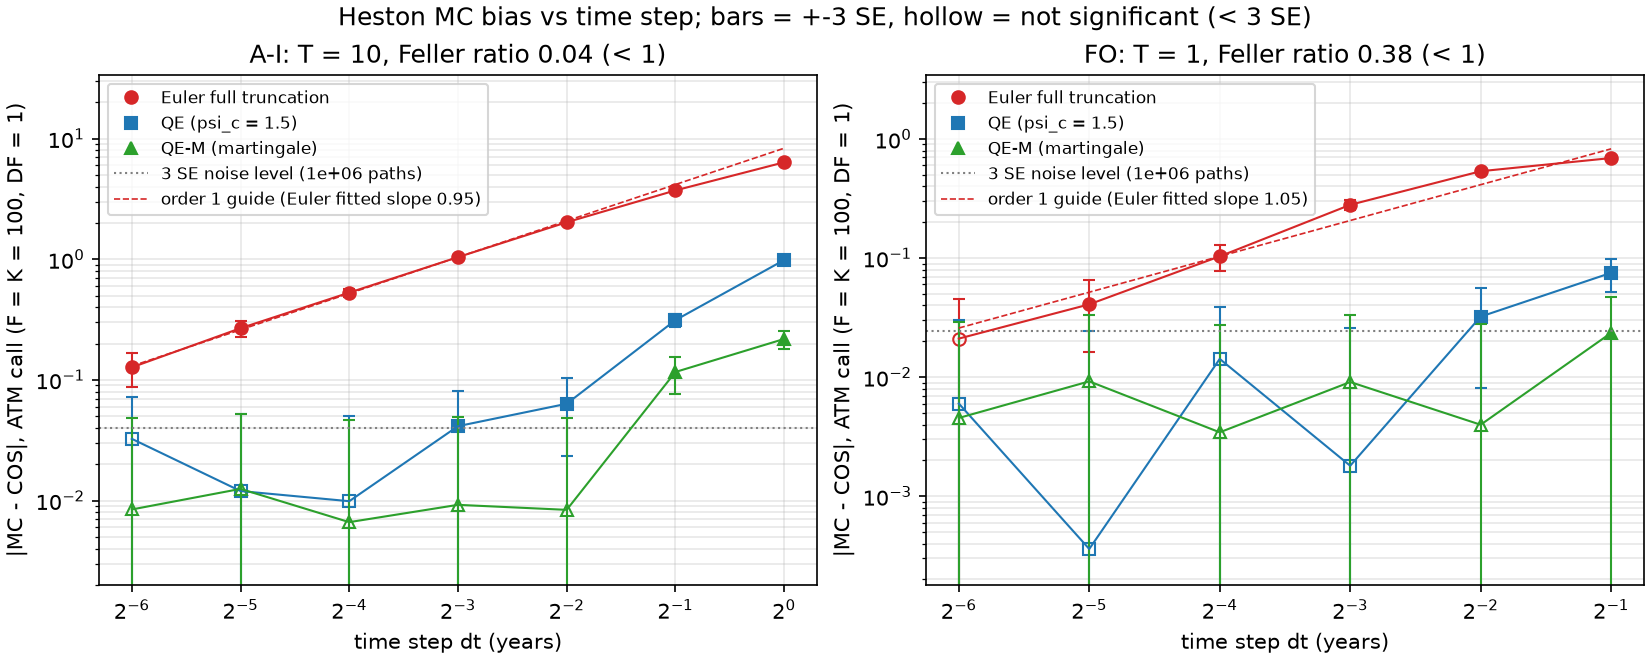
\includegraphics[width=\textwidth]{heston_euler_bias.png}
\caption{Heston Monte Carlo bias against the time step, ATM call ($F=K=100$, $\DF=1$), $10^6$ paths per point. Bars
$\pm3\,\SE$; open symbols mark non-significant points ($<3\,\SE$). Left: set A-I ($T=10$, $\nu_F=0.04$). Right: set
FO ($T=1$, $\nu_F=0.38$). The dashed red line is an order-1 guide.}
\label{fig:heston-euler-bias}
\end{figure}

Figure~\ref{fig:heston-euler-bias} shows the bias $|\text{MC}-\text{COS}|$ of the three schemes of this chapter
against $\Delta$, on a log-log scale.
\begin{itemize}
\item \textbf{Euler, set A-I} ($\nu_F=0.04$): $+6.368$ at $\Delta=1$, $+0.268$ at $\Delta=1/32$ (19.6~SE), $+0.127$
at $\Delta=1/64$. The decrease is monotonic and always significant; the estimated slope is 0.945.
\item \textbf{Euler, set FO}: $+0.692$ at $\Delta=\tfrac12$, $+0.041$ at $\Delta=1/32$ (5.0~SE), $+0.021$ at
$\Delta=1/64$ (2.6~SE, by now inside the noise). Estimated slope 1.054.
\item \textbf{QE and QE-M} (below) have much smaller biases already at coarse steps and drop into the noise much
earlier.
\end{itemize}
The acceptance criterion for the figure is: the Euler bias exceeds 3~SE at the coarsest step and decreases
monotonically until it enters the noise band. No slope is claimed inside the noise.

\begin{progetto}[title={In the qpricer project: comparison with the literature}]
Andersen publishes, for set A-I, $K=100$, the bias of Euler with full truncation: $+6.394$ at $\Delta=1$, $+1.051$ at
$\Delta=1/8$, $+0.243$ at $\Delta=1/32$. The project measures $+6.368$, $+1.042$, $+0.268$: the scheme is the same.

At the gate step ($\Delta=1/32$, ${2\times10^5}$ paths, puts with $K=70,100,140$) Euler on set A-I measures
$z=+4.39$, $+5.08$ and $+1.28$. This was predicted before running the test: at $K=100$ the published bias (0.243) is
larger than $3\,\SE\approx0.17$ (SE 0.058). This is why Euler is \emph{not} subjected to the 3~SE test: it is the
scheme, not a bug, and it goes into Figure~\ref{fig:heston-euler-bias}.
\end{progetto}

\section{Andersen's QE scheme}
\subsection{The idea}
Instead of taking an Euler step on the variance, we \emph{sample} $v_{n+1}$ from a simple distribution that has
exactly the same mean and variance as the true law (``quadratic--exponential'', QE).

\textbf{Step 1: the exact moments.} Conditional on $v_n$, the true law of $v_{n+1}$ is a scaled non-central
chi-squared. Its first two moments are, with $E=e^{-\kappa\Delta}$:
\begin{equation}\label{eq:qe-momenti}
m=\theta+(v_n-\theta)E,\qquad
s^2=\frac{v_n\xi^2E(1-E)}{\kappa}+\frac{\theta\xi^2(1-E)^2}{2\kappa}.
\end{equation}
Their relative dispersion is $\psi=s^2/m^2$. It is largest at $v_n=0$, where it equals $1/\nu_F$: the more Feller is
violated, the more dispersed the law of $v_{n+1}$ is relative to its mean.

\textbf{Step 2a ($\psi\le\psi_c$, variance away from zero): square of a Gaussian.} We set $v_{n+1}=a(b+Z_v)^2$. This
variable has mean $a(1+b^2)$ and variance $2a^2(1+2b^2)$. Imposing mean $m$ and variance $s^2$, with $y=b^2$:
\[
\psi(1+y)^2=2(1+2y)\iff y^2+2y\Big(1-\frac2\psi\Big)+1-\frac2\psi=0 .
\]
The non-negative root is
\begin{equation}\label{eq:qe-quad}
b^2=\frac2\psi-1+\sqrt{\frac2\psi}\sqrt{\frac2\psi-1},\qquad a=\frac{m}{1+b^2}.
\end{equation}
The discriminant is non-negative only if $\psi\le2$.

\textbf{Step 2b ($\psi>\psi_c$, variance near zero): atom at zero plus exponential.} With probability $p$ we set
$v_{n+1}=0$; otherwise we draw an exponential with parameter $\beta$. The mixture has mean $(1-p)/\beta$ and variance
$(1-p^2)/\beta^2$, hence $\psi=(1+p)/(1-p)$ and
\begin{equation}\label{eq:qe-exp}
p=\frac{\psi-1}{\psi+1},\qquad\beta=\frac{1-p}{m}.
\end{equation}
This requires $\psi\ge1$. We sample by inverting the distribution function with $U_v=\Phi(Z_v)$:
\[
v_{n+1}=\begin{cases}0 & U_v\le p,\\[2pt] \dfrac1\beta\ln\dfrac{1-p}{1-U_v} & U_v>p.\end{cases}
\]
The threshold $\psi_c$ must lie in $[1,2]$ for both branches to be defined; the project uses $\psi_c=1.5$, Andersen's
choice. If $\nu_F\ge2/3$ the exponential branch is never triggered.

\begin{perche}[title={Why QE is better than Euler}]
The two moments are exact at \emph{every} step and for any $\Delta$, because $m$ and $m^2+s^2$ are polynomials in
$v_n$ with exactly the coefficients of the CIR process. By the tower property, $\E\hat v_T$ and $\E\hat v_T^2$ are
exact as well.

The atom at zero reproduces the mass that the true process accumulates near zero when Feller is violated. Published
result (Andersen): QE with an annual or semi-annual step is as accurate as Euler with step $1/32$.
\end{perche}

\subsection{The log-forward step}
Integrating the variance equation over one step expresses the ``awkward'' stochastic integral in terms of known
quantities:
\[
\int_t^{t+\Delta}\!\sqrt{v_u}\dd W^v_u=\frac1\xi\Big(v_{t+\Delta}-v_t-\kappa\theta\Delta+\kappa I\Big),
\qquad I=\int_t^{t+\Delta}v_u\dd u .
\]
Writing $W^F=\rho W^v+\sqrt{1-\rho^2}\,W^\perp$, given the path of $v$ the $W^\perp$ term is Gaussian with variance
$(1-\rho^2)I$. Approximating $I\approx\tfrac\Delta2(v_n+v_{n+1})$ (trapezoidal rule) gives
\begin{equation}\label{eq:qe-x}
x_{n+1}=x_n+K_0+K_1v_n+K_2v_{n+1}+\sqrt{K_3v_n+K_4v_{n+1}}\;Z_\perp,
\end{equation}
with
\[
K_0=-\frac{\rho\kappa\theta\Delta}{\xi},\quad
K_{1,2}=\frac\Delta2\Big(\frac{\kappa\rho}{\xi}-\frac12\Big)\mp\frac\rho\xi,\quad
K_3=K_4=\frac\Delta2(1-\rho^2).
\]
The correlation enters only through $\frac\rho\xi(v_{n+1}-v_n)$: the leverage effect ``lives in the move of the
variance''. The normal $Z_\perp$ is independent of $Z_v$.

\begin{attenzione}
The naive alternative, Euler on the log-forward with a normal correlated with $Z_v$, ``loses'' correlation: $v_{n+1}$
depends on $Z_v$ non-linearly, and the linear correlation between the shocks is no longer $\rho$. The smile wings come
out too thin.
\end{attenzione}

\subsection{The martingale correction (QE-M)}
\label{sec:qe-m}
With the QE approximations, $\E[F_T]\ne F$: the simulated forward has a small drift. The reason is that the
continuous model satisfies an exact exponential identity on the joint law of $(v_{n+1},I)$. QE replaces $I$ with a
trapezoid and the law of $v_{n+1}$ with one that matches only in the first two moments. An exponential moment, on the
other hand, depends on the whole distribution, and the identity breaks at finite $\Delta$.

QE-M restores the martingale property step by step.

\textbf{Step 1.} Integrate out $Z_\perp$ with the Gaussian moment generating function:
\[
\E\big[e^{x_{n+1}-x_n}\mid v_n\big]=e^{K_0+(K_1+\frac12K_3)v_n}\;\E\big[e^{Av_{n+1}}\mid v_n\big],
\qquad A=K_2+\tfrac12K_4 .
\]
\textbf{Step 2.} $M(v_n)=\E[e^{Av_{n+1}}\mid v_n]$ is computed in closed form on each branch:
\begin{align*}
\text{quadratic branch:}\quad&\ln M=\frac{A\,b^2a}{1-2Aa}-\tfrac12\ln(1-2Aa)\qquad(\text{requires }2Aa<1),\\
\text{exponential branch:}\quad&M=p+\frac{\beta(1-p)}{\beta-A}\qquad(\text{requires }A<\beta).
\end{align*}
\textbf{Step 3.} Replace $K_0$, for every path and every step, with
\begin{equation}\label{eq:qe-m}
K_0^*(v_n)=-\ln M(v_n)-\big(K_1+\tfrac12K_3\big)v_n,
\end{equation}
so that $\E[e^{x_{n+1}-x_n}\mid v_n]=1$ exactly.

For $\rho\le0$ we have $A\le0$ (not every summand is negative, but their sum is), hence $2Aa<1$ and $A<\beta$ always
hold and $M$ is always defined (the SPX case). For $\rho>0$ the conditions restrict the step; the code checks every
path and raises an error instead of silently falling back to QE.

\begin{attenzione}[title={Two typos in the source}]
In the working-paper version of Andersen the exponential-branch formula is printed without the atom $p$, and the
expression for $K_0^*$ without the factor $v_n$. The sanity check $A=0\Rightarrow M=1$ exposes the first typo (the
printed formula would give $1-p$). The formulas above are checked against QuantLib and Choi--Kwok (2024).
\end{attenzione}

\begin{perche}[title={Why the martingale property matters}]
The forward is the hedging instrument. A scheme that misprices it breaks parity against the market, makes ITM prices
drift, and transfers its own error into any control variate based on $F_T$. Measured in the project on set A-I at
$\Delta=1$: $\overline{F_T}-F=+0.385$ (SE~0.035) with QE, $+0.009$ (SE~0.034) with QE-M.
\end{perche}

\section{Practical details}
\begin{itemize}
\item \textbf{Reproducibility.} A generator \code{np.random.Generator(seed)} is passed explicitly. At each step a
$(2,N)$ block is drawn (row 0 $=Z_v$, row 1 $=Z_\perp$), always in the same order in all schemes. Every MC kernel
returns \code{(price, SE, N, seed)}.
\item \textbf{Memory.} Storing all trajectories costs $N\times M\times8$ bytes (0.5\,GB for ${2\times10^5}$
trajectories and 320 steps). Only the current state and the quantities the payoff needs (minima, sums, observations)
are kept.
\item \textbf{Vectorized branches.} \code{np.where} evaluates \emph{both} branches on all paths: \code{NaN}s or
infinities may appear in the branch that is not selected. The quadratic branch is evaluated on $\min(\psi,\psi_c)$ and
the exponential one on $\max(\psi,\psi_c)$.
\item \textbf{Normal tails.} $1-U_v$ must be computed as $\Phi(-Z_v)$, not as $1-\Phi(Z_v)$: for $Z_v\gtrsim8.3$ the
latter is exactly 0 and would give $v_{n+1}=\infty$.
\item \textbf{A single $Z_v$ per step, in all branches.} This way, when a parameter is bumped and a path switches
branch, the random streams stay aligned (common random numbers).
\end{itemize}

\begin{progetto}[title={In the qpricer project: Heston Monte Carlo checks}]
Code: \code{src/qpricer/engines/mc.py} (\code{european\_price}, \code{simulate}, \code{heston\_steps}).
\begin{itemize}
\item \textbf{QE and QE-M against COS}: 24 comparisons. Sets FO, GS, BK-2 and A-I, all with Feller violated
($\nu_F=0.38,\ 0.62,\ 0.36,\ 0.04$); puts at $K\in\{70,100,140\}$; ${2\times10^5}$ trajectories; $\Delta=1/32$; seeds
fixed in advance. Result: 24 out of 24 within 3~SE, with $\max|z|=0.71$.
\item \textbf{Anti-selection check}: 20 fresh seeds declared in advance, same comparisons, 480 values of $z$. Maximum
$|z|=2.86$, none above 3; mean $-0.115$, standard deviation 0.937.
\item \textbf{Independent implementation}: a second implementation of QE-M, with a different ordering of the random
numbers, gives $\max|z|=1.35$ at the same settings.
\item \textbf{Martingale}: $\overline{F_T}=F$ within 3~SE for Euler and QE-M, including on sets never used before
($\rho=+0.5$, $\xi=1.5$, $\rho=-0.99$). Power check: plain QE, set FO, a single step, must fail: it measures
$+12.8$~SE.
\item \textbf{Two points at about 3~SE in the figure}, redone with ${4\times10^6}$ paths. QE on A-I at $\Delta=1/8$
($-3.1$~SE) was noise: $-0.0031$ (SE~0.0067). QE-M on FO at $\Delta=\tfrac12$ ($-3.0$~SE) is a genuine coarse-step
bias of the scheme: $-0.0236$ (SE~0.0039). Neither concerns the gate at $\Delta=1/32$.
\item \textbf{Limit $\xi\to0$}: each scheme converges to Black with its own \emph{discrete} integrated variance (which
can be computed exactly), which in turn converges to $\bar\Sigma$ as $\Delta\to0$.
\end{itemize}
\end{progetto}

\begin{riassunto}
\begin{itemize}
\item $\hat V=\DF\,\bar g$, $\SE=\DF\,s_g/\sqrt N$; error $\propto N^{-1/2}$; finite variance is required, hence we
simulate puts.
\item 3~SE test: 0.27\% false alarms per test; with $m$ tests $1-0.9973^m$; power only for biases $\gtrsim3\,\SE$;
seeds fixed and declared in advance.
\item Bias (from $\Delta$) and noise (from $N$) are different errors; halving $\Delta$ means quadrupling $N$.
\item With CRN, a 3~SE test on step halving fails for an order-1 scheme: it is replaced by a size check and an order
check.
\item Heston: Euler produces negative variances; full truncation is the least distorting fix and preserves the
martingale property, but has a large order-1 bias when Feller is violated. QE samples the variance with exact mean and
variance; QE-M restores the martingale property.
\end{itemize}
\end{riassunto}

\begin{domande}
\begin{enumerate}
\item How is the standard error of an MC price computed? How does it scale with $N$?
\item You run 100 tests at 3~SE and one fails: is there a bug in the code? What do you do?
\item Why does a passed test not prove that the scheme is unbiased?
\item Why does a 3~SE test on step halving, with common random numbers, fail for a correct order-1 scheme? What do
you replace it with?
\item Why does full truncation distort less than absorption and reflection?
\item How does QE choose the distribution of $v_{n+1}$? Why are there two branches, and why $\psi_c\in[1,2]$?
\item Why is plain QE not a martingale, and how does QE-M restore the property?
\item Why is it better to simulate puts rather than calls in Heston and SABR?
\end{enumerate}
\end{domande}

\chapter{The SABR model}
\label{cap:sabr}

Heston describes the \emph{whole} surface with five parameters. SABR (Hagan, Kumar, Lesniewski and Woodward, 2002)
makes a different choice: it describes \emph{one smile at a time} (one expiry) with three nearly independent
parameters and, above all, it provides an \textbf{approximate implied volatility formula} that is computed
instantly. It is the market standard in interest rates and is also useful in equities for interpolating smiles.

Hagan's formula, however, is an \emph{asymptotic expansion}, not the model. This chapter derives the formula,
checks it against two Monte Carlo simulations of the true model, and measures where it stops being valid.

\section{The dynamics}
\begin{equation}\label{eq:sabr}
\dd F_t=\alpha_tF_t^\beta\dd W_t,\qquad\dd\alpha_t=\nu\,\alpha_t\dd Z_t,\qquad\dd\langle W,Z\rangle_t=\rho\dd t .
\end{equation}
Here $\alpha_t$ is a lognormal stochastic volatility without mean reversion, with initial value $\alpha$; $\nu\ge0$ is
its volatility (vol-of-vol), per $\sqrt{\text{year}}$; $\rho$ is the correlation between forward and volatility;
$\beta\in[0,1]$ is the ``elasticity exponent''.

\subsection{\texorpdfstring{Why $\beta=1$ for the SPX}{Why β=1 for the SPX}}
\begin{perche}
\begin{itemize}
\item \textbf{$\beta$ is not identifiable from a smile.} Both $\beta$ and $\rho$ produce slope: the ATM slope is
about $-\tfrac12(1-\beta)\sigma_{\mathrm{ATM}}+\tfrac12\rho\nu$. Moreover, the level
$\sigma_{\mathrm{ATM}}\approx\alpha F^{\beta-1}$ makes $\alpha$ trade off against $\beta$. With $\beta$ free the
$(\alpha,\beta,\rho)$ calibration is ill-conditioned; Hagan et al.\ themselves write that estimating $\beta$ from the
smile amounts to ``fitting the noise''.
\item \textbf{$\beta$ is a choice of dynamics, not of price.} It decides how the ATM volatility moves when the forward
moves (the \emph{backbone}): it changes the deltas, not today's prices.
\item \textbf{$\beta=1$ is natural for an equity index.} The model is lognormal and \emph{scale-free}: the volatility
depends only on $K/F$, $\alpha$ is directly a volatility, and all the price--volatility co-movement sits in $\rho$.
\item \textbf{It is numerically convenient.} No boundary at $F=0$, positive and martingale simulation, ATM inversion
via a quadratic equation.
\end{itemize}
\end{perche}

With $\beta=1$, by Itô and the explicit solution of geometric Brownian motion:
\begin{equation}\label{eq:sabr-beta1}
\dd\ln F_t=-\tfrac12\alpha_t^2\dd t+\alpha_t\dd W_t,\qquad \alpha_t=\alpha\,e^{\nu Z_t-\nu^2t/2}\quad\text{(exact)}.
\end{equation}

\subsection{Model facts that matter}
For $\beta=1$ two results of Lions and Musiela (2007) hold.
\begin{itemize}
\item \textbf{Martingale.} $F$ is a true martingale if and only if $\rho\le0$. For $\rho>0$ it is a strict local
martingale: $\E F_T<F$.
\item \textbf{Moments.} For $m>1$, $\E F_T^m<\infty$ if and only if $\rho\le-\sqrt{(m-1)/m}$. In particular
$\Var F_T<\infty$ only if $\rho\le-1/\sqrt2\approx-0.71$. At $\rho=0$ all moments of order $>1$ are infinite.
\end{itemize}
\begin{attenzione}
Practical consequence: the call payoff can have infinite variance, so the standard error of an MC estimate on calls is
not reliable. We simulate \textbf{puts} (payoff bounded by $K$). Calls are obtained by parity with $F$, but only for
$\rho\le0$ (Section~\ref{sec:sabr-rho-pos}).
\end{attenzione}

\section{\texorpdfstring{Hagan's formula ($\beta=1$)}{Hagan's formula (β=1)}}
With $k=\ln(K/F)$:
\begin{equation}\label{eq:hagan}
\boxed{\sigma_H(K)=\alpha\,\frac{z}{x(z)}\,\big(1+c_1T\big)},\qquad z=\frac\nu\alpha\ln\frac FK=-\frac{\nu k}{\alpha},\qquad
c_1=\frac{\rho\nu\alpha}4+\frac{2-3\rho^2}{24}\nu^2,
\end{equation}
\begin{equation}\label{eq:hagan-x}
x(z)=\ln\frac{D(z)+z-\rho}{1-\rho}=\int_0^z\frac{\dd u}{D(u)},\qquad D(z)=\sqrt{1-2\rho z+z^2}.
\end{equation}
The price is obtained by plugging $\sigma_H(K)$ into the Black formula \eqref{eq:black}:
\[
V=\mathrm{Black}\big(F,K,T,\DF,\sigma_H(K)\big).
\]

\subsection{\texorpdfstring{Where the factor $z/x(z)$ comes from}{Where the factor z/x(z) comes from}}
\noindent\textbf{Step 1.} Measure the distance to the strike in units of the current volatility:
$u_t=\ln(F_t/K)/\alpha_t$.

\noindent\textbf{Step 2.} By Itô, neglecting the $\dd t$ terms, $\dd u=\dd W-\nu u\,\dd Z$. Its ``diffusion speed''
is
\[
\frac{\dd\langle u\rangle}{\dd t}=1-2\rho\nu u+\nu^2u^2=D(\nu u)^2 .
\]
This is the only place where $\rho$ and $\nu$ enter at leading order.

\noindent\textbf{Step 3.} For short times the probability of reaching the strike decays like $e^{-\delta^2/2T}$,
where $\delta$ is the distance measured with this variable speed:
\[
\delta=\int_0^{u_0}\frac{\dd u}{D(\nu u)}=\frac{x(z)}{\nu},\qquad z=\nu u_0 .
\]
\noindent\textbf{Step 4.} In Black with volatility $\sigma$ the same distance is $\ln(F/K)/\sigma$. Equating the two
distances:
\[
\sigma=\frac{\nu\ln(F/K)}{x(z)}=\alpha\,\frac{z}{x(z)} .
\]
As $K\to F$ we have $z/x\to1$.

\begin{idea}
The implied volatility at a strike is, approximately, the volatility ``seen'' along the most likely path to that
strike. With $\rho<0$, moving down towards low strikes means that volatility rises: hence the skew. The vol-of-vol
makes both wings expensive, because large moves happen in high-volatility states.
\end{idea}

\subsection{\texorpdfstring{The factor $(1+c_1T)$: a check at $\rho=0$}{The factor (1+c₁T): a check at ρ=0}}
The factor $(1+c_1T)$ is the first correction in $T$; its full derivation is in the appendix of Hagan et al. The
$\rho=0$ part, however, can be checked by hand.

\noindent\textbf{Step 1.} At $\rho=0$, given the path of $\alpha$, $\ln F_T$ is Gaussian with variance
$I=\int_0^T\alpha_t^2\dd t$. The price is the average of Black prices, and ATM Black is linear in $\sqrt I$ at first
order. Hence $\sigma_{\mathrm{ATM}}\approx\E\sqrt{I/T}$.

\noindent\textbf{Step 2.} Write $I/(\alpha^2T)=1+\epsilon$ with $\E\epsilon=\nu^2T/2+O(\nu^3)$ and
$\E\epsilon^2=4\nu^2T/3+O(\nu^3)$ (from the expansion of $e^{2\nu Z_t-\nu^2t}$ and the moments of Brownian motion).

\noindent\textbf{Step 3.} With $\sqrt{1+\epsilon}\approx1+\tfrac12\epsilon-\tfrac18\epsilon^2$:
\[
\E\sqrt{1+\epsilon}\approx1+\frac{\nu^2T}{4}-\frac{\nu^2T}{6}=1+\frac{2\nu^2T}{24},
\]
which is exactly $c_1T$ at $\rho=0$.

\subsection{Near the money: three nearly orthogonal knobs}
Expanding for small $k$:
\begin{equation}\label{eq:sabr-taylor}
\sigma_H\approx(1+c_1T)\Big[\alpha+\tfrac12\rho\nu\,k+\frac{(2-3\rho^2)\nu^2}{12\alpha}k^2\Big].
\end{equation}
\begin{itemize}
\item $\alpha$ sets the \textbf{level};
\item $\rho\nu$ sets the \textbf{slope}: ATM skew $=\tfrac12\rho\nu(1+c_1T)$;
\item $\nu^2/\alpha$ sets the \textbf{curvature}.
\end{itemize}
This also gives good starting values for the calibration: fit a parabola $\sigma_0+Sk+\tfrac12Ck^2$ to the
near-the-money data and invert the relations.

\section{\texorpdfstring{The ATM inversion for $\alpha$}{The ATM inversion for α}}
\subsection{The quadratic equation}
As $K\to F$, $\sigma_{\mathrm{ATM}}=\alpha(1+c_1T)$. Substituting $c_1$:
\[
\sigma_{\mathrm{ATM}}=\alpha\Big(1+\frac{(2-3\rho^2)\nu^2T}{24}\Big)+\alpha^2\,\frac{\rho\nu T}{4}.
\]
Given the market $\sigma_{\mathrm{ATM}}$, $\alpha$ therefore solves
\begin{equation}\label{eq:alpha-atm}
a\alpha^2+b\alpha-\sigma_{\mathrm{ATM}}=0,\qquad a=\frac{\rho\nu T}{4},\qquad b=1+\frac{(2-3\rho^2)\nu^2T}{24}.
\end{equation}
With $\beta<1$ it would be a cubic equation; $\beta=1$ removes the $\alpha^3$ term.

\subsection{Which root, and in what form}
The textbook formula $(-b+\sqrt{b^2+4a\sigma_{\mathrm{ATM}}})/(2a)$ suffers cancellation as $a\to0$ (that is,
$\rho\nu\to0$). Rationalizing gives the stable form
\begin{equation}\label{eq:alpha-stabile}
\alpha=\frac{2\sigma_{\mathrm{ATM}}}{b+\sqrt{b^2+4a\sigma_{\mathrm{ATM}}}},
\end{equation}
which tends to $\sigma_{\mathrm{ATM}}/b$ as $a\to0$ with no division by zero.

It is the \emph{small} root, the one for which the correction $(1+c_1T)$ stays $\ge b/2$. On the other root the
``correction'' would dominate the leading term, and the expansion would make no sense. For $\rho>0$ the product of
the roots is $-\sigma_{\mathrm{ATM}}/a<0$: there is exactly one positive root.

\subsection{\texorpdfstring{The feasibility ceiling for $\rho<0$}{The feasibility ceiling for ρ<0}}
For $\rho<0$ we have $a<0$, and the function $\alpha\mapsto\sigma_{\mathrm{ATM}}(\alpha)=\alpha(b+a\alpha)$ is a
downward-opening parabola. It has a maximum at the vertex $\alpha^*=b/(2|a|)$, where it equals
\begin{equation}\label{eq:tetto}
\sigma_{\mathrm{ATM}}^{\max}=\frac{b^2}{4|a|}.
\end{equation}
Above this ceiling the discriminant is negative: \emph{no} $\alpha$ reproduces the given ATM volatility.

\begin{esempio}[title={Example: the ceiling at $\rho=-0.9$, $\nu=2$, $T=5$}]
\begin{itemize}
\item $a=\rho\nu T/4=-0.9\cdot2\cdot5/4=-2.25$.
\item $b=1+(2-3\cdot0.81)\cdot4\cdot5/24=1-0.43\cdot20/24\approx0.642$.
\item $\sigma_{\mathrm{ATM}}^{\max}=b^2/(4|a|)\approx0.412/9\approx0.0457$.
\end{itemize}
With these $(\rho,\nu)$ no ATM volatility above 4.57\% is attainable. At $\rho=-0.9$, $\nu=5$, $T=2$ the ceiling drops
to about 0.12\%, and these parameters lie within the plausible bounds of a calibration.
\end{esempio}

\begin{progetto}[title={In the qpricer project: ATM inversion}]
\code{alpha\_from\_atm} in \code{src/qpricer/models/sabr.py} uses \eqref{eq:alpha-stabile}. Above the ceiling it
returns \code{NaN} with a warning, never a clipped value. An independent check confirmed that this happens exactly
when no positive root exists (20{,}000 points), and that the root agrees with a numerical search on $[0,\alpha^*]$ to
within $10^{-13}$. The round trip $\sigma_{\mathrm{ATM}}(\hat\alpha)=\sigma_{\mathrm{ATM}}$ is exact to
$4.4\times10^{-16}$ wherever $b>0$, that is, for every $\rho\le0$.

\smallskip
In calibration (Chapter~\ref{cap:calibrazione}) the objective function uses $(\alpha,\rho,\nu)$ directly, and
\eqref{eq:alpha-stabile} serves only to build the starting points. Points without a positive root are discarded and
counted: 0 out of 195 across the 39 expiries.
\end{progetto}

\section{Evaluating the formula without losing digits}
\subsection{\texorpdfstring{The limit $z\to0$}{The limit z→0}}
For $K=F$ or $\nu=0$ we have $z=0$ and $z/x(z)$ is $0/0$. For $|z|<z_c=10^{-3}$ the series expansion is used:
\begin{equation}\label{eq:zx-serie}
\frac z{x(z)}=1-\frac{\rho z}2+\frac{(2-3\rho^2)z^2}{12}+\frac{\rho(5-6\rho^2)z^3}{24}+O(z^4).
\end{equation}
It is obtained by integrating the generating function of the Legendre polynomials, $1/D(u)=\sum_nP_n(\rho)u^n$, and
inverting the series. The coefficient of $z^4$ is at most 0.05 in absolute value, so at $z_c$ the series error is
$\le5\times10^{-14}$.

\subsection{Branching on sign, and \code{log1p}}
For $|z|\ge z_c$ we use \eqref{eq:hagan-x}, with two precautions.

\noindent\textbf{Step 1: no cancellation as $\rho\to\pm1$.} Write $D^2=(z-\rho)^2+(1-\rho)(1+\rho)$, a sum of
non-negative terms. For $z<\rho$ and $\rho$ close to $\pm1$ we have $D\approx\rho-z$, and $D+z-\rho$ cancels; we then
use the identity $(D+z-\rho)(D-z+\rho)=1-\rho^2$, which gives
\[
x(z)=\ln\frac{1+\rho}{D+\rho-z}\qquad(z<\rho).
\]
\noindent\textbf{Step 2: no loss of digits for small $z$.} For small $z$ the argument of the logarithm is $1+O(z)$,
and the direct logarithm has a relative error of about $4\varepsilon/|z|$ (with $\varepsilon=2^{-52}$). Instead,
``argument minus 1'' is computed exactly with the identity
\[
D-1=\frac{D^2-1}{D+1}=\frac{z(z-2\rho)}{D+1},
\]
and passed to \code{log1p}:
\begin{align*}
x&=\mathrm{log1p}\Big(\frac{z\,(D+1+z-2\rho)}{(D+1)(1-\rho)}\Big) &&\text{for } z\ge\rho,\\
x&=-\mathrm{log1p}\Big(-\frac{z\,(D+1+2\rho-z)}{(D+1)(1+\rho)}\Big) &&\text{for } z<\rho.
\end{align*}
The relative error is now $O(\varepsilon)$ for every $z$.

\subsection{Non-positive volatility}
If $c_1<0$ (for example with $|\rho|>\sqrt{2/3}$), for $T\ge1/|c_1|$ the factor $1+c_1T$ is $\le0$ and the formula
returns a non-positive volatility. The code returns \code{NaN} with a warning; it never clips.

\begin{progetto}[title={In the qpricer project: checks of the formula}]
\code{z\_over\_x} and \code{implied\_vol} in \code{src/qpricer/models/sabr.py}.
\begin{itemize}
\item Against a transcription of Hagan in 60-digit decimal arithmetic, on 1500 random points ($\alpha,\nu\le5$,
$|\rho|\le0.999$, $T\le30$, $|k|\le3$): relative error $5.0\times10^{-14}$.
\item Jump across $|z|=z_c$, net of the true slope: $4.7\times10^{-14}$ relative.
\item Symmetry at $\rho=0$, $\sigma(k)=\sigma(-k)$: $4.4\times10^{-16}$.
\item $x(z)$ against quadrature of $\int_0^z\dd u/D(u)$, including at $\rho=\pm0.999$: $2.9\times10^{-15}$.
\item Limit $\nu\to0$ (gate, threshold $10^{-10}$, $|k|\le1$, $T$ from 0.01 to 10, six values of $\rho$): at $\nu=0$
the gap from $\alpha$ is exactly 0; at $\nu=10^{-12}$ it is $3.0\times10^{-12}$.
\end{itemize}
\end{progetto}

\section{\texorpdfstring{SABR Monte Carlo ($\beta=1$)}{SABR Monte Carlo (β=1)}}
\subsection{Log-Euler with exact volatility}
On a grid $t_n=n\Delta$, with $Z_F=\rho Z_\alpha+\sqrt{1-\rho^2}Z_\perp$:
\begin{align}
\alpha_{n+1}&=\alpha_n\exp\big(\nu\sqrt\Delta Z_{\alpha,n}-\tfrac12\nu^2\Delta\big),\label{eq:sabr-alpha}\\
\ln F_{n+1}&=\ln F_n-\tfrac12\alpha_n^2\Delta+\alpha_n\sqrt\Delta\, Z_{F,n}.\label{eq:sabr-euler}
\end{align}
Properties:
\begin{itemize}
\item $\hat\alpha$ is exact in law on the grid ($\ln\alpha$ is a Brownian motion with drift);
\item $\hat F>0$ always;
\item $\E[\hat F_{n+1}\mid\mathcal F_{t_n}]=\hat F_n$ exactly, for every $\Delta$ and every $\rho$, by the same
argument used for Euler in Heston (Chapter~\ref{cap:mc}).
\end{itemize}
The only error comes from the integrated variance $I=\int\alpha^2\dd t$, approximated with the left-point rule, and
from the correlation term. The scheme has weak order 1.

\begin{perche}[title={How biased is the integrated variance?}]
\noindent\textbf{Step 1.} $\E\alpha_t^2=\alpha^2e^{\nu^2t}$.

\noindent\textbf{Step 2.} The left sum is a geometric series:
\[
\E\hat I=\Delta\sum_{n=0}^{M-1}\alpha^2e^{\nu^2n\Delta}=\alpha^2\Delta\,\frac{e^{\nu^2T}-1}{e^{\nu^2\Delta}-1},
\qquad\E I=\alpha^2\,\frac{e^{\nu^2T}-1}{\nu^2}.
\]
\noindent\textbf{Step 3.} The ratio is
\[
\frac{\E\hat I}{\E I}=\frac{\nu^2\Delta}{e^{\nu^2\Delta}-1}=1-\tfrac12\nu^2\Delta+O(\Delta^2).
\]
The variance is too small by about $\tfrac12\nu^2\Delta$, and the ATM volatility comes out low by about
$\alpha\nu^2\Delta/4$. With $\alpha=0.2$, $\nu=0.4$, $\Delta=1/250$ this is about 0.003 vol points, against a standard
error of about 0.065 vol points at $N=2\times10^5$ (hand estimates).
\end{perche}

\begin{attenzione}
One cannot ``improve'' the integrated variance by putting the trapezoidal rule only in the drift of
\eqref{eq:sabr-euler}: with $\rho\ne0$ this would break the martingale property. For a higher order, a different
estimator is used: the conditional one.
\end{attenzione}

\subsection{The conditional (mixing) estimator}
Given the path of $\alpha$, the log-forward is Gaussian.

\noindent\textbf{Step 1.} From \eqref{eq:sabr}, $\int_0^T\alpha_t\dd Z_t=(\alpha_T-\alpha)/\nu$.

\noindent\textbf{Step 2.} Writing $W=\rho Z+\sqrt{1-\rho^2}Z^\perp$, given the path of $\alpha$ the $Z^\perp$ term is
Gaussian with variance $(1-\rho^2)I$:
\begin{equation}\label{eq:sabr-mixing}
\ln F_T=\ln F+\frac\rho\nu(\alpha_T-\alpha)-\tfrac12I+\sqrt{(1-\rho^2)I}\;Z .
\end{equation}
\noindent\textbf{Step 3.} The payoff is replaced by its conditional expectation, which is a Black price:
\begin{equation}\label{eq:sabr-mixing-stima}
\begin{aligned}
\hat V&=\DF\cdot\frac1N\sum_i\mathrm{Black}\Big(F\xi_i,\,K,\,\sqrt{(1-\rho^2)\hat I_i/T}\Big),\\
\xi_i&=\exp\Big\{\frac\rho\nu(\alpha_{T,i}-\alpha)-\tfrac12\rho^2\hat I_i\Big\},
\end{aligned}
\end{equation}
with $\hat I$ computed with the trapezoidal rule.

The noise of $Z^\perp$ is integrated out, and the bias is $O(\Delta^2)$. It is a second MC, independent of
log-Euler.

\begin{progetto}[title={In the qpricer project: numerical details of the MC}]
\code{sabr.simulate} and \code{sabr.mc\_price} (methods \code{"euler"} and \code{"mixing"}).
\begin{itemize}
\item $\alpha_n$ is rebuilt in closed form from the cumulated Brownian motion, so it is exact on the grid.
\item $(\alpha_T-\alpha)/\nu$ is computed as $\alpha\,\mathrm{expm1}(\nu W_T-\nu^2T/2)/\nu$, which tends to
$\alpha W_T$ as $\nu\to0$ without any thresholds.
\item Black is evaluated in $\ln(F\xi)$, because $F\xi$ underflows at large $\nu^2T$.
\item For $\rho\le0$ the conditional call is a bounded payoff, so the degradation figure prices OTM options (puts for
$k\le0$, calls for $k>0$) with the conditional estimator.
\end{itemize}
\end{progetto}

\section{The ``Hagan versus MC'' gate}
\subsection{Why in price space, and on puts}
The comparison is
\[
|\hat P_{\text{MC}}-P_{\text{Black}}(\sigma_H)|\le3\,\SE_P,
\]
with puts at every strike.
\begin{itemize}
\item \textbf{Puts}: bounded payoff, finite variance, reliable SE (the call can have infinite variance).
\item \textbf{Price, not volatility}: the Hagan side is deterministic, so all the noise is in the SE. Inverting a noisy
MC price into a volatility is a non-linear operation and can fail in the wings (the noisy price may fall outside the
no-arbitrage bounds). Volatilities are used only in the figure, with bars $\SE_P/\vega$.
\end{itemize}

\subsection{Set-up}
\begin{itemize}
\item Set G: $F=100$, $\DF=1$, $\alpha=0.2$, $\rho=-0.75$, $\nu=0.4$.
\item $T\in\{0.25,0.5,1\}$ and $k\in\{0,\pm0.05,\pm0.1,\pm0.2\}$: 21 comparisons, with $\nu^2T\le0.16$.
\item $N=2\times10^5$, \textbf{250 steps at every expiry} ($\Delta=T/250$), seeds fixed in advance.
\end{itemize}

\begin{perche}[title={Why 250 steps at every expiry, and not $\Delta=1/250$}]
The bias estimate $\alpha\nu^2\Delta/4$ holds ATM. In the wings the correlation term also matters, and the bias is
larger. An independent check showed that with a fixed step of $1/250$ (only 63 steps at $T=0.25$) the bias size check
failed at short expiries, whereas it had only been run at $T=1$. The fix was to use 250 steps at every expiry; the
tolerance did not change.
\end{perche}

\subsection{Results}
\begin{progetto}[title={In the qpricer project: the gate on set G}]
\begin{itemize}
\item Log-Euler, 21 comparisons: $\max|z|=1.68$ (threshold 3). The conditional estimator, reported alongside:
$\max|z|=2.77$.
\item The two MCs against each other, independent seeds, $T=1$: $|z|\le1.23$.
\item Independent checks: an MC written from scratch gives $\max|z|=2.42$. The expected (noise-free) gap between the
exact mean of the scheme and Hagan is at most 1.15 SE.
\end{itemize}
\smallskip
\noindent\textbf{Robustness over 100 fresh seeds} (21 comparisons each): 4.0\% of the seeds fail; per single
comparison 0.29\%; mean of the $z$ values $-0.074$, standard deviation 1.042. An independent check on another 100
seeds gives 5.0\%, consistent within the binomial error.
\end{progetto}

The 4.0\% does not match the $1-0.9973^{21}\approx5.5\%$ of the formula for independent tests, for two reasons
(Chapter~\ref{cap:mc}):
\begin{itemize}
\item the 21 comparisons use the same paths, so they are correlated;
\item there is a deterministic offset, mainly the error of Hagan itself in the left wing. At $T=1$, $k=-0.2$ the true
Hagan error is $+0.058$ vol points (ATM only $0.008$), about 1 SE: the mean of the $z$ values at that point is
$-1.05$.
\end{itemize}

\subsection{The step-halving test}
Chapter~\ref{cap:mc} (Section~\ref{sec:halving}) explains why a 3 SE test on the difference
$d=\hat V_\Delta-\hat V_{\Delta/2}$ with common random numbers cannot work for an order-1 scheme.
Table~\ref{tab:sabr-halving} reports the numbers, with $\Delta=T/250$ against $T/500$.

\begin{table}[htbp]
\centering
\small
\caption{Step halving on set G ($\Delta=T/250$ against $T/500$).}
\label{tab:sabr-halving}
\begin{tabular*}{\textwidth}{@{\extracolsep{\fill}}lccc@{}}
\toprule
 & $T=0.25$ & $T=0.5$ & $T=1$\\
\midrule
conditional: $|d|/\SE_d$ (must be $\le3$) & $\le1.60$ & $\le0.72$ & $\le0.51$\\
log-Euler: $d/\SE_d$ & $-7.96\ldots+2.46$ & $-5.13\ldots+3.77$ & $-4.79\ldots+1.48$\\
log-Euler: $\max|d|/\SE_{\text{gate}}$ (must be $\le0.1$) & 0.080 & 0.063 & 0.073\\
log-Euler: bias at $k=-0.2$ (vol points) & $-0.0104$ & $-0.0073$ & $-0.0084$\\
\bottomrule
\end{tabular*}
\end{table}

\begin{itemize}
\item The conditional estimator, of order 2, passes the 3 SE test as an identity.
\item Log-Euler fails it (down to $-7.96$), but passes the size check at all expiries. The Richardson bias $2d$ is
$\le0.17\,\SE_{\text{gate}}$ everywhere. An independent check, which computes the exact mean of the scheme, gives
$-0.0107$, $-0.0098$, $-0.0081$ vol points at $k=-0.2$ ($-0.164$, $-0.169$, $-0.139\,\SE_{\text{gate}}$).
\item Order check at $T=1$, $k=-0.2$: $M(\hat V_{1/M}-\hat V_{1/2M})=-0.25,\ -0.28,\ -0.31,\ -0.26$ for
$M=25,50,125,250$. It is flat within the noise: the scheme is of order 1 by construction; this is not a code error.
\end{itemize}

\subsection{A check against published values}
Choi, Hu and Kwok report finite-difference reference prices ($\beta=1$, $\alpha=0.2$, $T=1$, $F=K=1$, ATM call). They
are a single source: they serve as diagnostics, not as a gate (Table~\ref{tab:sabr-chk}).

\begin{table}[htbp]
\centering
\small
\caption{SABR ATM call ($\beta=1$, $\alpha=0.2$, $T=1$, $F=K=1$): values published by Choi, Hu and Kwok against
Hagan and against the conditional MC.}
\label{tab:sabr-chk}
\begin{tabular*}{\textwidth}{@{\extracolsep{\fill}}lcccr@{}}
\toprule
$(\rho,\nu)$ & published & Hagan $-$ published & conditional MC & $z$ MC vs published\\
\midrule
$(-0.75,\,0.2)$ & 0.07910 & $+1.6\times10^{-6}$ & $0.07908\pm0.00019$ & $-0.10$\\
$(-0.50,\,0.2)$ & 0.07942 & $+4.1\times10^{-6}$ & $0.07934\pm0.00013$ & $-0.66$\\
$(-0.25,\,0.2)$ & 0.07969 & $+7.0\times10^{-6}$ & $0.07977\pm0.00007$ & $+1.06$\\
$(-0.75,\,0.4)$ & 0.07860 & $+3.0\times10^{-5}$ & $0.07892\pm0.00021$ & $+1.55$\\
$(-0.75,\,0.6)$ & 0.07811 & $+1.3\times10^{-4}$ & $0.07805\pm0.00023$ & $-0.27$\\
\bottomrule
\end{tabular*}
\end{table}

The Hagan error grows with $\nu$, as expected. On the last row two independent methods (a quasi-random MC and a
partial differential equation) agree on 0.0781203: the published value is off by about $1.0\times10^{-5}$, twice its
rounding.

\section{Where the formula stops working}
\subsection{\texorpdfstring{The small parameter is $\nu^2T$}{The small parameter is ν²T}}
The formula is an expansion for ``small'' volatility and vol-of-vol over the life of the option. With $\beta=1$ the
prices depend only on $(k,\ \alpha\sqrt T,\ \nu\sqrt T,\ \rho)$, so the small parameters are $\nu^2T$, $\alpha^2T$
and $\rho\nu\alpha T$. The term $c_1T$ is the first correction; the neglected terms are of order $(\nu^2T)^2$.

\paragraph{The wings and Lee's bound.} As $|k|\to\infty$ we have $x(z)\approx\pm\ln\big(2|z|/(1\mp\rho)\big)$, hence
\[
\sigma_H\approx(1+c_1T)\,\frac{\nu|k|}{\ln\big(2\nu|k|/(\alpha(1\mp\rho))\big)},\qquad
\frac{\sigma_H^2T}{|k|}\to\infty .
\]
Absence of arbitrage (Lee's moment formula), however, requires $\limsup\sigma^2T/|k|\le2$. Far enough into the wings
the formula therefore implies \emph{negative} densities (butterfly arbitrage), and the problem moves closer to the
money as $\nu^2T$ grows.

\paragraph{Symmetry.} At $\rho=0$ the smile is symmetric in $k$, both in the model and in the formula. For
$\rho\ne0$ the symmetry $\rho\to-\rho$, $K\leftrightarrow F^2/K$ does \emph{not} hold: under the share measure the
volatility acquires a drift $\rho\nu\alpha^2$.

\subsection{The degradation figure}
\begin{figure}[htbp]
\centering
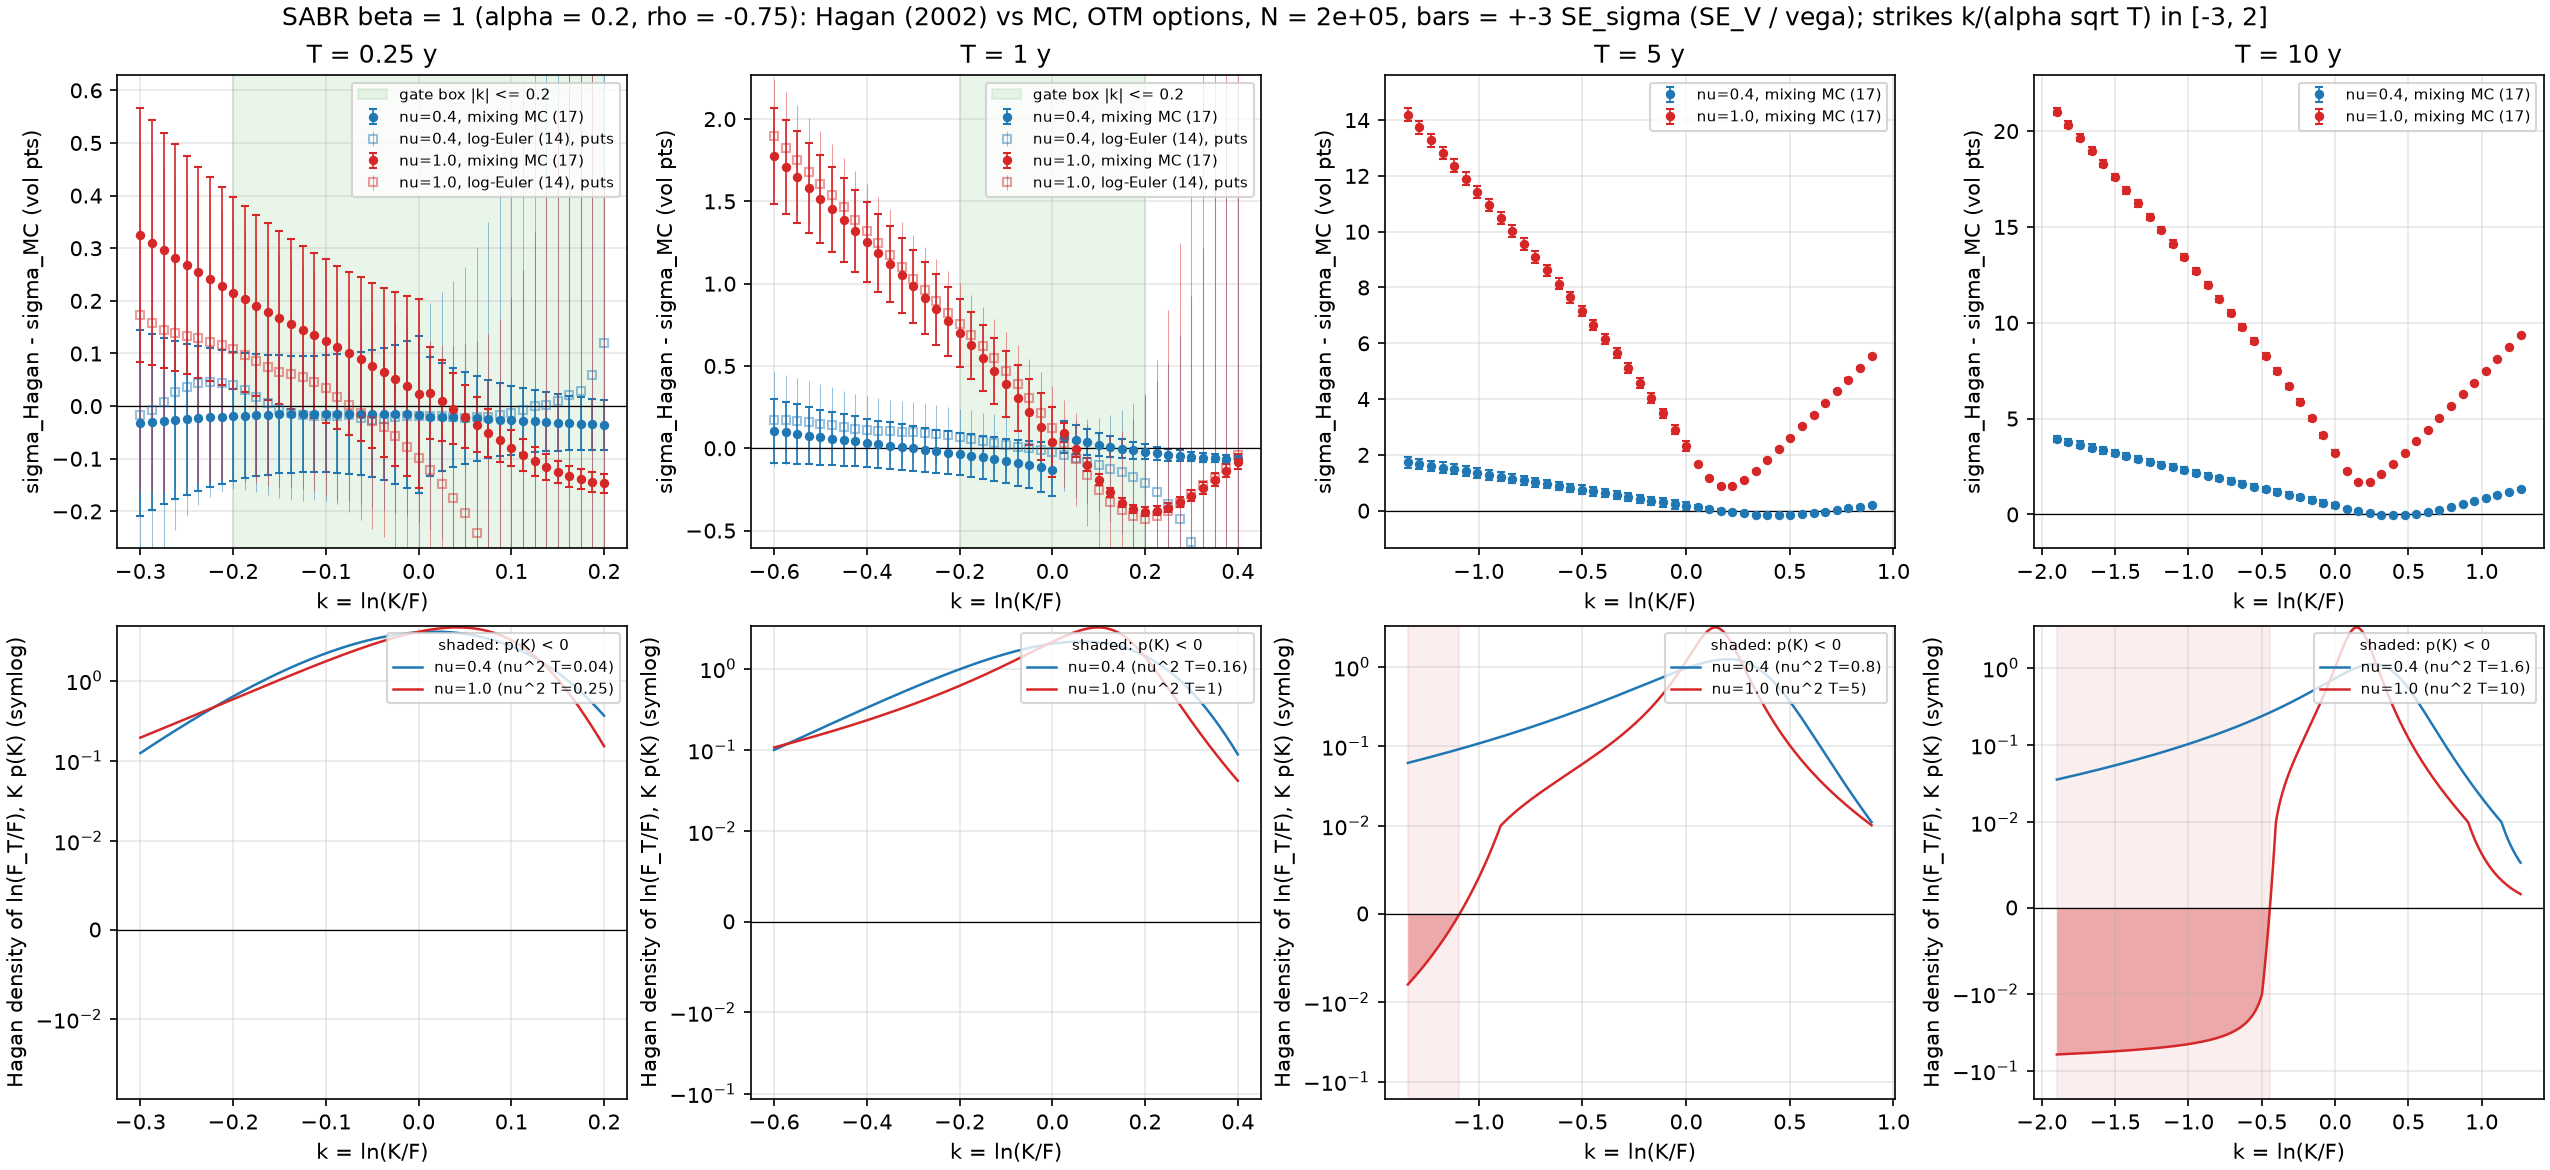
\includegraphics[width=\textwidth]{sabr_hagan_vs_mc.png}
\caption{SABR $\beta=1$ ($\alpha=0.2$, $\rho=-0.75$): Hagan against MC, OTM options, $N=2\times10^5$. Top row:
$\sigma_H-\sigma_{\text{MC}}$ in vol points with bars $\pm3\,\SE_\sigma$, for $\nu=0.4$ (blue) and $\nu=1$ (red), at
$T=0.25,1,5,10$; the green area is the gate box ($|k|\le0.2$). Bottom row: density implied by Hagan's formula
(second differences of Black), with negative-density regions shaded.}
\label{fig:sabr-hagan-mc}
\end{figure}

Figure~\ref{fig:sabr-hagan-mc} compares Hagan with the conditional estimator on strikes
$k/(\alpha\sqrt T)\in[-3,2]$. Table~\ref{tab:sabr-degr} reports, for each panel, the largest error among the points
resolved by the MC ($|z|>3$) and the minimum of the density $K\,p(K)$ implied by Hagan.

\begin{itemize}
\item The error grows with $\nu^2T$ and with $|k|$, and is largest at low strikes: Hagan is too high in the left wing.
\item The density becomes negative only at $\nu=1$ for $T=5$ and $T=10$, at low strikes.
\item Inside the gate box ($T\le1$, $|k|\le0.2$) at $\nu=0.4$ the error stays below the noise; at $\nu=1$ it does
not.
\end{itemize}

\begin{table}[t]
\centering
\small
\caption{Degradation of Hagan's formula ($\alpha=0.2$, $\rho=-0.75$): maximum error among the points resolved by
the MC, and minimum of the implied density.}
\label{tab:sabr-degr}
\begin{tabular*}{\textwidth}{@{\extracolsep{\fill}}rrrlrr@{}}
\toprule
$\nu$ & $T$ & $\nu^2T$ & max error (vol points) & at $k=$ & $\min K\,p(K)$\\
\midrule
0.4 & 0.25 & 0.04 & none resolved ($\max|z|=2.2$) & -- & $+0.12$\\
0.4 & 1 & 0.16 & 0.065 & $+0.40$ & $+0.088$\\
0.4 & 5 & 0.8 & 1.74 & $-1.34$ & $+0.011$\\
0.4 & 10 & 1.6 & 3.94 & $-1.90$ & $+0.0053$\\
1 & 0.25 & 0.25 & 0.33 & $-0.30$ & $+0.15$\\
1 & 1 & 1 & 1.78 & $-0.60$ & $+0.042$\\
1 & 5 & 5 & 14.2 & $-1.34$ & $-0.0080$\\
1 & 10 & 10 & 21.0 & $-1.90$ & $-0.061$\\
\bottomrule
\end{tabular*}
\end{table}

\subsection{\texorpdfstring{The validated domain: $\nu^2T\le0.16$}{The validated domain: ν²T ≤ 0.16}}
The gate holds for set G, that is, for $\nu^2T\le0.16$. An independent check, with a ``true'' model price computed
without the project code, shows that within the \emph{same} box ($T\le1$, $|k|\le0.2$) the gate fails as soon as
$\nu$ is realistic for the SPX:
\begin{itemize}
\item $\alpha=0.18$, $\rho=-0.7$, $\nu=1$, $T=0.5$ ($\nu^2T=0.5$): Hagan is $+0.40$ vol points above the model at
$k=-0.2$, that is, 5.4 SE;
\item $\alpha=0.2$, $\rho=-0.75$, $\nu=1$, $T=1$ ($\nu^2T=1$): $+0.82$ vol points at $k=-0.2$, that is, 10 SE.
\end{itemize}
This is the error of the Hagan expansion, not a code error.

\begin{attenzione}[title={Hagan as a parametrization, not as a model}]
In the SPX calibration (Chapter~\ref{cap:calibrazione}) \emph{every} expiry has $\nu^2T$ between 0.35 and 0.89,
outside the validated domain. The calibrated SABR smiles should therefore be read as \emph{parametrizations} of the
smile through Hagan's formula, not as the SABR dynamics. Pricing an exotic with a SABR MC on the same parameters
would give prices inconsistent with the vanillas used for calibration.
\end{attenzione}

\section{\texorpdfstring{Loss of martingality for $\rho>0$}{Loss of martingality for ρ>0}}
\label{sec:sabr-rho-pos}
For $\rho>0$ and $\beta=1$, $F$ is a \emph{strict} local martingale: $\E F_T<F$. Intuitively, with positive
correlation the volatility explodes precisely when the forward rises, and part of the mass ``escapes to infinity''.

The consequences are subtle.
\begin{itemize}
\item The log-Euler scheme \eqref{eq:sabr-euler} is an \emph{exact} martingale for every $\rho$. For $\rho>0$ its
calls (and those obtained via parity with $F$) target $P_{\text{model}}+\DF(F-K)$, not the model call.
\item The conditional estimator, on the other hand, prices the model call. The two methods of the same function
therefore have different expected values for calls with $\rho>0$; on puts they agree.
\item In the model, call and put implied volatilities at the same strike differ.
\item In practice the sample mean of $\hat F_T$ stays below $F$, because the missing mass lies on paths that are never
sampled: the error shows up as an unreliable SE rather than as a visible bias.
\end{itemize}
\begin{esempio}[title={Example: how large the effect is}]
$\alpha=0.3$, $\rho=+0.5$, $\nu=1$, $T=5$. Two independent methods give
\[
\frac{\E F_T}{F}-1=-0.1668\pm0.0003\qquad\text{and}\qquad{-0.1620}\pm0.0016 .
\]
At $\rho=-0.5$ the same computation gives $0.0000\pm0.0001$.
\end{esempio}

On the SPX $\rho<0$, so parity with $F$ holds. But the rule stands: parity with $F$ is the model's parity \emph{only}
for $\rho\le0$.

\section{Numerical pitfalls}
\begin{enumerate}
\item \textbf{$z/x(z)$ as $z\to0$}: $0/0$. Series for $|z|<10^{-3}$; and since \code{np.where} evaluates both
branches, $z$ is replaced by a dummy value in the direct branch.
\item \textbf{$\rho\to\pm1$}: cancellation in $x(z)$. Branch on sign and bound $|\rho|\le0.999$.
\item \textbf{Non-positive volatility} from $1+c_1T\le0$: \code{NaN} with a warning, never clip.
\item \textbf{Smile with arbitrage} in the wings and at long $T$: do not use the formula as a density source outside
its domain of validity.
\item \textbf{Hagan treated as the truth}: a gate at long $T$ or high $\nu$ fails because of the expansion, not the
code.
\item \textbf{Step bias}: the left-point integrated variance is low by about $\tfrac12\nu^2\Delta$; in the wings the
correlation term also matters. Steps per expiry and a size check.
\item \textbf{Trapezoidal rule only in the drift} of log-Euler: it breaks the martingale property.
\item \textbf{Heavy right tail}: calls with infinite variance for $\rho>-1/\sqrt2$. Simulate puts.
\item \textbf{Positivity}: Euler on $F$ or on $\alpha$ (instead of on their logarithms) can give negative values.
\item \textbf{Gate in volatility space}: inverting a noisy price can fail in the wings. Gate in price space.
\item \textbf{ATM inversion above the ceiling} for $\rho<0$: no root; \code{NaN}, never discard silently.
\end{enumerate}

\needspace{6\baselineskip}
\begin{riassunto}
\begin{itemize}
\item SABR: lognormal volatility correlated with the forward; $\beta=1$ chosen a priori (not identifiable, a choice of
dynamics).
\item Hagan: $\sigma_H=\alpha\,\big(z/x(z)\big)(1+c_1T)$; ``distance'' intuition with speed $D(\nu u)$. Evaluated
with a series, branching on sign, and \code{log1p}.
\item Three knobs: $\alpha$ level, $\rho\nu$ skew, $\nu^2/\alpha$ curvature. $\alpha$ from the ATM volatility by
solving a quadratic; for $\rho<0$ there is a ceiling $b^2/(4|a|)$.
\item MC: exact $\alpha$, log-Euler a martingale of order 1; conditional estimator of order 2. Gate on puts, in price
space, 250 steps at every expiry.
\item The formula holds for small $\nu^2T$: validated domain $\nu^2T\le0.16$. Beyond it, errors of tenths of a vol
point already at $T\le1$, and negative densities at large $\nu^2T$.
\item For $\rho>0$ the forward is not a martingale: parity with $F$ holds only for $\rho\le0$.
\end{itemize}
\end{riassunto}

\needspace{6\baselineskip}
\begin{domande}
\begin{enumerate}
\item Why is $\beta$ not calibrated? What changes if $\beta=1$ is chosen instead of $\beta=0.5$?
\item Explain intuitively why $\rho<0$ gives a negative skew.
\item Why is $2\sigma_{\mathrm{ATM}}/(b+\sqrt{b^2+4a\sigma_{\mathrm{ATM}}})$ used to invert the ATM volatility? When
does no solution exist?
\item Why is ``argument minus 1'' passed to \code{log1p} instead of computing the logarithm directly?
\item Why does the SABR MC compare puts, and why in price space?
\item The log-Euler scheme fails the 3 SE step-halving test: is there a bug? What proves it?
\item Under what conditions does Hagan's formula become unreliable, and how do you notice?
\item What happens to put--call parity with $F$ when $\rho>0$?
\end{enumerate}
\end{domande}


\part{Exotic options}
\chapter{Barrier options}
\label{cap:barriere}

A barrier option is the first ``path-dependent'' exotic one meets: the final payment is that of a vanilla, but it
counts only if the underlying has (or has not) touched a given level during the life of the contract. In this chapter
we derive the closed-form formulas with the reflection principle, build a Monte Carlo free of monitoring error,
explain the Broadie--Glasserman--Kou correction for barriers observed on discrete dates, and see what changes under
Heston. At the end we report the numbers measured in the project.

\section{What they are}
A barrier option is a European call or put that is \textbf{activated} (\emph{knock-in}) or \textbf{extinguished}
(\emph{knock-out}) if the underlying touches a level $H$ before expiry. There are eight combinations
(Table~\ref{tab:barriere-tipi}).
\begin{table}[htbp]
\centering
\small
\caption{The eight barrier options.}
\label{tab:barriere-tipi}
\begin{tabularx}{\textwidth}{>{\raggedright\arraybackslash}Xll}
\toprule
barrier & knock-out (``out'') & knock-in (``in'')\\
\midrule
\emph{down} ($S_0>H$, touched from above) & down-and-out call/put & down-and-in call/put\\
\emph{up} ($S_0<H$, touched from below) & up-and-out call/put & up-and-in call/put\\
\bottomrule
\end{tabularx}
\end{table}

We abbreviate with three letters: c/p (call/put), d/u (down/up), i/o (in/out). For example, cdo is the down-and-out
call.

Notation. $\theta=+1$ for the call and $-1$ for the put; $\eta=+1$ for a down barrier and $-1$ for an up barrier. Let
$\tau=\inf\{t\ge0:\eta(S_t-H)\le0\}$ be the first hitting time. Then
\begin{equation}
\text{knock-out: }(\theta(S_T-K))^+\,\ind\{\tau>T\},\qquad
\text{knock-in: }(\theta(S_T-K))^+\,\ind\{\tau\le T\}.
\end{equation}
Sometimes there is a \emph{rebate} $R$, a fixed refund: the out option pays it at the hit, the in option pays it at
expiry if the barrier was never touched. In the main tests $R=0$.

\begin{idea}[title={Key idea: in + out = vanilla}]
On every path the barrier either was touched or was not: exactly one of knock-in and knock-out pays. Hence
\begin{equation}\label{eq:in-out}
\text{knock-in}+\text{knock-out}=\text{vanilla}\qquad(R=0),
\end{equation}
in \emph{any} model. In a Monte Carlo, if in and out are computed on the same paths and with the same weights, the
identity must hold \emph{to rounding}, not within statistical error. If it fails by one standard error, in and out are
using different paths or weights. Beware of the test as well: computing ``in $:=$ vanilla $-$ out'' would turn the
check into a tautology. The two legs must be priced with separate calls.
\end{idea}

\paragraph{Barrier on spot or on forward.} Contracts (and published tables) define $H$ on the index level $S_t$, not
on the forward. Our kernels, however, work on the forward $F_t=F(t,T)$. The link is a \textbf{constant carry} $b$
(the ``cost of carry'' $b=r-q$), which is a kernel input with default 0:
\begin{equation}\label{eq:spot-da-forward}
S_t=F_t\,e^{-b(T-t)},\qquad S_0=F\,e^{-bT},\qquad S_T=F_T .
\end{equation}
With $b=0$ the barrier sits directly on the forward. The rate $r=-\ln\DF/T$ is derived from $\DF$ and is needed only
for the rebate paid at the hit. One could put a constant barrier on $F_t$, but for $b>0$ this is equivalent to a
barrier on the spot that rises over time, and the published tables are not reproduced.

\section{The reflection principle}
It is the key tool for the closed-form formulas.
\begin{proposizione}[Reflection, driftless Brownian motion]
Let $W$ be a Brownian motion started at 0 and $\ell<0$ a level. For every $y\ge\ell$:
\begin{equation}
\PP\Big(\min_{[0,T]}W\le\ell,\ W_T\ge y\Big)=\PP\big(W_T\le2\ell-y\big).
\end{equation}
\end{proposizione}
\emph{Idea.} Take every path that touches $\ell$ and \emph{reflect} it about $\ell$ after the first hit. Brownian
motion restarts from $\ell$ without memory and is symmetric, so the reflected path is equally likely. A path that has
touched $\ell$ and ends above $y$ corresponds to one that ends below $2\ell-y$. Conversely, every path that ends below
$2\ell-y\le\ell$ must have touched $\ell$. The correspondence is one-to-one.

\subsection{With drift: three steps}
Under Black with carry $b$, from \eqref{eq:spot-da-forward} the spot log-price $Y_t=\ln(S_t/S_0)$ is a Brownian
motion with drift:
\[
Y_t=\nu t+\sigma W_t,\qquad \nu=b-\tfrac12\sigma^2 .
\]
The barrier becomes the constant level $\ell=\ln(H/S_0)$. We define
\begin{equation}
\varrho=\frac H{S_0}=\frac HF\,e^{bT},\qquad \mu=\frac b{\sigma^2}-\frac12=\frac\nu{\sigma^2},\qquad F^*=\varrho^2F .
\end{equation}
For a down barrier ($\ell<0$) and any function $f$ we want the expectation
\[
\E\big[f(Y_T);\ \min_{[0,T]} Y\le\ell,\ Y_T>\ell\big].
\]

\noindent\textbf{Step 1 (remove the drift).} By Girsanov there is a measure $\tilde\Q$ under which $Y$ is a
driftless Brownian motion, with
\[
\frac{\dd\Q}{\dd\tilde\Q}=\exp\Big(\frac{\nu}{\sigma^2}Y_T-\frac{\nu^2T}{2\sigma^2}\Big).
\]
The expectation we want is therefore
\[
\tilde\E\Big[e^{\mu Y_T-\nu^2T/(2\sigma^2)}f(Y_T);\ \text{hit},\ Y_T>\ell\Big].
\]

\noindent\textbf{Step 2 (reflect).} Under $\tilde\Q$ reflection holds: the event $\{\text{hit},\,Y_T>\ell\}$ maps onto
$\{Y_T<\ell\}$ and $Y_T$ becomes $2\ell-Y_T$. The weight $e^{\mu Y_T}$ becomes
$e^{\mu(2\ell-Y_T)}=e^{2\mu\ell}e^{-\mu Y_T}$.

\noindent\textbf{Step 3 (go back).} Under $\tilde\Q$, $Y\mapsto-Y$ is also a symmetry. Applying it, the weight
$e^{-\mu Y_T}$ turns back into $e^{+\mu Y_T}$, that is, the density of $\Q$ again, and the event becomes
$\{2\ell+Y_T>\ell\}$. Result:
\begin{equation}\label{eq:immagine}
\E\big[f(Y_T);\ \text{hit }\ell,\ Y_T>\ell\big]=\varrho^{2\mu}\,\E\big[f(2\ell+Y_T);\ 2\ell+Y_T>\ell\big],
\end{equation}
because $e^{2\mu\ell}=e^{2\mu\ln\varrho}=\varrho^{2\mu}$.

\begin{idea}[title={The reflected world}]
The right-hand side contains $S_0e^{2\ell+Y_T}=\varrho^2S_T$, whose expectation is $\varrho^2F=F^*$. The ``reflected
world'' is therefore a Black world with \textbf{image forward} $F^*$, weighted by $\varrho^{2\mu}$. Every barrier
price is a combination of Black formulas in the true world and in the reflected world.
\end{idea}

\section{The Reiner--Rubinstein closed-form formulas in forward form}
We introduce the ``truncated'' Black formula with forward $X$ and cut-off level $L$:
\[
G(X,L;\kappa)=\theta\,\DF\big[X\,\Phi(\kappa\,d_1(X,L))-K\,\Phi(\kappa\,d_2(X,L))\big],\qquad
d_{1,2}(X,L)=\frac{\ln(X/L)}{\sigma\sqrt T}\pm\frac{\sigma\sqrt T}2 .
\]
The four building blocks are
\begin{align*}
A&=G(F,K;\theta)=\text{vanilla}, & B&=G(F,H;\theta),\\
C&=\varrho^{2\mu}\,G(F^*,K;\eta), & D&=\varrho^{2\mu}\,G(F^*,H;\eta).
\end{align*}
$B$ is the vanilla restricted to the scenarios with $S_T$ beyond the barrier; $C$ and $D$ are the reflected images of
$A$ and $B$. With the rebate two more terms are needed. Setting
\[
\lambda=\sqrt{\mu^2+2r/\sigma^2},\qquad z=\frac{\ln\varrho}{\sigma\sqrt T}+\lambda\sigma\sqrt T,
\]
we have
\begin{align*}
E&=R\,\DF\big[\Phi(\eta\,d_2(F,H))-\varrho^{2\mu}\,\Phi(\eta\,d_2(F^*,H))\big]=R\,\DF\,\Q(\tau>T),\\
\mathcal F&=R\big[\varrho^{\mu+\lambda}\,\Phi(\eta z)+\varrho^{\mu-\lambda}\,\Phi(\eta z-2\eta\lambda\sigma\sqrt T)\big]
=R\,\E\big[e^{-r\tau}\ind\{\tau\le T\}\big].
\end{align*}
$E$ is the rebate paid at expiry if the barrier is not touched, $\mathcal F$ the one paid at the hit (here
$\mathcal F$ is not a forward). The eight cases are in Table~\ref{tab:rr}.
\begin{table}[htbp]
\centering
\small
\caption{Reiner--Rubinstein prices of the eight barriers in terms of the building blocks $A$--$\mathcal F$.}
\label{tab:rr}
\begin{tabular*}{\textwidth}{@{\extracolsep{\fill}}lcclcc@{}}
\toprule
\multicolumn{3}{c}{knock-in} & \multicolumn{3}{c}{knock-out}\\
\cmidrule(r){1-3}\cmidrule(l){4-6}
type & $K\ge H$ & $K<H$ & type & $K\ge H$ & $K<H$\\
\midrule
cdi & $C+E$ & $A-B+D+E$ & cdo & $A-C+\mathcal F$ & $B-D+\mathcal F$\\
cui & $A+E$ & $B-C+D+E$ & cuo & $\mathcal F$ & $A-B+C-D+\mathcal F$\\
pdi & $B-C+D+E$ & $A+E$ & pdo & $A-B+C-D+\mathcal F$ & $\mathcal F$\\
pui & $A-B+D+E$ & $C+E$ & puo & $B-D+\mathcal F$ & $A-C+\mathcal F$\\
\bottomrule
\end{tabular*}
\end{table}

\subsection{How the table is assembled}
Each payoff is split on the event ``$S_T$ beyond the barrier'' (which forces a hit) and on its complement.
\begin{itemize}
\item \textbf{cdi with $K\ge H$.} It pays only if $S_T>K\ge H$. Starting above $H$, the path must have touched the
barrier and then come back up. By \eqref{eq:immagine} the price is the call in the reflected world:
$\varrho^{2\mu}\DF\,\E(\varrho^2S_T-K)^+=C$.
\item \textbf{cdi with $K<H$.} There are two pieces. If $S_T\le H$ the barrier was necessarily touched, and this
piece is worth $\DF\,\E[(S_T-K)^+;\,S_T\le H]=A-B$. If $S_T>H$ reflection is needed, which gives
$\varrho^{2\mu}\DF\,\E[(\varrho^2S_T-K);\,\varrho^2S_T>H]=D$.
\item \textbf{Puts and up barriers} are obtained with $\theta\to-1$ and $\eta\to-1$.
\item \textbf{Out options} are obtained as vanilla minus in, plus the rebate legs.
\end{itemize}
Adding an ``in'' row and the corresponding ``out'' row gives back $A+E+\mathcal F$: with $R=0$ this is
\eqref{eq:in-out}.

\paragraph{Barrier already touched.} The table requires $\eta\ln\varrho<0$. If the barrier has already been crossed
($\eta(S_0-H)\le0$), with continuous monitoring the out option is worth the rebate and the in option is worth the
vanilla. The two columns coincide at $K=H$ (because $A=B$ and $C=D$), and the table tends continuously to this case as
$\varrho\to1$.

\subsection{The zero-carry case: static hedging}
With $b=0$ we have $\mu=-\frac12$, hence $\varrho^{2\mu}=F/H$ and $F^*=H^2/F$. Using the homogeneity and the
put--call symmetry of Chapter~\ref{cap:black}:
\begin{equation}
\text{cdi}=\frac FH\,\mathrm{Call}\Big(\frac{H^2}{F},K\Big)=\frac KH\,\mathrm{Put}\Big(F,\frac{H^2}{K}\Big)\qquad(K\ge H).
\end{equation}
\begin{idea}
The down-and-in call is worth $K/H$ puts with strike $H^2/K$. This is a \textbf{static hedge}. I buy those puts. If
the barrier is touched, at that instant (by put--call symmetry) the puts are worth exactly as much as the call that is
activated, and I swap them at zero cost. If it is not touched, the puts expire worthless, like the down-and-in. The
hedge breaks down with carry (the factor $\varrho^{2\mu}$) and with a skew, because put--call symmetry requires a smile
that is symmetric in log-moneyness.
\end{idea}

\subsection{A model-free result}
With $b=0$ and $K=H$ a down-and-out call is worth exactly
\begin{equation}\label{eq:cdo-model-free}
\text{cdo}(K=H)=\DF\,(F-H)\qquad\text{for \emph{any} continuous martingale }F\text{ (Heston included).}
\end{equation}
\emph{Proof.} $F$ is a continuous martingale and $\tau$ a stopping time, so by the optional stopping theorem
$\E F_{T\wedge\tau}=F$. If the barrier is touched, by continuity $F_\tau=H$. Hence
$\E[(F_T-H)\ind\{\tau>T\}]=F-H$, and on $\{\tau>T\}$ the payoff of the call with $K=H$ is exactly $F_T-H>0$. Only
continuity and the martingale property have been used. It is a valuable test for Monte Carlo under Heston, where no
other closed-form formulas exist.

\section[Continuously monitored Monte Carlo: the Brownian bridge]{Continuously monitored Monte Carlo:\\
  the Brownian bridge}
\subsection{The problem with naive Monte Carlo}
If we simulate on a grid and check the barrier only at the nodes, we miss the paths that cross the barrier
\emph{between} two nodes and come back. In fact we are pricing a contract with discrete monitoring on $m$ dates, not a
continuous one. Knock-outs come out too expensive. The error decreases only like $\sqrt{\Delta t}$ (as
\eqref{eq:bias-monitoraggio} will show): halving the step removes only about 29\% of it.

\begin{esempio}
Down-and-out call with the inputs of table 2.1 of Broadie--Glasserman--Kou: $K=100$, $H=95$, $\sigma=0.30$, $T=0.2$,
$b=0.1$. The continuous closed-form formula gives 4.3975. Naive Monte Carlo with $m=4$ dates gives 5.785; with
$m=512$ it still gives 4.582, that is, 0.185 too high. Monte Carlo with the Brownian bridge gives 4.404 and 4.403 at
the same $m$.
\end{esempio}

\subsection{The crossing probability, step by step}
Given the values at two consecutive nodes, the probability that the path in between has touched the barrier is known
exactly. Consider a step of length $\Delta$ and a down barrier. Let $a=Y_{t_i}$ and $c=Y_{t_{i+1}}$ be the log-prices
at the two endpoints, both above $\ell$, and $A=a-\ell>0$, $C=c-\ell>0$ the log-distances from the barrier.

\noindent\textbf{Step 1.} Apply \eqref{eq:immagine} on the interval $[t_i,t_{i+1}]$, starting from $a$ (the level,
measured from the starting point, is $\ell-a$). The density of ``arriving at $c$ having touched $\ell$'' is
$e^{2\nu(\ell-a)/\sigma^2}$ times the Gaussian density of a reflected increment, equal to $(c-a)-2(\ell-a)=c+a-2\ell$.

\noindent\textbf{Step 2.} The conditional probability of having touched is the ratio of this density to the free
density of arriving at $c$, that is, of an increment $c-a$. The increments are Gaussian with mean $\nu\Delta$ and
variance $\sigma^2\Delta$, hence
\[
p=\exp\!\Big(\frac{2\nu(\ell-a)}{\sigma^2}-\frac{(c+a-2\ell-\nu\Delta)^2-(c-a-\nu\Delta)^2}{2\sigma^2\Delta}\Big).
\]

\noindent\textbf{Step 3.} Expand the squares with $a^2-b^2=(a-b)(a+b)$. The difference of the two increments is $2A$,
their sum is $2C-2\nu\Delta$: the numerator is $2A(2C-2\nu\Delta)=4AC-4\nu\Delta A$. The term $-4\nu\Delta A$,
divided by $2\sigma^2\Delta$, exactly cancels the first summand $2\nu(\ell-a)/\sigma^2=-2\nu A/\sigma^2$, leaving
\begin{equation}\label{eq:bb}
p_i=\exp\!\Big(-\frac{2\,A\,C}{\sigma^2\Delta}\Big).
\end{equation}
\begin{perche}[title={Why the drift disappears}]
Conditional on its endpoints, a Brownian motion with drift is a \emph{Brownian bridge}: the drift only shifts the end
point, which is already fixed. This is why \eqref{eq:bb} holds for any carry. A barrier that is linear in time (such
as our spot barrier seen in forward coordinates) also amounts to changing the drift, so the formula stays exact.
\end{perche}
In general form, with $y_i=\ln(S_{t_i}/H)$ the signed log-distance:
\[
p_i=\exp\!\Big(-\frac{2\,(\eta y_i)^+\,(\eta y_{i+1})^+}{\sigma_i^2\,\Delta}\Big).
\]
The positive parts automatically give $p_i=1$ (dead path) when an endpoint is on or beyond the barrier.

\subsection{The survival weight}
Instead of drawing a uniform to decide whether the path survived, the probability is used directly:
\begin{equation}\label{eq:peso-bb}
\begin{gathered}
w=\prod_i(1-p_i),\\
\text{out sample}=g\,w,\qquad\text{in sample}=g\,(1-w),\qquad\text{vanilla}=g,
\end{gathered}
\end{equation}
with $g=(\theta(S_T-K))^+$. Since $gw+g(1-w)=g$ on every path, \eqref{eq:in-out} holds to rounding.
\begin{perche}[title={Why the weight and not the uniform}]
Let $I=\prod_i\ind\{U_i>p_i\}$ be the indicator drawn with the uniforms. Then $\E[I\mid\text{path}]=w$ and
$\Var[I\mid\text{path}]=w(1-w)$, hence
\[
\Var(gI)=\Var(gw)+\E\big[g^2w(1-w)\big].
\]
The expectation is the same, but the variance with the uniform is larger. Replacing a random variable with its
conditional expectation always reduces the variance (Rao--Blackwell). In addition, $w$ is smooth in the parameters,
which makes Greeks computed with common random numbers stable. Under Black the estimator is \emph{exact} for any
number of steps, even a single one.
\end{perche}

\begin{attenzione}[title={Numerical details}]
\begin{itemize}
\item If $\sigma_i^2\Delta=0$ (under Heston $v_i^+=0$ can happen) and an endpoint lies exactly on the barrier, the
formula gives $0/0$. The code sets $p_i=0$ or $1$ depending on whether the product $AC$ is positive or zero.
\item For distant paths the exponential underflows to 0: that is the right value.
\item In and out must use the same set of paths, the same $w$ and the same ``alive if $\eta y>0$'' rule. Different
seeds, a re-drawn uniform for the in leg, or different tie-breaking rules break the identity by one standard error.
\item Spot and forward must be consistent between formula and Monte Carlo. A different $b$ in the two gives an error
proportional to $bT$ that no refinement removes. In the code a single expression computes the $y_i$.
\end{itemize}
\end{attenzione}

\section{Discretely observed barriers: the BGK correction}
Many contracts check the barrier only on fixed dates, for example at each close. Broadie, Glasserman and Kou showed
that the price with $m$ dates equals the continuous price with the barrier \emph{shifted away from the spot}:
\begin{equation}\label{eq:bgk}
\begin{gathered}
V_m(H)=V\big(H\,e^{-\eta\,\beta\,\sigma\sqrt{\Delta t}}\big)+o(m^{-1/2}),\\
\beta=-\frac{\zeta(1/2)}{\sqrt{2\pi}}=0.5825971579\ldots,\qquad\Delta t=\frac Tm .
\end{gathered}
\end{equation}
A down barrier moves down, an up barrier moves up. $V$ is the Reiner--Rubinstein formula at the shifted barrier. The
result is proved under Black for all eight types; under Heston it has no justification.

\subsection{\texorpdfstring{Where $0.5826$ comes from}{Where 0.5826 comes from}}
\noindent\textbf{Step 1 (the overshoot).} A random walk observed only on the dates $t_j$, when it first exceeds a
level, has already ``overshot'' it by an amount $R_m>0$. The continuous path, by contrast, stops exactly on the
barrier.

\noindent\textbf{Step 2 (reflect at the right point).} The discrete price is obtained by reflecting at the point
where the path is actually observed beyond the barrier, that is, at a distance $R_m$ beyond $H$. On average, for a
distant level, the overshoot measured in standard deviations of one step tends to a constant $\beta$ (Siegmund's
constant for Gaussian steps). Reflecting at $H$ shifted by $\beta\sigma\sqrt{\Delta t}$ is equivalent to pricing the
discrete contract.

\noindent\textbf{Step 3 (the value of $\beta$, sketch).} Spitzer's formula expresses the ``ladder'' heights of a
random walk through series of the type $\sum_n n^{-1}\E[S_n^-]$, where $S_n$ is the sum of $n$ steps. For standard
Gaussian steps $\E[S_n^-]=\sqrt n/\sqrt{2\pi}$, so the series is $(2\pi)^{-1/2}\sum_n n^{-1/2}$, which diverges. The
divergent part is the same as in the continuous case and cancels in the comparison; what remains is the finite part
\[
\lim_{N\to\infty}\Big(\sum_{n\le N}n^{-1/2}-2\sqrt N\Big)=\zeta(1/2)\approx-1.4604 .
\]
Hence $\beta=-\zeta(1/2)/\sqrt{2\pi}$.

\subsection{Monitoring bias and the pre-asymptotic slope}
Expanding \eqref{eq:bgk} to first order in $\Delta t$:
\begin{equation}\label{eq:bias-monitoraggio}
V_m(H)-V(H)\approx-\eta\,\beta\,\sigma\sqrt{\Delta t}\;H\,\partial_HV(H)=O(m^{-1/2}).
\end{equation}
One therefore expects slope $1/2$ on a log-log plot of the naive Monte Carlo error against $\Delta t$.
\begin{attenzione}[title={Slope 0.42, not 0.5: not an error}]
On the down-and-out of the example ($H=95$), for $m$ from 4 to 512 the estimated slope of the naive Monte Carlo bias
is \textbf{0.422}. The deterministic BGK prediction, ${V(He^{-\beta\sigma\sqrt{\Delta t}})-V(H)}$, on the same $m$
gives \textbf{0.426}. Its local slope rises from 0.32 (between $m=4$ and $m=8$) and reaches 0.50 only for
$m\approx10^6$. An independent check with exact discrete prices (backward quadrature) gives 0.4295.

\smallskip
The reason: $\frac12$ is the \emph{asymptotic} order. At practical values of $m$ the barrier shift is not small
relative to the curvature of $V$ at $H$, and the higher-order terms of \eqref{eq:bias-monitoraggio} matter. The Monte
Carlo matches the deterministic prediction: it must not be ``corrected'' towards 0.5.
\end{attenzione}

\begin{figure}[htbp]
\centering
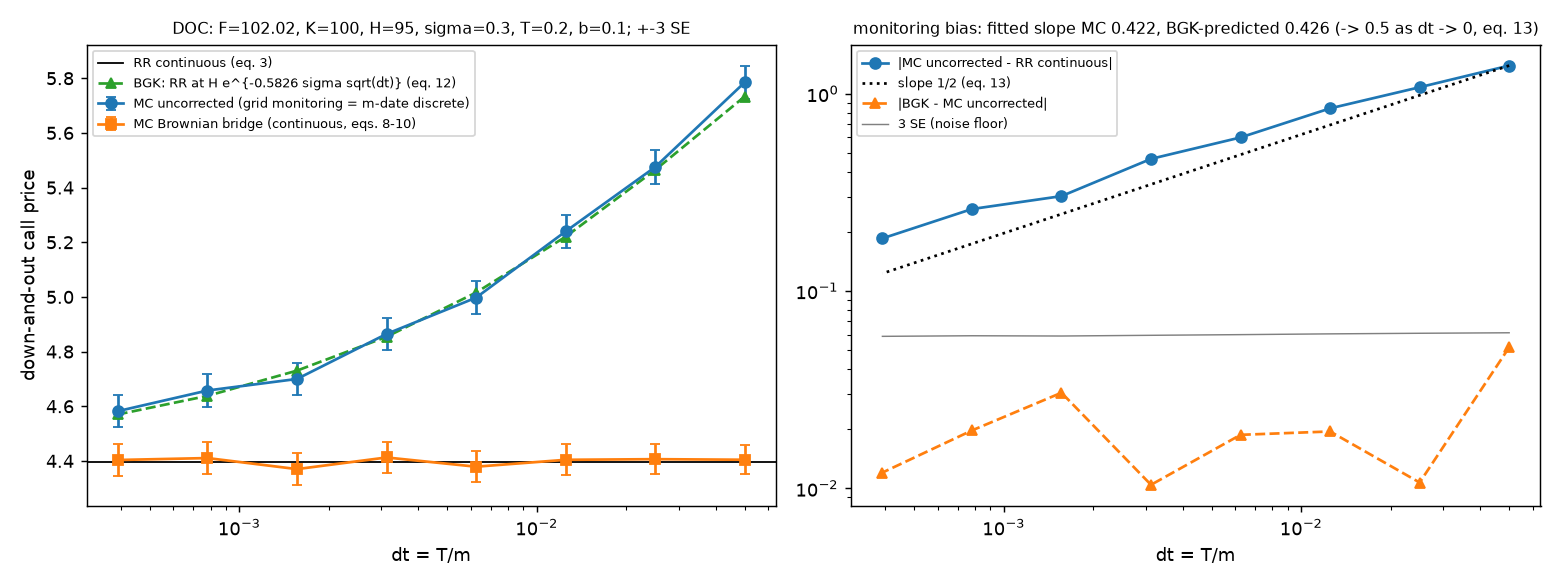
\includegraphics[width=\textwidth]{barrier_mc_vs_rr.png}
\caption{Down-and-out call ($F=102.02$, $K=100$, $H=95$, $\sigma=0.3$, $T=0.2$, $b=0.1$), bars at $\pm3$ SE,
$2\times10^5$ paths per point. Left: naive Monte Carlo (which prices the $m$-date contract), continuous formula at the
BGK-shifted barrier, Brownian-bridge Monte Carlo and continuous formula. Right: naive Monte Carlo bias on a log-log
scale, with estimated slope 0.422 against the line of slope $\frac12$.}
\label{fig:barrier-mc-rr}
\end{figure}

Figure~\ref{fig:barrier-mc-rr} sums it all up. On the left, naive Monte Carlo (blue) slowly falls towards the
continuous price and agrees, within error, with the BGK formula (green): it is pricing the discrete contract. The
Brownian bridge (orange) sits on the continuous formula for every $\Delta t$. On the right, the difference between BGK
and naive Monte Carlo stays below the 3 SE threshold.

\subsection{Where BGK works and where it does not}
Table~\ref{tab:bgk} compares the correction with the published discrete values.

\begin{table}[htb]
\centering
\small
\caption{BGK correction against the discrete price ($K=100$, $\sigma=0.30$, $T=0.2$, $b=0.1$).}
\label{tab:bgk}
\begin{tabular*}{\textwidth}{@{\extracolsep{\fill}}lrrrrrl@{}}
\toprule
case & $m$ & $H$ & true & BGK & relative error & note\\
\midrule
DOC, $S_0=100$ & 50 & 85 & 6.322 & 6.3223 & $+0.11\%$ & \\
DOC & 50 & 95 & 4.907 & 4.9071 & $-0.03\%$ & \\
DOC & 50 & 98 & 3.126 & 3.1210 & $-0.63\%$ & \\
DOC & 50 & 99 & 2.337 & 2.2713 & $-3.10\%$ & close to the barrier\\
DOC & 5 & 99 & 4.489 & 4.0495 & $-9.23\%$ & \\
UOC, $S_0=110$ & 50 & 115 & 0.807 & 0.8188 & $+1.56\%$ & reverse\\
\bottomrule
\end{tabular*}
\end{table}

``True'' is the discrete value published by BGK; the relative error is measured against the project's discrete Monte
Carlo (exact steps at the dates). Far from the barrier the error is a few hundredths of a percentage point. Within
about one step standard deviation of the barrier the correction degrades; there the discrete Monte Carlo is used. By
construction, with the dates on the grid nodes, path by path continuous knock-out $\le$ discrete knock-out.

\section{Barriers under Heston: the bridge on the variance}
Under Heston the same formula \eqref{eq:bb} is used with the variance at the start of the step, $\sigma_i^2=v_i^+$.
\begin{perche}[title={Why the bridge is not exact here}]
Given the variance path, $\ln S$ is Gaussian with a variance that changes over time and a drift that depends on $v$.
Freezing $v$ at its value at the start of the step is the ``local volatility'' rule: it is exact only as
$\Delta\to0$. Moreover, in a step with $v_i^+=0$ the path cannot cross. We therefore expect some exits to be missed
and knock-outs to come out slightly too expensive: a positive bias of order $\Delta$.
\end{perche}
\begin{progetto}[title={In the qpricer project: the measured residual bias}]
Oracle: \eqref{eq:cdo-model-free}, cdo$(K=H=90)=10\,\DF$, on a Heston parameter set that violates Feller (the FO set
of Chapter~\ref{cap:mc}), QE-M scheme. An independent check averaged 25 seeds for each step:
\begin{center}
\small
\begin{tabular}{lcccc}
\toprule
$\Delta$ & 1/32 & 1/64 & 1/128 & 1/256\\
\midrule
bias of cdo $-10\,\DF$ & $+0.095$ & $+0.055$ & $+0.020\pm0.005$ & $+0.012\pm0.005$\\
\bottomrule
\end{tabular}
\end{center}
The bias is of order $\Delta$ and positive, as predicted. The 3 SE test with $2\times10^5$ paths passes at
$\Delta=1/128$ ($z=+0.75$) because $0.020$ is below the standard error of the test (0.024), \emph{not} because the
bias is zero. At $\Delta=1/64$ about 16\% of the seeds would fail. For tighter accuracy $\Delta\le1/256$ is used.
BGK is not used under Heston: discrete contracts are priced with the discrete Monte Carlo.

\smallskip
Second test: with $\xi=10^{-4}$, $\rho=0$ Heston becomes Black with $\sigma=\sqrt\theta$. Maximum $|z|=2.97$ on the
declared seed. It is an unlucky seed (about one in 75): on the same set of paths the vanilla is also off by $-3.15$
and $+3.13$ SE, and the barrier $z$ tracks the vanilla $z$ with correlation 0.905. Over 300 independent seeds the mean
$z$ per cell lies between $-0.031$ and $+0.011$: no bias. The seed was not changed.
\end{progetto}

\section{The case of Haug's table}
Haug's (1998) table is the classic reference for barriers: $S_0=100$, $r=8\%$, $b=4\%$, $T=0.5$, rebate $R=3$,
continuous monitoring. In forward form: $F=100e^{0.02}=102.0201340$, $\DF=e^{-0.04}$, carry $b=0.04$. There are 72
cells (12 type$\times$barrier combinations, three strikes, $\sigma\in\{0.25,0.30\}$) rounded to four decimals, so the
natural tolerance is $5\times10^{-5}$. For example, cdo with $H=95$, $K=100$, $\sigma=0.25$ is worth 6.7924.

\begin{esempio}[title={Example: six published values that do not add up}]
66 cells out of 72 meet $5\times10^{-5}$: maximum $4.96\times10^{-5}$ at $\sigma=0.25$ and $4.59\times10^{-5}$ at
$\sigma=0.30$. Six cells at $\sigma=0.30$, however, are off by $5.2$--$6.25\times10^{-5}$: cuo($H=105$, $K=90$),
puo($H=105$, $K=90,100,110$) and pdi($H=95$, $K=100,110$). For example, puo with $K=90$ is worth $4.22923747$, but the
table prints 4.2293.
\end{esempio}

\paragraph{Suspect the math first.} The rule is to suspect the math first, then the code, and the reference last.
Three mutually independent methods agree on those six cells:
\begin{itemize}
\item direct quadrature of the ``killed'' density and of the first-passage density, without using the algebra of the
building blocks $A$--$\mathcal F$: it agrees with Reiner--Rubinstein to within $3.2\times10^{-14}$;
\item an independent transcription of Reiner--Rubinstein in Haug's spot form;
\item a partial differential equation solved with Crank--Nicolson, which does not use reflection: it agrees with the
spot form to within $5.5\times10^{-10}$.
\end{itemize}
The discrepancies are one unit in the fourth decimal place, and no small perturbation of $(\sigma,T,r,b)$ explains the
column better. Conclusion: those six printed values are not correctly rounded.

\paragraph{How it was handled, without loosening the tolerance.} A first attempt had moved the entire $\sigma=0.30$
column to $10^{-4}$. That was wrong: it also loosened 30 cells that pass at $5\times10^{-5}$. An independent check
flagged it and that version was withdrawn. The final treatment is per cell:
\begin{itemize}
\item the 66 correctly rounded cells stay at $5\times10^{-5}$ against the published value;
\item the six wrong cells are flagged as such in a reference file built with the two independent methods
(\path{tests/golden/barrier_haug.json}) and are tested against that value at $10^{-10}$ (measured
$3.46\times10^{-14}$);
\item all 72 cells are also tested against the reference file at $10^{-10}$ (measured $4.80\times10^{-14}$).
\end{itemize}
The criterion did not change: the reference changed for six cells, and the test became tighter, not looser.

\section{Risks and pitfalls}
\begin{itemize}
\item \textbf{Greeks near the barrier.} A knock-out with a non-zero payoff at the barrier (``reverse'', for example
cuo with $K<H$ or pdo with $K>H$) jumps by $|H-K|$ at the hit. Near expiry delta and gamma explode and the hedge is
not smooth: hedging a discontinuity would require unbounded trades. Vega near the barrier is negative (more volatility
means a higher probability of being knocked out). The price depends on the volatility \emph{at the barrier} and on the
forward skew, not on the ATM volatility: this is why Black and Heston give different prices.
\item \textbf{Finite differences that cross the barrier.} A bump of $S$ that goes past $H$ jumps to the ``barrier
already touched'' branch. The bump must be less than half the distance to $H$; in Monte Carlo common random numbers
are used with the smooth weight $w$, never the discrete indicator.
\item \textbf{Computing $\varrho^{2\mu}\Phi(\cdot)$ with small $\sigma$.} $\mu=b/\sigma^2-\frac12$ is large and the
product can give $\infty\cdot0$. The code works in logarithms:
$\exp\big(2\mu\ln\varrho+\log\Phi(\cdot)\big)$, with \code{log\_ndtr}.
\item \textbf{Negative rates with a rebate.} If $\DF>1$, $\lambda^2=\mu^2+2r/\sigma^2$ can be negative and
$\mathcal F$ does not exist: with $R>0$ an error is raised.
\item \textbf{Many 3 SE tests.} With eight types, several strikes and several barriers, about 0.27\% of the
comparisons fail even with correct code. The seed is fixed, every failure is diagnosed, and the seed is never changed
to make a test pass.
\end{itemize}

\needspace{22\baselineskip}
\begin{progetto}[title={In the qpricer project: code and results}]
The closed-form formula is \code{barrier\_price} in \path{src/qpricer/engines/analytic.py}; the Monte Carlo is
\code{barrier\_mc} in \path{src/qpricer/engines/exotic_mc.py}, with the weight \eqref{eq:peso-bb} computed by
\code{bridge\_survival}. Tests in \path{tests/test_barrier.py}.
\begin{center}
\small
\begin{tabularx}{\textwidth}{>{\raggedright\arraybackslash}Xll}
\toprule
check & measured & threshold\\
\midrule
in + out = vanilla, same paths (8 types, Black and Heston, continuous and discrete) & $3.55\times10^{-15}$ &
$<10^{-12}$\\
Brownian bridge vs Reiner--Rubinstein, 56 cells, $b\in\{0,0.04\}$, $M\in\{1,50\}$ & $\max|z|=1.99$ & 3 SE\\
Heston $\xi=10^{-4}$ vs Reiner--Rubinstein at $\sqrt\theta$ & $\max|z|=2.97$ & 3 SE\\
Heston, cdo$(K=H)=10\,\DF$ at $\Delta=1/128$ & $z=+0.75$ & 3 SE\\
continuous formula and BGK vs BGK tables & $4.97\times10^{-4}$ & $5\times10^{-4}$\\
discrete Monte Carlo vs BGK ``true'' values (13 cells) & $\max|d|/(3\mathrm{SE}+10^{-3})=0.54$ & $\le1$\\
Haug, 66 correctly rounded cells & $4.96\times10^{-5}$ & $5\times10^{-5}$\\
Haug, 6 wrong cells vs independent reference & $3.46\times10^{-14}$ & $10^{-10}$\\
\bottomrule
\end{tabularx}
\end{center}
The cells that must be exactly zero (cuo with $K\ge H$, pdo with $K\le H$) are exactly zero in Monte Carlo as well.
Over 2800 $z$ values obtained with fresh seeds, an independent check found mean $+0.026$, standard deviation 0.998 and
0.36\% beyond 3 (expected 0.27\%).
\end{progetto}

\needspace{6\baselineskip}
\begin{riassunto}
\begin{itemize}
\item Eight types; in + out = vanilla in every model. In Monte Carlo, on the same paths, it holds to rounding.
\item Reflection + Girsanov $\Rightarrow$ reflected world with forward $F^*=\varrho^2F$ and weight $\varrho^{2\mu}$;
the Reiner--Rubinstein formulas are combinations of Black formulas.
\item Zero carry: static hedge with $K/H$ puts of strike $H^2/K$. $\text{cdo}(K=H)=\DF(F-H)$ for every continuous
martingale.
\item Continuous Monte Carlo: weight $\prod(1-p_i)$ with $p_i=e^{-2AC/(\sigma^2\Delta)}$, exact under Black for any
step.
\item Discrete monitoring: barrier shifted by $0.5826\,\sigma\sqrt{\Delta t}$ (BGK). Measured bias slope 0.42: it is
pre-asymptotic, not an error.
\item Under Heston the bridge with $v_i^+$ has a bias of order $\Delta$ (+0.020 at $\Delta=1/128$).
\item Six of Haug's values are wrongly rounded: handled per cell against an independent reference, without loosening.
\end{itemize}
\end{riassunto}

\needspace{9\baselineskip}
\begin{domande}
\begin{enumerate}
\item Why does in + out = vanilla hold in every model? Why must it hold to $10^{-12}$ in Monte Carlo and not within
3 SE?
\item Derive \eqref{eq:immagine} in three steps (Girsanov, reflection, symmetry).
\item Derive the crossing probability \eqref{eq:bb} and show that the drift cancels.
\item Why does the weight $w$ have lower variance than the drawn uniform?
\item Why is a knock-out with a daily-observed barrier worth more than one with a continuous barrier? Where does
$0.5826$ come from?
\item The measured slope is 0.42 instead of 0.5: what do you check before calling it an error?
\item What is special about the down-and-out call with $K=H$ at zero carry? Why is it useful under Heston?
\item Six published values fail the tolerance. How do you proceed?
\end{enumerate}
\end{domande}

\chapter[Asian options and control variates]{Asian options\\ and control variates}
\label{cap:asiatiche}

The arithmetic Asian option is the textbook case in which Monte Carlo is unavoidable but can be made very efficient.
Its geometric ``twin'' has a closed-form formula, and that formula is used twice: as an oracle for the Monte Carlo and
as a control variate. In this chapter we derive the formula, the optimal control coefficient and the variance-reduction
factor, then we see why the control is valid only under Black and which error surfaced under Heston.

\section{The product}
An arithmetic Asian option pays on the \emph{average} of the prices observed on $n$ fixed dates (\emph{fixings})
$t_1<\dots<t_n$ in $[0,T]$:
\begin{equation}
A=\frac1n\sum_{i=1}^nS_{t_i},\qquad\text{payoff }(\theta(A-K))^+\ \text{paid at }T .
\end{equation}
Why they exist: they are cheaper than vanillas (the average fluctuates less than a single price) and they are robust
to a single anomalous or manipulated settlement price. The geometric twin uses $G=\big(\prod_iS_{t_i}\big)^{1/n}$. On
the same paths we denote the discounted payoffs by
\[
Y=\DF\,(\theta(A-K))^+,\qquad X=\DF\,(\theta(G-K))^+.
\]

\section{The fixing forwards}
With deterministic rates and carry, the expected value of each fixing is the forward for that date:
\begin{equation}\label{eq:forward-fixing}
\E[S_{t_i}]=F(0,t_i)=:F_i,\qquad\E[A]=\bar A_F=\frac1n\sum_iF_i,\qquad V_A=\DF\cdot\E[(\theta(A-K))^+].
\end{equation}
\emph{Why.} $S_t=F(t,T)\,F(0,t)/F(0,T)$ and $F(\cdot,T)$ is a martingale, hence $\E S_t=F(0,t)$. With a constant
carry $b$, $F_i=F\,e^{-b(T-t_i)}$ and $\partial F_i/\partial b=-(T-t_i)F_i$: the price is sensitive to the timing of
dividends.
\begin{attenzione}
The price depends on the \emph{whole} curve $F_1,\dots,F_n$, not only on $F(0,T)$. The Monte Carlo and the closed
form use the same curve, so a Monte Carlo versus formula comparison \emph{cannot} reveal a wrong curve (for example
$F(0,T)$ for every fixing, or interpolating $F$ instead of $\ln F$). The curve builder must be tested separately. In
the project, for the SPX, $\ln F$ (and $\ln\DF$) is interpolated linearly between the expiries obtained from parity;
a fixing at time zero enters with $F(0,0)=S_0$, supplied by the caller.
\end{attenzione}

\section{The closed form for the geometric (discrete Kemna--Vorst)}
Under Black every $S_{t_i}$ is lognormal, but a \textbf{sum} of lognormals is not lognormal: there is no closed form
for $A$. A \textbf{product} of lognormals, on the other hand, is lognormal, because the logarithm turns the product
into a sum of Gaussians. We derive the formula for arbitrary dates.

\noindent\textbf{Step 1 (law of the fixings).} Let $V(t)=\int_0^t\sigma^2(s)\dd s$ be the total variance up to $t$
(with constant $\sigma$, $V(t)=\sigma^2t$). As in Chapter~\ref{cap:strumenti},
\[
\ln S_{t_i}=\ln F_i-\tfrac12V(t_i)+M_{t_i},\qquad M_t=\int_0^t\sigma\dd W,\qquad\Cov(M_s,M_t)=V(\min(s,t)).
\]
The covariance of a stochastic integral is the variance accumulated up to the smaller time.

\noindent\textbf{Step 2 (mean of $\ln G$).} $\ln G=\frac1n\sum_i\ln S_{t_i}$ is a linear combination of Gaussians,
hence Gaussian. Its mean is
\begin{equation}\label{eq:mu-G}
\mu_G=\ln\bar G_F-\tfrac12\bar V,\qquad\bar G_F=\Big(\prod_iF_i\Big)^{1/n},\qquad\bar V=\frac1n\sum_iV(t_i).
\end{equation}

\noindent\textbf{Step 3 (variance of $\ln G$).} It is the variance of $\frac1n\sum_iM_{t_i}$:
\begin{equation}\label{eq:sigma-G}
\sigma_G^2=\frac1{n^2}\sum_{i,j}V(\min(t_i,t_j))=\frac1{n^2}\sum_{i=1}^n(2n-2i+1)\,V(t_i)=\sum_{k=1}^nw_k^2\,\Delta V_k ,
\end{equation}
with $\Delta V_k=V(t_k)-V(t_{k-1})$, $t_0=0$ and $w_k=(n-k+1)/n$. The second form counts the pairs $(i,j)$ whose
minimum equals $i$: there are $2(n-i)+1$ of them. The third (Abel form) writes $\sum_iM_{t_i}=\sum_k(n-k+1)\Delta M_k$
with independent increments: each increment is shared by all later fixings, and therefore carries weight
$\big((n-k+1)/n\big)^2$.

\noindent\textbf{Step 4 (forward of $G$).} For a lognormal $\E G=e^{\mu_G+\sigma_G^2/2}$:
\begin{equation}\label{eq:FG}
F_G=\bar G_F\exp\!\big(-\tfrac12(\bar V-\sigma_G^2)\big).
\end{equation}

\noindent\textbf{Step 5 (Black formula).} The derivation of Chapter~\ref{cap:black} uses only the fact that
$\ln F_T\sim\N(\ln F-s^2/2,\,s^2)$. Here $\ln G\sim\N(\ln F_G-\sigma_G^2/2,\,\sigma_G^2)$, hence
\begin{equation}\label{eq:kv}
V_G=\DF\,\theta\big[F_G\,\Phi(\theta d_1)-K\,\Phi(\theta d_2)\big],\qquad
d_{1,2}=\frac{\ln(F_G/K)}{\sigma_G}\pm\frac{\sigma_G}2 .
\end{equation}
It is Black with forward $F_G$ and total volatility $\sigma_G$ in place of $\sigma\sqrt T$.

\begin{idea}[title={Two facts to remember}]
\begin{itemize}
\item \textbf{Convexity.} The factor $e^{-\frac12(\bar V-\sigma_G^2)}\le1$ says that the forward of $G$ is \emph{not}
the geometric mean of the forwards. The variance of an average does not exceed the average of the variances
($\sigma_G^2\le\bar V$), and by AM--GM $\bar G_F\le\bar A_F$; hence $F_G\le\bar G_F\le\bar A_F$.
\item \textbf{Reduced volatility.} With equally spaced fixings $t_i=iT/n$ ($t_0$ excluded) and constant $\sigma$, from
$\sum i=n(n+1)/2$ and $\sum(2n-2i+1)\,i=n(n+1)(2n+1)/6$:
\[
\sigma_G^2=\sigma^2T\,\frac{(n+1)(2n+1)}{6n^2}\ \xrightarrow{\ n\to\infty\ }\ \frac{\sigma^2T}{3}.
\]
For a continuous average the effective volatility is $\sigma/\sqrt3\approx0.58\,\sigma$: this is why Asians are
cheaper than vanillas.
\end{itemize}
\end{idea}

\begin{attenzione}[title={\texorpdfstring{Conventions: the fixing at $t=0$ and the continuous formula}{Conventions: the
fixing at t=0 and the continuous formula}}]
In the literature some authors include today's fixing ($n+1$ fixings $t_k=kT/n$, $k=0,\dots,n$, divisor $n+1$), others
do not. With the fixing at zero $\sigma_G^2=\sigma^2T\,(2n+1)/(6(n+1))$: the volatility is smaller by exactly the factor
$n/(n+1)$, that is by 7.7\% at $n=12$ (put the other way round, the convention without the fixing at zero gives a
volatility 8.3\% larger). Published values cannot be reproduced with the wrong convention: this is why the product
stores the vector of dates explicitly. Using the continuous formula for discrete fixings is another error: at $n=12$
(fixing at zero included) the continuous formula gives 4.791541 against 4.703634 at $K=100$, that is 0.0879 more.
\end{attenzione}

\begin{esempio}[title={Example: Fusai--Meucci (2008)}]
$S_0=100$, $r=3.67\%$, $\sigma=17.801\%$, $T=1$, fixings $t_k=k/n$ with the fixing at zero. In forward form
$F_k=100e^{0.0367t_k}$ and $\DF=e^{-0.0367}$. Published values for the geometric Asian:
\begin{center}
\small
\begin{tabular}{llll}
\toprule
& $K=90$ & $K=100$ & $K=110$\\
\midrule
$n=12$ & 11.66744 & 4.703634 & 1.251243\\
$n=50$ & 11.7076\phantom{0} & 4.769273 & 1.299134\\
$n=250$ & 11.71856 & 4.787024 & 1.312165\\
continuous & 11.72135 & 4.791541 & 1.315486\\
\bottomrule
\end{tabular}
\end{center}
Formula \eqref{eq:kv} reproduces them within $1.28\times10^{-4}$ (tolerance $3\times10^{-4}$). The gap is not an
error: the printed $\sigma$ is rounded, and a single unrounded value, $\sigma=0.1780163$, reproduces all 12 values
within $3.6\times10^{-6}$.
\end{esempio}

\section{The geometric control variate}
\subsection{The idea}
I want to estimate $\E Y$ (the discounted arithmetic payoff). On the same paths I have another variable $X$ (the
geometric payoff) whose mean $\mu_X=V_G$ I know \emph{exactly}. Then, for any $c$,
\begin{equation}\label{eq:cv}
\hat V_{CV}=\frac1N\sum_{i=1}^N\big[Y_i-c\,(X_i-\mu_X)\big]
\end{equation}
has the same mean as $\bar Y$ (the added term has zero mean), but can have a much smaller variance.

\subsection{The optimal coefficient and the reduction factor}
\noindent\textbf{Step 1.} $\Var(Y-cX)=\Var Y-2c\Cov(X,Y)+c^2\Var X$ is a parabola in $c$.

\noindent\textbf{Step 2.} Differentiating and setting to zero: $c^*=\Cov(X,Y)/\Var X$.

\noindent\textbf{Step 3.} Substituting, with $\rho_{XY}=\Cov(X,Y)/\sqrt{\Var X\Var Y}$:
\begin{equation}\label{eq:vr}
\Var(Y-c^*X)=\Var Y\,\big(1-\rho_{XY}^2\big),\qquad
\boxed{\mathrm{VR}=\frac{\Var Y}{\Var(Y-c^*X)}=\frac{1}{1-\rho_{XY}^2}}
\end{equation}
VR is the variance-reduction factor: with the same number of paths the standard error is divided by
$\sqrt{\mathrm{VR}}$. Correlations 0.9, 0.99, 0.999 give VR $=5.3$, 50, 500. The cost is negligible: $G$ is computed on
the same paths with one extra sum of logarithms.

\paragraph{Estimating $c$.} In practice $\hat c$ is the slope of the (OLS) regression of $Y$ on $X$ on the same
paths. This introduces a bias $-\Cov(\hat c,\bar X)=O(1/N)$, negligible compared with the standard error
$O(N^{-1/2})$. If exact unbiasedness is required, one uses $c=1$ or estimates $\hat c$ on a separate pilot sample. With
$\hat c$ from OLS and the same degrees of freedom, the estimated factor $s_Y^2/s_e^2$ coincides with
$1/(1-\hat\rho^2)$ (in the project, to $10^{-10}$).

\begin{perche}[title={Why arithmetic and geometric are so highly correlated}]
With $y_i=\ln S_{t_i}$ and $\bar y$ their mean,
\[
\frac AG=\frac1n\sum_ie^{y_i-\bar y}=1+\frac1{2n}\sum_i(y_i-\bar y)^2+\dots
\]
because the linear term sums to zero. Hence $A-G$ is \emph{second order} in the dispersion of the fixings,
$O(\sigma^2T)\cdot F$, while the payoffs vary at first order, $O(\sigma\sqrt T)\cdot F$. Near the money and with
moderate $\sigma\sqrt T$ the two payoffs move almost one for one: $c^*\approx1$ and $\rho\to1$. A rule of thumb also
follows: $1-\rho^2$ scales as the square of the ratio between the two orders, that is as $\sigma^2T$, and therefore
$\mathrm{VR}\sim1/\sigma^2$. Far from the money, instead, both payoffs are almost always zero, the exercise sets
$\{A>K\}\supseteq\{G>K\}$ differ in relative terms, and the correlation drops.
\end{perche}

\subsection{The measured factors}
\begin{figure}[htbp]
\centering
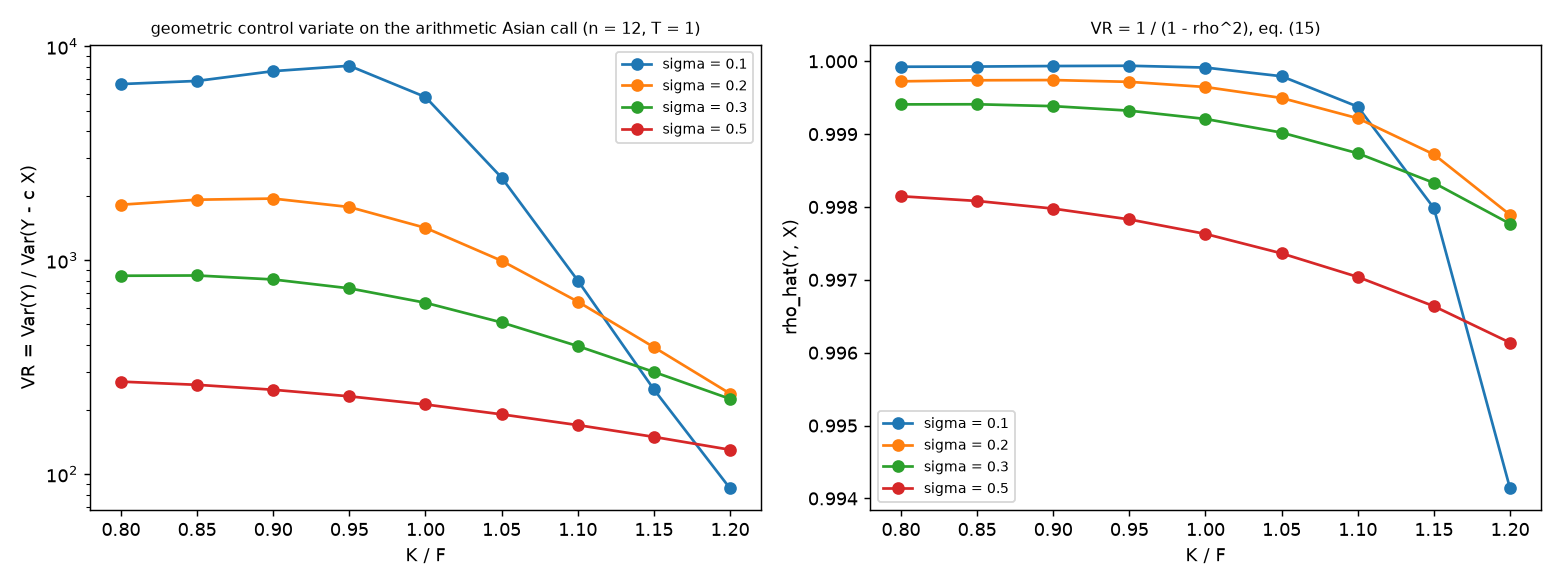
\includegraphics[width=\textwidth]{asian_cv_vr.png}
\caption{Arithmetic Asian call, $n=12$, $T=1$, $2\times10^5$ paths per $\sigma$. Left: the variance-reduction factor
$\mathrm{VR}=\Var(Y)/\Var(Y-\hat cX)$ on a log scale, against $K/F$; right: the estimated correlation
$\hat\rho(Y,X)$.}
\label{fig:asian-cv-vr}
\end{figure}

Figure~\ref{fig:asian-cv-vr} shows VR and $\hat\rho$ for four volatilities; Table~\ref{tab:asian-vr} reports the
at-the-money values ($K/F=1$).
\begin{table}[htbp]
\centering
\small
\caption{Control variate at the money ($K/F=1$, $n=12$, $T=1$, $2\times10^5$ paths).}
\label{tab:asian-vr}
\begin{tabular}{lcccc}
\toprule
$\sigma$ & 0.1 & 0.2 & 0.3 & 0.5\\
\midrule
VR & 5793 & 1416 & 632 & 211\\
$\hat\rho$ & 0.99991 & 0.99965 & 0.99921 & 0.99763\\
$\hat c$ & 1.014 & 1.030 & 1.047 & 1.086\\
\bottomrule
\end{tabular}
\end{table}

The ratios between successive VRs are 4.1, 2.2 and 3.0, against the squared ratios of $\sigma$, 4, 2.25 and 2.8: the
rule $\mathrm{VR}\sim1/\sigma^2$ works well at the money. Away from the money VR collapses, and faster when $\sigma$ is
small: at $\sigma=0.1$ it goes from a maximum of 8113 ($K/F=0.95$) to 85.5 at $K/F=1.2$ ($\hat\rho=0.9941$,
$\hat c=1.12$). This is why one always states \emph{which} $\sigma$ and strike a VR refers to.

\begin{esempio}[title={\texorpdfstring{Example: Fusai--Meucci, arithmetic with $n=12$}{Example: Fusai--Meucci,
arithmetic with n=12}}]
With $2\times10^5$ paths: at $K=100$ the control-variate price is 4.88132 with SE $3.8\times10^{-4}$, against the
published value 4.88210. Plain Monte Carlo on the same paths would have SE $1.5\times10^{-2}$. VR $=1924$, 1608 and 612
at $K=90$, 100, 110 ($\hat\rho=0.99974$, 0.99969, 0.99918). All nine published values ($n=12$, 50, 250) are within
3 SE. A comparison between the control-variate price and plain Monte Carlo on \emph{independent} seeds ($\sigma=0.3$,
$n=12$) gives $\max|z|=0.77$, with SE ratios 28.6, 24.8 and 15.1: the control does not shift the mean.
\end{esempio}

\section{Model-free parity and bounds}
Given the fixing forwards, parity and a few bounds hold in any model.
\begin{itemize}
\item \textbf{Parity.} Since $(A-K)^+-(K-A)^+=A-K$,
\[
C_A-P_A=\DF(\bar A_F-K).
\]
On the same paths it holds exactly with the Monte Carlo mean of $A$ in place of $\bar A_F$.
\item \textbf{Lower bounds for the call.} By Jensen, $\E(A-K)^+\ge(\E A-K)^+$; by AM--GM, $A\ge G$ on every path.
Hence
\[
C_A\ge\DF(\bar A_F-K)^+,\qquad C_A\ge C_G .
\]
\item \textbf{First upper bound.} The function $x\mapsto(x-K)^+$ has slope at most 1, hence
$(A-K)^+\le(G-K)^++(A-G)$. Taking expectations:
\[
C_A\le C_G+\DF(\bar A_F-F_G).
\]
\item \textbf{Second upper bound.} By convexity the call on the average is worth less than the average of the calls:
\[
C_A\le\frac{\DF}{n}\sum_ic_i ,
\]
with $c_i$ the (undiscounted) vanilla on the single fixing. It is a static super-replication with $n$ vanillas of
notional $1/n$.
\item \textbf{Put.} $P_G-\DF(\bar A_F-F_G)\le P_A\le P_G$.
\end{itemize}
These bounds are useful because they catch convention errors (fixing at zero, wrong curve) that a small standard
error would hide. In the project they are tested path by path (to $10^{-12}$) and in expectation (to 3 SE).

\section{Why the control is valid only under Black}
A control variate requires the exact mean \emph{under the law that generated} $X$. Under Heston $G$ is not lognormal,
and in general $\E^H(G-K)^+\ne V_G(\sigma)$ for any $\sigma$.
\begin{attenzione}
Using the Black geometric price as the mean anyway shifts the estimate by $c\,(\E^HX-V_G)$. This shift does not
shrink with $N$, while the standard error stays tiny: the result is ``a wrong number with great confidence''. This is
why the code, if asked for the control under Heston, raises an error instead of returning a price.
\end{attenzione}
Under Heston the default is plain Monte Carlo, which is always valid. The correct alternatives, not implemented
because no test requires them, are:
\begin{itemize}
\item a \textbf{Black shadow path} on the same random numbers: one builds
\[
Z^B=\rho Z_v+\sqrt{1-\rho^2}\,Z_\perp ,
\]
which is exactly $\N(0,1)$ and independent across steps, and simulates a Black path with deterministic variance equal
to the expected Heston variance. Its geometric Asian has an exactly known mean, \eqref{eq:kv}, and is correlated with
the Heston payoff because it uses the same draws;
\item a control with known mean under Heston, for example $A$ itself ($\E A=\bar A_F$, exact with the QE-M scheme) or
a vanilla priced with COS;
\item the geometric Asian under Heston with Fourier methods.
\end{itemize}
In any case a control variate reduces the noise; it never removes the bias of the discretization scheme.

\section{The sub-stepping problem under Heston}
Under Black the simulation is exact at the fixing dates, whatever the spacing: one step per period is enough. Under
Heston it is not. Each interval between two fixings must be split into
\[
m_i=\big\lceil(t_i-t_{i-1})/\Delta_{\max}\big\rceil
\]
equal sub-steps ending exactly on $t_i$, with the QE constants recomputed for each step length.

\begin{progetto}[title={In the qpricer project: a bug found and fixed}]
In the first version the Asian Monte Carlo functions defaulted to a single QE-M step per period between two fixings.
An independent check measured it with quarterly fixings, a published Heston parameter set for the SPX and $3\times10^6$
paths on independent seeds. Default minus step $1/32$:
\[
z=-2.6,\qquad z=-3.6,\qquad z=+5.9\qquad(K=90,\ 100,\ 110),
\]
that is $+0.0133$ (1.3\%) at $K=110$. An independent QE-M scheme with step $1/64$ agreed with step $1/32$ and refuted
the default.

\smallskip
\emph{Why the tests had not seen it.} The Heston tests for the Asian passed the step explicitly, so they never used the
default. \emph{Interpretation.} The error changes sign with the strike: the martingale correction of QE-M keeps
$\E S_t$ exact, so the mean of $A$ was right; a step one quarter long gets the \emph{shape} of the joint law of
$(x,v)$ wrong, not its mean.

\smallskip
\emph{Fix.} The default is now $\Delta_{\max}=1/32$ everywhere (\code{MAX\_DT} in
\path{src/qpricer/engines/exotic_mc.py}), as already for the autocallable. After the fix, with $2\times10^6$ paths,
default against $1/32$ gives $z=-1.08$, $-1.25$, $-1.14$. A regression test checks the default. Lesson: test the
defaults that users actually call.
\end{progetto}

\section{Implementation details}
\begin{itemize}
\item \textbf{Running sums.} Paths are not stored: one accumulates $\Sigma_A\mathrel{+}=F_ke^{x_k}$ and
$\Sigma_L\mathrel{+}=x_k$; at the end $A=\Sigma_A/n$ and $G=\bar G_F\exp(\Sigma_L/n)$. Memory is $O(N)$, not $O(nN)$:
with $n=250$ and $N=10^6$ each path matrix would take 2 GB.
\item \textbf{No products.} The direct product of the prices would overflow ($100^{250}=10^{500}$, beyond the largest
double). $\bar G_F$ is computed as the exponential of the mean of the logarithms.
\item \textbf{Formula on arbitrary dates.} \eqref{eq:sigma-G} is computed in Abel form and checked against the double
sum to $10^{-12}$. For Black the kernel is called with $\sigma=\sigma_G$ and $T=1$: only the product $\sigma\sqrt T$
matters.
\item \textbf{AM--GM in floating point.} With nearly equal fixings $G$ can exceed $A$ by a few ulp: the test
$Y_i\ge X_i$ is done to $10^{-12}$ relative, without truncation.
\end{itemize}

\needspace{8\baselineskip}
\begin{progetto}[title={In the qpricer project: code and results}]
The code:

\noindent{\small\begin{tabularx}{\linewidth}{@{}l>{\raggedright\arraybackslash}X@{}}
\path{src/qpricer/engines/analytic.py} & closed form (\code{geometric\_asian\_price})\\
\path{src/qpricer/engines/exotic_mc.py} & Monte Carlo and control (\code{asian\_mc}, \code{control\_variate})\\
\path{tests/test_asian.py} & tests
\end{tabularx}}
\medskip

\noindent The checks:
\begin{center}
\small
\begin{tabularx}{\textwidth}{>{\raggedright\arraybackslash}Xll}
\toprule
check & measured & threshold\\
\midrule
geometric Monte Carlo vs \eqref{eq:kv}, 39 cells ($\sigma$, $T$, $n$, $K/F$) & $\max|z|=1.90$ & 3 SE\\
mean of $G$ vs $F_G$ and mean of $A$ vs $\bar A_F$ & $\max|z|=1.45$ & 3 SE\\
formula vs Fusai--Meucci table 4 ($n=12$, 50, 250) & $1.28\times10^{-4}$ & $3\times10^{-4}$\\
control vs Fusai--Meucci table 6 & all within 3 SE & 3 SE $+3\times10^{-4}$\\
control vs plain Monte Carlo, independent seeds & $\max|z|=0.77$ & 3 SE\\
Heston $\xi=10^{-4}$, geometric QE-M vs \eqref{eq:kv} & $\max|z|=0.55$ & 3 SE\\
\bottomrule
\end{tabularx}
\end{center}
\end{progetto}

\needspace{6\baselineskip}
\begin{riassunto}
\begin{itemize}
\item Asian = option on the average of the fixings; depends on the whole forward curve.
\item Geometric: $\ln G$ Gaussian $\Rightarrow$ Black with $F_G$ and $\sigma_G$ \eqref{eq:FG}--\eqref{eq:kv};
$\sigma_G^2\to\sigma^2T/3$. Watch the fixing at zero and the continuous formula.
\item Control: $c^*=\Cov/\Var$, $\mathrm{VR}=1/(1-\rho^2)$. Arithmetic and geometric differ at second order: VR from
5793 ($\sigma=0.1$) to 211 ($\sigma=0.5$) at the money, much less away from the money.
\item Model-free bounds: Jensen, AM--GM, slope 1 and convexity.
\item Control valid only under Black: under Heston the Black mean is wrong and the code refuses.
\item Under Heston sub-steps are needed ($\Delta\le1/32$): one step per quarter gave a bias of up to $+1.3\%$.
\end{itemize}
\end{riassunto}

\needspace{6\baselineskip}
\begin{domande}
\begin{enumerate}
\item Why does the geometric Asian have a closed form and the arithmetic one not?
\item Derive $\sigma_G^2$ in the three forms of \eqref{eq:sigma-G} and the limit $\sigma^2T/3$.
\item Why is the forward of $G$ smaller than the geometric mean of the forwards?
\item Derive $c^*$ and the variance-reduction factor. Is the price with estimated $\hat c$ biased?
\item Why does VR fall when $\sigma$ grows and when the strike moves away from the money?
\item What happens if under Heston you use the Black geometric price as a control?
\item A 3 SE test passes with an explicit step but the default is wrong: how do you find out?
\end{enumerate}
\end{domande}

\chapter[The single-underlying autocallable]{The single-underlying\\ autocallable}
\label{cap:autocallable}

The autocallable is one of the structured products most widely sold to retail investors. It is an excellent case
study because it combines digitals, a barrier put and a random maturity, and it shows sharply why the price depends on
the smile and not on the ATM volatility alone. In this chapter we decompose the product, build the closed-form oracles,
design the Black--Heston comparison with common random numbers and report the results with the Heston model calibrated
to the SPX.

\section{The term sheet}
Notional 1; all levels are ratios to a reference level $S_{\text{ref}}$ fixed at issue. Observation dates, period
lengths and fixings are
\[
0<t_1<\dots<t_n=T,\qquad\tau_i=t_i-t_{i-1},\qquad X_i=S_{t_i}/S_{\text{ref}} .
\]
Three barriers: \textbf{autocall} $B_{ac}$, \textbf{coupon} $B_c$, \textbf{protection} $B_p$. Period coupon
$c_i=c\,\tau_i$, with $c$ a simple annual rate. Every test is ``$\ge$'': being exactly on the barrier counts as above.
\begin{itemize}
\item \textbf{Intermediate dates} $t_i<T$: if $X_i\ge B_{ac}$ the product is redeemed early: it pays $1+$coupon and
terminates. Otherwise it pays the coupon if $X_i\ge B_c$.
\item \textbf{Maturity} $T$ (no autocall test): coupon if $X_n\ge B_c$; capital $1$ if $X_n\ge B_p$, otherwise $X_n$,
that is, the investor bears the full loss. The protection is \emph{European}: observed at maturity only.
\item \textbf{Memory}: an unpaid coupon is recovered on the first date on which a coupon is paid.
\end{itemize}
Every cash flow fixed at $t_i$ is paid at $t_i$ and discounted with its own $\DF(t_i)$, with no issuer credit spread.

\begin{progetto}[title={In the qpricer project: the two study term sheets}]
Both with $B_{ac}=1$, $B_c=0.7$, $B_p=0.6$, memory on, $c=8\%$ per year.
\begin{itemize}
\item \textbf{\mbox{AC-Q}}: quarterly, $t_i=i/4$, $n=6$, $T=1.5$ years, inside the last quoted expiry (1.61 years).
\item \textbf{\mbox{AC-A}}: annual, $t_i=1,2,3$. Beyond 1.61 years carry and Heston are \emph{extrapolated}: the
results must be read with this caveat.
\end{itemize}
The market inputs come from the parity table. $\ln F$ and $\ln\DF$ are interpolated linearly in $T$ and extrapolated
flat beyond the last expiry. The reference level is
\[
S_{\text{ref}}=F_0(T_{(1)})\,\DF(T_{(1)})=7374.4255
\]
(first expiry: spot minus the present value of the dividends up to there). For \mbox{AC-Q} the ratios
$f_i=F_0(t_i)/S_{\text{ref}}$ range from 1.00994 to 1.06105 and the $\DF_i$ from 0.98774 to 0.92872. The rate $c=8\%$
is used only for pricing: the fair coupon is computed separately.
\end{progetto}

\section{Cash flows on a path}
With an ``still alive'' indicator $A_i$ (starting at 1), a memory $U_i$ of unpaid coupons (starting at 0) and
$m\in\{0,1\}$ the memory flag:
\begin{align}
\chi_i&=A_i\,\ind\{X_i\ge B_{ac}\}\quad(i<n),\qquad\chi_n=0,\qquad A_{i+1}=A_i-\chi_i,\\
\pi_i&=A_i\,\ind\{X_i\ge B_c\},\qquad C_i=\pi_i\,(c_i+m\,U_i),\qquad U_{i+1}=(1-\pi_i)(c_i+m\,U_i),\\
R_i&=\chi_i\quad(i<n),\qquad R_n=A_n\big[1-(1-X_n)\,\ind\{X_n<B_p\}\big],\\
\mathrm{PV}&=\sum_i\DF_i\,(C_i+R_i),\qquad V=\E[\mathrm{PV}].\label{eq:ac-pv}
\end{align}
The order of operations matters: on each date the coupon (with memory) is computed first, then the autocall test, and
the cash flows are multiplied by $A$ \emph{before} it is updated. In this way nothing is paid twice. On an autocall date
$X_i\ge B_{ac}\ge B_c$, so an early redemption always pays the coupon as well.

\begin{esempio}[title={\texorpdfstring{Example: a path by hand (\mbox{AC-Q}, $c_i=0.02$)}{Example: a path by hand
(AC-Q, c\_i=0.02)}}]
$X_1=0.65<0.70$: no coupon, which goes into memory. $X_2=0.80$: pays $c_1+c_2=0.04$. $X_3=1.01\ge1$: redemption, pays
$1+0.02$ and terminates. If instead the path reaches maturity, a final fixing $X_6=0.65$ ($\ge0.6$ but $<0.7$) repays 1
with no coupon, while $X_6=0.40$ repays 0.40.
\end{esempio}

\paragraph{Linearity in the coupon and par coupon.} No indicator depends on $c$, which enters only through
$c_i=c\tau_i$. Hence the PV is \emph{affine} in $c$ path by path:
\begin{equation}
\mathrm{PV}_j=a_j+c\,b_j,\qquad
\hat c=\frac{1-\bar a}{\bar b},\qquad
\SE(\hat c)=\frac{s(a_j+\hat c\,b_j)}{\sqrt N\,\bar b}.
\end{equation}
The ``par'' coupon (price 1) is obtained from a single set of paths, with no root search on noisy prices; the standard
error comes from the delta method.

\section{What the investor has bought}
\subsection{The decomposition}
\noindent\textbf{Step 1 (the capital).} The redemption at maturity can be rewritten as
\[
\ind\{X\ge B_p\}+X\,\ind\{X<B_p\}=1-(1-X)\,\ind\{X<B_p\}.
\]

\noindent\textbf{Step 2 (put plus digitals).} For $B_p\le1$, on the event $\{X<B_p\}$ we have
$1-X=(B_p-X)+(1-B_p)$, hence
\[
(1-X)\,\ind\{X<B_p\}=(B_p-X)^++(1-B_p)\,\ind\{X<B_p\}:
\]
a put struck at $B_p$ plus $(1-B_p)$ \emph{digital puts} at the same strike.

\noindent\textbf{Step 3 (grouping).} Grouping the ``1'' terms by redemption date gives a bond maturing at the random
date $\tau^\star$ (autocall, or $T$):
\begin{proposizione}[Decomposition]
\begin{equation}\label{eq:ac-scomposizione}
\begin{split}
V={}&\underbrace{\E[\DF(\tau^\star)]}_{\substack{\text{bond with}\\\text{random maturity}}}
+\underbrace{\sum_i\DF_i\,\E[C_i]}_{\text{coupon digitals}}\\
&-\underbrace{\DF_n\,\E\big[A_n(1-X_n)\,\ind\{X_n<B_p\}\big]}_{\text{down-and-in put, if still alive}} .
\end{split}
\end{equation}
\end{proposizione}
Since $A_n\le1$, the embedded put is worth at most the European down-and-in put
\begin{equation}\label{eq:dip}
\mathrm{DIP}_E=\DF_n\big[p_n(B_p)+(1-B_p)\,D_n^-(B_p)\big],\qquad D_n^-(k)=\Q(X_n<k),
\end{equation}
with $p_n(k)=\E(k-X_n)^+$. This piece is \textbf{static and model-free}: given the smile at maturity $T$, it is a put
plus $0.4$ digital puts at 60\%.

\begin{idea}[title={Who is long what}]
The \textbf{investor} is long the bond and the coupon digitals, and \textbf{short} a 60\% down-and-in put: they have
sold the issuer protection against crashes, and this is what funds high coupons. They are short volatility and short
the downside. The \textbf{issuer} holds the opposite position: long the put, short the digitals and the bond. At issue
it is long vega. When the market falls its vega grows, reaches a maximum above the barrier and then changes sign,
because close to maturity the put becomes an in-the-money digital (``peak vega''). Issuers hedge by selling
volatility: autocallable issuance is a steady supply of volatility to the market.
\end{idea}

\subsection{The sign of vega: clear without autocall, not with it}
With $s$ the total volatility, let
\[
d_\pm(f,L,s)=\frac{\ln(f/L)\pm s^2/2}{s},\qquad
\partial_sd_-=-\frac{\ln(f/L)}{s^2}-\frac12 .
\]
The derivative is negative exactly when $L<f\,e^{s^2/2}$. In that case the ``above'' digital $\Phi(d_-)$ loses value
with volatility and the ``below'' digital $\Phi(-d_-)$ gains value. With positive carry ($f_i\ge1$) this holds for the
coupon digitals at $B_c$, for the autocall digitals at $B_{ac}=1$ and for the put at $B_p$. Hence, \textbf{without
autocall}, $V$ is strictly decreasing in $\sigma$: the investor is short vega. With the autocall there is no general
sign, because volatility also shifts the timing of the redemption (see Section~\ref{sec:ac-vega}).

\section{Why a flat volatility is not enough}
The digital is the derivative of the put with respect to the strike. If the put price is $p_{BS}(k,\sigma(k))$, with a
strike-dependent volatility, the chain rule gives
\begin{equation}\label{eq:digitale-smile}
D^-(k)=\frac{\partial p}{\partial k}
=\underbrace{\Phi(-d_-)}_{\text{Black at level }\sigma(k)}
+\underbrace{k\,\varphi(d_-)\sqrt t\,\sigma'(k)}_{\text{smile slope}} .
\end{equation}
The first term is $\partial_kp_{BS}$, the second is the vega of the put, $k\varphi(d_-)\sqrt t$, times $\sigma'(k)$.
\begin{perche}[title={Why no single volatility prices a digital}]
The price of a digital depends not only on the \emph{level} of the volatility at the strike, but also on the
\emph{slope} of the smile there. With the SPX skew ($\sigma'<0$) the second term matters. Using a single volatility
for everything, the ATM one to boot, is therefore wrong twice over: the 60\% put and the 70\% coupon sit deep in the
skew, where the implied volatility is much higher than ATM.
\end{perche}
The expected sign is therefore $V_{\text{Heston}}<V_{\text{Black}}(\sigma_{\mathrm{ATM}})$. The fatter left tail makes
the put sold by the investor worth more and lowers the probability of being above $B_c$. Near ATM, on the other hand,
with $\sigma'<0$ \eqref{eq:digitale-smile} says that the autocall digital $D^+(1)$ is above its flat value: more early
redemptions.

\section{The closed-form oracles}
Before trusting the Monte Carlo on the full product, one checks cases that can be computed exactly.
\begin{itemize}
\item \textbf{No autocall and no memory} ($B_{ac}=\infty$, $m=0$). Each cash flow depends on a single fixing, so the
value is a sum of marginals:
\begin{equation}\label{eq:ac-nocall}
V^{nc}=\sum_i\DF_i\,c_i\,D_i^+(B_c)+\DF_n-\mathrm{DIP}_E .
\end{equation}
Under Black
\[
D_i^+(k)=\Phi\big(d_-(f_i,k,s_i)\big),\qquad\mathrm{DIP}_E=\DF_n\big[\Phi(-d_-)-f_n\Phi(-d_+)\big],
\]
with $d_\pm=d_\pm(f_n,B_p,s_n)$. Under Heston puts and digitals come from COS (Chapter~\ref{cap:heston}); the digital
is a central difference from \emph{a single} COS call at the three strikes, so it is the derivative of one series.
\item \textbf{Two dates}, any memory. One conditions on $X_1$: given $X_1=x$, the fixing $X_2$ is lognormal with mean
$g=xf_2/f_1$ and total volatility $s_{1,2}$, so the cash flows at $t_2$ are priced with Black. What remains is a
one-dimensional integral over the law of $X_1$, split at the jump point of the memory ($X_1=B_c$).
\item \textbf{Zero volatility}: $X_i=f_i$ and the term sheet is evaluated by hand.
\item \textbf{Path identities}: the sum of the first-redemption probabilities plus the probability of reaching
maturity equals 1 exactly; the PV is monotonic in $B_c$, $B_p$, $c$ and in the memory.
\end{itemize}

\section{Monte Carlo and common random numbers}
Under Black one exact step per period is enough. Under Heston one uses QE-M with sub-steps $\Delta\le1/32$ that end
exactly on the observation dates.

\subsection{The common-random-numbers design}
We want the \emph{difference} $V_H-V_{BS}$, which is of the order of 1--2\% of the notional. With independent seeds
its variance would be the sum of the two variances. With common random numbers (CRN) it is estimated on the per-path
differences.

\noindent\textbf{Step 1.} At each sub-step $k$ of length $\Delta_k$, QE-M draws independent $(Z_{v,k},Z_{\perp,k})$;
the spot shock is $\rho Z_{v,k}+\sqrt{1-\rho^2}Z_{\perp,k}$, which is $\N(0,1)$.

\noindent\textbf{Step 2.} For period $i$ the Brownian increments are summed and normalized:
\begin{equation}\label{eq:crn}
Z_i=\sum_{k\in\text{period }i}\sqrt{\frac{\Delta_k}{\tau_i}}\,\big(\rho Z_{v,k}+\sqrt{1-\rho^2}\,Z_{\perp,k}\big).
\end{equation}
A sum of independent $\N(0,\Delta_k)$ is $\N(0,\tau_i)$, so $Z_i$ is exactly $\N(0,1)$, and independent across
different periods.

\noindent\textbf{Step 3.} The Black paths are built with these $Z_i$: they are exact GBMs, driven by the Brownian
motion of the Heston spot. The difference $D_j=\mathrm{PV}^H_j-\mathrm{PV}^{BS}_j$ has standard error $s_D/\sqrt N$,
\emph{never} $\sqrt{\SE_H^2+\SE_{BS}^2}$, which holds only for independent estimates.

\begin{attenzione}[title={The gain is modest, and that is fine}]
The digitals limit the correlation: paths close to a barrier change outcome between the two models. On the full
product (calibrated \mbox{AC-Q}) the error of the difference is 0.000217, just below what the separate SEs would give
(0.000229 for Heston, 0.000094 for Black). On the term in which both legs are lognormal the gain is instead large: SE
0.000120 against separate SEs of 0.000163 and 0.000094. The real benefit is consistency: every term of the
decomposition that follows is a per-path difference, so it measures model differences and not noise.
\end{attenzione}

\section{Black versus Heston: the attribution}
Three prices are compared on the same paths:
\begin{itemize}
\item $V_{BS}$: Black with flat volatility $\sigma_{\mathrm{ATM}}$, the Heston implied volatility at the forward and at
maturity $T$. In this way both models price the ATM-forward vanilla at $T$ identically.
\item $V_{TS}$: Black with the Heston expected variance \eqref{eq:var-attesa},
\[
w(t)=\theta t+(v_0-\theta)\,\frac{1-e^{-\kappa t}}{\kappa},
\]
that is, the limit $\xi\to0$.
\item $V_H$: Heston.
\end{itemize}
The superscript ``nc'' denotes the same term sheet without autocall and without memory, priced in closed form with
\eqref{eq:ac-nocall}. The difference decomposes exactly into three terms:
\begin{equation}\label{eq:attribuzione}
\begin{split}
V_H-V_{BS}={}&\underbrace{(V_{TS}-V_{BS})}_{\substack{\text{1: flat }\sigma_{\mathrm{ATM}}\text{ vs}\\\text{variance curve}}}
+\underbrace{(V^{nc}_H-V^{nc}_{TS})}_{\substack{\text{2: marginal smile}\\\text{at }B_p,\,B_c}}\\
&+\underbrace{\big[(V_H-V_{TS})-(V^{nc}_H-V^{nc}_{TS})\big]}_{\text{3: path (forward skew, vol-of-vol)}} .
\end{split}
\end{equation}
\begin{itemize}
\item \textbf{Term 1} compares the flat volatility with the Heston expected-variance curve. It contains a \emph{level}
part ($\sqrt{w(T)/T}$ against $\sigma_{\mathrm{ATM}}$: the Heston ATM implied volatility is below the square root of
the expected variance because of the vol-of-vol) and a \emph{shape} part.
\item \textbf{Term 2} is the difference of two closed forms, so it has no standard error. It measures the smile at the
barriers: the Heston put and digitals against those of a lognormal with the same variance.
\item \textbf{Term 3} is the residual. Every coupon and the put pay only on paths not yet redeemed, that is, paths
that stayed below 100\%. The price therefore depends on the future \emph{conditional} distribution (the forward skew),
which Heston generates and Black does not.
\end{itemize}
Since term 3 is defined as a residual, the sum adds back to the difference by construction: this is not a test. The
real tests are the legs compared with the closed forms.

\subsection{The results with calibrated Heston}
The parameters come from the calibration of Chapter~\ref{cap:calibrazione} (SPX snapshot, 21 expiries with
$T\ge0.1$): $\kappa=4.575$, $\theta=0.05293$, $\xi=1.648$, $\rho=-0.7518$, $v_0=0.05237$. Table~\ref{tab:ac-risultati} reports the results with $2\times10^5$ paths.
\begin{table}[htbp]
\centering
\small
\caption{Black versus calibrated Heston on the two study term sheets ($2\times10^5$ paths; CRN standard errors in
brackets).}
\label{tab:ac-risultati}
\begin{tabularx}{\textwidth}{>{\raggedright\arraybackslash}Xll}
\toprule
& \mbox{AC-Q} (1.5 years) & \mbox{AC-A} (3 years, extrapolated)\\
\midrule
$\sigma_{\mathrm{ATM}}$ (Heston) / $\sqrt{w(T)/T}$ & 18.85\% / 22.99\% & 19.72\% / 23.00\%\\
$V_{BS}$ & 1.014530 & 1.021479\\
$V_{TS}$ & 1.006324 & 1.002757\\
$V_H$ & 0.995842 & 0.996342\\
difference $V_H-V_{BS}$ (CRN SE) & $-0.018688$ (0.000217) & $-0.025137$ (0.000342)\\
1: flat $\sigma_{\mathrm{ATM}}$ vs variance curve & $-0.008206$ (0.000120) & $-0.018722$ (0.000163)\\
2: marginal smile (exact) & $-0.020445$ & $-0.014800$\\
3: path & $+0.009963$ (0.000216) & $+0.008386$ (0.000364)\\
par coupon Black / Heston & 5.60\% / 8.93\% & 6.58\% / 8.29\%\\
coupon difference (SE) & $+3.33\%$ (0.05\%) & $+1.71\%$ (0.03\%)\\
$P$(redemption at $t_1$) Black / Heston & 0.5222 / 0.6814 & 0.5395 / 0.6755\\
$P$(never redeemed) Black / Heston & 0.2164 / 0.1371 & 0.3273 / 0.2247\\
expected life Black / Heston & 0.643 / 0.503 years & 1.788 / 1.549 years\\
\bottomrule
\end{tabularx}
\end{table}


\begin{figure}[htbp]
\centering
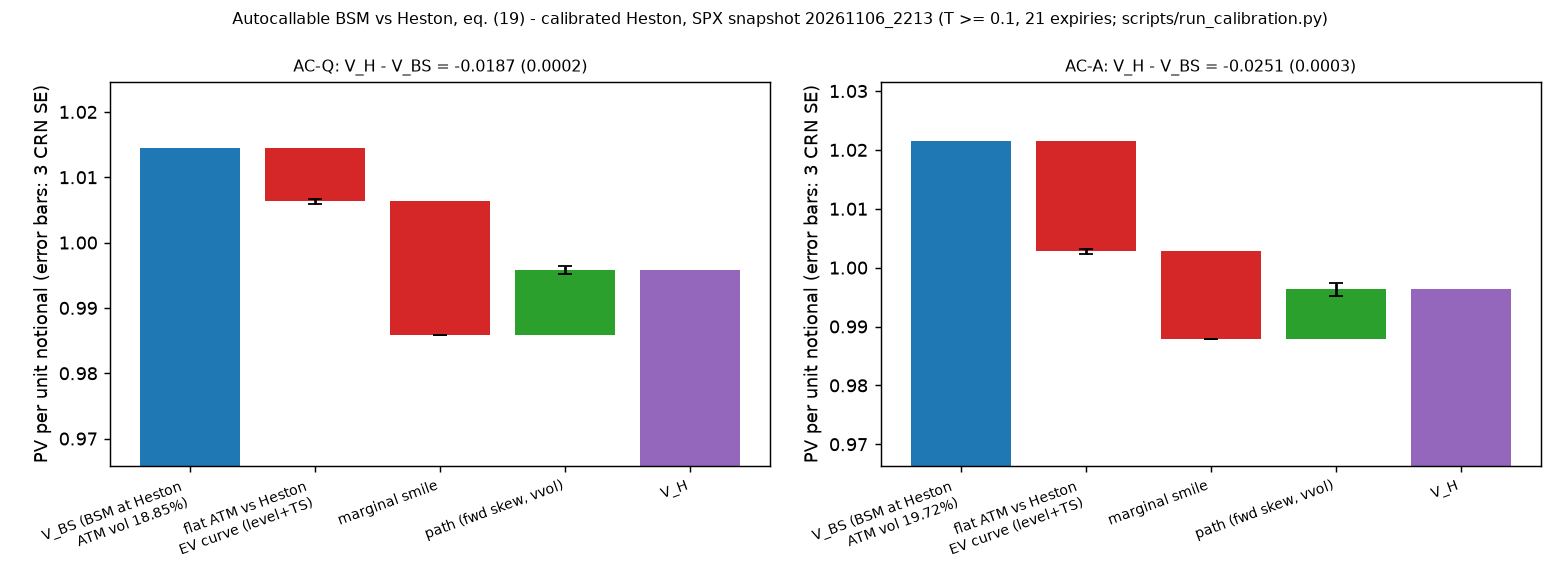
\includegraphics[width=\textwidth]{autocall_attribution_heston_fit_20261106_2213.png}
\caption{Attribution \eqref{eq:attribuzione} with Heston calibrated to the SPX, for \mbox{AC-Q} (left) and
\mbox{AC-A} (right). From the left: $V_{BS}$ at the Heston ATM volatility, the three terms (error bars at 3 CRN SE)
and $V_H$.}
\label{fig:ac-attribuzione}
\end{figure}

\paragraph{How to read them.} Figure~\ref{fig:ac-attribuzione} shows the waterfall. On \mbox{AC-Q} Heston is worth
1.87\% of notional less than Black, in the expected direction.
\begin{itemize}
\item \textbf{Term 2} dominates ($-0.0204$): it is the skew at the 60\% and 70\% barriers. The left tail makes the
issuer's put more expensive and the coupons less likely.
\item \textbf{Term 1} ($-0.0082$) is almost all level: $v_0\approx\theta$, so the curve $w(t)/t$ is almost flat, and
the difference between 22.99\% and 18.85\% is the vol-of-vol effect, very large in the fit ($\xi=1.65$).
\item \textbf{Term 3} is positive ($+0.0100$) and offsets about a third of the rest. It also contains the fact that the
product without autocall suffers the smile penalty on all paths, while the product with autocall suffers it only on
the surviving ones.
\item Heston redeems much more often on the first date (68\% against 52\%): with $\sigma'<0$ the ATM digital is above
its flat value. The expected life shortens.
\item The \textbf{par coupon} rises from 5.60\% to 8.93\%: a flat ATM volatility would make the issuer offer a coupon
more than 3 points too low.
\end{itemize}

\paragraph{Which volatility for Black?} The choice of $\sigma_{\mathrm{ATM}}$ matters, and this is why sensitivity rows
are reported (\mbox{AC-Q}, Table~\ref{tab:ac-sens}).
\begin{table}[htbp]
\centering
\small
\caption{Sensitivity of $V_{BS}$ (\mbox{AC-Q}) to the volatility chosen for Black.}
\label{tab:ac-sens}
\begin{tabularx}{\textwidth}{Xrr}
\toprule
Black volatility & $\sigma$ & $V_{BS}$\\
\midrule
Heston ATM at the forward (the reference leg) & 18.85\% & 1.014530\\
market ATM interpolated at 1.5 years & 18.29\% & 1.015253\\
Heston at the strike $S_{\text{ref}}$ & 20.37\% & 1.012036\\
Heston at the barrier $B_pS_{\text{ref}}$ & 31.79\% & 0.977950\\
\bottomrule
\end{tabularx}
\end{table}

The Heston fit sits about 0.65 vol points above the market ATM on the last expiry (18.94\% against 18.29\%). At the
market ATM volatility $V_{BS}$ rises by 0.000723 (about 3.3 CRN SE of the difference) and the difference with Heston
becomes $-0.019411$: the conclusion does not change. Black at the barrier volatility instead overshoots
($0.977950<V_H$): that volatility prices the put, but the coupons and redemptions sit at other strikes, and the digital
also needs the slope. On \mbox{AC-A} the market ATM volatility is not available (no quoted expiry beyond 1.61 years);
the other two rows give 1.011832 (21.47\%) and 0.967614 (28.36\%).

\begin{progetto}[title={In the qpricer project: checks on the calibrated comparison}]
\begin{itemize}
\item Black and deterministic-variance legs on the CRN paths, restricted to the first two dates, against the two-date
formula: $\max|z|=0.20$ (\mbox{AC-Q}) and 0.72 (\mbox{AC-A}). No-autocall legs on the paths against
\eqref{eq:ac-nocall}: $\max|z|=0.87$ and 1.19.
\item An independent check recomputed everything with its own methods: exact value of $V_{BS}$ by backward induction
1.014493 (project Monte Carlo at $z=0.40$); $V_H=0.995882$ with its own QE-M scheme (project at $z=-0.16$); difference
$-0.018611$; term 2 within $4\times10^{-10}$. With step $1/256$ $V_H=0.995905$: no step bias.
\item Effect of a small known inconsistency: $S_{\text{ref}}$ uses the discount factor of the first expiry from
parity, which is slightly biased; with the smoothed curve $S_{\text{ref}}$ would rise by 0.074\%. The measured effect
on the \mbox{AC-Q} difference is $-8\times10^{-5}$, that is 0.4 CRN SE.
\end{itemize}
\end{progetto}

\section{No single sign for vega}
\label{sec:ac-vega}
Without autocall the product is strictly decreasing in $\sigma$ (tested in closed form). On the full product it is not.
A grid of $\sigma$ under Black, with common random numbers across grid points, gives the values of Table~\ref{tab:ac-vega}.
\begin{table}[htbp]
\centering
\small
\caption{Value of the two autocallables under Black as the flat volatility $\sigma$ varies.}
\label{tab:ac-vega}
\begin{tabular*}{\textwidth}{@{\extracolsep{\fill}}lccccccc@{}}
\toprule
$\sigma$ & 0.10 & 0.15 & 0.20 & 0.25 & 0.30 & 0.35 & 0.40\\
\midrule
$V$ (\mbox{AC-Q}) & 1.01730 & 1.01773 & 1.01271 & 1.00072 & 0.98433 & 0.96618 & 0.94767\\
$V$ (\mbox{AC-A}) & 1.04433 & 1.04008 & 1.01997 & 0.98996 & 0.95633 & 0.92251 & 0.88936\\
\bottomrule
\end{tabular*}
\end{table}

It is a pure Black computation on the market inputs, in which no Heston parameter plays any role. On \mbox{AC-Q} the
value \emph{rises} from $\sigma=0.10$ to $0.15$ ($+0.00043$, SE of the difference 0.00004) and then falls. On
\mbox{AC-A} it is monotonic.
\begin{perche}[title={Why vega changes sign}]
It is a timing effect. For $\sigma\to0$ the \mbox{AC-Q} product is redeemed with certainty on the first date, because
$f_1=1.00994\ge1$. A little volatility delays the redemption, and the investor collects for longer an 8\% coupon,
higher than the fair one, before the put starts to weigh. Only with more volatility does the sold put prevail. Hence
``the autocallable is short vega'' is true for the investor on the product without autocall, not in general.
\end{perche}

\section{A published value that does not reproduce}
Deng, Mallett and McCann (2011), ``Case 2'': monthly dates for one year, $B_{ac}=B_c=1.02$, memory, accrual coupons
$c_j=e^{0.092t_j}-e^{0.092t_{j-1}}$, European protection $B_p=0.8$, $\sigma=20\%$, $F_0(t)=100e^{0.04t}$,
$\DF(t)=e^{-0.06t}$ (the discount factor includes the issuer's CDS spread).
\begin{itemize}
\item Project Monte Carlo: 97.508 (SE 0.009, $10^6$ paths).
\item Exact value, computed independently by backward induction: 97.507 (between the two, $z=+0.09$).
\item Published value (explicit finite differences): \textbf{98.39}, about 100 SE away.
\end{itemize}
The rest of the paper, on the other hand, does reproduce: ``Case 1'' (without autocall) gives roughly par (99.976),
and the first-redemption probabilities of their table 1 match ($\max|z|=2.11$; the first one, $p_1=0.3767$, can also
be derived by hand). Two independent implementations agree with each other and not with the published value. The
possible causes are a different coupon or protection convention in the paper, or the finite-difference error, whose
accuracy the paper does not state. Nothing was adjusted to make it match; the value is not used as an oracle.

\section{Model risk}
\begin{itemize}
\item \textbf{What the vanillas pin down.} Today's vanilla prices pin down the marginals: the European down-and-in put
is a put plus digitals from the smile at $T$ \eqref{eq:dip}, and this is term 2. They do not pin down term 3: coupons
and put pay only on paths that stayed below 100\%, so the price depends on the \emph{forward} skew, driven by
vol-of-vol and spot--vol correlation.
\item \textbf{Heston cannot move it on its own.} In Heston $\xi$ and $\rho\xi$ are fixed by the vanilla fit. Two models
calibrated to the same prices (local volatility, whose forward skew is flat, and stochastic volatility) can give
different prices: this is model risk, which a local-stochastic volatility model would make it possible to control.
\item \textbf{Extrapolation.} \mbox{AC-A} goes beyond the last quoted expiry: carry and Heston are extrapolated.
\item \textbf{Credit and Greeks.} No issuer spread in the discounting. The Greeks are unstable, because the payoff is
made of digitals: pathwise derivatives lose the Dirac terms, and finite differences have a variance that grows like
$1/h$. Dedicated methods are needed (likelihood ratio, digital smoothing), outside the scope of the project.
\end{itemize}

\begin{progetto}[title={In the qpricer project: code and checks}]
The code:

\noindent{\small\begin{tabularx}{\linewidth}{@{}l>{\raggedright\arraybackslash}X@{}}
\path{src/qpricer/products.py} & cash flows (\code{autocall\_flows})\\
\path{src/qpricer/engines/exotic_mc.py} & Monte Carlo and CRN (\code{autocall\_mc}, \code{fixings})\\
\path{src/qpricer/engines/analytic.py} & oracles (\code{autocall\_nocall}, \code{autocall\_two\_dates})\\
\path{scripts/autocall_compare.py} & Black--Heston comparison\\
\path{tests/test_autocallable.py} & tests
\end{tabularx}}
\medskip

\noindent The checks:
\begin{itemize}
\item Black Monte Carlo against the closed forms (no autocall, $n=1$, two dates with and without memory):
$\max|z|=1.79$.
\item Heston: mean of $M_t$ equal to 1, digitals against COS, product without autocall against COS: $\max|z|=1.32$.
\item Heston with $\xi=10^{-4}$ against Black at the discrete QE variance, same draws: $|z|=0.18$.
\item Cash flows identical (within $10^{-15}$) to an independent path-by-path transcription, on $20{,}000$ paths and
seven term-sheet variants, with exact ties at every barrier.
\item Full product under Black against an independent exact value, 18 cases: $\max|z|=2.36$.
\end{itemize}
\end{progetto}

\needspace{6\baselineskip}
\begin{riassunto}
\begin{itemize}
\item Autocallable = random-maturity bond + coupon digitals $-$ 60\% European down-and-in put.
\item The investor is short the put and short the downside; the issuer is long vega at issue (``peak vega'' above the
barrier). Without autocall the investor is short vega; with the autocall there is no single sign.
\item Digitals depend on the smile slope: no single volatility prices them.
\item PV affine in the coupon $\Rightarrow$ par coupon from a single set of paths.
\item CRN: Black driven by the Heston spot shocks; SE always from the per-path differences.
\item With calibrated Heston (\mbox{AC-Q}): $V_H-V_{BS}=-0.0187$, of which smile at the barriers $-0.0204$; fair coupon
from 5.60\% to 8.93\%. The path term is model risk.
\end{itemize}
\end{riassunto}

\needspace{6\baselineskip}
\begin{domande}[before skip=6pt plus 8pt]
\begin{enumerate}
\item Decompose an autocallable into simple instruments. Who is long vega?
\item Derive the decomposition of the capital into a put plus digitals.
\item Why is the ATM volatility not the relevant one? What does the smile slope add to a digital?
\item Why is the par coupon obtained without a root search?
\item Show that the $Z_i$ of \eqref{eq:crn} are independent $\N(0,1)$. Why is the SE of the difference not
$\sqrt{\SE_H^2+\SE_{BS}^2}$?
\item What does each term of \eqref{eq:attribuzione} measure? Which one is not pinned down by today's vanillas?
\item Why is the \mbox{AC-Q} product worth more at $\sigma=0.15$ than at $\sigma=0.10$?
\item A published value is 100 SE away from yours and from an independent computation: what do you do?
\end{enumerate}
\end{domande}


\part{Calibration, benchmark and validation}
\chapter{Calibration to the SPX surface}
\label{cap:calibrazione}

This chapter fits two models to the SPX implied-volatility surface (snapshot of 6 November 2026, 22:13): a single
Heston parameter set for the whole surface and one SABR per expiry. Before the real data, we check on synthetic data,
with tolerances fixed in advance, that the procedure recovers known parameters. At the end we check that the surface
contains no static arbitrage. Code: \code{src/qpricer/calibration.py}; numbers: \code{scripts/run\_calibration.py} and
\code{scripts/phase5\_gates.py}.

\section{What calibrating means}
Calibrating means choosing the parameters $p$ so that the model reproduces the market as closely as possible. It is a
\textbf{nonlinear least-squares} problem:
\begin{equation}\label{eq:cal-ls}
\hat p=\arg\min_p\ \tfrac12\sum_{i=1}^n r_i(p)^2 ,
\end{equation}
where $r_i$ is the weighted \emph{residual} of quote $i$ and $\tfrac12\sum_ir_i^2$ is the \emph{cost}. Three
questions organize the chapter: \emph{what} is compared and with what weight; \emph{how} the model is computed inside
the optimizer without numerical error disturbing the search; \emph{how far} the result can be trusted.

\section{The targets}
\subsection{Bid, ask and mid volatilities}
We start from the OTM surface of Chapter~\ref{cap:dati}: 7625 quotes on 39 expiries, from $T=0.019$ to $T=1.61$
years. The discount factors of the short expiries have already been replaced with a rate curve and the forwards
re-estimated (Section~\ref{sec:breve-termine}).

For each quote $i$ the bid, ask and mid are inverted with Black, and the \textbf{half-spread in volatility}
$h_i=\tfrac12(\sigma^a_i-\sigma^b_i)$ is defined. For an OTM option the intrinsic value is zero, so the bid volatility
exists as soon as the bid is positive.

Notation:
\[
k=\ln(K/F),\qquad s=\sigma\sqrt T,\qquad d_1=-\frac ks+\frac s2,\qquad d_2=d_1-s .
\]
The model prices are \emph{normalized} ($F=\DF=1$, strike $e^k$): Heston and SABR with $\beta=1$ depend only on
$K/F$. The normalized vega is $\vega=\varphi(d_1)\sqrt T$.

\subsection{Delta band and thinning}
A quote enters if the mid volatility exists, if the mid is worth at least 0.50 (10 minimum SPX ticks) and if
$|d_1(\sigma^m_i)|\le z_5=\Phi^{-1}(0.95)=1.6449$, that is, between the 5-delta put and call. Beyond 5$\Delta$ the
options are worth a few ticks, the spread is a large fraction of the price and the volatility is almost undetermined.

Then we \textbf{thin}: 25 targets equally spaced in $d_1$ between $-z_5$ and $z_5$ are fixed, for each one the
not-yet-used quote with the closest $d_1$ is taken, and the put and the call closest to $k=0$ are always added. Each
expiry thus has 25--27 quotes.

\begin{perche}[title={Why thin, and why 25}]
\begin{itemize}
\item A smile within the band has about 4--5 ``shape numbers'' (level, slope, curvature, wing slopes): 25 points give
at least 5 per number.
\item Adjacent strikes 5 points apart differ by $\Delta k\approx7\times10^{-4}\ll s$: they are quoted by the same
market maker and their errors are not independent. They add weight, not information. Targets 0.14 apart in $d_1$ make
the independent-errors assumption on which the error bars rest more credible.
\item Without thinning, the weeklies (hundreds of strikes) would dominate the sum \eqref{eq:cal-ls}.
\end{itemize}
\end{perche}

\subsection{The Heston window}
Heston is calibrated only on the 21 expiries with $T\ge0.1$; the 18 shortest are left \textbf{out of sample}. The
reason, derived in Section~\ref{sec:cal-skew}, is that Heston has a single time scale, $1/\kappa$, and cannot
reproduce both the skew of the weeklies and that of the long expiries. We fit the expiries that matter for the
autocallable (0.1--1.6 years) and \emph{measure} the error on the others. SABR is calibrated on all expiries, one at a
time.

\begin{progetto}[title={In the qpricer project: the targets}]
7625 OTM quotes $\to$ 5806 in the band $\to$ 1029 after thinning $\to$ 565 Heston residuals on the 21 expiries with
$T\ge0.1$, plus 464 out-of-sample quotes. Functions \code{in\_band} and \code{thin}.
\end{progetto}

\section{The objective function}
\subsection{Volatility residuals}
The Heston residual is
\begin{equation}\label{eq:cal-res}
r_i(p)=w_i\big[\sigma^H_i(p)-\sigma^m_i\big],\qquad w_i=\frac{1}{\max(h_i,\,h_{\min})},\qquad h_{\min}=0.001 ,
\end{equation}
with $\sigma^H_i$ the implied volatility of the Heston price. With this weight $|r_i|\le1$ means that the model is
\emph{inside} the bid/ask. The \textbf{floor} $h_{\min}$ (0.1 vol points) prevents the very tight quotes from
dominating: it is active on 60.9\% of the thinned quotes (median half-spread 0.078 vol points).

\subsection{Equivalence with vega-weighted prices}
\noindent\textbf{Step 1.} With $\Delta=\sigma^H-\sigma^m$, expand the normalized Black price in $\sigma$:
\[
v(\sigma^H)-v(\sigma^m)=\vega^m\Delta+\tfrac12\,\partial_\sigma\vega^m\,\Delta^2+O(\Delta^3).
\]
\noindent\textbf{Step 2.} Differentiating $\vega=\varphi(d_1)\sqrt T$ gives $\partial_\sigma\vega/\vega=d_1d_2/\sigma$,
with $d_1d_2=k^2/s^2-s^2/4$.

\noindent\textbf{Step 3.} Dividing by $\vega^m$:
\begin{equation}\label{eq:cal-prezzo-vol}
\frac{v^H-v^m}{\vega^m}=\Delta\Big[1+\frac{d_1d_2}{2\sigma^m}\,\Delta\Big]+O(\Delta^3).
\end{equation}
\noindent\textbf{Step 4.} At first order the price residual divided by vega \emph{is} the volatility residual:
minimizing $\sum w_i^2\Delta_i^2$ is equivalent to weighting the price errors by $w_i^2/(\vega^m_i)^2$. The Jacobians
also coincide at first order, so near the optimum the minimum and the standard errors are the same. At the edge of
the band, with $\sigma=0.2$ and $\Delta=0.3$ vol points, the correction is about 2\% (estimate).

\begin{perche}[title={Why volatilities, then}]
Far from the optimum $\Delta$ is not small: in the wings $d_1d_2$ is large and the price is convex and steep in
$\sigma$, so the price residuals blow up and dominate the first iterations. Volatility residuals stay bounded, and the
quantity to report at the end is precisely a volatility error.
\end{perche}

\subsection{The fallback}
With extreme trial parameters the Heston price may not be invertible (too small, or set to zero because the strike
falls outside the COS interval). A \code{NaN} would stop the optimizer. On those quotes the first-order equivalent
residual is used instead:
\begin{equation}\label{eq:cal-ripiego}
r_i=w_i\,\frac{v^H_i-v^m_i}{\vega^m_i},\qquad \vega^m_i\ \text{computed at } \sigma^m_i .
\end{equation}
The market vega always exists. Fallbacks are counted; at the optimum there are none.

\begin{progetto}
\code{heston\_residuals} forms \eqref{eq:cal-ripiego} and replaces it with \eqref{eq:cal-res} where the inversion
succeeds; with \code{kind="price"} it returns price residuals only. Started from the same points, this second objective
function ends up within 0.83 standard errors of the optimum on the real data (0.48 on the synthetic data S1): the
numerical confirmation of \eqref{eq:cal-prezzo-vol}.
\end{progetto}

\section{COS inside an optimizer}
\subsection{\texorpdfstring{Why freeze $(N,L)$}{Why freeze (N,L)}}
The self-checking COS of Chapter~\ref{cap:heston} chooses $(N,L)$ by itself, and the choice depends on $p$: the price
is a \emph{piecewise} function of the parameters, with jumps of the order of $10^{-9}F$. The optimizer estimates the
Jacobian with finite differences of relative step $10^{-6}$. If the step crosses a level change, it measures the jump
and not the slope: an error of about $10^{-9}/10^{-6}=10^{-3}$ on the derivative (estimate), erratic steps, premature
stops.

So $(N,L)$ is frozen for the whole fit, and $r(p)$ becomes smooth. But the fixed value must be accurate
\emph{wherever} the optimizer may go, that is, over the whole constraint box.

\subsection{The a-priori budget}
Before the fit a criterion is fixed: a \textbf{price error in units of market vega},
\begin{equation}\label{eq:cal-budget}
e_{\vega}=\max_i\frac{\big|v^{\mathrm{COS}}_i-v^{\mathrm{Lewis}}_i\big|}{\vega^m_i}\le10^{-5},
\end{equation}
with Lewis as the independent reference. By \eqref{eq:cal-prezzo-vol} it is the first-order volatility error
\emph{where the model is close to the market}, the only place where an error moves the optimum; it has the scale of
the fallback and is defined even where the model volatility does not exist. $10^{-5}$ is 0.001 vol points: 37 times
below the smallest half-spread, 100 times below $h_{\min}$. It is checked on the 565 Heston quotes at the 32 vertices
of the box and at 128 interior Sobol points.

Pairs tried: $(8192,48)$ gives $3.7\times10^{-5}$ and $(16384,80)$ gives $2.0\times10^{-5}$, both over budget;
$(16384,64)$ gives $9.21\times10^{-6}$ and is chosen. The worst vertex is
\[
(v_0,\kappa,\theta,\xi,\rho)=(0.01,\,0.5,\,0.01,\,3,\,-0.99).
\]
Freezing $(N,L)$ per expiry would save less than 10\%: it is the long expiries that need more terms.

\begin{attenzione}[title={The budget is not a volatility accuracy}]
At the worst vertex the direct error $|\sigma^{\mathrm{COS}}-\sigma^{\mathrm{Lewis}}|$ is $2.48\times10^{-3}$, and
over the whole box it reaches $6.41\times10^{-3}$: only at the vertices with $\xi=3$, $\rho=-0.99$ and on the OTM
calls. There the model volatility is 2--5\% against the market's 13--15\%, and the model vega is $10^{-4}$ to
$10^{-11}$ times the market one: a tiny price error becomes a large volatility error, on a residual that is worth
about 10 vol points anyway. The volatility accuracy that matters is the one at the optimum, checked after the fit.
\end{attenzione}

\subsection{Why the box was narrowed}
The initial design had $v_0,\theta\in[10^{-4},1]$, $\kappa\in[10^{-3},20]$, $\xi\in[0.01,5]$ and COS fixed at
$(1024,12)$. The check against Lewis refuted it.
\begin{itemize}
\item At a plausible point, $(0.03,2,0.04,1,-0.7)$, $L=12$ gives a volatility error of $9.9\times10^{-5}$ ($L=18$:
$9.8\times10^{-7}$).
\item On the original box no fixed pair up to $(4096,30)$ is accurate, and at 4 vertices ($v_0=\theta=10^{-4}$,
$\xi=5$) even the Lewis quadrature fails.
\item The difficult region has small $v_0,\theta$, small $\kappa$ and large $\xi$: $\ln(F_T/F)$ is extremely
leptokurtic, and COS ends up requiring $L\approx80$ with $N=16384$.
\end{itemize}
The production box is
\begin{equation}\label{eq:cal-box}
v_0,\theta\in[0.01,\,0.25],\quad \kappa\in[0.5,\,20],\quad \xi\in[0.01,\,3],\quad \rho\in[-0.99,\,0],
\end{equation}
that is, volatilities between 10\% and 50\%. $\kappa\ge0.5$ is also the edge of the identifiable region
($\kappa T_{\max}\approx0.8$), and with $\rho\le0$ the condition $\kappa-\rho\xi>0$ holds everywhere.

\begin{attenzione}[title={Isn't narrowing the constraints cheating? The check}]
The fit was repeated on the \emph{original} box, with the same pair $(16384,64)$, from 16 Sobol points and from 4
hostile starts (for example $v_0=\theta=10^{-3}$ with $\xi=4.5$, or $\kappa=0.01$). \textbf{20 starts out of 20} reach
the same $\hat p$ (cost equal to $4.7\times10^{-15}$ relative), and $\hat p$ lies \textbf{at least 38 standard errors
inside} the narrowed constraints. An independent check with its own pricer obtained the same. The narrowing does not
move the result; the check is re-run with \code{scripts/run\_calibration.py -{}-box note}.
\end{attenzione}

\begin{progetto}[title={In the qpricer project: frozen COS}]
After the fit COS and Lewis agree in volatility to $4.9\times10^{-13}$ on the 565 in-sample quotes and to
$7.0\times10^{-13}$ on the 464 out-of-sample ones. One residual evaluation costs 87\,ms; the fit with 16 starts takes
29.4\,s on 8 processes.
\end{progetto}

\section{The solver and the error bars}
\subsection{Trust region and multi-start}
We use \code{scipy.optimize.least\_squares} with the \textbf{TRF} method: at each step it linearizes
$r(p)\approx r+J\delta p$, minimizes the approximate cost within a ``trust region'' and enlarges or shrinks the region
according to the quality of the approximation; the box constraints are satisfied by construction. The finite-difference
step is $10^{-6}$ relative: the default one ($\approx1.5\times10^{-8}$) would run into the noise of the volatility
inversion ($\approx10^{-13}$), with relative errors on the derivative close to $10^{-4}$ (estimate).
\code{x\_scale='jac'} rescales parameters that differ by a factor of about 100.

We start from $16=2^4$ points of a \textbf{scrambled Sobol} sequence, with a fixed seed and independent of the data, in
the box
\[
\sqrt{v_0},\sqrt\theta\in[0.10,\,0.40],\quad \ln\kappa\in[\ln0.5,\,\ln8],\quad \ln\xi\in[\ln0.2,\,\ln3],\quad
\rho\in[-0.95,\,-0.2].
\]
$\hat p$ is the converged start with the lowest cost; the \textbf{basin} is the set of starts with cost within a
factor $1+10^{-4}$. A single start would not tell whether the minimum is unique.

\subsection{Standard errors from the Jacobian}
\noindent\textbf{Step 1.} Near the optimum $r(\hat p+\delta p)\approx r(\hat p)+J\delta p$.

\noindent\textbf{Step 2.} If the residuals are independent errors with a common variance, the latter is estimated from
the degrees of freedom:
\begin{equation}\label{eq:cal-s2}
s^2=\frac{2\,\text{cost}}{n-5}.
\end{equation}
\noindent\textbf{Step 3.} The normal equations give $\delta\hat p=-(J^\top J)^{-1}J^\top\varepsilon$, hence
\begin{equation}\label{eq:cal-cov}
C=s^2(J^\top J)^{-1},\qquad \SE_j=\sqrt{C_{jj}},\qquad R_{jk}=\frac{C_{jk}}{\SE_j\SE_k}.
\end{equation}
The inverse is computed with the SVD of $J$, discarding zero singular values. The SVD of $J\,\mathrm{diag}|\hat p|$
gives the relative condition number and the \emph{weakest direction}, the combination the data see worst.

\begin{attenzione}
These are \emph{curvature} standard errors: they hold if the model is right, the window is the chosen one and the
errors are independent. They say nothing about misspecification error.
\end{attenzione}

\subsection{Identifiability}
\label{sec:cal-ident}
\paragraph{\texorpdfstring{The $\kappa$--$\theta$ ridge.}{The kappa-theta ridge.}} The average ATM variance up to $T$
is
\begin{equation}\label{eq:cal-vbar}
\bar v(T)=\theta+(v_0-\theta)\frac{1-e^{-\kappa T}}{\kappa T}=v_0+\tfrac12\kappa(\theta-v_0)T-\tfrac16\kappa^2(\theta-v_0)T^2+\dots
\end{equation}
If all expiries have $\kappa T\ll1$, the data see only $v_0$ and the product $\kappa(\theta-v_0)$: the cost is almost
flat along a hyperbola, the \textbf{ridge}. If all have $\kappa T\gg1$, only $\theta$ and $(v_0-\theta)/\kappa$ are
seen. Separating $\kappa$ from $\theta$ requires expiries with $\kappa T\approx1$.

\paragraph{\texorpdfstring{$\rho$--$\xi$ and $\kappa$--$\xi$.}{rho-xi and kappa-xi.}} The skew is first order in
$\rho\xi$, the curvature second order in $\xi$: only the curvature separates $\rho$ from $\xi$. Moreover, for
$\kappa T\gg1$ the skew decays as $\rho\xi/(2\kappa\sqrt\theta\,T)$ (below): the long expiries see $\xi/\kappa$, and
a positive correlation between $\kappa$ and $\xi$ is expected.

\paragraph{Feller.} $\nu_F=2\kappa\theta/\xi^2$ is \emph{reported}, not imposed: it is not a box constraint, and
imposing it would ruin the skew. It does not matter for Fourier, it matters for Monte Carlo (Chapter~\ref{cap:mc}).

\subsection{The Heston ATM skew}
\label{sec:cal-skew}
From Chapter~\ref{cap:heston}, at first order in $\xi$: $V_H=V_B(\bar v)+\rho\xi J\,\partial_x\partial_\Sigma V_B$,
with $J$ from \eqref{eq:J} and $\Sigma=\bar vT$.

\noindent\textbf{Step 1.} Divide the price correction by the vega $\DF F\varphi(d_1)\sqrt T$:
\[
\partial_x\partial_\Sigma V_B=-\frac{\DF F\varphi(d_1)\,d_2}{2\Sigma}
\quad\Longrightarrow\quad
\delta\sigma=-\frac{\rho\xi J\,d_2}{2\Sigma\sqrt T}.
\]

\noindent\textbf{Step 2.} With $d_2=-k/\sqrt\Sigma-\sqrt\Sigma/2$ we have $\partial_kd_2=-1/\sqrt\Sigma$, hence
\begin{equation}\label{eq:cal-skew}
\psi_H(T):=\partial_k\sigma\big|_{k=0}=\frac{\rho\xi J(T)}{2\,\bar v^{3/2}T^2}.
\end{equation}
\noindent\textbf{Step 3.} For $v_0=\theta$, $J=\theta(T-\tau_\kappa)/\kappa$ with
$\tau_\kappa=(1-e^{-\kappa T})/\kappa$, and
\begin{equation}\label{eq:cal-g}
\frac{\psi_H(T)}{\psi_H(0)}=g(\kappa T),\qquad g(x)=\frac{2(x-1+e^{-x})}{x^2}=1-\frac x3+\frac{x^2}{12}-\dots
\end{equation}
For $T\to0$ the skew tends to the \emph{finite} value $\rho\xi/(4\sqrt{v_0})$; for $\kappa T\gg1$, $g\approx2/x$ and
$\psi_H\approx\rho\xi/(2\kappa\sqrt\theta\,T)$ decays as $1/T$.

\begin{idea}[title={Key idea: Heston has a single clock}]
The Heston skew is almost flat for $T\ll1/\kappa$ and decays as $1/T$ beyond: the only scale is $1/\kappa$. The SPX ATM
skew, according to the \emph{literature}, follows instead a power law of about $T^{-0.4}$ (Bayer--Friz--Gatheral
estimate the exponent 0.407 on a 2013 surface; it has not been measured on the project snapshot). If this held here,
from $T=0.019$ to $0.1$ the market skew would roughly double, while that of Heston with $\kappa=3$ would change by about
8\% (estimates). A $\kappa$ large enough to steepen the weeklies would flatten the long expiries.
\end{idea}
\eqref{eq:cal-skew} is first order in $\xi$, and the calibrated $\xi$ is large: it serves to understand the shape in
$T$, not to compute numbers.

\section{The synthetic test}
\subsection{Data and a-priori tolerances}
Data labelled \textbf{synthetic} are generated from true parameters $p^*$, on the actual Heston grid (565 quotes, with
their $k_i$, $T_j$, $w_i$), with noise $\sigma^{\mathrm{obs}}_i=\sigma^H_i(p^*)+\varepsilon_i$,
$\varepsilon_i\sim N(0,\sigma_\varepsilon^2)$, $\sigma_\varepsilon=0.003$. Two sets: \textbf{S1}, the GS set of
Chapter~\ref{cap:heston} ($v_0=\theta=0.0354$, $\kappa=1.3253$, $\xi=0.3877$, $\rho=-0.7165$; Feller violated,
$\nu_F=0.62$), and \textbf{S2} ($0.015,\,3,\,0.04,\,0.4,\,-0.7$; $\nu_F=1.5$). The seeds are fixed and never changed.

``Recovered'' must mean ``within the expected error'', and the expected error is computed at $p^*$, \emph{without} a
fit.

\noindent\textbf{Step 1.} The fit minimizes $\|W^{1/2}(\sigma(p)-\sigma^{\mathrm{obs}})\|^2$ with
$W=\mathrm{diag}(w_i^2)$. With $J_\sigma=\partial\sigma^H/\partial p$ at $p^*$, the linearized normal equations give
\[
\delta p=A^{-1}J_\sigma^\top W\varepsilon,\qquad A=J_\sigma^\top WJ_\sigma .
\]

\noindent\textbf{Step 2.} The noise has constant variance but the weights are not $1/\sigma_\varepsilon$, so the
\textbf{sandwich} form is needed:
\begin{equation}\label{eq:cal-sandwich}
\Sigma_p=\sigma_\varepsilon^2\,A^{-1}\big(J_\sigma^\top W^2J_\sigma\big)A^{-1},\qquad \SE_j=\sqrt{(\Sigma_p)_{jj}}.
\end{equation}
\noindent\textbf{Step 3.} At first order $\delta p$ is Gaussian: $D^2=\delta p^\top\Sigma_p^{-1}\delta p\sim\chi^2_5$.
The final residual is the noise projected out of a 5-dimensional space, so the RMSE is about
$\sigma_\varepsilon\sqrt{(n-5)/n}$ with standard deviation $\sigma_\varepsilon/\sqrt{2n}$, and the cost at $\hat p$
does not exceed the cost at $p^*$.

$\Sigma_p$ depends only on $p^*$, the grid, the weights and $\sigma_\varepsilon$: it is \emph{a priori}.

\subsection{The checks G1--G4}
Before any noisy fit, an \textbf{identifiability check}: $p^*_j\pm3\SE_j$ inside the constraints and
$3\SE_j\le0.5|p^*_j|$. Then:
\begin{itemize}
\item \textbf{G1}, without noise: every parameter recovered to $10^{-6}$ relative;
\item \textbf{G2}, with noise: $|\hat p_j-p^*_j|\le3\SE_j$ for every $j$ \emph{and} $D^2\le\chi^2_5(0.999)=20.52$;
\item \textbf{G3}: $\text{cost}(\hat p)\le\text{cost}(p^*)$, a necessary condition for a global minimum;
\item \textbf{G4}: $|\mathrm{RMSE}(\hat p)-\sigma_\varepsilon\sqrt{(n-5)/n}|\le3\sigma_\varepsilon/\sqrt{2n}=2.677\times10^{-4}$.
\end{itemize}

\begin{table}[htbp]
\centering
\small
\caption{Synthetic test with noise: true and estimated values, a-priori standard errors \eqref{eq:cal-sandwich}.}
\label{tab:cal-sint}
\begin{tabular*}{\textwidth}{@{\extracolsep{\fill}}lrrrr@{}}
\toprule
& $p^*$ & $\hat p$ & a-priori $\SE$ & $z=(\hat p-p^*)/\SE$\\
\midrule
\multicolumn{5}{l}{\textbf{S1}: $D^2=2.516$; cost 2202.0173 against 2212.3325 at $p^*$}\\
$v_0$ & 0.0354 & 0.03554 & $1.27\times10^{-4}$ & 1.10\\
$\kappa$ & 1.3253 & 1.32570 & $4.96\times10^{-2}$ & 0.01\\
$\theta$ & 0.0354 & 0.03518 & $2.95\times10^{-4}$ & $-0.74$\\
$\xi$ & 0.3877 & 0.39021 & $4.44\times10^{-3}$ & 0.57\\
$\rho$ & $-0.7165$ & $-0.71484$ & $4.43\times10^{-3}$ & 0.37\\
\midrule
\multicolumn{5}{l}{\textbf{S2}: $D^2=12.491$; cost 2327.5196 against 2370.9710 at $p^*$}\\
$v_0$ & 0.015 & 0.01528 & $1.63\times10^{-4}$ & 1.70\\
$\kappa$ & 3 & 2.81723 & $9.42\times10^{-2}$ & $-1.94$\\
$\theta$ & 0.04 & 0.04080 & $3.28\times10^{-4}$ & 2.42\\
$\xi$ & 0.4 & 0.39276 & $6.56\times10^{-3}$ & $-1.10$\\
$\rho$ & $-0.7$ & $-0.70141$ & $6.99\times10^{-3}$ & $-0.20$\\
\bottomrule
\end{tabular*}
\end{table}

\begin{progetto}[title={In the qpricer project: the round trip}]
Identifiability check: $\max_j3\SE_j/|p^*_j|=0.112$ (S1) and $0.094$ (S2). G1: $4.1\times10^{-14}$ and
$2.1\times10^{-14}$. The results with noise are in Table~\ref{tab:cal-sint}.

\smallskip
G4: deviation $-0.992\times10^{-4}$ (S1) and $-0.420\times10^{-4}$ (S2). All 16 starts in the same basin.

\smallskip
\textbf{Does the linearization hold?} Redoing S1 with 64 seeds, the ratio $\mathrm{sd}(\hat p_j)/\SE_j$ is
$[1.10,1.20,0.98,1.13,1.00]$, inside $[0.73,1.27]$; an independent check on 100 new seeds finds
$[0.95,0.85,1.00,0.95,0.97]$.

\smallskip
\textbf{SABR}: same scheme on 4 expiries, with true $\nu$ 2.0, 1.2, 0.7 and 0.45, G1 to $10^{-8}$ and
$\chi^2_3(0.999)=16.27$. Everything passes; maximum $D^2$ 5.41.
\end{progetto}

\begin{attenzione}[title={How often does a correct test fail by chance?}]
A Heston G2 fails by chance with probability about $1-0.9973^5+0.001\approx1.45\%$. Summing over the whole battery
(2 Heston G2s, 4 SABR G2s, 6 RMSE checks) the Boole bound is about \textbf{8\%}, 9.5\% with the linearization test. On
new seeds an independent check measured: Heston G2 1 failure out of 100 (S1) and 0 out of 100 (S2); SABR G2 4, 1, 0
and 1 out of 200. If a test fails, the seed is not changed: the cause is investigated.
\end{attenzione}

\section{The fit to real data}
\subsection{The parameters}
All 16 starts converge to the same minimum (spread $1.1\times10^{-5}$ SE), with 0 parameters at the boundary and 0
fallbacks.

\begin{table}[htbp]
\centering
\small
\caption{Heston calibrated to the SPX ($T\ge0.1$, 21 expiries, 565 quotes). Curvature SEs \eqref{eq:cal-cov};
``boundary'': distance from the nearest constraint of the box \eqref{eq:cal-box} in SE; last three columns: shifts
$\Delta p/\SE$ of the sensitivity variants.}
\label{tab:cal-fit}
\begin{tabular*}{\textwidth}{@{\extracolsep{\fill}}lrrrrrr@{}}
\toprule
& $\hat p$ & $\SE$ & boundary & 50 targets & $T\ge2$ weeks & price objective\\
\midrule
$v_0$ & 0.052372 & 0.00038 & 111.0 & $-0.95$ & $+3.89$ & $-0.83$\\
$\kappa$ & 4.5751 & 0.107 & 38.1 & $-0.76$ & $+12.97$ & $-0.46$\\
$\theta$ & 0.052925 & 0.00025 & 168.8 & $-0.12$ & $-2.07$ & $+0.15$\\
$\xi$ & 1.6477 & 0.024 & 55.7 & $-1.06$ & $+12.90$ & $-0.79$\\
$\rho$ & $-0.75180$ & 0.0017 & 136.1 & $+0.09$ & $-1.57$ & $-0.79$\\
\bottomrule
\end{tabular*}
\end{table}

Table~\ref{tab:cal-fit} reports the optimum: $v_0\approx\theta\approx0.053$ (about 23\% volatility, variance almost
flat in time), correlation $\rho=-0.75$, a very large vol-of-vol $\xi=1.65$, fast mean reversion with
$1/\hat\kappa\approx0.22$ years.

\paragraph{Feller.} $\nu_F=2\kappa\theta/\xi^2=0.178<1$: the condition is \textbf{violated}, the variance touches zero
and bounces off it. For Fourier nothing changes; for Monte Carlo it does, and this is why Heston is simulated with QE
(Chapter~\ref{cap:mc}).

\paragraph{Cost.} 2062.90 over $n=565$, hence $s^2=7.37$: the residuals are about 2.7 half-spreads. The model does not
sit inside the bid/ask; the residuals are model error, not noise. An independent check recomputed cost, SEs and RMSE
with its own code.

\paragraph{Correlations.} The condition number of $J\,\mathrm{diag}|\hat p|$ is 25.6: the window $[0.114,1.61]$
contains $1/\hat\kappa$, so the $\kappa$--$\theta$ ridge is broken (correlation $-0.72$). The strongest correlation is
$\kappa$--$\xi$, $+0.915$, as expected; the weakest direction is mostly $\kappa$ and $\xi$ (components $-0.83$ and
$-0.50$). $\rho$--$\xi$ is only $+0.27$: within the 5$\Delta$ band the curvature is enough to separate them.

\subsection{How well it fits}
\begin{table}[htbp]
\centering
\small
\caption{Error of calibrated Heston, in vol points. ``Inside the bid/ask'': $|\sigma^H-\sigma^m|\le h$.}
\label{tab:cal-rmse}
\begin{tabularx}{\textwidth}{X r r}
\toprule
& in sample ($T\ge0.1$) & out of sample ($T<0.1$)\\
\midrule
expiries / quotes & 21 / 565 & 18 / 464\\
aggregate RMSE & 0.328 & 1.379\\
per-expiry RMSE (median) & 0.151--0.766 (0.253) & 0.832--2.093 (1.299)\\
inside the bid/ask: aggregate & 21.8\% & 8.4\%\\
inside the bid/ask: per expiry & 3.7\%--55.6\% & 0\%--38.5\%\\
\bottomrule
\end{tabularx}
\end{table}

\begin{figure}[p]
\centering
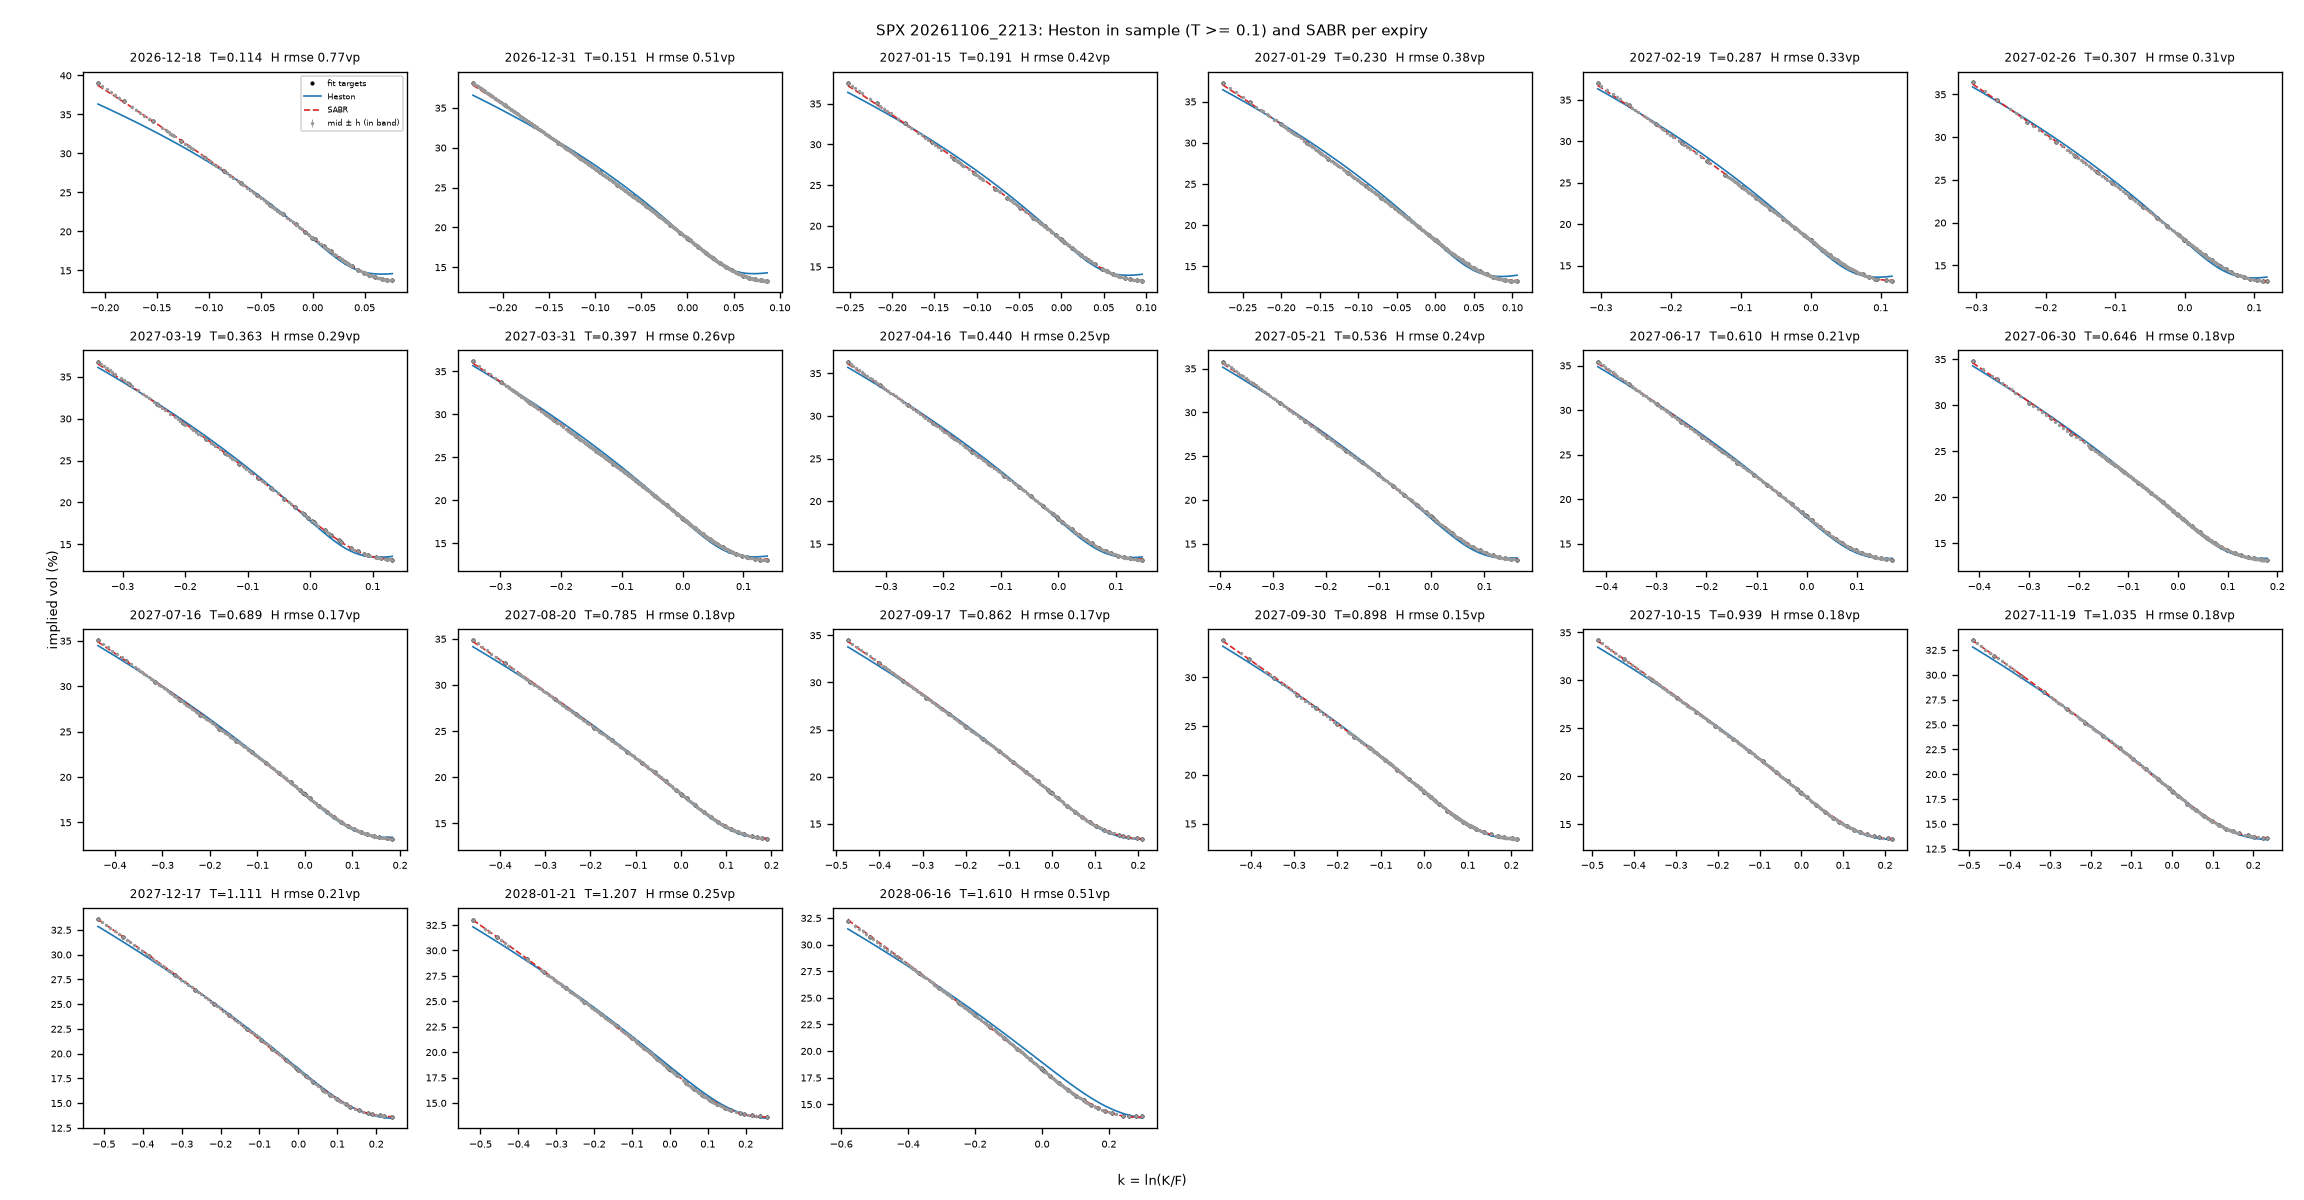
\includegraphics[width=\textwidth]{calibration_smiles_long_20261106_2213.png}
\caption{The 21 in-sample expiries. Grey dots: mids within the band with $\pm h$ bars; black dots: thinned targets;
blue line: Heston; red dashes: SABR for that expiry. The Heston RMSE is in the title.}
\label{fig:cal-long}

\bigskip
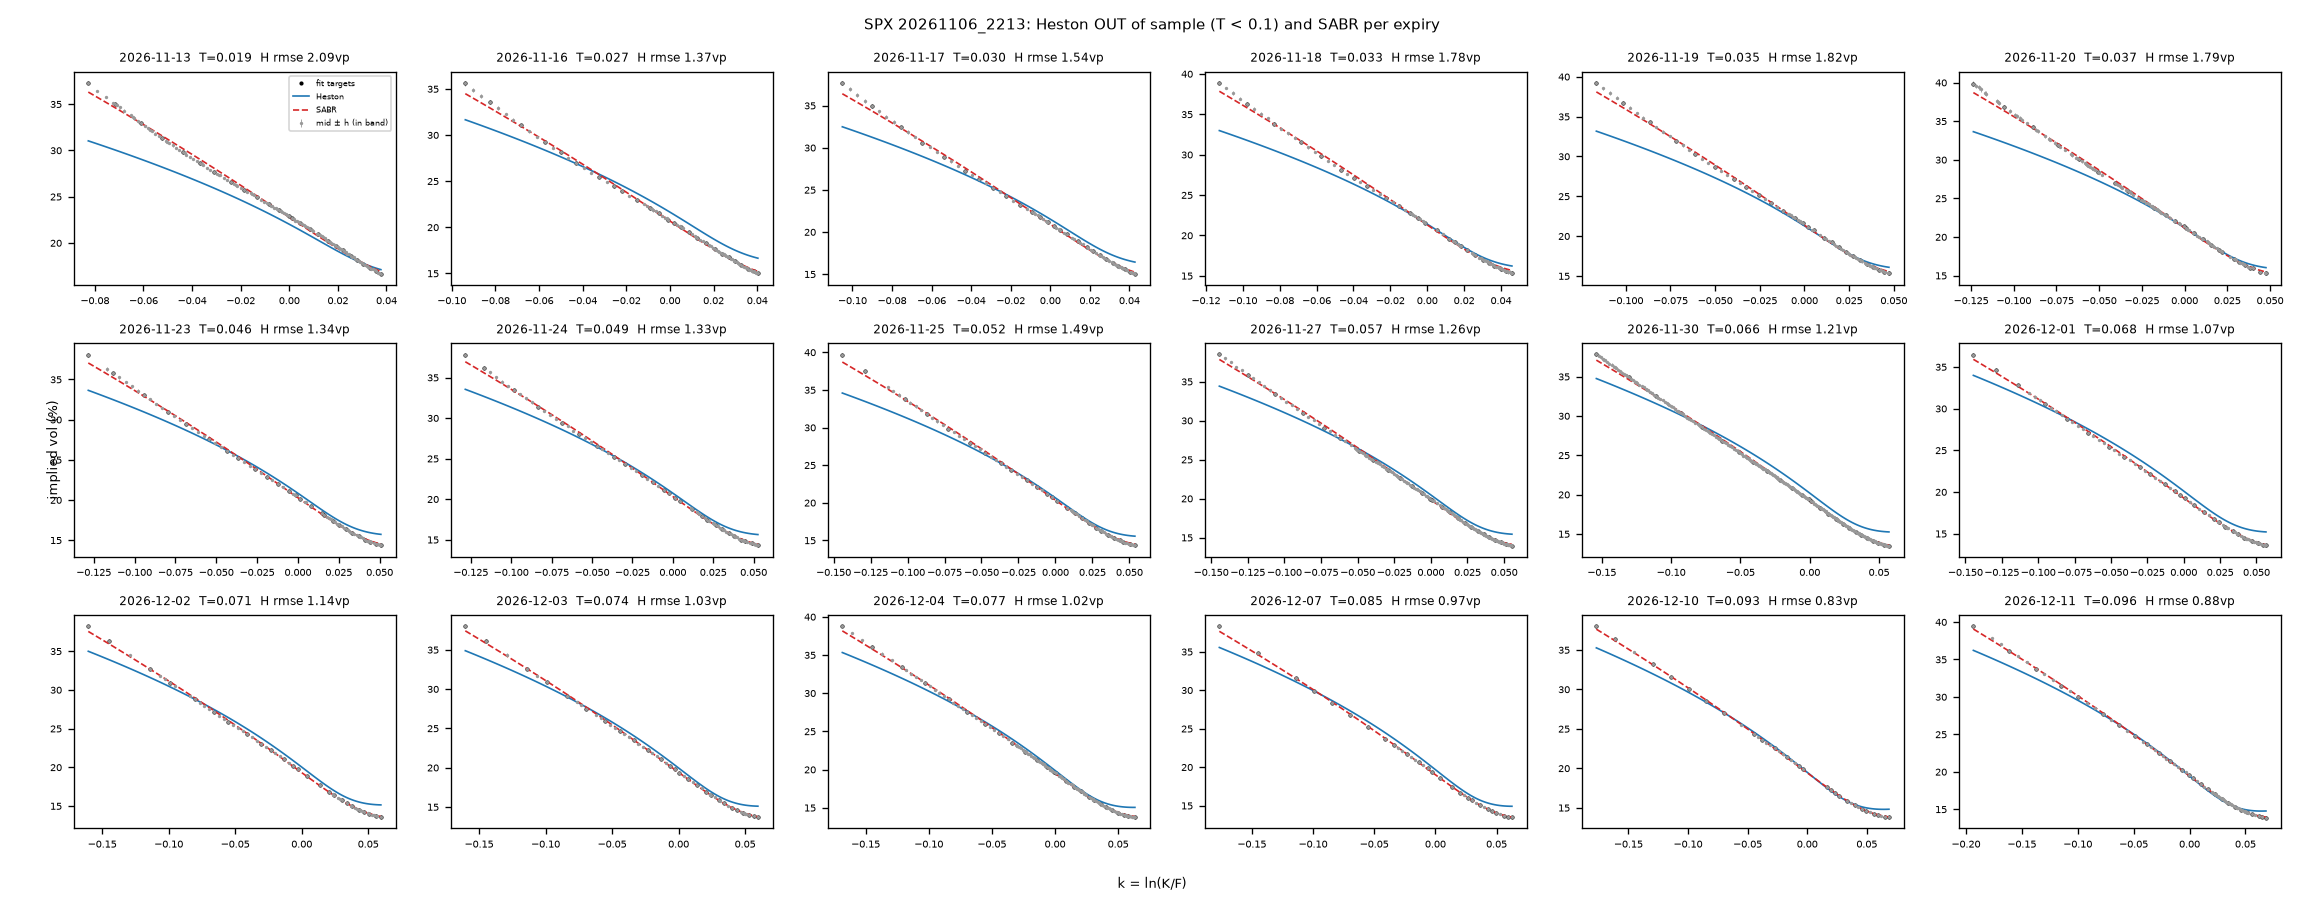
\includegraphics[width=\textwidth]{calibration_smiles_short_20261106_2213.png}
\caption{The 18 out-of-sample expiries ($T<0.1$), same legend: Heston is too flat on every weekly.}
\label{fig:cal-short}
\end{figure}

Table~\ref{tab:cal-rmse} summarizes the error. In Figure~\ref{fig:cal-long} Heston follows the central part well; the
in-sample error is U-shaped, 0.77 points on the first expiry ($T=0.114$), below 0.2 around one year, 0.51 on the last
($T=1.61$, where Heston also sits above the market at the money: 18.94\% against 18.29\%). A single $\kappa$ finds a
compromise. In Figure~\ref{fig:cal-short} the short-end failure is evident, as \eqref{eq:cal-g} predicts: Heston is too
low in the left wing and too high on the right. The worst expiry is 2026-11-13 ($T=0.019$): RMSE 2.09 and maximum
deviation 6.29 points. SABR sits on the data everywhere.

\subsection{Sensitivity: what the SEs do not say}
The last columns of Table~\ref{tab:cal-fit} redo the fit changing one choice at a time. With 50 targets per expiry
(1077 quotes) the parameters move by at most 1.06 SE; with the price objective function by at most 0.83 SE. With the
window $T\ge2$ weeks (33 expiries, 874 quotes), instead, $\kappa$ goes to 5.96 ($+12.97$ SE) and $\xi$ to 1.96
($+12.90$ SE): the short expiries ask for faster mean reversion and more vol-of-vol.

\begin{idea}[title={Key idea: estimation error versus model error}]
Curvature SEs say how narrow the minimum is \emph{if the model is right}. But $s^2=7.37$ says it is not, and the window
alone moves $\kappa$ and $\xi$ by about 13 SE: the true uncertainty is about \textbf{ten times} that of the SEs. It
should be reported as the range of the variants: $\kappa\in[4.49,5.96]$ against SE 0.107, $\xi\in[1.62,1.96]$ against
SE 0.024. ``$\kappa=4.58\pm0.11$'' would be misleading.
\end{idea}

\section{SABR expiry by expiry}
\subsection{\texorpdfstring{The fit and the cap on $\alpha$}{The fit and the cap on alpha}}
For each expiry $(\alpha,\rho,\nu)$ is calibrated with $\beta=1$, with the same residual \eqref{eq:cal-res} and the
Hagan volatility \eqref{eq:hagan} in place of the Heston one: no COS, no inversion. There are 5 starts: a seed from
the parabola \eqref{eq:sabr-taylor} fitted near the money, plus 4 Sobol points in $\rho$ and $\ln\nu$, with $\alpha$
derived from the ATM volatility.

Deriving $\alpha$ from the ATM volatility requires \eqref{eq:alpha-atm}, which for $\rho<0$ has no positive roots above
the cap \eqref{eq:tetto}. The project chooses a \emph{restriction}, not a penalty.
\begin{itemize}
\item The objective function uses $(\alpha,\rho,\nu)$ directly: \eqref{eq:alpha-atm} does not appear in it, and the cap
creates no holes in the function.
\item \eqref{eq:alpha-atm} is used only for the starts; a start without a positive root is discarded and counted.
\item Where Hagan gives \code{NaN} ($1+c_1T\le0$), TRF rejects the trial point by shrinking the trust region.
\end{itemize}

\begin{progetto}[title={In the qpricer project: SABR on the 39 expiries}]
39 fits out of 39, 0 starts discarded out of 195, no parameter at the boundary. RMSE from 0.057 to 0.307 vol points;
$\rho$ between $-0.81$ and $-0.74$. An independent check, with 9 starts of its own and without \eqref{eq:alpha-atm},
recovers the same parameters to $10^{-6}$: the restriction did not distort the fit. The SABR smiles have no calendar
or butterfly violations.
\end{progetto}

\begin{table}[htbp]
\centering
\small
\caption{SABR ($\beta=1$) on four representative expiries. RMSE in vol points.}
\label{tab:cal-sabr}
\begin{tabularx}{\textwidth}{X r r r r r r}
\toprule
expiry & $T$ & $\alpha$ & $\rho$ & $\nu$ & $\nu^2T$ & RMSE\\
\midrule
2026-11-13 & 0.019 & 0.2285 & $-0.809$ & 4.297 & 0.352 & 0.299\\
2026-12-18 & 0.114 & 0.1930 & $-0.780$ & 2.667 & 0.812 & 0.066\\
2027-05-21 & 0.536 & 0.1833 & $-0.762$ & 1.267 & 0.861 & 0.070\\
2028-06-16 & 1.610 & 0.1877 & $-0.737$ & 0.694 & 0.776 & 0.062\\
\bottomrule
\end{tabularx}
\end{table}

\subsection{\texorpdfstring{Why $\nu$ falls, and what it implies}{Why nu falls, and what it implies}}
In Table~\ref{tab:cal-sabr} $\nu$ falls from 4.30 to 0.69 while $\rho$ stays almost still. By \eqref{eq:sabr-taylor}
the SABR ATM skew is about $\tfrac12\rho\nu(1+c_1T)$ and, at fixed parameters, does not decay with $T$: SABR has no
mean reversion, and to follow the market skew the fit must lower $\nu$.

But $\nu^2T$ stays between 0.35 and 0.89 on \textbf{all} 39 expiries, above 0.16, the domain in which Chapter~\ref{cap:sabr} validated Hagan against Monte Carlo. Already at $\nu=1$ the gap was $+0.40$ vol points at $T=0.5$ and
$+0.82$ at $T=1$, at $k=-0.2$.

\begin{attenzione}[title={A parametrization, not a dynamics}]
The SABR fits are excellent \emph{interpolations} of each expiry's smile. But their parameters are not those of a SABR
dynamics that reprices those vanillas: a SABR Monte Carlo with the same $(\alpha,\rho,\nu)$ would give different
smiles. They should be read as parametrizations through the Hagan formula. And per-expiry SABR says nothing about how
the smiles connect over time: it cannot be used to price a path-dependent product.
\end{attenzione}

\paragraph{SABR on Heston smiles.} Fitting SABR to the smiles generated by Heston (set S1) on the same grid, the RMSE
grows with expiry: from 0.010 points at $T=0.019$ to 0.123 at $T=1.61$ (maximum 0.184; Spearman correlation 0.90). As
$T$ grows, Heston's mean reversion shapes the smile in a way SABR does not reproduce.

\section{No-arbitrage checks}
The filter of Chapter~\ref{cap:dati} guarantees monotonicity and vertical spreads. Here calendar and convexity are
checked as a \emph{diagnostic}.

\subsection{Calendar}
\noindent\textbf{Step 1.} With proportional dividends $X_t=S_t/F(0,t)$ is a martingale with $X_0=1$, and the
normalized undiscounted call with expiry $T$ and log-moneyness $k=\ln(K/F_T)$ is worth $\E(X_T-e^k)^+$.

\noindent\textbf{Step 2.} $x\mapsto(x-e^k)^+$ is convex; for $T_1<T_2$, conditioning on $\mathcal F_{T_1}$ and using
Jensen, $\E(X_{T_2}-e^k)^+\ge\E(X_{T_1}-e^k)^+$.

\noindent\textbf{Step 3.} The normalized call is Black as a function of $k$ and of the \textbf{total variance}
$w=\sigma^2T$, and it is increasing in $w$. Hence
\begin{equation}\label{eq:cal-calendario}
w(k,T_2)\ge w(k,T_1)\qquad\text{for } T_2>T_1,\ k\text{ fixed}.
\end{equation}
The condition is on the total variance, not on the volatility, which can fall with $T$.

For each of the 38 pairs of consecutive expiries, $w$ is interpolated linearly in $k$ between the quotes of each
expiry, only on the common interval (extrapolating would invent violations). Violation \emph{on the mid}:
$w^m_{j+1}(k)<w^m_j(k)$; \emph{strict}: $w^a_{j+1}(k)<w^b_j(k)$.

\subsection{Butterfly}
\noindent\textbf{Step 1.} For three consecutive strikes let
\[
\lambda_i=\frac{K_{i+1}-K_i}{K_{i+1}-K_{i-1}},\qquad\text{so that}\qquad K_i=\lambda_iK_{i-1}+(1-\lambda_i)K_{i+1}.
\]

\noindent\textbf{Step 2.} The ``tent'' portfolio (long $\lambda_i$ calls at $K_{i-1}$, long $1-\lambda_i$ at
$K_{i+1}$, short one at $K_i$) has payoff $\ge0$, because $K\mapsto(x-K)^+$ is convex. Hence its price is
non-negative:
\begin{equation}\label{eq:cal-butterfly}
B_i=\lambda_ic_{i-1}+(1-\lambda_i)c_{i+1}-c_i\ge0 .
\end{equation}
\noindent\textbf{Step 3.} In the limit of dense strikes this is $\partial^2C/\partial K^2\ge0$: by
Breeden--Litzenberger \eqref{eq:breeden}, a non-negative density.

The undiscounted calls are built by parity, $c_i=V_i/\DF+(F-K_i)^+$; parity adds a function linear in $K$ that
vanishes from $B_i$, except in the triples straddling $F$. Violation \emph{on the mid}: $B^m_i<0$; \emph{strict}:
\[
\lambda_ic^a_{i-1}+(1-\lambda_i)c^a_{i+1}-c^b_i<0,
\]
that is, buying the wings at the ask and selling the body at the bid would give a credit. Size: $z_i=-B^m_i/h^B_i$,
with $h^B_i$ the half-spread of the butterfly.

\begin{progetto}[title={In the qpricer project: the SPX surface}]
\begin{itemize}
\item \textbf{Calendar}: 11{,}054 points, 0 violations on the mid, 0 strict.
\item \textbf{Butterfly}: 7547 triples, \textbf{2126 violations on the mid}, \textbf{0 strict}, maximum $z$ 0.43:
every shortfall on the mid is less than half the butterfly half-spread, hence inside the spreads.
\end{itemize}
The checks have power: a flat surface gives 0 violations, a mid raised by 3 half-spreads and two swapped smiles are
flagged, the Heston S1 surface has no strict violations.
\end{progetto}

\begin{attenzione}
With strikes 5 points apart the butterfly is tiny and its mid is quoting noise. The correct statement is: ``no
calendar or convexity arbitrage is tradable at bid/ask prices''.
\end{attenzione}

\section{The link with the autocallable}
The file \code{data/processed/heston\_fit\_20261106\_2213.json} contains $\hat p$ with SEs and provenance, and Chapter~\ref{cap:autocallable} uses it to price the autocallables. The window $T\ge0.1$ covers the dates of \mbox{AC-Q} (up to
1.5 years), while \mbox{AC-A} (3 years) is an extrapolation beyond the last quoted expiry. On \mbox{AC-Q} Heston is
worth 1.87\% of notional less than Black ($-0.018688$, CRN SE 0.000217) and the par coupon rises from 5.60\% to
8.93\%; the dominant term is the skew at the 60--70\% barriers, the part of the smile that the calibration fits. Two
caveats: Black is evaluated at the ATM volatility of calibrated Heston (18.85\%), not at the market one (18.29\%); and
the window uncertainty ($\kappa$ and $\xi$ moved by about 13 SE) has not been propagated to the autocallable price.

\needspace{6\baselineskip}
\begin{riassunto}
\begin{itemize}
\item Targets: OTM volatilities in the 5$\Delta$ band, thinned to 25--27 per expiry; volatility residuals weighted by
$1/\max(h,0.001)$, equivalent at first order to prices weighted by $1/\vega^2$.
\item Heston on $T\ge0.1$, the rest out of sample: Heston has a single clock, $1/\kappa$.
\item COS frozen at $(16384,64)$ with an a-priori budget of $10^{-5}$ in market vega (measured $9.21\times10^{-6}$),
which is not a volatility accuracy. Narrowed box; on the original box 20 starts out of 20 find the same optimum.
\item Synthetic test S1, S2: tolerances from the sandwich before the fit, G1--G4 passed; expected false alarms about 8\%.
\item SPX: $\hat p=(0.052372,\,4.5751,\,0.052925,\,1.6477,\,-0.75180)$, $\nu_F=0.178$. RMSE 0.328 vol points in sample,
1.379 out of sample. The SEs underestimate the uncertainty by a factor of about ten.
\item SABR: RMSE 0.057--0.307, but $\nu^2T$ between 0.35 and 0.89: parametrizations, not dynamics.
\item No tradable arbitrage; 2126 negative butterflies on the mid, all inside the spreads.
\end{itemize}
\end{riassunto}

\needspace{6\baselineskip}
\begin{domande}
\begin{enumerate}
\item In what sense do volatility residuals and prices divided by vega coincide at first order? Why are volatilities
preferred?
\item Why does a COS that chooses $(N,L)$ by itself ruin a finite-difference Jacobian?
\item How do you show that narrowing the constraints did not change the result?
\item What is the $\kappa$--$\theta$ ridge, and why does it not show up on this window?
\item Why can Heston not fit weeklies and long expiries together? \emph{Hint:} \eqref{eq:cal-g}.
\item The SEs say $\kappa=4.58\pm0.11$: what do you report instead?
\item Why does the SABR $\nu$ fall with $T$, and what does $\nu^2T>0.16$ imply?
\item Derive the calendar and butterfly conditions. What is the difference between a violation on the mid and a strict
one?
\end{enumerate}
\end{domande}

\chapter{Monte Carlo versus closed forms: the benchmark}
\label{cap:benchmark}

In Chapter~\ref{cap:mc} we saw how a Monte Carlo (MC) price is estimated, how its error is measured and how Heston is
simulated. Here we put all of this to the test on cases in which the exact price is known. There are four questions:
\begin{itemize}
\item does the error really fall as $N^{-1/2}$, and how do we check it without fooling ourselves?
\item how much do the variance-reduction techniques (antithetic variates, control variate, quasi-Monte Carlo) gain,
for the same number of scenarios and for the same computing time?
\item how large is the discretization bias of the QE-M scheme at the step used in the project?
\item how do we show that the figures and tables were really produced by the declared code?
\end{itemize}
A single rule runs through the whole chapter: the measurement procedure is fixed \emph{before} looking at the
results, and it is not changed afterwards.

\section{The experimental design}
\subsection{The test cases}
We use three parameter sets (``sets'') and, for each, two contracts: an at-the-money call ($K=F$) and a 90\% put
($K=0.9\,F$). The two strikes of a set are priced on the same paths.

\textbf{The market point.} To tie the benchmark to the data, $F$, $\DF$ and $T$ come from the parity table of Chapter~\ref{cap:dati}: the expiry \mbox{2027-11-19}, the kept expiry closest to one year, with
\[
T=1.034734,\qquad F=7677.961695,\qquad \DF=0.951346 .
\]
Two sets are defined on this point.
\begin{itemize}
\item \textbf{bsm}: Black with constant volatility $\sigma=18.40\%$. It is not a hand-picked number: it is the
at-the-money implied volatility of calibrated Heston at that expiry (COS price at $K=F$, then inverted). The path is
sampled \emph{exactly} in a single step,
\[
\ln\frac{F_T}F=-\tfrac12\sigma^2T+\sigma\sqrt T\,Z,\qquad Z\sim\N(0,1),
\]
so the MC error is noise \emph{only}: there is no discretization bias. Reference: Black-76.
\item \textbf{heston\_cal}: Heston with the calibrated parameters of Chapter~\ref{cap:calibrazione}
($\kappa=4.575$, $\theta=0.0529$, $\xi=1.648$, $\rho=-0.752$, $v_0=0.0524$; Feller violated). QE-M simulation
(Section~\ref{sec:qe-m}) on a uniform grid of $\lceil32T\rceil=34$ steps, that is $\Delta t\le1/32$.
\end{itemize}
The third set is an external anchor:
\begin{itemize}
\item \textbf{heston\_fo}: the Fang and Oosterlee set ($\kappa=1.5768$, $\theta=0.0398$, $\xi=0.5751$,
$\rho=-0.5711$, $v_0=0.0175$) with $F=100$, $\DF=1$, $T=1$ and 32 QE-M steps.
\end{itemize}

\begin{esempio}[title={Example: same ATM vol, very different puts}]
The reference prices are:
\begin{center}
\small
\begin{tabular}{lrr}
\toprule
set & ATM call & 90\% put\\
\midrule
bsm & 544.7286 & 231.8087\\
heston\_cal & 544.7286 & 317.2988\\
heston\_fo & 5.785155 & 2.709532\\
\bottomrule
\end{tabular}
\end{center}
The at-the-money call is identical in the first two sets \emph{by construction}: the $\sigma$ of bsm is precisely the
Heston ATM implied vol. The 90\% put, instead, costs about 37\% more under Heston. This is the skew: with
$\rho=-0.75$ the Heston implied vol at that strike is 21.89\%, against Black's flat 18.40\%. The benchmark therefore
covers both a ``smooth'' case and a case in which the left tail weighs heavily.
\end{esempio}

\subsection{The reference: why COS is ``exact enough''}
Under Heston the reference is the COS method (Chapter~\ref{cap:heston}). But a test ``MC within 3 SE of the
reference'' makes sense only if the error of the reference is \emph{negligible} compared with the SE. Otherwise the
test measures the error of the reference, not that of the MC.

The criterion, fixed in advance, is
\begin{equation}\label{eq:bm-rif}
\max|\text{COS}-\text{Lewis}|\ \le\ 0.01\times\min\SE ,
\end{equation}
where the minimum is taken over all Monte Carlo SEs of the benchmark. The smallest Heston SE is
$3.09\times10^{-3}$, so the threshold is $3.09\times10^{-5}$.

Why three independent methods give confidence:
\begin{itemize}
\item \textbf{COS} expands the density in a cosine series on a truncated interval $[a,b]$; its errors are series and
truncation errors.
\item \textbf{Lewis} integrates the characteristic function along another contour with adaptive quadrature: no
interval, no series.
\item \textbf{Gil-Pelaez} (written by an independent check, with its own code) inverts the two probabilities $P_1$,
$P_2$ separately with an integral over $[0,\infty)$.
\end{itemize}
The numerical errors of the three methods have nothing in common. If they agree, the only thing they share is the
characteristic function, which is in turn checked against published values.

\begin{progetto}[title={In the qpricer project: accuracy of the references}]
\begin{itemize}
\item COS against Lewis: $7.36\times10^{-9}$ at most (heston\_cal, $F=7678$: a relative error of about $10^{-12}$),
$1.9\times10^{-10}$ on the FO set. Threshold $3.09\times10^{-5}$: met with four orders of magnitude to spare.
\item Independent Gil-Pelaez: differs from COS by $7.36\times10^{-9}$ and $1.9\times10^{-10}$, and from Lewis by about
$10^{-12}$.
\item FO set, ATM call: COS $5.785155434$ against the published value $5.785155450$, a gap of $-1.6\times10^{-8}$.
\end{itemize}
The six reference prices are frozen in \path{tests/golden/phase6_benchmark_refs.json}, written by the independent
check with its own Gil-Pelaez.
\end{progetto}

\subsection{Grid, replications and seeds}
\begin{itemize}
\item \textbf{Grid.} $N=2^{10},2^{11},\dots,2^{20}$: 11 points from 1024 to 1{,}048{,}576. Powers of 2 are needed for
Sobol' (Section~\ref{sec:bm-rqmc}).
\item \textbf{Honest counting.} $N$ is always the total number of terminal samples, for \emph{every} method: for
antithetics $N/2$ pairs, for Sobol' 16 nets of $N/16$ points. Only in this way is the comparison ``at equal $N$''
fair.
\item \textbf{Replications.} $R=16$ independent replications for each (set, method, $N$). Replication $r=0$ is the
``single run''.
\item \textbf{Seeds.} The seed of replication $r$ is a fixed formula,
\[
\text{seed}=20261110+10^6\cdot\text{set}+10^5\cdot\text{method}+10^3\cdot i_N+r ,
\]
with set and method numbered in a fixed order. No seed can be chosen after the fact.
\item \textbf{Parallelism.} Each task has its own integer seed, so the results do not depend on the number of
processes used.
\end{itemize}

\section{\texorpdfstring{The $N^{-1/2}$ law}{The N\textasciicircum(-1/2) law}}
\label{sec:bm-pendenza}
\subsection{What is measured: noise and bias kept apart}
The gate of this phase requires the log-log slope of the plain MC error to lie in $[-0.6,-0.4]$. The procedure,
declared before running the full benchmark, is:
\begin{enumerate}
\item OLS regression of $\ln y$ on $\ln N$ over \emph{all} 11 points (no point excluded);
\item $y$ is an \textbf{error metric over the $R=16$ replications}:
\begin{itemize}
\item for bsm, the RMSE against Black: $\mathrm{RMSE}=\sqrt{\tfrac1R\sum_r(\hat V_r-V)^2}$;
\item for Heston, the standard deviation of the replications around their mean (noise only).
\end{itemize}
\end{enumerate}

\begin{perche}[title={Why the bias is removed from the metric for Heston}]
With fixed-step QE-M the expected price is $V+b(\Delta t)$, with $b$ constant in $N$. The RMSE against COS is then
\[
\mathrm{RMSE}(N)\approx\sqrt{b^2+\sigma_g^2/N}\ \xrightarrow{N\to\infty}\ |b| :
\]
for large $N$ the curve flattens onto the bias and the slope tends to zero. The gate would fail for a reason that has
nothing to do with the $N^{-1/2}$ law. The standard deviation of the replications, on the other hand, does not see a
constant added to all prices: it measures only the noise. The bias is measured separately (Section~\ref{sec:bm-bias}).

An independent check verified both things: adding a constant to every price leaves the metric unchanged (identical to
$10^{-9}$), and even when the bias is included (RMSE against its own Gil-Pelaez) the four Heston slopes stay within
the band ($-0.516$, $-0.537$, $-0.520$, $-0.540$), because at the benchmark step the bias is smaller than the SE even
at $N=2^{20}$.
\end{perche}

\subsection{How precise the estimated slope is}
With $R=16$ replications, the RMSE at a given $N$ has a relative error of about $1/\sqrt{2R}\approx18\%$, that is a
noise of about $0.18$ on $\ln y$. The OLS slope has variance $\sigma^2/\sum_j(x_j-\bar x)^2$, with $x_j=\ln N_j$.
The points are equally spaced by $\ln2$ and there are 11 of them, hence
\[
\sum_j(x_j-\bar x)^2=(\ln2)^2\sum_{k=-5}^{5}k^2=110\,(\ln2)^2\approx52.9,
\qquad
\mathrm{sd}(\text{slope})\approx\frac{0.18}{\sqrt{52.9}}\approx0.025 .
\]
The band $[-0.6,-0.4]$ is therefore about 4 standard deviations wide on each side of $-0.5$: correct code misses it
with negligible probability, and a bug that really changes the order of convergence misses it almost always.

\subsection{Why the error of a single run is not fitted}
It is tempting to plot $|\hat V-V|$ of a single run against $N$ and fit the line. It is a bad idea. For one run,
$\hat V-V\approx\SE\cdot Z$ with $Z\sim\N(0,1)$, hence
\[
\ln|\hat V-V|\approx\ln\SE+\ln|Z| .
\]
The term $\ln|Z|$ has variance $\pi^2/8\approx1.23$, that is standard deviation $\approx1.1$: noise of order 1 on
\emph{every} point. Redoing the computation above, the standard deviation of the slope would be about
$1.1/\sqrt{52.9}\approx0.15$, wider than the whole half-band of the gate. The slope of a single run can fall outside
the band with perfect code, or inside it with wrong code. This is why the single-run error is shown in the plots (the
crosses), but never fitted.

\subsection{Why the slope of the SE proves nothing}
The other temptation is to fit the SE estimated by the run: $\SE=s_g/\sqrt N$. But
\[
\ln\SE=\ln s_g-\tfrac12\ln N ,
\]
and $s_g$ converges to $\sigma_g$ with a relative error of order $1/\sqrt{2N}$, which is tiny. The slope is therefore
$-0.5$ \emph{by construction}, for any code that computes a sample standard deviation and divides it by $\sqrt N$.
Even a wrong SE has slope $-0.5$: for example an antithetic SE computed on the $N$ correlated payoffs instead of on the
$N/2$ pair means.

\begin{attenzione}[title={A gate that cannot fail is not evidence}]
In the project the gate fits both quantities, for a total of 12 rows. An independent check pointed out that the 6 SE
rows cannot fail, so the count ``52 gates out of 52'' overstates the evidence. The SE rows remain as a consistency
check; the real evidence comes from:
\begin{itemize}
\item the 6 slopes of the error metric over the replications;
\item 104 slopes recomputed by an independent check with fresh seeds;
\item the \textbf{SE honesty ratio}, $\sqrt{\overline{\text{err}^2}/\overline{\SE^2}}$, which is about 1 only if the
declared SE really is the standard deviation of the error.
\end{itemize}
\end{attenzione}

\subsection{The measured slopes}
\begin{table}[ht]
\centering
\small
\caption{Log-log slopes of plain MC over $N=2^{10}\dots2^{20}$. ``SE'': fit of the SE of run $r=0$ (consistency
check); ``metric'': fit of the error metric over the 16 replications (RMSE for bsm, standard deviation of the
replications for Heston), with the OLS standard deviation.}
\label{tab:bm-pendenze}
\begin{tabular*}{\textwidth}{@{\extracolsep{\fill}}l r r r r@{}}
\toprule
& & & \multicolumn{2}{c}{fresh seeds}\\
\cmidrule(l){4-5}
set and contract & SE & metric & mean $\pm$ sd & trials\\
\midrule
bsm, ATM call & $-0.501$ & $-0.538\pm0.021$ & $-0.509\pm0.023$ & 40\\
bsm, 90\% put & $-0.503$ & $-0.487\pm0.025$ & $-0.503\pm0.029$ & 40\\
heston\_cal, ATM call & $-0.499$ & $-0.517\pm0.022$ & $-0.487\pm0.014$ & 6\\
heston\_cal, 90\% put & $-0.499$ & $-0.554\pm0.020$ & $-0.479\pm0.018$ & 6\\
heston\_fo, ATM call & $-0.505$ & $-0.518\pm0.033$ & $-0.484\pm0.032$ & 6\\
heston\_fo, 90\% put & $-0.500$ & $-0.541\pm0.032$ & $-0.489\pm0.022$ & 6\\
\bottomrule
\end{tabular*}
\end{table}

Table~\ref{tab:bm-pendenze} summarizes the result.
\begin{itemize}
\item The 6 slopes of the error metric range from $-0.554$ to $-0.487$, with OLS standard deviations between 0.020
and 0.033: all within the band, and all compatible with $-0.5$ within about 2.7 standard deviations.
\item An independent check repeated the \emph{same} procedure with fresh seeds, declared in advance: 40 trials for
each bsm strike and 6 for each strike of the two Heston sets, for a total of \textbf{104 slopes}. They range from
$-0.558$ to $-0.445$: none outside the band.
\item The Heston slopes of the project run are all slightly below $-0.5$, those of the check all slightly above. The
difference is about 1.8 standard deviations of a mean over 6 trials, and the check's trials on the two sets share
seeds, so they are correlated: it is not significant.
\end{itemize}

\begin{figure}[p]
\centering
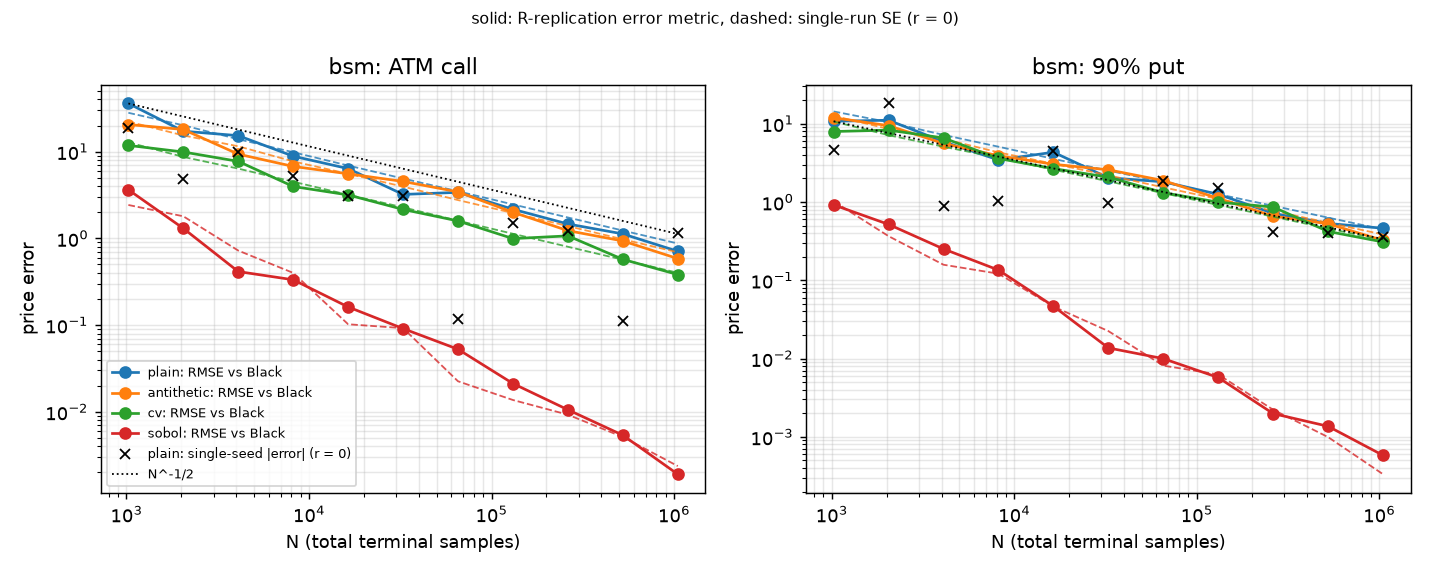
\includegraphics[width=\textwidth]{benchmark_convergence_bsm.png}
\caption{Set bsm: error against $N$ on a log-log scale. Solid lines: RMSE over the 16 replications for each method;
dashed: SE of the single run; crosses: $|\hat V-V|$ of the single plain-MC run; dotted: $N^{-1/2}$ guide.}
\label{fig:bm-conv-bsm}

\bigskip
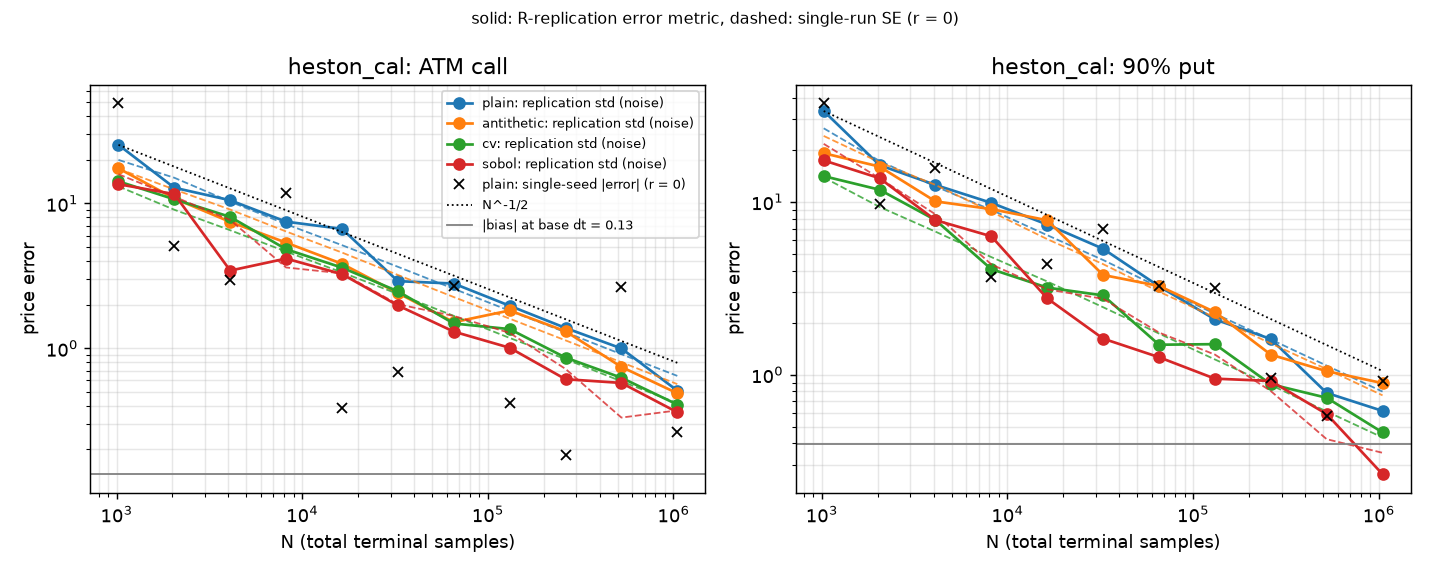
\includegraphics[width=\textwidth]{benchmark_convergence_heston_cal.png}
\caption{Set heston\_cal: as above, but the metric is the standard deviation of the replications (noise only). The
horizontal grey line is the absolute value of the QE-M bias at the benchmark step.}
\label{fig:bm-conv-cal}

\bigskip
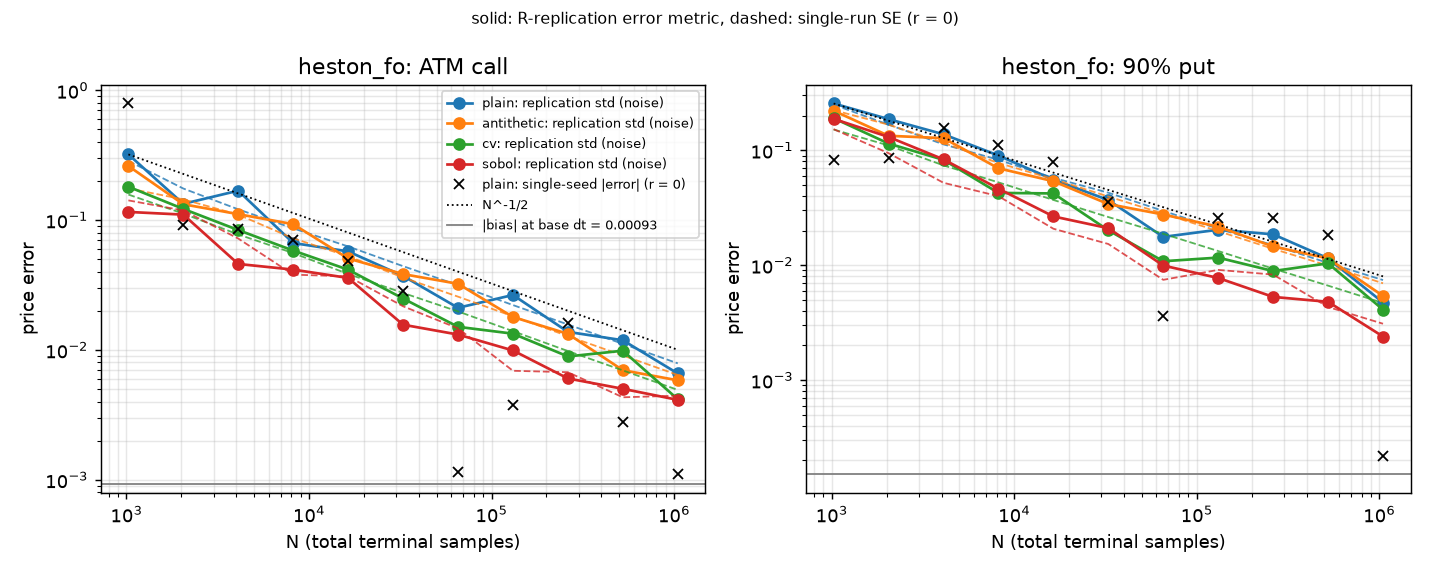
\includegraphics[width=\textwidth]{benchmark_convergence_heston_fo.png}
\caption{Set heston\_fo (Fang--Oosterlee): same legend as Figure~\ref{fig:bm-conv-cal}.}
\label{fig:bm-conv-fo}
\end{figure}

Figures~\ref{fig:bm-conv-bsm}, \ref{fig:bm-conv-cal} and~\ref{fig:bm-conv-fo} show the full curves. Three things to
note.
\begin{itemize}
\item The solid lines of plain, antithetic and control variate are parallel lines of slope $-\tfrac12$: variance
reduction shifts the line down, it does not change its slope.
\item The crosses (error of one run) jump by an order of magnitude from one point to the next: this is the
$\ln|Z|$ noise seen above.
\item Sobol' on bsm (red, Figure~\ref{fig:bm-conv-bsm}) has a clearly steeper slope: it is the only case in which the
method changes the \emph{order} of convergence (Section~\ref{sec:bm-rqmc}).
\end{itemize}

\subsection{The other statistical checks}
\begin{itemize}
\item \textbf{Plain MC within 3 SE at every $N$.} 6 (set, strike) pairs times 11 values of $N$: 66 comparisons, on
run $r=0$. With correct code, by \eqref{eq:test-multipli}, the probability of at least one false alarm is
$1-0.9973^{66}\approx16\%$. The number was written down \emph{in advance}, so that any excursion between 3 and 3.5 SE
would be read as expected multiplicity and not ``fixed'' by changing the seed. Result: $\max|z|=2.90$, none beyond 3.
\item \textbf{Unbiased estimators.} For antithetics, control variate and Sobol' all the $R\times11$ runs are pooled
with weights proportional to $N$:
\[
\bar V=\frac{\sum N\,\hat V}{\sum N},\qquad\SE(\bar V)=\frac{\sqrt{\sum N^2\SE^2}}{\sum N}.
\]
For bsm the comparison is with Black. For Heston it is with plain MC pooled at the same step, with
$\sqrt{\SE_1^2+\SE_2^2}$ in the denominator: this isolates the estimator from the scheme bias, which is the same for
all. 20 comparisons, $\max|z|=2.01$.
\end{itemize}

\section{Variance reduction}
\label{sec:bm-vr}
\subsection{How the methods are compared}
Two measures, both at $N=2^{20}$:
\begin{equation}\label{eq:bm-vr-eff}
\mathrm{VR}_m=\Big(\frac{\overline{\SE}_{\text{plain}}}{\overline{\SE}_m}\Big)^2,
\qquad
\mathrm{eff}_m=\mathrm{VR}_m\times\frac{t_{\text{plain}}}{t_m},
\end{equation}
where $\overline{\SE}$ is the root mean square of the SEs over the replications and $t$ the computing time.
\begin{itemize}
\item $\mathrm{VR}$ says by how much the variance is reduced \emph{for the same number of scenarios}: for the same
error, $\mathrm{VR}$ times fewer scenarios are needed.
\item $\mathrm{eff}$, the work-normalized efficiency, says by how much the variance is reduced \emph{for the same time}. It is the measure that matters
in practice: a method that halves the variance but doubles the time is useless ($\mathrm{eff}=1$).
\end{itemize}
VR could also be defined as the ratio of the replication error metrics. But at a single $N$ that estimate rests on 16
replications: the ratio of two variances with 15 degrees of freedom has a relative error of about $\pm50$--70\%. This
is why the SE-based VR is reported.

\subsection{Antithetic variates}
\textbf{The idea.} If $Z\sim\N(0,1)$, so is $-Z$. One uses $N/2$ normals $Z_j$ and their negatives, and averages the
payoff over the pairs:
\[
h_j=\tfrac12\big[g(Z_j)+g(-Z_j)\big],\qquad\hat V=\DF\,\frac2N\sum_{j=1}^{N/2}h_j .
\]
Under Heston both rows of normals $(Z_v,Z_\perp)$ of each step have their sign flipped.

\textbf{Step 1: the variance.} The $h_j$ are mutually independent, and
\[
\Var h=\tfrac14\big[2\Var g+2\Cov(g(Z),g(-Z))\big]=\tfrac12\Var g\,(1+\rho_A),
\qquad\rho_A=\Corr\big(g(Z),g(-Z)\big).
\]
With $N/2$ pairs, $\Var\hat V=\DF^2\,\Var g\,(1+\rho_A)/N$, hence
\[
\mathrm{VR}=\frac1{1+\rho_A}.
\]
There is a gain only if $\rho_A<0$. If the payoff is even ($\rho_A=+1$, for example a straddle under Black)
antithetics \emph{double} the variance.

\textbf{Step 2: even part and odd part.} Every function can be written as the sum of an odd part and an even part:
\[
g(z)=\underbrace{\tfrac12[g(z)-g(-z)]}_{g_o}+\underbrace{\tfrac12[g(z)+g(-z)]}_{g_e}.
\]
The pair mean is exactly $h=g_e(Z)$: antithetics \emph{cancel the odd part} and leave the even part intact. Since
$g_o$ and $g_e$ are uncorrelated (their product is odd, hence has zero mean),
\[
\mathrm{VR}=\frac{\Var g}{\Var g_e}=1+\frac{\Var g_o}{\Var g_e}.
\]

\begin{perche}[title={Why antithetics help little on convex payoffs}]
For a payoff linear in $Z$ the even part is constant and VR is infinite. An at-the-money call is, to a first
approximation, $\max(z,0)=\tfrac12z+\tfrac12|z|$: half linear (odd, removed) and half ``absolute value'' (even,
surviving). Convexity is precisely the even part, and antithetics do not touch it. For an OTM put the payoff is almost
always zero and the even part weighs even more. The numbers confirm it: under Black VR is 1.59 (ATM call) and 1.35
(90\% put), against the exact values 1.594 and 1.347 computed by an independent check with Gauss--Hermite quadrature.
\end{perche}

\begin{attenzione}[title={Honest counting of the pairs}]
The SE is computed from the $N/2$ pair means, which are independent, \emph{never} from the $N$ payoffs as if they were
independent: they are not. The ``naive'' SE on the $N$ payoffs has an error that depends on the sign of $\rho_A$; in
the project it differs from the correct value by more than 5\%. Above all, it would still have slope $-\tfrac12$: the
slope gate would not notice. In the code (\code{vr.antithetic\_estimate}) an odd $N$ raises an error.
\end{attenzione}

A small practical advantage: antithetics draw half as many normals, so they are also a little faster (under Black
0.0135 s against 0.019 s at $N=2^{20}$). This is why their efficiency exceeds their VR.

\subsection{Control variate: the terminal forward}
Chapter~\ref{cap:asiatiche} derived the control variate \eqref{eq:cv} and the factor $\mathrm{VR}=1/(1-\rho_{XY}^2)$
\eqref{eq:vr}. Here the choice is
\[
Y=\DF\,g(F_T),\qquad X=F_T,\qquad\E X=F .
\]

\textbf{Why the mean is exact.} Under Black the sampling is exact. Under Heston QE-M is used, which is an exact
discrete martingale: $\E[e^{x_{n+1}-x_n}\mid v_n]=1$ at every step (Section~\ref{sec:qe-m}), hence $\E F_T=F$ on any
grid. The control variate therefore adds no discretization bias. With plain QE this would not be so: the spurious
drift of $F_T$ would pass straight into the price. An independent check verified that with QE-M $\overline{F_T}=F$
even at the coarse step $T/9$, with $2^{20}$ paths: $z=-0.10$.

\textbf{The estimated coefficient.} $\hat\beta$ is the OLS slope of $Y$ on $X$ computed on the same paths, and this is
what introduces a small bias. It is computed in three steps. Let $x_i=X_i-F$ and let $e_i$ be the residual of the
population regression, uncorrelated with $x$.

\textit{Step 1.} At first order,
\[
\hat\beta\approx\beta+\frac{\frac1N\sum_ix_ie_i}{\Var X}.
\]

\textit{Step 2.} The estimator is $\hat V=\bar Y-\hat\beta\,\bar x$ and $\E\bar x=0$, so the bias is
\[
\E\hat V-V=-\E[\hat\beta\,\bar x]\approx-\frac{\E\big[\frac1N\sum_ix_ie_i\cdot\frac1N\sum_jx_j\big]}{\Var X}.
\]

\textit{Step 3.} The terms with $i\ne j$ have zero mean (independence and $\E x=0$); the $N$ terms with $i=j$ remain:
\begin{equation}\label{eq:bm-cv-bias}
\E\hat V-V\approx-\frac{\E[x^2e]}{N\Var X}=O\Big(\frac1N\Big).
\end{equation}
The residual is uncorrelated with $x$ but not with $x^2$ (the payoff is convex), so $\E[x^2e]\ne0$. But the bias is
$O(1/N)$, while the SE is $O(N^{-1/2})$: their ratio falls as $N^{-1/2}$.

\begin{progetto}[title={In the qpricer project: the bias of the estimated coefficient}]
Computed by an independent check with a quadrature, under Black:
\begin{itemize}
\item at $N=2^{10}$ the bias is $-0.548$ (ATM call) and $-0.400$ (put), that is 0.043 and 0.031 SE;
\item at $N=2^{20}$ it is $-5.4\times10^{-4}$, that is 0.0013 SE;
\item over 20{,}000 runs at $N=2^{10}$ the mean minus Black matches the predicted bias within 3 SE: there is no other
bias beyond the $O(1/N)$ term.
\end{itemize}
Negligible: to remove it entirely one could estimate $\beta$ on a separate pilot sample, but there is no need.
\end{progetto}

\begin{perche}[title={\texorpdfstring{Why $F_T$ beats the ``shadow Black''}{Why F\_T beats the shadow Black}}]
The alternative considered was the \emph{shadow Black}: the same payoff computed on a Black path driven by the same
normals, with a mean known in closed form (Black-76 at the expected variance). It looks ``closer'' to the payoff, but:
\begin{itemize}
\item with high vol-of-vol ($\xi=1.65$) the Heston log-returns and those of the shadow Black decorrelate, because the
Heston variance moves a lot and that of the shadow does not;
\item $F_T$ is linear and captures the ``delta'' part of \emph{any} payoff, in any model;
\item $F_T$ costs one line of code and is model-independent.
\end{itemize}
Measured on $2^{18}$ paths: VR with $F_T$ equal to 2.39 and 3.41 (heston\_cal, call and put) and 2.56 and 2.51
(heston\_fo), against 1.34, 1.75, 1.74 and 2.39 with the shadow Black. A control variate removes noise, never bias.
\end{perche}

Under Black the exact VR values with $F_T$, computed by an independent check with the partial moments of the
lognormal, are 4.726 (ATM call) and 1.885 (90\% put); the benchmark measures 4.727 and 1.885. The 90\% put is out of
the money: its payoff is zero on most paths and its correlation with $F_T$ is lower.

\subsection{Randomized quasi-Monte Carlo (Sobol')}
\label{sec:bm-rqmc}
\textbf{The idea.} An MC uses random points in $[0,1)^d$, which by chance leave holes and form clumps. A
\emph{quasi}-Monte Carlo uses deterministic \emph{low-discrepancy} points, spread much more evenly. Sobol' sequences
are ``nets'': every elementary box of volume $2^{-m}$ contains exactly the right number of points.

\textbf{Koksma--Hlawka.} For an integrand $f$ of bounded variation $V_{HK}(f)$ (in the sense of Hardy--Krause),
\begin{equation}\label{eq:bm-kh}
\Big|\frac1N\sum_{i=1}^Nf(u_i)-\int_{[0,1)^d}f\Big|\ \le\ V_{HK}(f)\,D_N^*,
\qquad D_N^*=O\Big(\frac{(\log N)^d}{N}\Big),
\end{equation}
where $D_N^*$ is the discrepancy of the points. For small $d$ the error falls almost as $N^{-1}$, much better than
$N^{-1/2}$. But the factor $(\log N)^d$ explodes with dimension, and financial payoffs, after $\Phi^{-1}$, do not have
bounded variation. \eqref{eq:bm-kh} should be taken as intuition, not as a guarantee.

\textbf{Why randomize.} A deterministic net has no standard error: one does not know how wrong one is.
\emph{Scrambling} (random permutations of the binary digits, plus a random digital shift) produces a random net that:
\begin{itemize}
\item preserves the net property (the stratification);
\item has every point, taken on its own, uniform in $[0,1)^d$, so the estimator is unbiased.
\end{itemize}
With 16 \emph{independent} scramblings of $N/16$ points each, the 16 estimates are independent and identically
distributed:
\[
\hat V=\frac1{16}\sum_{q=1}^{16}\hat V_q,\qquad\SE=\frac{s_q}{\sqrt{16}} .
\]
The child seeds are generated with \code{SeedSequence(seed).spawn(16)}. A single net has no error estimate, so no
``3 SE'' test is performed on a single run.

\begin{perche}[title={What splitting the budget into 16 nets costs}]
If the error of a net falls as $c/N$, a net of $N$ points is off by about $c/N$. Sixteen nets of $N/16$ points are
each off by about $16c/N$; the mean of 16 independent errors divides by $\sqrt{16}=4$, leaving $4c/N$. One pays a
factor $\sqrt{16}=4$ on the error, and in exchange obtains a valid SE. With an error that falls only as $N^{-1/2}$ (as
under Heston, see below) the cost disappears.
\end{perche}

\textbf{Dimensions.} Under Black a single normal is needed: $d=1$. Under Heston two normals per step are needed, hence
$d=2\times34=68$ (heston\_cal) and $d=64$ (heston\_fo). Coordinates $(2k,2k+1)$ drive step $k$, in time order, with no
Brownian bridge and no principal components.

\begin{progetto}[title={In the qpricer project: the empirical rate of Sobol'}]
Slope of the replication error metric ($\pm$ OLS standard deviation):
\begin{itemize}
\item \textbf{bsm}: $-1.015\pm0.032$ (ATM call) and $-1.089\pm0.032$ (put). In one dimension a scrambled net is a
stratified sample: for a Lipschitz payoff it would give an RMSE $\propto N^{-1.5}$. But after $\Phi^{-1}$ the payoff is
unbounded or very steep in the boundary cells ($u\to1$ for the call); those cells contribute a variance
$\propto N^{-2}$, hence the slope of about $-1$.
\item \textbf{Heston}: from $-0.51$ to $-0.63$. With 64--68 dimensions ordered in time the \emph{effective dimension}
is high: many coordinates matter, and the stratification in each says little about the payoff. The gain is a constant
factor, not a better order. A Brownian bridge, which puts the large moves of the path in the first coordinates, might
improve the situation; the project does not use one and reports the rate as it is.
\end{itemize}
\end{progetto}

\begin{attenzione}[title={The Sobol' SE is right on average, not in the tails}]
The SE honesty ratio is about 1 for Sobol' too (from 0.95 to 1.04). But an independent check found that the error of
each scrambling is skewed (skewness from $+1.1$ to $+1.7$ under Black): every so often a large positive error,
otherwise small negative errors.
\begin{itemize}
\item \textbf{Why the $t$ statistic has heavy tails.} With a skewed error, the sample mean and the sample standard
deviation of the 16 estimates are correlated. When the rare large error does not occur in the 16 nets, the mean is a
little low \emph{and} the standard deviation is small: $t=(\hat V-V)/\SE$ becomes large and negative.
\item \textbf{How much.} $\PP(|t|>3)$ is between 1.8\% and 3.2\%, against 0.9\% for a Student $t$ with 15 degrees of
freedom and 0.27\% for the normal.
\item \textbf{In the benchmark.} For Sobol' on bsm the mean of $z^2$ is 1.43 and 1.54 (for a $t_{15}$ it would be
1.15), with six runs beyond 3.5 SE, all negative, one as far as $z=-6.17$ (put, $N=2^{17}$). The $z=-2.01$ of the
pooled estimator for the call also comes from here.
\end{itemize}
The conclusion is that the Sobol' SE is calibrated in mean square, but does not license a ``3 SE'' test on a single
run. The cause is the scrambling of a payoff that is unbounded in $u$, not a defect of the code: a second
implementation with different code shows the same effect.
\end{attenzione}

\begin{esempio}[title={Example: the point exactly at zero}]
The library used (\code{scipy.stats.qmc.Sobol}) scrambles 30 binary digits. Every coordinate therefore lies on the
grid $u=k\cdot2^{-30}$, and the value $u=0$ has probability $2^{-30}$ per coordinate. Then $z=\Phi^{-1}(0)=-\infty$.

A full benchmark run draws about $5.3\times10^9$ Sobol' coordinates: the expected number of zeros is
$5.3\times10^9\times2^{-30}\approx4.9$. The first full run did indeed hit $u=0$; the code raised an error, as
designed, and wrote no results.

\textbf{Fix.} The scrambling is completed to full resolution with a uniform inside the point's cell:
\[
u\leftarrow u+U\cdot2^{-30},\qquad U\sim\mathcal U[0,1)\ \text{from the same generator}.
\]
\begin{itemize}
\item \emph{The net stays a net.} Each point stays in its own cell of side $2^{-30}$, so the stratification at every
resolution no finer than $2^{-30}$ is intact (a test checks one point per cell $1/n$).
\item \emph{No bias.} The digital shift makes each coordinate uniform on the grid of $2^{30}$ values; adding a
uniform inside the cell gives exactly $\mathcal U(0,1)$. In fact, the small $O(2^{-30})$ bias of the grid, which
always uses the left end of the cell, disappears.
\item \emph{A check remains.} A coordinate still at 0 or 1 (probability about $2^{-53}$) still raises an error.
\end{itemize}
It is the only change made after a full-run attempt, and it was necessary because that attempt had produced no
output. An independent check used a different fix (53-digit scrambling, no jitter) and obtained statistically
identical results.
\end{esempio}

\subsection{The measured factors}
\begin{table}[ht]
\centering
\small
\caption{Variance reduction at $N=2^{20}$: VR for the same number of scenarios and efficiency for the same time
\eqref{eq:bm-vr-eff}, for the ATM call and the 90\% put. Time: serial median of 3 repetitions, a single machine.}
\label{tab:bm-vr}
\begin{tabular}{llrrrrr}
\toprule
set & method & VR call & VR put & eff call & eff put & time (s)\\
\midrule
bsm & plain & 1 & 1 & 1 & 1 & 0.019\\
& antithetic & 1.59 & 1.35 & 2.24 & 1.89 & 0.014\\
& control $F_T$ & 4.73 & 1.88 & 3.13 & 1.25 & 0.029\\
& Sobol' & $1.4\cdot10^5$ & $7.5\cdot10^5$ & $1.6\cdot10^5$ & $8.4\cdot10^5$ & 0.017\\
\midrule
heston\_cal & plain & 1 & 1 & 1 & 1 & 1.34\\
& antithetic & 1.30 & 1.11 & 1.43 & 1.22 & 1.21\\
& control $F_T$ & 2.39 & 3.42 & 2.21 & 3.16 & 1.44\\
& Sobol' & 3.34 & 6.78 & 2.35 & 4.78 & 1.90\\
\midrule
heston\_fo & plain & 1 & 1 & 1 & 1 & 1.28\\
& antithetic & 1.51 & 1.13 & 1.54 & 1.16 & 1.25\\
& control $F_T$ & 2.56 & 2.50 & 2.49 & 2.44 & 1.32\\
& Sobol' & 4.57 & 5.97 & 3.10 & 4.05 & 1.89\\
\bottomrule
\end{tabular}
\end{table}

Table~\ref{tab:bm-vr} summarizes the results.
\begin{itemize}
\item \textbf{Under Black} Sobol' dominates by five orders of magnitude: it is the one-dimensional case, where the
order of convergence changes. Among the ``classical'' methods the control variate wins on the ATM call (VR 4.73),
while on the OTM put the control reduces the variance more (VR 1.88 against 1.35), but antithetics take less time and
win on efficiency (1.89 against 1.25).
\item \textbf{Under Heston} the gains are modest factors. The $F_T$ control variate gives VR between 2.4 and 3.4 at the
cost of 3--8\% more time; Sobol' gives VR between 3.3 and 6.8 but costs 42--48\% more time, so its efficiency drops to
2.3--4.8. Antithetics give little (VR 1.11--1.51), as expected for convex payoffs.
\item \textbf{Combinations.} The methods were not combined (for example Sobol' with the $F_T$ control): the benchmark
compares them one at a time.
\end{itemize}

\begin{figure}[ht]
\centering
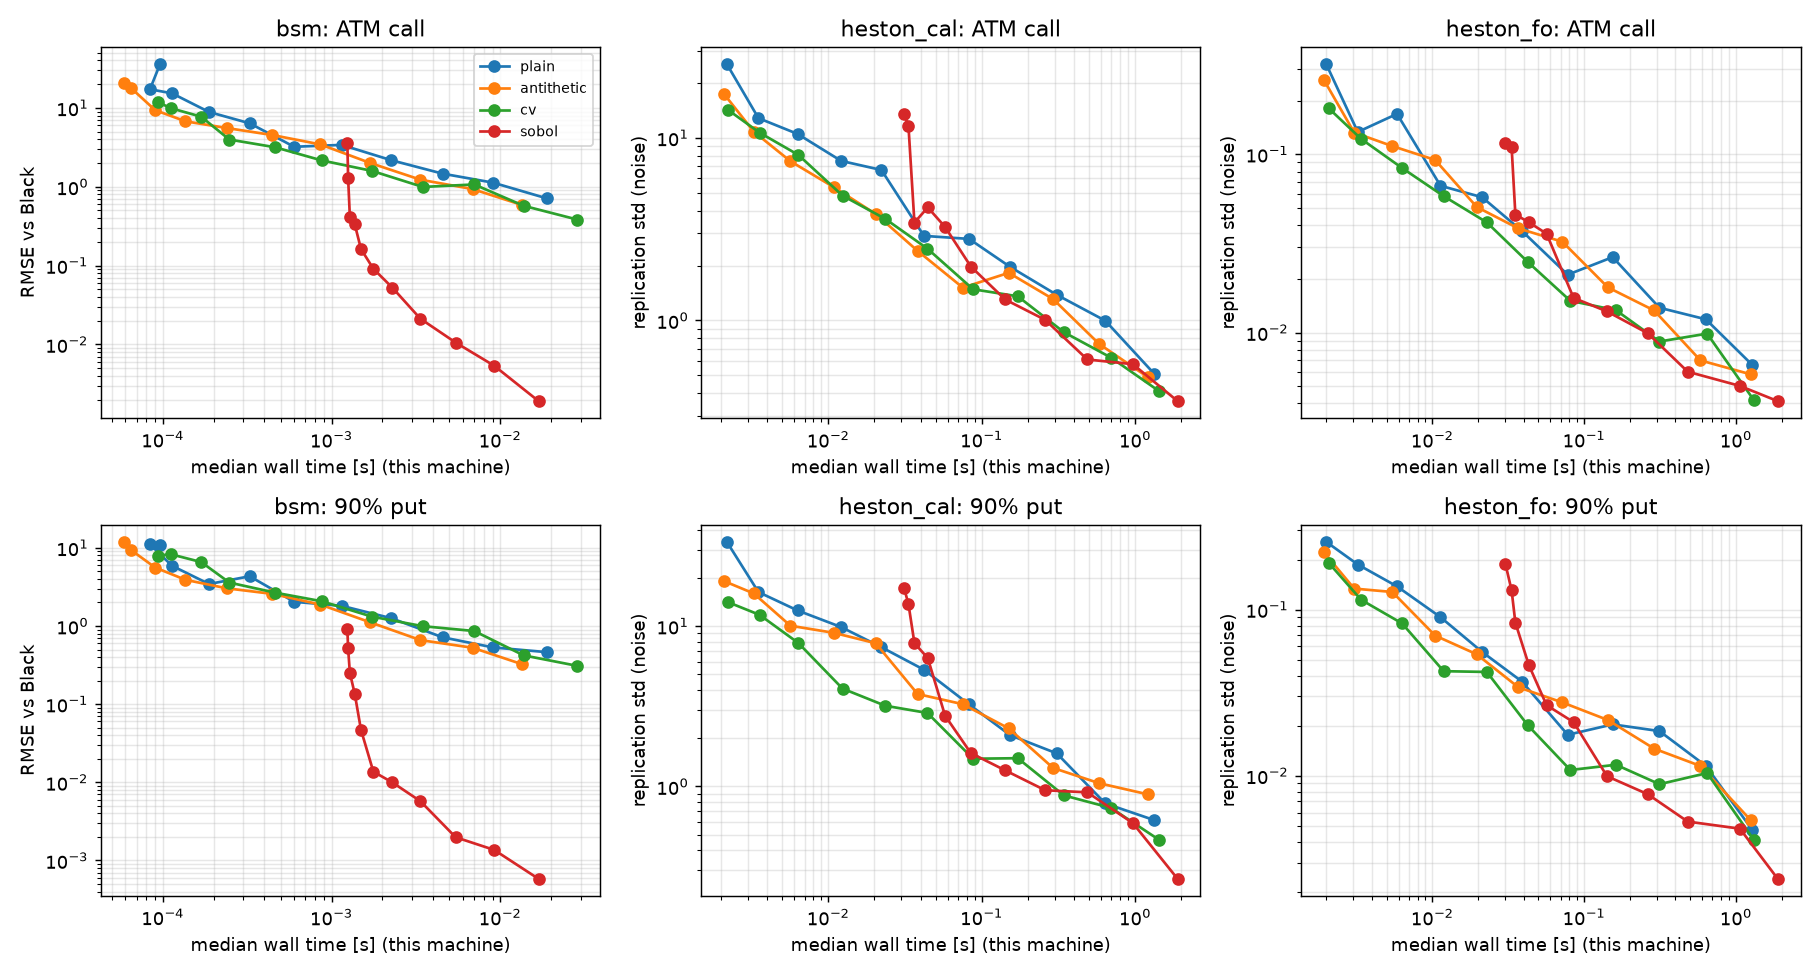
\includegraphics[width=\textwidth]{benchmark_time_vs_error.png}
\caption{Error (RMSE for bsm, standard deviation of the replications for Heston) against median computing time, for
the four methods, on a log-log scale. Times measured on a single machine.}
\label{fig:bm-tempo}
\end{figure}

Figure~\ref{fig:bm-tempo} plots the error as a function of time instead of $N$: it is the ``equal work'' comparison.
The almost vertical stretch of the Sobol' curve on the left has a trivial explanation: for small $N$ the time is
dominated by the construction of the 16 Sobol' generators (about 1 ms), not by the payoff computation.

\needspace{9\baselineskip}
\begin{attenzione}[title={Timings hold for one machine}]
The timings are serial medians on a single laptop, with the installed NumPy version: only the \emph{ratios} between
methods make sense off that machine. Even so they are noisy. Repeating the whole benchmark on the same machine, the
Heston efficiencies move by less than 10\%. Those of bsm move by 9--22\% (Sobol' $-22\%$), because the Black timings
are 14--29 milliseconds in this run (11--29 across runs) and are affected by every disturbance. The bsm efficiencies
should be read as indicative. The VRs, instead, depend only on the seeds and are bit-for-bit reproducible.
\end{attenzione}

\section{The QE-M discretization bias}
\label{sec:bm-bias}
\subsection{How it is measured}
The bias is the difference between the expected value of the scheme at a given step and the exact price:
$b(\Delta t)=\E\hat V_{\Delta t}-V_{\text{COS}}$. To see it, an SE much smaller than that of the benchmark is needed.
The procedure, declared in advance:
\begin{itemize}
\item estimator with the $F_T$ control variate (no additional bias, because QE-M is a martingale);
\item $8\times2^{20}\approx8.4\times10^6$ paths per level;
\item four steps: the base step times $\{\tfrac14,\tfrac12,1,2\}$, rounded up. For heston\_cal they are 9, 17, 34 and
68 steps; for heston\_fo 8, 16, 32 and 64;
\item the bias is also reported in \textbf{vol basis points} (1 bp $=0.01$ vol points), dividing by the Black vega at
the COS implied vol: about 0.295 per bp on the ATM call and 0.25 on the put.
\end{itemize}

\subsection{The full ladder}
On the heston\_cal set the same measurement was redone by an independent check with its own QE-M implementation; the
two estimates agree within 1.85 SE at all 8 points. Table~\ref{tab:bm-bias} reports the combined estimate of the two
runs.

\begin{table}[ht]
\centering
\small
\caption{QE-M bias on heston\_cal, $\hat V_{\Delta t}-V_{\text{COS}}$: combined estimate of the two independent runs,
in price units and in vol basis points. At step $T/17$ the put is about $-7$ SE.}
\label{tab:bm-bias}
\begin{tabular}{l r r r r}
\toprule
& \multicolumn{2}{c}{ATM call} & \multicolumn{2}{c}{90\% put}\\
\cmidrule(lr){2-3}\cmidrule(l){4-5}
$\Delta t$ & price & vol bp & price & vol bp\\
\midrule
$T/9$ & $+2.16\pm0.10$ & $+7.3$ & $+0.37\pm0.11$ & $+1.5$\\
$T/17$ & $+0.03\pm0.10$ & --- & $-0.80\pm0.11$ & $-3.2$\\
$T/34$ (benchmark) & $-0.17\pm0.10$ & $-0.6$ & $-0.40\pm0.11$ & $-1.6$\\
$T/68$ & $-0.23\pm0.10$ & $-0.8$ & $-0.28\pm0.11$ & $-1.1$\\
\bottomrule
\end{tabular}
\end{table}

\begin{figure}[ht]
\centering
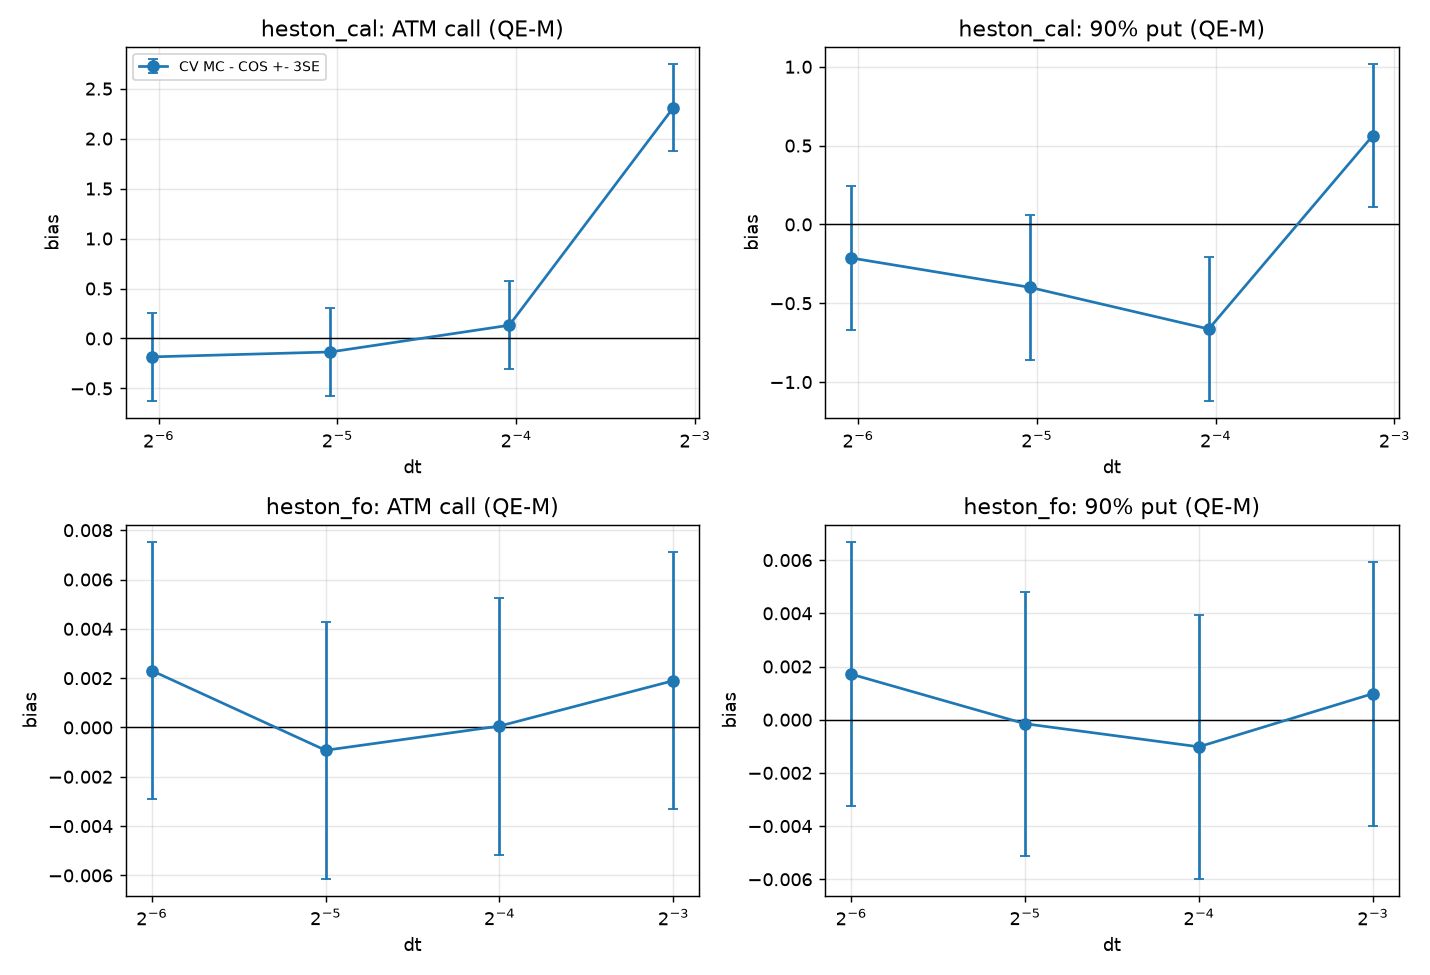
\includegraphics[width=0.9\textwidth]{benchmark_heston_bias.png}
\caption{QE-M bias (control-variate MC minus COS, bars $\pm3$ SE) against the step $\Delta t$, project run. Top:
heston\_cal, bottom: heston\_fo; left: ATM call, right: 90\% put.}
\label{fig:bm-bias}
\end{figure}

Table~\ref{tab:bm-bias} and Figure~\ref{fig:bm-bias} read as follows.
\begin{itemize}
\item \textbf{At the benchmark step ($T/34$)} the bias is small: $-0.6$ bp on the call and $-1.6$ bp on the put. Over
the whole fine ladder ($T/17$, $T/34$, $T/68$) it stays within about 3 bp. It is also smaller than the plain-MC SE at
$N=2^{20}$ (0.64 on the call, 0.80 on the put): it therefore cannot distort a 3 SE test on a single run. It becomes
visible only at the precision pooled over all replications: pooled plain MC minus COS is $-0.29$ ($-2.5$ SE) on the
call and $-0.30$ ($-2.1$ SE) on the put, over about $3.4\times10^7$ paths. This is precisely why the slope gate uses
the noise-only metric.
\item \textbf{At the coarse step $T/9$} the bias on the ATM call is large: $+2.31$ in the project run (15.9 SE,
$+7.8$ bp), $+2.02$ in the independent run, $+7.3$ bp combined. The step ($\Delta t\approx0.115$) is about half the
mean-reversion time $1/\kappa\approx0.22$, and with $\xi=1.65$ the variance moves a lot within a single step.
\item \textbf{The put is not monotonic in $\Delta t$}: $+0.37$, $-0.80$, $-0.40$, $-0.28$ as the step is halved. The
QE-M bias is not a simple $c\,\Delta t$ like that of Euler (Chapter~\ref{cap:mc}): it can change sign. The halving
differences between $T/17$, $T/34$ and $T/68$ stay within 1.3 SE, but this alone would hide the shape of the curve:
this is why the full ladder is reported.
\item \textbf{A non-robust point.} The put value at $T/9$ is $+0.56$ (3.7 SE) in the project run and $+0.17$ (1.1 SE)
in the independent one. Taken on its own, it is not a result.
\item \textbf{Set heston\_fo}: every level is within 1.33 SE of COS ($|b|\le0.0023$ on a price of 5.79). With
$\xi=0.58$ and Feller less violated the scheme is already exact within the noise at 8 steps.
\end{itemize}

\begin{idea}[title={Key idea: two errors, two measurements}]
Noise and bias are measured with different tools. Noise is measured from the dispersion of the replications and falls
as $N^{-1/2}$. Bias is measured with many more paths, at several steps, against an exact reference, and does not
depend on $N$. Mixing them in a single ``error against $N$'' curve makes the bias look like a slowdown of convergence.
\end{idea}

\section{Reproducibility}
\subsection{Deterministic regeneration}
All the figures and tables of the benchmark (the \path{benchmark_*} files in \path{report/figures/}) are written by a
single script, \path{scripts/run_benchmarks.py}. The script also writes a \emph{manifest}
(\path{benchmark_manifest.csv}) with, for each file: the sha256 hash, the size, the script that wrote it, the time of
the run and the configuration (``full'' or ``quick''). The reproducibility gate checks that:
\begin{itemize}
\item every listed file exists and has the recorded hash (12 files out of 12);
\item the configuration is the full one;
\item there are no unlisted \path{benchmark_*.png} figures (0 stray files).
\end{itemize}

\begin{attenzione}[title={Integrity is not provenance}]
The manifest is written by the very script one wants to verify, and the ``written by'' field is a string. A matching
hash only shows that the files have not changed \emph{after} the run (integrity). It does not show that they were
produced by that code (provenance).

Provenance is shown in another way: by re-running. An independent check re-ran the whole \path{run_benchmarks.py} in
a separate folder, with 6 processes instead of 8 (218 s). Result:
\begin{itemize}
\item bit-for-bit identical: the three convergence figures, the bias figure, and the tables of references,
convergence, bias and control choice;
\item in the table of runs, every price and every SE bit-for-bit identical; only the timings change;
\item different, as expected, only the outputs that depend on timings: the time--error figure, the timing table and
the time and efficiency columns of the summary.
\end{itemize}
The project's two full runs (216 s and 294 s, different machine load) also have bit-for-bit identical prices and SEs.
\end{attenzione}

\subsection{Declared in advance, but how do we know?}
The procedure (cases, grid, replications, seeds, metrics, gates) was written before the full run. But it was committed
to version control together with the results, so the repository history alone does not prove it. That there was no
selection is shown by three facts:
\begin{itemize}
\item the procedure leaves nothing to choose: all 11 points, all 6 pairs, both fits, a fixed formula for the seeds;
\item with fresh seeds, 0 slopes out of 104 fall outside the band, with standard deviations (0.014--0.032) much
smaller than the half-width of the band (0.1);
\item the independent re-run is bit-for-bit identical.
\end{itemize}

\begin{progetto}[title={In the qpricer project: the benchmark files}]
\begin{itemize}
\item \path{src/qpricer/engines/vr.py}: the function \code{vanilla\_mc}, which implements the four methods
(\code{plain}, \code{antithetic}, \code{cv} and \code{sobol}), plus the helper functions for the antithetic pairs and
for the Sobol' normals. Every pricer returns \code{(price, SE, N, seed)}.
\item \path{scripts/run_benchmarks.py}: cases, references, parallel runs, serial timing pass, bias and control-choice
studies, figures and manifest. The \code{-{}-quick} option runs a minimal grid for the tests.
\item \path{scripts/phase6_gates.py}: the 52 checks, read from the files on disk.
\end{itemize}
\end{progetto}

\begin{riassunto}
\begin{itemize}
\item Benchmark on an SPX point close to one year (Black at the Heston ATM vol, calibrated Heston) and on the
Fang--Oosterlee set; COS reference, checked against Lewis and independent Gil-Pelaez to better than $10^{-8}$.
\item $N^{-1/2}$ slope: fit a metric over the replications (RMSE, or the dispersion for Heston, to exclude the bias),
never the error of one run (too noisy) nor the SE (slope $-0.5$ by construction). Measured: from $-0.554$ to $-0.487$;
104 trials with fresh seeds between $-0.558$ and $-0.445$.
\item Antithetics: VR $=1/(1+\rho_A)$, they remove the odd part of the payoff and leave the convexity; SE from the
pairs. $F_T$ control: exact mean even under QE-M, bias of the estimated $\hat\beta$ $O(1/N)$, better than the shadow
Black. Randomized Sobol': order about $N^{-1}$ in one dimension, only a constant factor at 64--68 dimensions; SE from
16 scramblings, right on average but with heavy tails.
\item For the same time, under Heston: $F_T$ control 2.2--3.2, Sobol' 2.3--4.8, antithetics 1.2--1.5.
\item QE-M bias at step $T/34$: $-0.6$ and $-1.6$ bp; at $T/9$ up to $+7.3$--$7.8$ bp on the ATM call; non-monotonic
on the put.
\item The sha256 manifest proves integrity; the bit-for-bit identical independent re-run proves provenance.
\end{itemize}
\end{riassunto}

\begin{domande}
\begin{enumerate}
\item Why does the slope gate for Heston use the standard deviation of the replications and not the RMSE against COS?
\item Why is the slope of the error of a single run too noisy for a gate? Roughly what is its standard deviation over
11 points?
\item Why is the slope of the SE $-0.5$ even for wrong code? Which check does have power?
\item Show that antithetics have $\mathrm{VR}=1+\Var g_o/\Var g_e$. When do they make things worse?
\item Why does the $F_T$ control variate introduce no discretization bias under QE-M? What would happen with plain QE?
\item Where does the $O(1/N)$ bias of the estimated coefficient come from, and why is it negligible?
\item Why does Sobol' converge at about $N^{-1}$ under Black and almost at $N^{-1/2}$ under Heston?
\item Why does the $t$ statistic of the 16 scramblings exceed 3 more often than expected? What does this imply for the
tests?
\item Why does adding a uniform inside the $2^{-30}$ cell neither introduce bias nor break the net?
\item What is the difference between the integrity and the provenance of a result? What does each one prove?
\end{enumerate}
\end{domande}

\chapter{How the results are verified}
\label{cap:validazione}

A price is useful only if one knows \emph{why} it is right. This chapter closes this document by gathering in one place the
verification method used throughout the project, the results of each phase, the cases in which verification found an
error, the limitations that remain open and the commands to redo everything from scratch.

\section{The verification principles}
\subsection{Four kinds of evidence}
Each phase of the project is considered complete only when its \emph{gates} pass: numerical checks with a tolerance
fixed in advance. The gates are of four kinds.
\begin{enumerate}
\item \textbf{Two independent methods agree} within a stated tolerance: closed form against Fourier against Monte
Carlo, COS against Lewis, Brownian bridge against the reflection principle. ``Independent'' means that they do not
share approximations: if they are wrong, they are wrong in different ways.
\item \textbf{Limiting cases reproduce a simpler model}: Heston with $\xi\to0$ gives Black, SABR with $\nu\to0$ gives
a flat volatility, an Asian with a single fixing is a vanilla, Heston with $\xi=10^{-4}$ prices barriers and
autocallables like Black.
\item \textbf{No-arbitrage identities hold}: put--call parity, knock-in plus knock-out equals vanilla, monotonicity and
convexity in $K$, absence of calendar arbitrage.
\item \textbf{Monte Carlo comparisons are expressed in standard errors}: a test passes if $|z|\le3$ (Chapter~\ref{cap:mc}), and the error must fall as $N^{-1/2}$ (Chapter~\ref{cap:benchmark}).
\end{enumerate}

\subsection{Multiple tests and false alarms}
A ``3 SE'' test fails with correct code with probability $0.27\%$. With $m$ independent tests the probability of at
least one false alarm is $1-0.9973^m$ \eqref{eq:test-multipli}: about 5\% for $m=20$, 16\% for $m=66$. The project
follows three rules.
\begin{itemize}
\item \textbf{The false-alarm rate is written down in advance.} In this way an isolated failure between 3 and 3.5 SE is
read as expected multiplicity and diagnosed, instead of being ``fixed'' by changing the seed.
\item \textbf{Seeds are fixed and declared in advance.} Changing the seed until the test passes is equivalent to
loosening the tolerance.
\item \textbf{The actual rate is measured.} When the tests are correlated or the reference is approximate, the formula
$1-0.9973^m$ does not hold: the gate is repeated with many fresh seeds and the failures are counted. For SABR, for
example, 100 fresh seeds on 21 comparisons give 4.0\% of failed seeds.
\end{itemize}

\subsection{Tolerances fixed and never loosened}
The hard rules are few.
\begin{itemize}
\item A tolerance is never loosened, a test is never skipped, an input is never tweaked to make a test pass.
\item If a test fails, the mathematics is suspected first (conventions, signs, measure), then the code, and the test
last.
\item If the test itself is ill-posed (Section~\ref{sec:val-lezioni} shows two such cases), it is replaced with a check
that is \emph{at least as strict}, and the replacement is documented.
\item No number is written by hand: every number comes from a script in the repository and can be regenerated.
Synthetic data are always labelled as such.
\end{itemize}

\subsection{Independent reimplementation}
The strongest guarantee comes from a second verification, separate from the development of the code. For each phase an
independent check:
\begin{itemize}
\item read the mathematical specification, not the code under verification;
\item wrote its own reference code, which imports nothing from the library: its own Black formula, its own Heston
characteristic function with Gil-Pelaez or Lewis, its own \mbox{QE-M} scheme with a different ordering of the random
numbers, its own settlement-time computation, its own parity regression;
\item used its own seeds, declared in advance and never changed after seeing a result;
\item left a test \emph{deliberately failing} for each defect found, as a reproduction, until the defect was fixed.
\end{itemize}
These tests live in \path{tests/validation/} and are part of the full suite. The reference values produced in this
way, with their source stated, are frozen in \path{tests/golden/} and are never modified.

\begin{attenzione}[title={The tautological test}]
A test that cannot fail verifies nothing. The typical examples are computing the put from the call by parity and then
``verifying'' parity, or defining the knock-in as vanilla minus knock-out and then ``verifying'' that the sum gives the
vanilla. The project prices the two legs with separate calls and compares different engines. Section~\ref{sec:val-lezioni} recounts two tautological gates that slipped through the first draft and were found by the
independent check.
\end{attenzione}

\section{The results, phase by phase}
Table~\ref{tab:val-gate} lists all the gates, with the \emph{final} measured value, that is, after the fixes described
in Section~\ref{sec:val-lezioni}. The ``reported'' rows are documented measurements without a threshold. The phases
are:
\begin{itemize}[leftmargin=4.2em,labelwidth=3.4em,labelsep=0.8em,align=left]
\item[Phase 0] SPX data: cleaning, $F$ and $\DF$ from parity (Chapter~\ref{cap:dati});
\item[Phase 1] Black-76: price, Greeks, implied volatility (Chapter~\ref{cap:black});
\item[Phase 2] Heston: COS, Lewis, Monte Carlo (Chapters~\ref{cap:heston} and~\ref{cap:mc});
\item[Phase 3] SABR (Chapter~\ref{cap:sabr});
\item[Phase 4] exotics: barriers, Asians, autocallables (Chapters~\ref{cap:barriere}--\ref{cap:autocallable});
\item[Phase 5] calibration to the SPX (Chapter~\ref{cap:calibrazione});
\item[Phase 6] Monte Carlo versus formulas benchmark (Chapter~\ref{cap:benchmark}).
\end{itemize}

{\small
\setlength{\LTcapwidth}{\textwidth}
\begin{longtable}{@{}>{\raggedright\arraybackslash}p{6.2cm}>{\raggedright\arraybackslash}p{4.6cm}
>{\raggedright\arraybackslash}p{2.6cm}>{\raggedright\arraybackslash}p{1.1cm}@{}}
\caption{All the project gates with the final measured value.}\label{tab:val-gate}\\
\toprule
gate & measured & tolerance & result\\
\midrule
\endfirsthead
\toprule
gate & measured & tolerance & result\\
\midrule
\endhead
\midrule
\multicolumn{4}{r}{\emph{continued}}\\
\endfoot
\bottomrule
\endlastfoot
\multicolumn{4}{@{}l}{\textbf{Phase 0: SPX data}}\\
$R^2$ of the parity line, every kept expiry & min 0.999941 (39 of 39) & $>0.999$ & pass\\
Expiry failing the filters: discarded and logged & only \mbox{2026-12-08} (7 pairs) & discard + log & pass\\
Implied $\DF$, every kept expiry & $[0.923895,\,0.998395]$ & $(0.8,1]$ & pass\\
$T$ (ACT/365F, settlement times, early closes) against independent clock
& $\max|\Delta T|=0$ on 40 expiries & $10^{-12}$ & pass\\
Second method (L1 regression, no discards) & $\max|\Delta F|/\SE_F=1.87$ & $<3$ & pass\\
Calibration surface free of strict static arbitrage & 0 (7650 $\to$ 7625 quotes) & 0 & pass\\
AM against PM forwards on the common dates & 0.27 index points & $<0.4$ & pass\\
\midrule
\multicolumn{4}{@{}l}{\textbf{Phase 1: Black-76}}\\
Put--call parity, $K/F\in[0.25,4]$ & $1.14\times10^{-13}$ & $10^{-12}$ & pass\\
Implied volatility, round trip (OTM input) & $1.07\times10^{-14}$ & $10^{-10}$ & pass\\
Implied volatility, round trip (ITM input) & $8.23\times10^{-13}$ & $10^{-10}$ & pass\\
Delta and vega against finite differences & $\le2.96\times10^{-7}$ & $10^{-5}$ & pass\\
OTM gamma against finite differences & $9.96\times10^{-7}$ & $10^{-5}$ & pass\\
Theta (joint bump of $T$ and $\DF$) & $1.69\times10^{-8}$ & $10^{-5}$ & pass\\
\midrule
\multicolumn{4}{@{}l}{\textbf{Phase 2: Heston}}\\
COS against Lewis, 4 sets, $K\in[60,150]$, $T\in[0.1,3]$ & $1.83\times10^{-10}$ & $10^{-6}$ & pass\\
COS against Lewis, 300 random sets $\times$ 6 expiries & 0 cells out of 1800 over threshold; max
$3.05\times10^{-9}$ & $10^{-6}$ & pass\\
$\xi=10^{-4}$, $\rho=0$, against Black at the integrated variance & $4.36\times10^{-8}$ & $10^{-5}$ & pass\\
$\xi=10^{-4}$, $\rho=-0.7$, against Black plus the $\rho\xi$ term & $5.58\times10^{-8}$ & $10^{-5}$ & pass\\
QE and QE-M against COS, 24 comparisons & $\max|z|=0.71$ & 3 & pass\\
Same comparisons, 20 fresh seeds (480 values of $z$) & $\max|z|=2.86$; mean $-0.115$, sd 0.937 & 3 & pass\\
Published Fang--Oosterlee value (ATM call) & $-1.6\times10^{-8}$ & reported & --\\
\midrule
\multicolumn{4}{@{}l}{\textbf{Phase 3: SABR}}\\
$\nu\to0$, $\beta=1$: flat volatility $\alpha$ & $3.0\times10^{-12}$ & $10^{-10}$ & pass\\
Hagan against MC, 21 comparisons, $\nu^2T\le0.16$ & $\max|z|=1.68$ & 3 & pass\\
Step bias of the log-Euler scheme, $|d|/\SE_{\text{gate}}$, three expiries & max 0.080 & 0.1 & pass\\
Order check $M(\hat V_{1/M}-\hat V_{1/2M})$ & flat within the noise & reported & --\\
Identities of the Hagan formula (jump, symmetry, quadrature) & $\le4.7\times10^{-14}$
& $10^{-11}$--$10^{-14}$ & pass\\
Robustness: 100 fresh seeds $\times$ 21 comparisons & 4.0\% of seeds failed & reported & --\\
\midrule
\multicolumn{4}{@{}l}{\textbf{Phase 4: exotics}}\\
Knock-in + knock-out = vanilla, 8 types, Black and Heston & $3.55\times10^{-15}$ & $10^{-12}$ & pass\\
Barriers, bridge MC against formula, 4 configurations $\times$ 14 cells & $\max|z|=1.99$ & 3 & pass\\
Barriers under Heston with $\xi=10^{-4}$, $\rho=0$ & $|z|=2.97$ & 3 & pass\\
Down-and-out with $K=H$ under Heston (model-free identity) & $z=0.75$ & 3 & pass\\
Continuous and BGK-shifted formulas against BGK tables & $4.97\times10^{-4}$ & $5\times10^{-4}$ & pass\\
Discrete MC against exact BGK values, 13 cells & ${\max|d|/(3\SE+10^{-3})=0.54}$ & 1 & pass\\
Haug table, 66 correctly rounded cells & $4.96\times10^{-5}$ & $5\times10^{-5}$ & pass\\
Haug table, 6 wrong cells against independent values & $3.46\times10^{-14}$ & $10^{-10}$ & pass\\
Geometric Asian, MC against Kemna--Vorst, 39 cells & $\max|z|=1.90$ & 3 & pass\\
Kemna--Vorst against published table & $1.28\times10^{-4}$ & $3\times10^{-4}$ & pass\\
Arithmetic Asian with control against published table & ${\max(|d|-3\SE)/(3\cdot10^{-4})}={-1.21}$ & 1 & pass\\
Other Asian MC checks (means, independent seeds, $\xi=10^{-4}$) & $\max|z|=1.45$ & 3 & pass\\
Autocallable, Black: MC against formulas & $\max|z|=1.79$ & 3 & pass\\
Autocallable, Heston: martingale, digitals against COS, no autocall & $\max|z|=1.32$ & 3 & pass\\
Autocallable, Heston with $\xi=10^{-4}$ against Black (same random numbers) & $|z|=0.18$ & 3 & pass\\
Quarterly autocallable, calibrated Heston: legs against exact values & $\max|z|=0.87$ & 3 & pass\\
\quad Heston $-$ Black difference & $-0.01869$ (SE 0.00022) & reported & --\\
Annual autocallable, calibrated Heston: legs against exact values & $\max|z|=1.19$ & 3 & pass\\
\quad Heston $-$ Black difference & $-0.02514$ (SE 0.00034) & reported & --\\
\midrule
\multicolumn{4}{@{}l}{\textbf{Phase 5: calibration}}\\
COS at fixed $(N,L)$ against Lewis over the box, in units of market vega & $9.21\times10^{-6}$ & $10^{-5}$ & pass\\
Short-end rate curve: identity and pairs inside the band & $\max|\text{res}|/h=0.834$ & 1 & pass\\
Black at the market vol reproduces the price (7625 quotes) & $3.9\times10^{-13}$ & $10^{-12}$ & pass\\
Heston synthetic round trip, no noise (two sets) & $\le4.1\times10^{-14}$ & $10^{-6}$ & pass\\
Heston synthetic round trip, parameters within 3 SE & $\max|z|=2.42$ & 3 & pass\\
Heston synthetic round trip, distance $D^2$ & 2.52 and 12.49 & 20.52 & pass\\
Linearization, 64 seeds: $\mathrm{sd}(\hat p_j)/\SE_j$ & from 0.98 to 1.20 & $[0.73,1.27]$ & pass\\
SABR synthetic round trip, 4 expiries: $D^2$ & max 5.41 & 16.27 & pass\\
Real fit: converging starts & 16 of 16, a single basin & $\ge8$ & pass\\
Real fit: fallbacks at the optimum, finite residuals & 0; yes & 0; yes & pass\\
COS against Lewis at the fit, in volatility & $4.9\times10^{-13}$ & $10^{-5}$ & pass\\
Price objective against vol objective: $|\Delta p|/\SE$ & max 0.83 & 1 & pass\\
RMSE table & 39 rows, 0 NaN & 0 NaN & pass\\
Real surface: strict butterflies between adjacent strikes & 0 & 0 & pass\\
\midrule
\multicolumn{4}{@{}l}{\textbf{Phase 6: benchmark}}\\
COS against Lewis, relative to the smallest SE & $7.36\times10^{-9}$ & $3.09\times10^{-5}$ & pass\\
Slope of the error metric, 6 cases & from $-0.554$ to $-0.487$ & $[-0.6,-0.4]$ & pass\\
Slope of the SE, 6 cases (consistency only) & from $-0.505$ to $-0.499$ & $[-0.6,-0.4]$ & pass\\
Slopes with fresh seeds, independent check (104) & from $-0.558$ to $-0.445$ & $[-0.6,-0.4]$ & pass\\
Plain MC within 3 SE at every $N$, 66 comparisons & $\max|z|=2.90$ & 3 & pass\\*
Antithetics, control and Sobol' unbiased, 20 comparisons & $\max|z|=2.01$ & 3 & pass\\*
Regeneration: sha256 hashes, configuration, stray files & 12 of 12; 0 stray & exact & pass\\
\end{longtable}
}

\needspace{10\baselineskip}
\begin{progetto}[title={In the qpricer project: the overall numbers}]
\begin{itemize}
\item The gate scripts print 28 rows for phase 4, 35 for phase 5 and 52 for phase 6, all passed.
\item The full suite has 599 tests, all passed, none skipped or marked as an expected failure (about 18 minutes on a
laptop, slow tests included).
\item The code is checked with \code{ruff check} and \code{ruff format}, with no warnings.
\end{itemize}
\end{progetto}

\section{What verification found}
\label{sec:val-lezioni}
The following cases are always told in the same order: the \emph{symptom} (what was seen), the \emph{cause} (why), the
\emph{fix} (what changed). None of them was resolved by loosening a tolerance.

\subsection{COS truncation}
\begin{description}
\item[Symptom.] With the truncation interval at 12 standard deviations, the COS error against Lewis did not fall as
the number of series terms grew (same error with ${N=256}$ and ${N=4096}$) and missed the $10^{-6}$ gate on the FO
($3.95\times10^{-5}$) and GS ($2.58\times10^{-6}$) sets. With the interval widened to 18 standard deviations, the four
gate sets passed. But an independent check tried 300 random parameter sets plausible for the SPX, on 6 expiries: 413
cells out of 1800 (22.9\%) over $10^{-6}$, up to $9.95\times10^{-2}$, and 5 of these without any warning.
\item[Cause.] Truncation error, not series error. With $\rho<0$ the left tail of $\ln F_T$ is heavy, and the COS
reflection term grows like $e^{-y}$ precisely there. The code's warning estimated only the series error.
\item[Fix.] COS became \emph{self-checking}: it compares $(N,L)$ with $(2N,L+6)$ and doubles until the two estimates
agree within $10^{-9}F$; if it does not converge by $N=2^{14}$ it warns, and it never returns a silent error. On the
same scan: 0 cells out of 1800 over threshold, maximum error $3.05\times10^{-9}$.
\end{description}

\subsection{\texorpdfstring{The $\xi\to0$ limit was misspecified}{The xi -> 0 limit was misspecified}}
\begin{description}
\item[Symptom.] The gate ``with $\xi=10^{-4}$ Heston coincides with Black at the integrated variance within $10^{-5}$''
passed at $\rho=0$ ($2.6\times10^{-8}$) and failed at $\rho=-0.7$ ($3.27\times10^{-4}$). The gap was linear in $\xi$:
$3.27\times10^{-3}$, $3.27\times10^{-4}$, $3.25\times10^{-5}$ for $\xi=10^{-3},10^{-4},10^{-5}$.
\item[Cause.] With $\rho\ne0$ the difference between Heston and Black is \emph{first} order in $\rho\xi$: it is the
skew term. The gate, as written, was unreachable by any correct code: a specification error.
\item[Fix.] The gate is run at $\rho=0$ against Black (tolerance unchanged) and at $\rho=-0.7$ against Black
\emph{plus} the first-order term in $\rho\xi$, with the same tolerance: $4.36\times10^{-8}$ and $5.58\times10^{-8}$.
The shortcut ``just take $\xi=10^{-7}$'' was rejected: the $\kappa\theta/\xi^2$ terms of the characteristic function
cancel catastrophically, and one would be testing rounding instead of the model.
\end{description}

\subsection{Three hours too many: the early close}
\begin{description}
\item[Symptom.] For the expiry \mbox{2026-11-27} the check's independent clock disagreed with the code's $T$. The
first comparison excluded precisely that expiry.
\item[Cause.] 27 November 2026 is the day after Thanksgiving: the exchange closes at 13:00, and SPXW options expire at
13:00 instead of 16:00. Three hours of error on a time to expiry of about three weeks.
\item[Fix.] The early-close calendar (day after Thanksgiving, 3 July and 24 December when they are trading days) was
added to the settlement-time computation. Now $T$ agrees on \emph{all} 40 expiries within $10^{-12}$, with no
exclusions ($T=0.0570512$ for that date).
\end{description}

\subsection{\texorpdfstring{The solver that silently returned $\sigma=0$}{The solver that silently returned sigma = 0}}
\begin{description}
\item[Symptom.] For OTM prices below about $10^{-280}$ the implied-volatility solver returned a wrong vol, even
$\sigma=0$, with an ``all good'' status code. Example: $V=2.162\times10^{-305}$, $F=100$, $K=100\,e^{38.5\sqrt5}$,
$T=5$: $\hat\sigma=0$, while the true one is 1.
\item[Cause.] The library's normal cumulative distribution function returns 0 for $d\lesssim-37.5$, even though
$\Phi(d)$ is representable down to about $-38.5$. In that range the normalized price loses its second term, and the
solver converges, correctly, on the wrong function. No final check rejected $\sigma=0$.
\item[Fix.] In those cases NaN is returned with a dedicated status code and a warning. No effect on the SPX data, where
such prices do not exist; but the rule ``never a silently wrong number'' applies everywhere.
\end{description}

\subsection{The SABR step bias at short expiries}
\begin{description}
\item[Symptom.] The step-halving test with common random numbers had been rightly replaced by a size check,
$|\hat V_\Delta-\hat V_{\Delta/2}|\le0.1\,\SE_{\text{gate}}$ (Section~\ref{sec:halving}). But it had been checked only
at $T=1$ (0.073). The independent check, with exact expected values, found 0.321 at $T=0.25$ and 0.160 at $T=0.5$,
with a bias of $-0.0415$ vol points (0.64 SE) in the left wing.
\item[Cause.] The step was fixed in calendar time ($\Delta=1/250$), so at $T=0.25$ there were only 63 steps. Applying
a criterion only where it passes is loosening by omission.
\item[Fix.] 250 steps at every expiry ($\Delta=T/250$). The ratio is now at most 0.080, 0.063 and 0.073 at the three
expiries, and the bias is at most 0.17 SE.
\end{description}

\subsection{The wrong digits in the Haug table}
\begin{description}
\item[Symptom.] Six cells of the Haug barrier table (column $\sigma=0.30$) were between $5.2\times10^{-5}$ and
$6.3\times10^{-5}$ away from the reflection formula, beyond the tolerance of $5\times10^{-5}$ (half a unit of the last
printed digit).
\item[Cause.] The six cells are not correctly rounded: the formula, an independent quadrature and a PDE agree with
each other to better than $10^{-9}$. The first fix, however, had moved the \emph{whole} column to $10^{-4}$: this
loosened the tolerance also for 30 cells that passed at $5\times10^{-5}$.
\item[Fix.] Cells handled one by one: the 66 correct ones stay at $5\times10^{-5}$ (maximum $4.96\times10^{-5}$), the
6 wrong ones are compared with independently computed reference values at $10^{-10}$ ($3.46\times10^{-14}$). No
tolerance was loosened.
\end{description}

\subsection{The default grid of the Asians under Heston}
\begin{description}
\item[Symptom.] With quarterly fixings under Heston, the default Asian price differed from the one with step $1/32$
by $z=-2.6$, $-3.6$ and $+5.9$ at $K=90$, 100 and 110 ($+0.0133$, that is 1.3\%, at $K=110$; $3\times10^6$ paths).
\item[Cause.] By default the code took a single QE-M step per fixing period (a quarter of a year), against the project
rule of a step of at most $1/32$.
\item[Fix.] Maximum step $1/32$ by default, as already for the autocallables; with $2\times10^6$ paths the three $z$
become $-1.08$, $-1.25$ and $-1.14$. The coarse grid remains available only if explicitly requested.
\end{description}

\subsection{The tautological gate}
\begin{description}
\item[Symptom.] In the attribution of the autocallable Heston--Black difference (Chapter~\ref{cap:autocallable}), a
gate required the three terms to add up to the total difference within $10^{-12}$. It always passed.
\item[Cause.] The third term was \emph{defined} as the residual difference, so the sum equalled the total by
construction: that half of the gate could not fail.
\item[Fix.] The identity was replaced by real checks: each leg against an exact value within 3 SE (maximum $|z|$ 0.87
and 1.19). The total difference and the three terms were also recomputed independently (for example exact Black
1.014493 against MC 1.014530, $z=0.40$). The same kind of problem surfaced in the benchmark: the slopes fitted on the
SE are $-0.5$ by construction and were downgraded to a consistency check (Chapter~\ref{cap:benchmark}).
\end{description}

\begin{idea}[title={Key idea: what these cases teach}]
Almost all the defects found lay \emph{outside} the test cases chosen at the start: random parameters instead of the
four literature sets, the expiry excluded from the comparison, the extreme price, the short expiry, the default
setting. A gate says something only about the domain on which it was tried; widening the domain is the most effective
way to find errors.
\end{idea}

\section{Known limitations and open points}
\label{sec:val-limiti}
\begin{itemize}
\item \textbf{Published Heston values not reproduced (Albrecher and coauthors).} Lewis and COS, which agree with each
other, differ from the published ATM calls on the FO set by $+0.0043$, $+0.0073$, $-0.0007$, $+0.0052$ and $+0.0019$
at $T=1,2,3,5,10$, against a stated accuracy of 0.005: two expiries miss it. It is not a convention (no single rate
reproduces them all). The most likely explanation is that the authors used unrounded parameters: rounding the five
printed parameters by half a unit moves the prices by more than the stated accuracy. The same characteristic function
reproduces other published values to $1.6\times10^{-8}$ or better. These values are not used as binding tests.
\item \textbf{Autocallable of Deng and coauthors, case 2, not reproduced.} Published value 98.39; the project MC gives
97.508 (SE 0.009) and an independent exact backward induction 97.507: about 100 SE apart. Case 1 and the published
first-redemption probabilities are reproduced ($\max|z|=2.11$). The cause is unknown (perhaps a different coupon or
protection convention, perhaps the finite-difference error of the original paper). Nothing was tweaked to make it
match, and the value is not used as a reference.
\item \textbf{Implied volatility from deep ITM quotes.} Outside the test domain, for ITM quotes with $3<|z|<7.5$, the
solver returns a vol with an error of up to $2\times10^{-4}$ without flagging it. It is the conditioning limit of the
input: an ITM quote carries its time value only down to $\varepsilon\max(F,K)$. No effect on the results, because only
OTM quotes are inverted (error $\le10^{-14}$).
\item \textbf{SABR outside the validated domain.} Hagan was compared with MC only for $\nu^2T\le0.16$. All 39
expiry-by-expiry SABR fits have $\nu^2T$ between 0.352 and 0.890, and with $\nu\approx1$ Hagan is off by $+0.40$ vol
points ($T=0.5$) and $+0.82$ ($T=1$) at $k=-0.2$. Those smiles should be read as Hagan parametrizations, not as SABR
dynamics (Chapter~\ref{cap:sabr}).
\item \textbf{Heston does not fit the short expiries.} Out of sample ($T<0.1$, 18 expiries) the aggregate RMSE is
1.379 vol points (0.832--2.093 per expiry), with a maximum deviation of 6.29 points on the shortest expiry. It is
structural: the Heston skew does not grow enough as $T\to0$ (Section~\ref{sec:cal-skew}).
\item \textbf{Curvature SEs underestimate model risk.} The residuals are about 2.7 half-spreads ($s^2=7.37$), and
changing the expiry window moves $\kappa$ and $\xi$ by about 13 SE. The parameter uncertainty should therefore be read
from the range of the variants, not from $\pm\SE$ (Chapter~\ref{cap:calibrazione}).
\item \textbf{Reference level of the autocallable.} The level $S_{\text{ref}}$ still uses the parity $\DF$ of the
first expiry, not the smooth curve: $+0.074\%$ on the level (from 7374.425 to 7379.918). The estimated effect on the
quarterly Heston--Black difference is $-8\times10^{-5}$, about 0.4 SE. It is a minor point, not yet fixed.
\item \textbf{Code size.} The core in \path{src/} has 2644 lines, against an initial target of about 1500. Modules
already validated were not rewritten to shorten them, so as not to invalidate their verification.
\item \textbf{Sobol' and single-run tests.} The SE from 16 scramblings is calibrated on average, but its $t$ statistic
has heavy tails: no ``3 SE'' test on a single Sobol' run (Chapter~\ref{cap:benchmark}).
\end{itemize}

\section{Reproducibility}
\subsection{The data}
The raw snapshot of the SPX option chain (6 November 2026, 22:13 UTC) is not distributed with the repository: it is a
file excluded from version control. What is distributed are the processed files in \path{data/processed/}: the table
of $F$ and $\DF$, the cleaning counts, the OTM surface, the quotes removed for arbitrage and the calibrated Heston
parameters.

Two levels of reproducibility follow.
\begin{itemize}
\item Everything that starts from the processed files (benchmark, exotics, SABR and Heston figures) is regenerated
identically.
\item What starts from the raw quotes (market construction, calibration, tests on real data) requires the snapshot.
Without it one can download a new one; the numbers will be those of a different market day. The tests on real data,
if the snapshot is missing, fail instead of being skipped.
\end{itemize}

\subsection{The commands}
From the repository root, with the project's virtual environment (\code{.venv/bin/python}, abbreviated here to
\code{python}):
{\small
\begin{verbatim}
# data (optional: requires the network, produces a new snapshot)
python scripts/fetch_spx.py
python scripts/build_market.py

# gates of each phase
python scripts/phase1_gates.py      # ... up to
python scripts/phase6_gates.py

# results and figures
python scripts/run_calibration.py --workers 8
python scripts/autocall_compare.py \
    --heston-params data/processed/heston_fit_20261106_2213.json
python scripts/exotics_figures.py
python scripts/sabr_degradation.py
python scripts/heston_euler_bias.py
python scripts/run_benchmarks.py --workers 8

# tests
pytest -m "not slow" -q             # fast
pytest -q                           # all
\end{verbatim}
}

Practical notes.
\begin{itemize}
\item Every Monte Carlo script uses fixed seeds written in the code: re-running it gives the same numbers bit for bit,
regardless of the number of processes.
\item Computing times (and only those) change from one run to another and from one machine to another.
\item The independent checks are in \path{tests/validation/}; run directly, each file prints the numbers it checked.
\end{itemize}

\section{The development method}
The code was generated with a pipeline of artificial-intelligence agents (Claude Code). The author specified the
project (models, products, conventions, acceptance criteria) and supervised the mathematics and the validation. No
result rests on trust in the generator: every reported number is produced by a script in the repository, is covered
by automated tests with tolerances fixed in advance, and was rechecked by independent reimplementations that share no
code with the library.

\begin{riassunto}
\begin{itemize}
\item Four kinds of evidence: two independent methods, limiting cases, no-arbitrage identities, Monte Carlo in SE
units. False-alarm rate declared in advance, fixed seeds, tolerances never loosened.
\item Each phase was rechecked by a separate verification with its own reference code; all gates pass with the final
values of Table~\ref{tab:val-gate}.
\item Verification found eight significant problems, almost all outside the initial test cases: COS truncation,
ill-posed $\xi\to0$ gate, early close, silent ${\sigma=0}$, SABR step bias, Haug digits, Asian grid, tautological
gates.
\item Still open: two published values not reproduced, implied vol from deep ITM quotes, SABR outside its domain, the
Heston fit at the short end, curvature SEs, the autocallable reference level, 3 SE tests on a single Sobol' run, the
code size.
\item Everything is regenerated from scripts; only the raw snapshot is not distributed.
\end{itemize}
\end{riassunto}

\begin{domande}
\begin{enumerate}
\item What are the four kinds of evidence used in the project? Give an example of each.
\item With 66 tests at 3 SE, what is the probability of at least one false alarm with correct code? Why is it worth
writing it down before running the tests?
\item What is a tautological test? Give two examples and say how they are avoided.
\item Why was the $\xi\to0$ gate unreachable for $\rho\ne0$, and why is the fix not a loosening?
\item In the Haug table case, why was changing the tolerance of the whole column wrong, even though no error remained
hidden?
\item What is the difference between a gate passed on four literature sets and a gate passed on 300 random sets?
\item Which results of the project can be regenerated without the raw snapshot, and which cannot?
\end{enumerate}
\end{domande}


\appendix
\chapter{Glossary}
\label{app:glossario}

This table collects the technical terms used in the text, with a short definition and, where useful, the chapter in
which the term is introduced. The terms are in alphabetical order.

\markright{\MakeUppercase{Glossary}}
\begin{small}
\renewcommand{\arraystretch}{1.1}
\begin{longtable}{@{}>{\raggedright\arraybackslash}p{0.30\textwidth}%
  >{\raggedright\arraybackslash}p{0.66\textwidth}@{}}
\toprule
\textbf{Term} & \textbf{Short meaning}\\
\midrule
\endfirsthead
\toprule
\textbf{Term} & \textbf{Short meaning}\\
\midrule
\endhead
\bottomrule
\endfoot
AM / PM settlement & payoff fixed at the open / at the close of the expiry day\\
antithetic variates & using $Z$ and $-Z$ in pairs to reduce the variance\\
arbitrage & riskless profit at zero cost\\
Asian option & payoff on the average of the prices observed at fixed dates\\
asymptotic expansion & approximation valid when a parameter is small\\
at the money (ATM) & strike equal (or close) to the forward\\
autocallable & note redeemed early if the underlying is above a threshold on an observation date (Chapter~\ref{cap:autocallable})\\
backbone & how the ATM volatility moves when the forward moves (SABR)\\
barrier & level that activates (knock-in) or extinguishes (knock-out) the option (Chapter~\ref{cap:barriere})\\
bias & difference between the expected value of an estimator and the true value\\
bid / ask & price at which the market buys / sells\\
box spread & two vertical spreads (call and put) that pay $K_2-K_1$ at expiry: a riskless loan\\
Brownian bridge & Brownian motion conditioned on the endpoints of an interval\\
butterfly arbitrage & price not convex in $K$ (negative density)\\
calendar arbitrage & total variance decreasing in $T$\\
calibration & choice of the parameters that reproduce the market prices (Chapter~\ref{cap:calibrazione})\\
catastrophic cancellation & loss of digits in the difference of two nearby numbers\\
characteristic function (CF) & $\E e^{iuX}$\\
common random numbers (CRN) & same scenarios for two estimates, to measure their difference\\
conditioning, condition number & sensitivity of the solution to small errors in the inputs\\
continuity correction (BGK) & barrier shift that makes the continuous formula suitable for discrete monitoring\\
continuous / discrete monitoring & barrier observed at all times / only at fixed dates\\
control variate & variable with known mean used to reduce the SE\\
COS method & price from a cosine-series expansion of the density (Chapter~\ref{cap:heston})\\
cost & half the sum of the squared residuals\\
coupon & periodic payment\\
cumulants & coefficients of the expansion of the logarithm of the characteristic function\\
delta band & quotes between the 5\% delta put and the 5\% delta call, used in the calibration\\
delta method & variance of a function of estimates by linearization\\
digital, binary & pays 1 if an event occurs\\
discount factor (DF) & today's value of 1 paid at $T$\\
early redemption, autocall & automatic termination of the product\\
Euler scheme & the simplest discretization of an SDE\\
expiry, maturity & final date\\
fallback & backup method used when the main one fails\\
Feller condition & $2\kappa\theta\ge\xi^2$: the Heston variance does not reach zero\\
finite differences & approximation of a derivative by difference quotients\\
first passage & first time a process hits a level\\
fixing & observation of the price on a set date\\
floor & imposed minimum value (for example on the half-spread)\\
forward & price for future delivery at zero cost\\
forward measure & probability measure with the zero-coupon bond as numéraire\\
forward skew & skew implied by options that start at a future date\\
full truncation & Euler scheme with $v^+$\\
Greeks & derivatives of the price with respect to the inputs\\
Hagan's formula & asymptotic expansion of the SABR implied volatility (Chapter~\ref{cap:sabr})\\
half-spread & half the distance between bid and ask, in price or in volatility\\
hedge & position that neutralizes a risk\\
implied volatility (IV) & the $\sigma$ that reproduces the price in Black's formula\\
in band & quote that passes the calibration filters\\
in the money (ITM) & option with positive intrinsic value\\
intrinsic value & payoff if exercised immediately\\
Jacobian & matrix of the derivatives of the residuals with respect to the parameters\\
leptokurtic & with tails heavier than the normal\\
leverage effect & negative correlation between price and volatility\\
Lewis formula & price as a Fourier integral on the line $\operatorname{Im}u=\tfrac12$\\
log-log slope & estimated exponent of a power law, such as $\SE\propto N^{-1/2}$\\
log-moneyness & $\ln(K/F)$ or $\ln(F/K)$\\
loss of martingality & $\E[F_T]<F_0$ because the process is only a local martingale\\
martingale & process whose expected future value is today's value\\
mean reversion & tendency of the variance to return to its long-run level\\
model error & distance between model and market that no parameter removes\\
moment explosion & moment $\E[F_T^p]$ infinite for $p$ beyond a threshold\\
multi-start & several optimizations from different starting points\\
nonlinear least squares & minimum of the sum of squares of residuals that are nonlinear in the parameters\\
numéraire & reference asset in which prices are expressed\\
objective function & quantity minimized by the calibration\\
open interest & number of contracts still open\\
option chain & list of all the options quoted on an underlying\\
oracle & independent reference value against which a result is checked\\
out of sample & data not used in the estimation, on which the error is measured\\
out of the money (OTM) & option with zero intrinsic value\\
par coupon & coupon that makes the price of the product equal to the notional\\
peak vega & maximum of the issuer's vega on an autocallable, slightly above the put barrier\\
put--call parity & $C-P=\DF(F-K)$\\
QE / QE-M scheme & quadratic-exponential (martingale) scheme: Andersen's simulation of the Heston variance (Chapter~\ref{cap:mc})\\
quasi-Monte Carlo (Sobol') & low-discrepancy points instead of pseudo-random numbers\\
randomized QMC (RQMC) & QMC with random scrambling, to obtain a standard error\\
rebate & amount paid when a barrier extinguishes the option\\
reflection principle & symmetry of Brownian motion after the first passage\\
residual & weighted difference between model and market on a quote\\
Richardson extrapolation & combination of two steps that cancels the leading error term\\
risk-neutral density & $\partial^2C/\partial K^2$ divided by $\DF$ (Breeden--Litzenberger)\\
risk-neutral measure & probability measure with the bank account as numéraire\\
round trip & price $\to$ implied volatility $\to$ price; measures the error of the inversion\\
settlement & computation and payment of the payoff\\
smile, skew & shape of the implied volatility in $K$\\
snapshot & picture of the prices at a given instant\\
stale quote & price that has not been updated\\
standard error (SE) & standard deviation of an estimate\\
static arbitrage & arbitrage achievable with a fixed portfolio of options\\
step halving & comparison between $\Delta t$ and $\Delta t/2$ to measure the discretization bias\\
strike & exercise price\\
term sheet & document that sets the rules of a structured product\\
term structure & dependence on $T$\\
thinning & choice of a subset of well-spaced quotes\\
time value & price minus intrinsic value\\
total variance & $w=\sigma^2T$\\
total volatility & $s=\sigma\sqrt T$\\
trust region & region around the current point in which the quadratic model is trusted\\
unit in the last place (ulp) & distance between two consecutive machine numbers\\
variance reduction & techniques that lower the SE for the same number of paths\\
vertical spread & call (or put) bought and sold at two different strikes\\
vol-of-vol & volatility of volatility ($\xi$, $\nu$)\\
weak order & rate at which the error in the expected value goes to zero with $\Delta t$\\
weeklies & options with closely spaced expiries, every week or more often\\
wing & part of the smile far from the money (very low or very high strikes)\\
work-normalized efficiency & variance reduction divided by the ratio of computing times\\
\end{longtable}
\end{small}

\chapter*{Bibliography}
\addcontentsline{toc}{chapter}{Bibliography}
\markboth{Bibliography}{Bibliography}
\label{app:bibliografia}

The bibliography lists, in alphabetical order, the works on which the derivations in this document are based. At the
end, the software and technical documentation consulted are listed with their access dates.

\begingroup
\small
\raggedright
% book.cls opens thebibliography with \chapter*{\bibname}: here the title has already been written above.
\renewcommand{\chapter}[2]{}
\begin{thebibliography}{99}
\setlength{\itemsep}{2pt}

\bibitem{albrecher2007}
H.~Albrecher, P.~Mayer, W.~Schoutens, J.~Tistaert (2007).
The little Heston trap.
\emph{Wilmott Magazine}, January, 83--92.

\bibitem{andersen2008}
L.~Andersen (2008).
Simple and efficient simulation of the Heston stochastic volatility model.
\emph{Journal of Computational Finance} 11(3), 1--42.

\bibitem{andersenpiterbarg2007}
L.~Andersen, V.~Piterbarg (2007).
Moment explosions in stochastic volatility models.
\emph{Finance and Stochastics} 11, 29--50.

\bibitem{bartholomew2020}
H.~Bartholomew, C.~Davis (2020).
Autocalls hit peak vega, where hedging costs mount.
\emph{Risk.net}, 16 March 2020.

\bibitem{bayer2016}
C.~Bayer, P.~Friz, J.~Gatheral (2016).
Pricing under rough volatility.
\emph{Quantitative Finance} 16(6).

\bibitem{beaglehole1997}
D.\,R.~Beaglehole, P.\,H.~Dybvig, G.~Zhou (1997).
Going to extremes: correcting simulation bias in exotic option valuation.
\emph{Financial Analysts Journal} 53(1).

\bibitem{benhamou2010}
E.~Benhamou, E.~Gobet, M.~Miri (2010).
Time dependent Heston model.
\emph{SIAM Journal on Financial Mathematics} 1, 289--325.

\bibitem{berestycki2004}
H.~Berestycki, J.~Busca, I.~Florent (2004).
Computing the implied volatility in stochastic volatility models.
\emph{Communications on Pure and Applied Mathematics} 57(10), 1352--1373.

\bibitem{black1976}
F.~Black (1976).
The pricing of commodity contracts.
\emph{Journal of Financial Economics} 3(1--2), 167--179.

\bibitem{bouzoubaa2010}
M.~Bouzoubaa, A.~Osseiran (2010).
\emph{Exotic Options and Hybrids}.
Wiley, ch.~12, ``Autocallable Structures''.

\bibitem{boyle1997}
P.~Boyle, M.~Broadie, P.~Glasserman (1997).
Monte Carlo methods for security pricing.
\emph{Journal of Economic Dynamics and Control} 21, 1267--1321.

\bibitem{breeden1978}
D.\,T.~Breeden, R.\,H.~Litzenberger (1978).
Prices of state-contingent claims implicit in option prices.
\emph{Journal of Business} 51(4), 621--651.

\bibitem{brenner1988}
M.~Brenner, M.\,G.~Subrahmanyam (1988).
A simple formula to compute the implied standard deviation.
\emph{Financial Analysts Journal} 44(5), 80--83.

\bibitem{brent1973}
R.\,P.~Brent (1973).
\emph{Algorithms for Minimization without Derivatives}.
Prentice-Hall.

\bibitem{bgk1997}
M.~Broadie, P.~Glasserman, S.~Kou (1997).
A continuity correction for discrete barrier options.
\emph{Mathematical Finance} 7(4), 325--348.

\bibitem{broadiekaya2006}
M.~Broadie, Ö.~Kaya (2006).
Exact simulation of stochastic volatility and other affine jump diffusion processes.
\emph{Operations Research} 54(2), 217--231.

\bibitem{cai2017}
N.~Cai, Y.~Song, N.~Chen (2017).
Exact simulation of the SABR model.
\emph{Operations Research} 65(4), 931--951.

\bibitem{carr1998}
P.~Carr, K.~Ellis, V.~Gupta (1998).
Static hedging of exotic options.
\emph{Journal of Finance} 53(3), 1165--1190.

\bibitem{carrmadan2005}
P.~Carr, D.~Madan (2005).
A note on sufficient conditions for no arbitrage.
\emph{Finance Research Letters} 2(3), 125--130.

\bibitem{choi2025}
J.~Choi, L.~Hu, Y.\,K.~Kwok (2025).
Efficient and accurate simulation of the SABR model.
\emph{European Journal of Operational Research}, doi:10.1016/j.ejor.2025.09.027; arXiv:2408.01898v2.

\bibitem{choikwok2024}
J.~Choi, Y.\,K.~Kwok (2024).
Simulation schemes for the Heston model with Poisson conditioning.
\emph{European Journal of Operational Research} 314(1), 363--376; arXiv:2301.02800.

\bibitem{christoffersen2004}
P.~Christoffersen, K.~Jacobs (2004).
The importance of the loss function in option valuation.
\emph{Journal of Financial Economics} 72(2), 291--318.

\bibitem{conde2020}
P.~Conde (2020).
Peak vega: vol swings at 2008 levels make hedging a challenge.
\emph{StructuredRetailProducts.com}, 25 March 2020.

\bibitem{corrado1996}
C.\,J.~Corrado, T.\,W.~Miller (1996).
A note on a simple, accurate formula to compute implied standard deviations.
\emph{Journal of Banking \& Finance} 20(3), 595--603.

\bibitem{cui2017}
Y.~Cui, S.~del Baño Rollin, G.~Germano (2017).
Full and fast calibration of the Heston stochastic volatility model.
\emph{European Journal of Operational Research} 263(2), 625--638.

\bibitem{curran1994}
M.~Curran (1994).
Valuing Asian and portfolio options by conditioning on the geometric mean price.
\emph{Management Science} 40(12), 1705--1711.

\bibitem{custers2026}
G.~Custers, S.~Karbach, M.~Friesen (2026).
Pricing and hedging of discretely monitored Asian options in the Volterra--Heston model.
arXiv:2609.07169.

\bibitem{deng2011}
G.~Deng, J.~Mallett, C.~McCann (2011).
Modeling autocallable structured products.
\emph{Journal of Derivatives \& Hedge Funds} 17, 326--340.

\bibitem{duffie1995}
D.~Duffie, P.~Glynn (1995).
Efficient Monte Carlo simulation of security prices.
\emph{Annals of Applied Probability} 5(4), 897--905.

\bibitem{fangoosterlee2008}
F.~Fang, C.\,W.~Oosterlee (2008).
A novel pricing method for European options based on Fourier-cosine series expansions.
\emph{SIAM Journal on Scientific Computing} 31(2), 826--848.

\bibitem{farkas2022}
W.~Farkas, F.~Ferrari, U.~Ulrych (2022).
Pricing autocallables under local-stochastic volatility.
Swiss Finance Institute Research Paper 22-71.

\bibitem{fries2011}
C.\,P.~Fries, M.\,S.~Joshi (2011).
Perturbation stable conditional analytic Monte-Carlo pricing scheme for auto-callable products.
\emph{International Journal of Theoretical and Applied Finance} 14(2), 197--219.

\bibitem{fusaimeucci2008}
G.~Fusai, A.~Meucci (2008).
Pricing discretely monitored Asian options under Lévy processes.
\emph{Journal of Banking \& Finance} 32(10), 2076--2088.

\bibitem{gatheral2006}
J.~Gatheral (2006).
\emph{The Volatility Surface}.
Wiley.

\bibitem{gatheraljacquier2014}
J.~Gatheral, A.~Jacquier (2014).
Arbitrage-free SVI volatility surfaces.
\emph{Quantitative Finance} 14(1), 59--71; arXiv:1204.0646v4.

\bibitem{geman1995}
H.~Geman, N.~El Karoui, J.-C.~Rochet (1995).
Changes of numéraire, changes of probability measure and option pricing.
\emph{Journal of Applied Probability} 32(2), 443--458.

\bibitem{glasserman2003}
P.~Glasserman (2003).
\emph{Monte Carlo Methods in Financial Engineering}.
Springer.

\bibitem{gobet2000}
E.~Gobet (2000).
Weak approximation of killed diffusion using Euler schemes.
\emph{Stochastic Processes and their Applications} 87(2), 167--197.

\bibitem{grzelak2017}
L.\,A.~Grzelak, C.\,W.~Oosterlee (2017).
From arbitrage to arbitrage-free implied volatilities.
\emph{Journal of Computational Finance} 20(3), 31--49.

\bibitem{guillaume2012}
F.~Guillaume, W.~Schoutens (2012).
Calibration risk: illustrating the impact of calibration risk under the Heston model.
\emph{Review of Derivatives Research} 15(1), 57--79.

\bibitem{hagan2002}
P.\,S.~Hagan, D.~Kumar, A.\,S.~Lesniewski, D.\,E.~Woodward (2002).
Managing smile risk.
\emph{Wilmott Magazine}, July 2002, 84--108.

\bibitem{hagan2014}
P.\,S.~Hagan, D.~Kumar, A.\,S.~Lesniewski, D.\,E.~Woodward (2014).
Arbitrage-free SABR.
\emph{Wilmott} 2014(69), 60--75.

\bibitem{hallerbach2004}
W.\,G.~Hallerbach (2004).
An improved estimator for Black--Scholes--Merton implied volatility.
ERIM Report ERS-2004-054-F\&A.

\bibitem{haug2007}
E.\,G.~Haug (2007).
\emph{The Complete Guide to Option Pricing Formulas}, 2nd ed.
McGraw-Hill (1st ed.\ 1998).

\bibitem{heston1993}
S.\,L.~Heston (1993).
A closed-form solution for options with stochastic volatility with applications to bond and currency options.
\emph{Review of Financial Studies} 6(2), 327--343.

\bibitem{howison2005}
S.~Howison, M.~Steinberg (2005).
A matched asymptotic expansions approach to continuity corrections for discretely sampled options. Part~1: barrier
options.
Preprint, University of Oxford, 5 April 2005.

\bibitem{hull2003}
J.\,C.~Hull (2003).
\emph{Options, Futures, and Other Derivatives}, 5th ed.
Prentice Hall.

\bibitem{hullwhite1987}
J.~Hull, A.~White (1987).
The pricing of options on assets with stochastic volatilities.
\emph{Journal of Finance} 42(2), 281--300.

\bibitem{jackel2015}
P.~Jäckel (2015).
Let's be rational.
\emph{Wilmott Magazine}, January 2015, doi:10.1002/wilm.10395.

\bibitem{jourdain2004}
B.~Jourdain (2004).
Loss of martingality in asset price models with lognormal stochastic volatility.
CERMICS Report 2004-267.

\bibitem{kahljackel2005}
C.~Kahl, P.~Jäckel (2005).
Not-so-complex logarithms in the Heston model.
\emph{Wilmott Magazine}, September.

\bibitem{karatzas1991}
I.~Karatzas, S.~Shreve (1991).
\emph{Brownian Motion and Stochastic Calculus}, 2nd ed.
Springer.

\bibitem{kellerressel2011}
M.~Keller-Ressel (2011).
Moment explosions and long-term behavior of affine stochastic volatility models.
\emph{Mathematical Finance} 21(1); arXiv:0802.1823v2.

\bibitem{kemnavorst1990}
A.\,G.\,Z.~Kemna, A.\,C.\,F.~Vorst (1990).
A pricing method for options based on average asset values.
\emph{Journal of Banking \& Finance} 14(1), 113--129.

\bibitem{kim2016}
B.~Kim, J.~Kim, J.~Kim, I.-S.~Wee (2016).
A recursive method for discretely monitored geometric Asian option prices.
\emph{Bulletin of the Korean Mathematical Society}.

\bibitem{kloeden1999}
P.\,E.~Kloeden, E.~Platen (1999).
\emph{Numerical Solution of Stochastic Differential Equations}.
Springer.

\bibitem{kou2003}
S.\,G.~Kou (2003).
On pricing of discrete barrier options.
\emph{Statistica Sinica} 13, 955--964.

\bibitem{kozdron2014}
M.~Kozdron (2014).
Lecture \#30: Implied volatility.
Stat 441 course notes, University of Regina.

\bibitem{langnau2010}
A.~Langnau (2010).
A model-insensitive determination of first-hitting-time densities with application to equity default-swaps.
arXiv:1002.2573.

\bibitem{lee2004}
R.\,W.~Lee (2004).
The moment formula for implied volatility at extreme strikes.
\emph{Mathematical Finance} 14(3), 469--480.

\bibitem{lefloch2020}
F.~Le Floc'h (2020).
More robust pricing of European options based on Fourier cosine series expansions.
arXiv:2005.13248v2.

\bibitem{levy1992}
E.~Levy (1992).
Pricing European average rate currency options.
\emph{Journal of International Money and Finance} 11(5), 474--491.

\bibitem{lewis2000}
A.\,L.~Lewis (2000).
\emph{Option Valuation under Stochastic Volatility}.
Finance Press.

\bibitem{lewis2001}
A.\,L.~Lewis (2001).
SSRN 282110.

\bibitem{lionsmusiela2007}
P.-L.~Lions, M.~Musiela (2007).
Correlations and bounds for stochastic volatility models.
\emph{Annales de l'Institut Henri Poincaré (C)} 24(1), 1--16.

\bibitem{lipton2014}
A.~Lipton, A.~Gal, A.~Lasis (2014).
Pricing of vanilla and first-generation exotic options in the local stochastic volatility framework.
\emph{Quantitative Finance} 14(11); arXiv:1312.5693.

\bibitem{lordkahl2010}
R.~Lord, C.~Kahl (2010).
Complex logarithms in Heston-like models.
\emph{Mathematical Finance} 20(4).

\bibitem{lord2010}
R.~Lord, R.~Koekkoek, D.~van Dijk (2010).
A comparison of biased simulation schemes for stochastic volatility models.
\emph{Quantitative Finance} 10(2), 177--194.

\bibitem{manaster1982}
S.~Manaster, G.~Koehler (1982).
The calculation of implied variances from the Black--Scholes model: a note.
\emph{Journal of Finance} 37(1), 227--230.

\bibitem{mazzon}
A.~Mazzon, A.~Pascucci.
The forward smile in stochastic local volatility models.
Preprint.

\bibitem{merton1973}
R.\,C.~Merton (1973).
Theory of rational option pricing.
\emph{Bell Journal of Economics and Management Science} 4(1), 141--183.

\bibitem{obloj2008}
J.~Ob{\l}{\'o}j (2008).
Fine-tune your smile: correction to Hagan et al.
\emph{Wilmott Magazine}, May 2008; arXiv:0708.0998.

\bibitem{paulot2015}
L.~Paulot (2015).
Asymptotic implied volatility at the second order with application to the SABR model.
In \emph{Large Deviations and Asymptotic Methods in Finance}, Springer; arXiv:0906.0658v3.

\bibitem{pirjolzhu2017}
D.~Pirjol, L.~Zhu (2017).
Asymptotics for the discrete-time average of the geometric Brownian motion and Asian options.
arXiv:1706.09659.

\bibitem{pirjol2024}
D.~Pirjol, X.~Wang, L.~Zhu (2024).
Short-maturity asymptotics for VIX and European options in local-stochastic volatility models.
arXiv:2407.16813.

\bibitem{press2007}
W.\,H.~Press, S.\,A.~Teukolsky, W.\,T.~Vetterling, B.\,P.~Flannery (2007).
\emph{Numerical Recipes}, 3rd ed.
Cambridge University Press.

\bibitem{reiner1991}
E.~Reiner, M.~Rubinstein (1991).
Breaking down the barriers.
\emph{Risk} 4(8), 28--35.

\bibitem{schoutens2004}
W.~Schoutens, E.~Simons, J.~Tistaert (2004).
A perfect calibration! Now what?
\emph{Wilmott Magazine}, March.

\bibitem{shevchenko}
P.\,V.~Shevchenko, P.~Del Moral.
Valuation of barrier options using sequential Monte Carlo.
arXiv:1405.5294.

\bibitem{siegmund1985}
D.~Siegmund (1985).
\emph{Sequential Analysis}.
Springer.

\bibitem{willard1997}
G.\,A.~Willard (1997).
Calculating prices and sensitivities for path-independent derivative securities in multifactor models.
\emph{Journal of Derivatives} 5(1), 45--61.

\item[]\medskip\textbf{Software, documentation and data}

\bibitem{sw-cboe}
Cboe, SPX option product specifications (tick size, AM/PM settlement), \url{cboe.com}, accessed 2026-11-07.

\bibitem{sw-mathworks}
MathWorks, Financial Toolbox documentation, function \code{blkprice}, accessed 2026-11-06.

\bibitem{sw-nag}
NAG Library Mark 29, documentation of routine S30FAF, accessed 2026-11-07.

\bibitem{sw-quantlib}
QuantLib: \code{ql/processes/hestonprocess.cpp}, \code{ql/termstructures/volatility/sabr.cpp},
\code{analyticbarrierengine.cpp}, \code{mcbarrierengine.cpp}, \code{test-suite/barrieroption.cpp},
\code{test-suite/hestonmodel.cpp}; accessed 2026-11-06 and 2026-11-07.

\bibitem{sw-scipy}
SciPy: documentation of \code{optimize.least\_squares}, \code{stats.qmc.Sobol}, \code{integrate.quad\_vec}; source files
\code{scipy/optimize/\_lsq/trf.py} and \code{scipy/stats/\_continuous\_distns.py}; accessed 2026-11-06 and 2026-11-07.

\end{thebibliography}
\endgroup


\end{document}
